\documentclass[11pt, dvipsnames]{article}

\usepackage[a4paper, bindingoffset=0 in, left=0.95 in, right=0.95 in, top = 1 in, bottom=1 in, footskip=.25 in]{geometry} % Paper size
%\usepackage[utf8]{inputenc}       % Required for inputting international characters
%\usepackage[T1]{fontenc}          % Output font encoding for international characters
\usepackage{amsmath}              % Math
\usepackage{amssymb}              % Math
%\usepackage{amsthm}               % Math - theorems
\usepackage{esint}                % Math
%\usepackage{physics}              % Math
\usepackage{mathtools}
\usepackage[nointegrals]{wasysym} % Astronomical symbols
\usepackage{siunitx}              % Units - Can also align tables by decimal point
\usepackage{float}                % Force table to be placed HERE (\begin{figure}[H] ...)
%\usepackage{mathrsfs}             % Use \mathscr{} for fancy capital letters
\usepackage{caption, subcaption}  % Caption for tables, figures, etc. (UB20.04 ??? doesn't work without it but complains if it's there. COMMENTED OUT THE CHECK IN caption.sty THAT COMPLAINS)
%\usepackage{dcolumn}              % Align decimals in column
%\usepackage{parskip}              % Skip lines with vertical whitespace (as anyone would expect)
\usepackage{indentfirst}          % Automatically indent every paragraph
%\usepackage{fancyhdr}             % Control headers and foots
\usepackage{chemformula}          % H20
%\usepackage{chngcntr}             % Control depth of counters (not toc)
\usepackage{tikz}
\usepackage{pgfplots,tikz-3dplot}
%\usepackage{multirow,tabularx}    % Make a multi-columned (or row) entry in tabular
%\usepackage{longtable}
%\usepackage{listings}             % Produce code formatting and font
%\usepackage{color}                % Color code according to a language (see settings below)
\usepackage{tabu}
\usepackage{booktabs}
\usepackage{xifthen}              % Conditionals in tikz
\usepackage{algorithm}
\usepackage{algpseudocode}
\usepackage{pdflscape}
\usepackage{graphicx}
\usepackage[percent]{overpic}
\usepackage{moresize}
%\usepackage[toc,page]{appendix}    % Can use with \begin{appendices} env but \appendix also works without this package
\usepackage{scalerel}
\PassOptionsToPackage{usenames,dvipsnames}{xcolor}    % Give more colors (xcolor, hyp
\usepackage{hyperref}              % Manage links between section/equation numbers/urls
\usepackage{cleveref}              % Not sure but linked with hyperref in SE answer (https://tex.stackexchange.com/questions/100905/best-practice-for-hyperref-link-colours?rq=1)
\usepackage{caption}
\usepackage{listings}             % Produce code formatting and font
\usepackage{color}                % Color code according to a language (see settings below)

\newcommand\myshade{85}
\colorlet{mylinkcolor}{violet}
\colorlet{mycitecolor}{YellowOrange}
\colorlet{myurlcolor}{Aquamarine}

\hypersetup{
  colorlinks = true,
  linkcolor  = mylinkcolor!\myshade!black,
  citecolor  = mycitecolor!\myshade!black,
  urlcolor   = myurlcolor!\myshade!black,
  linkbordercolor={0 0 1}
}

\bibliographystyle{alpha}



% General modifiers
% Change default multiplier from {\times (x)} to {\cdot (.)}
\sisetup{output-product = \cdot}   % Explicity state 'x' in \SI
\sisetup{exponent-product = \cdot} % Implied multiplier with \SI{1e2}{...}

\protected\def\cosphantom{\qopname\relax o{\vphantom{i}cos}}
%\protected\def\arccos{\qopname\relax o{\vphantom{i}arccos}}

%% Set hbox fuzz (New problem with Ubuntu 20.04 in landscape...)
%%               (SEE NOTE AT END THE OF \usepackage{caption, subcaption})
%\hfuzz=12.002pt

\pgfplotsset{compat=newest}
\usetikzlibrary{arrows.meta, bending, calc, fadings, backgrounds, decorations.pathreplacing, decorations.pathmorphing, decorations.shapes, decorations.markings, shapes.geometric, shapes.misc, patterns}
%
\newcommand{\AxisRotator}[1][rotate=0]{%
	\tikz [x=0.25cm,y=0.60cm,line width=0.2ex,-stealth,#1] \draw(0,0) arc (-150:150:1 and 1);%
}
\newcommand\pgfmathsinandcos[3]{%
  \pgfmathsetmacro#1{sin(#3)}%
  \pgfmathsetmacro#2{cos(#3)}%
}
%
\newcommand\LongitudePlane[3][current plane]{%
  \pgfmathsinandcos\sinEl\cosEl{#2} % elevation
  \pgfmathsinandcos\sint\cost{#3} % azimuth
  \tikzset{#1/.style={cm={\cost,\sint*\sinEl,0,\cosEl,(0,0)}}}
}
\newcommand\LatitudePlane[3][current plane]{%
  \pgfmathsinandcos\sinEl\cosEl{#2} % elevation
  \pgfmathsinandcos\sint\cost{#3} % latitude
  \pgfmathsetmacro\yshift{\cosEl*\sint}
  \tikzset{#1/.style={cm={\cost,0,0,\cost*\sinEl,(0,\yshift)}}} %
}
\newcommand\DrawLongitudeCircle[2][1]{
  \LongitudePlane{\angEl}{#2}
  \tikzset{current plane/.prefix style={scale=#1}}
   % angle of "visibility"
  \pgfmathsetmacro\angVis{atan(sin(#2)*cos(\angEl)/sin(\angEl))} %
  \draw[current plane] (\angVis:1) arc (\angVis:\angVis+180:1);
  %\draw[current plane,dashed] (\angVis-180:1) arc (\angVis-180:\angVis:1);
}
\newcommand\DrawLatitudeCircle[2][2]{
  \LatitudePlane{\angEl}{#2}
  \tikzset{current plane/.prefix style={scale=#1}}
  \pgfmathsetmacro\sinVis{sin(#2)/cos(#2)*sin(\angEl)/cos(\angEl)}
  % angle of "visibility"
  \pgfmathsetmacro\angVis{asin(min(1,max(\sinVis,-1)))}
  \draw[current plane] (\angVis:1) arc (\angVis:-\angVis-180:1);
% TESTING BELOW
%  \node[] at (2,2,2){\angVis};
%  \draw[current plane] (\angVis:1) arc (\angVis:-\angVis-20:1);
% END TESTING
  %\draw[current plane,dashed] (180-\angVis:1) arc (180-\angVis:\angVis:1);
}
\newcommand\DrawLongitudeCircleWithoutSectorHARDCODED[2][1]{
  \LongitudePlane{\angEl}{#2}
  \tikzset{current plane/.prefix style={scale=#1}}
   % angle of "visibility"
  \pgfmathsetmacro\angVis{atan(sin(#2)*cos(\angEl)/sin(\angEl))} %
  
  % Begin list of if's checking SPECIFIC (PRE-DETERMINED) INPUT VALUES #2
  % \foreach \t (#2) in {-5,-20,...,-175} |||| % -5,-20,...,-175
  \ifthenelse{#2 = -35}% SECOND ELSE / THIRD IF
  { \draw[current plane] (\angVis:1) arc (\angVis:\angVis+44.8:1);
  	\pgfmathsetmacro{\angDis}{135.3} % for -35
    \draw[current plane] (\angVis+\angDis:1) arc (\angVis+\angDis:\angVis+180:1); }% THIRD THEN
  { \ifthenelse{#2 = -50} % THIRD ELSE / FOURTH IF
  { \draw[current plane] (\angVis:1) arc (\angVis:\angVis+53:1);
  	\pgfmathsetmacro{\angDis}{143} % for -50
    \draw[current plane] (\angVis+\angDis:1) arc (\angVis+\angDis:\angVis+180:1); 
    % Label theta
    \pgfmathsetmacro{\thetaBreak}{113}
    \draw[current plane,color=black] (\angVis+53:1) arc (\angVis+53:\angVis+\thetaBreak:1);
    \draw[current plane,color=yellow!55!black!90,->,>=stealth,thick] (\angVis+\angDis:1) arc (\angVis+\angDis:\angVis+\thetaBreak:1) node[pos=0.6,anchor=south west,color=black,yshift=-2.35mm]{$\theta$}; } % FOURTH THEN
  { \ifthenelse{#2 = -65} % FOURTH ELSE / FIFTH IF
  { \draw[current plane] (\angVis:1) arc (\angVis:\angVis+57.5:1);
  	\pgfmathsetmacro{\angDis}{148} % for -65
    \draw[current plane] (\angVis+\angDis:1) arc (\angVis+\angDis:\angVis+180:1); } % FIFTH THEN
  { \ifthenelse{#2 = -80} % FIFTH ELSE / SIXTH IF
  { \draw[current plane] (\angVis:1) arc (\angVis:\angVis+59.7:1);
  	\pgfmathsetmacro{\angDis}{150} % for -80
    \draw[current plane] (\angVis+\angDis:1) arc (\angVis+\angDis:\angVis+180:1); } % SIXTH THEN
  { \ifthenelse{#2 = -95} % SIXTH ELSE / SEVENTH IF
  { \draw[current plane] (\angVis:1) arc (\angVis:\angVis+60:1);
  	\pgfmathsetmacro{\angDis}{150} % for -95
    \draw[current plane] (\angVis+\angDis:1) arc (\angVis+\angDis:\angVis+180:1); } % SEVENTH THEN
    % FINAL ELSE: Normal for -5, -20, -110, -135, etc.
  { \draw[current plane] (\angVis:1) arc (\angVis:\angVis+180:1); } % ELSE: PLOT NORMALLY
     }
    }
   }
  }
  % This one goes in the LAST then
  %\draw[current plane] (\angVis:1) arc (\angVis:\angVis+180:1);
}
\newcommand\DrawLatitudeCircleWithoutSectorHARDCODED[2][2]{
  \LatitudePlane{\angEl}{#2}
  \tikzset{current plane/.prefix style={scale=#1}}
  \pgfmathsetmacro\sinVis{sin(#2)/cos(#2)*sin(\angEl)/cos(\angEl)}
  % angle of "visibility"
  \pgfmathsetmacro\angVis{asin(min(1,max(\sinVis,-1)))}
  
%  % \foreach \t (#2) in {-80,-70,...,80} |||| % -80,-70,...,80
%  % All negative latitudes are fine
   \ifthenelse{#2 = 0}
   { \draw[current plane] (\angVis:1) arc (\angVis:-\angVis-50:1);
     \draw[current plane] (-\angVis-180:1) arc (-\angVis-180:-\angVis-110:1);
     \draw[current plane,color=yellow!55!black!90,->,>=stealth,thick] (-\angVis-110:1) arc (-\angVis-110:-\angVis-50:1) node[pos=0.5,anchor=south,color=black,yshift=-0.5mm]{$\lambda$}; }
   { \ifthenelse{#2 = 10}% FIRST IF
  { \draw[current plane] (\angVis:1) arc (\angVis:-\angVis-14:1);
    \pgfmathsetmacro{\angDis}{115.8}
    \draw[current plane] (\angVis-\angDis:1) arc (\angVis-\angDis:-\angVis-180:1); }% FIRST THEN
  { \ifthenelse{#2 = 20} % FIRST ELSE / SECOND IF
  { \draw[current plane] (\angVis:1) arc (\angVis:-\angVis-8:1);
    \pgfmathsetmacro{\angDis}{122}
    \draw[current plane] (\angVis-\angDis:1) arc (\angVis-\angDis:-\angVis-180:1); } % SECOND THEN
  { \ifthenelse{#2 = 30} % SECOND ELSE / THIRD IF
  { \draw[current plane] (\angVis:1) arc (\angVis:-\angVis-.6:1);
    \pgfmathsetmacro{\angDis}{129.5}
    \draw[current plane] (\angVis-\angDis:1) arc (\angVis-\angDis:-\angVis-180:1); } % THIRD THEN
  { \ifthenelse{#2 = 40} % THIRD ELSE / FOURTH IF
  { \draw[current plane] (\angVis:1) arc (\angVis:-\angVis+9:1);
    \pgfmathsetmacro{\angDis}{139}
    \draw[current plane] (\angVis-\angDis:1) arc (\angVis-\angDis:-\angVis-180:1); } % FOURTH THEN
  { \ifthenelse{#2 = 50} % FOURTH ELSE / FIFTH IF
  { \draw[current plane] (\angVis:1) arc (\angVis:-\angVis+23.5:1);
    \pgfmathsetmacro{\angDis}{153.7}
    \draw[current plane] (\angVis-\angDis:1) arc (\angVis-\angDis:-\angVis-180:1); } % FIFTH THEN
  { \ifthenelse{#2 = 60} % FIFTH ELSE / SIXTH IF
  { \draw[current plane] (\angVis:1) arc (\angVis:-\angVis+70:1);
    \draw[current plane,color=black] (-\angVis+70:1) arc (-\angVis+70:-\angVis-20:1);
    \draw[current plane] (-\angVis-20:1) arc (-\angVis-20:-\angVis-180:1); } % SIXTH THEN
  { \ifthenelse{#2 = 70} % SIXTH ELSE / SEVENTH IF
  { \draw[current plane] (250:1) arc (250:-\angVis+70:1); } % SEVENTH THEN
  { \ifthenelse{#2 = 80}
  { \draw[current plane] (250:1) arc (250:-\angVis+70:1); } % EIGTH THEN
  		 { \draw[current plane] (\angVis:1) arc (\angVis:-\angVis-180:1); } % EIGTH ELSE / FINAL ELSE
  		}
  	   }
  	  }
  	 }
  	} 
   }
  }
 }
  % This one goes in the LAST then
  %\draw[current plane] (\angVis:1) arc (\angVis:-\angVis-180:1);
}
\newcommand\DrawLongitudeArc[3][1]{
  \LongitudePlane{\angEl}{#2}
  \tikzset{current plane/.prefix style={scale=#1}}
   % angle of "visibility"
  \pgfmathsetmacro\angVis{atan(sin(#2)*cos(\angEl)/sin(\angEl))} %
  \draw[current plane,color=#3] (\angVis:1) arc (\angVis:\angVis+180:1);
  %\draw[current plane,dashed] (\angVis-180:1) arc (\angVis-180:\angVis:1);
}
\newcommand\DrawLatitudeArc[4][2]{
  \LatitudePlane{\angEl}{#2}
  \tikzset{current plane/.prefix style={scale=#1}}
  \pgfmathsetmacro\sinVis{sin(#2)/cos(#2)*sin(\angEl)/cos(\angEl)}
  % angle of "visibility"
  \pgfmathsetmacro\angVis{asin(min(1,max(\sinVis,-1)))}
  \draw[current plane,color=#3] (\angVis:1) arc (\angVis:-\angVis-#4:1);
  %\draw[current plane,dashed] (180-\angVis:1) arc (180-\angVis:\angVis:1);
}
\tikzset{cross/.style={cross out, draw=black, minimum size=2*(#1-\pgflinewidth), inner sep=0pt, outer sep=0pt},cross/.default={1pt}}

% Define scaling square root
\def\depthgrowth{0pt}
\def\heightgrowth{2pt}
\newsavebox\zbox
\newcommand\zsqrt[1]{%
  \ignoremathstyle
  \savebox\zbox{$#1\rule{0pt}{.7\baselineskip}$}%
  \stretchrel*{\sqrt{\phantom{#1}\kern0.5pt}}%
              {\rule[-\dimexpr\dp\zbox+\depthgrowth]{0pt}{%
                \dimexpr\ht\zbox+\dp\zbox+\depthgrowth+\heightgrowth}}%
  \kern-\wd\zbox\textstyle#1%
}


\DeclarePairedDelimiter{\ceil}{\lceil}{\rceil}
\DeclarePairedDelimiter{\floor}{\lfloor}{\rfloor}

%$% Custom commands
\newcommand{\raisesym}[2]{\raisebox{#2\depth}{$#1$}}

% Overbar 1.5mu on each side
\newcommand{\overbar}[1]{\mkern 1.5mu\overline{\mkern-1.5mu#1\mkern-1.5mu}\mkern 1.5mu}

% Cell broken into more than 1 line
\newcommand{\specialcell}[2][c]{%
	\begin{tabular}[#1]{@{}c@{}}#2\end{tabular}}


\makeatletter
\tikzoption{canvas is plane}[]{\@setOxy#1}
\def\@setOxy O(#1,#2,#3)x(#4,#5,#6)y(#7,#8,#9)%
  {\def\tikz@plane@origin{\pgfpointxyz{#1}{#2}{#3}}%
   \def\tikz@plane@x{\pgfpointxyz{#4}{#5}{#6}}%
   \def\tikz@plane@y{\pgfpointxyz{#7}{#8}{#9}}%
   \tikz@canvas@is@plane
  }
\makeatother  


% Adjust coding language settings from listings package here.
\captionsetup[lstlisting]{margin=0cm,format=hang,font=small,format=plain,labelfont={bf,up},textfont={it}}
\renewcommand*{\lstlistingname}{Code} %\textcolor{violet}{\textsl{Mathematica}}}
%  rgb varies 0 to 1 (3 floats), RGB varies 0 to 255 (3 integers)
\definecolor{mygreen}{RGB}{28,172,0} % color values Red, Green, Blue
\definecolor{mylilas}{RGB}{170,55,241}
\definecolor{forblue}{RGB}{0,191,191}
\definecolor{gris245}{RGB}{245,245,245}
\definecolor{olive}{RGB}{50,140,50}
\definecolor{brun}{RGB}{175,100,80}
\definecolor{deepred}{rgb}{0.6,0,0}
\definecolor{deepgreen}{rgb}{0,0.5,0}
\definecolor{deepblue}{rgb}{0,0,0.5}
\definecolor{gray}{rgb}{0.2,0.2,0.2}
\definecolor{green}{rgb}{0,0.5,0.5}
%\definecolor{yellow}{cmyk}{0.5,0.1,0.7,0.1}
\lstset{frame=tb,
  language=Python, % Specifiy language
  aboveskip=3 mm,
  belowskip=3 mm,
  showstringspaces=false,
  columns=flexible,
  basicstyle={\small\ttfamily},
  numbers=none,
  numberstyle=\tiny\color{deepgreen},
  keywordstyle=\color{deepred},
  commentstyle=\color{gray},
  stringstyle=\color{yellow},
  breaklines=true,
  breakatwhitespace=true,
  tabsize=3
}


\lstset{
language=TeX,                       
defaultdialect=empty,
basicstyle=\footnotesize,           
numbers=left,                           
numberstyle=\footnotesize,          
stepnumber=1,                           
numbersep=5pt,                      
backgroundcolor=\color{white},  
showspaces=false,                   
showstringspaces=false,             
showtabs=false,                     
frame=single,                   
tabsize=2,                  
captionpos=b,               
breaklines=true,                
breakatwhitespace=false          
}

\begin{document}
\tableofcontents
\newpage

\section{Preamble}
\begin{lstlisting}
\documentclass[11pt, dvipsnames]{article}

\usepackage[a4paper, bindingoffset=0 in, left=0.95 in, right=0.95 in, top = 1 in, bottom=1 in, footskip=.25 in]{geometry} % Paper size
%\usepackage[utf8]{inputenc}       % Required for inputting international characters
%\usepackage[T1]{fontenc}          % Output font encoding for international characters
\usepackage{amsmath}              % Math
\usepackage{amssymb}              % Math
%\usepackage{amsthm}               % Math - theorems
\usepackage{esint}                % Math
%\usepackage{physics}              % Math
\usepackage{mathtools}
\usepackage[nointegrals]{wasysym} % Astronomical symbols
\usepackage{siunitx}              % Units - Can also align tables by decimal point
\usepackage{float}                % Force table to be placed HERE (\begin{figure}[H] ...)
%\usepackage{mathrsfs}             % Use \mathscr{} for fancy capital letters
\usepackage{caption, subcaption}  % Caption for tables, figures, etc. (UB20.04 ??? doesn't work without it but complains if it's there.)
%\usepackage{dcolumn}              % Align decimals in column
%\usepackage{parskip}              % Skip lines with vertical whitespace (as anyone would expect)
\usepackage{indentfirst}          % Automatically indent every paragraph
%\usepackage{fancyhdr}             % Control headers and foots
\usepackage{chemformula}          % H20
%\usepackage{chngcntr}             % Control depth of counters (not toc)
\usepackage{tikz}
\usepackage{pgfplots,tikz-3dplot}
%\usepackage{multirow,tabularx}    % Make a multi-columned (or row) entry in tabular
%\usepackage{longtable}
%\usepackage{listings}             % Produce code formatting and font
%\usepackage{color}                % Color code according to a language (see settings below)
\usepackage{tabu}
\usepackage{booktabs}
\usepackage{xifthen}              % Conditionals in tikz
\usepackage{algorithm}
\usepackage{algpseudocode}
\usepackage{pdflscape}
\usepackage{graphicx}
\usepackage[percent]{overpic}
\usepackage{moresize}
%\usepackage[toc,page]{appendix}    % Can use with \begin{appendices} env but \appendix also works without this package
\usepackage{scalerel}
\PassOptionsToPackage{usenames,dvipsnames}{xcolor}    % Give more colors (xcolor, hyp
\usepackage{hyperref}              % Manage links between section/equation numbers/urls
\usepackage{cleveref}              % Not sure but linked with hyperref in SE answer (https://tex.stackexchange.com/questions/100905/best-practice-for-hyperref-link-colours?rq=1)
\usepackage{caption}
\usepackage{listings}             % Produce code formatting and font
\usepackage{color}                % Color code according to a language (see settings below)

\newcommand\myshade{85}
\colorlet{mylinkcolor}{violet}
\colorlet{mycitecolor}{YellowOrange}
\colorlet{myurlcolor}{Aquamarine}

\hypersetup{
  colorlinks = true,
  linkcolor  = mylinkcolor!\myshade!black,
  citecolor  = mycitecolor!\myshade!black,
  urlcolor   = myurlcolor!\myshade!black,
  linkbordercolor={0 0 1}
}

\bibliographystyle{alpha}



% General modifiers
% Change default multiplier from {\times (x)} to {\cdot (.)}
\sisetup{output-product = \cdot}   % Explicity state 'x' in \SI
\sisetup{exponent-product = \cdot} % Implied multiplier with \SI{1e2}{...}

\protected\def\cosphantom{\qopname\relax o{\vphantom{i}cos}}
%\protected\def\arccos{\qopname\relax o{\vphantom{i}arccos}}

%% Set hbox fuzz (New problem with Ubuntu 20.04 in landscape...)
%%               (SEE NOTE AT END THE OF \usepackage{caption, subcaption})
%\hfuzz=12.002pt

\pgfplotsset{compat=newest}
\usetikzlibrary{arrows.meta, bending, calc, fadings, backgrounds, decorations.pathreplacing, decorations.pathmorphing, decorations.shapes, decorations.markings, shapes.geometric, shapes.misc, patterns}
%
\newcommand{\AxisRotator}[1][rotate=0]{%
	\tikz [x=0.25cm,y=0.60cm,line width=0.2ex,-stealth,#1] \draw(0,0) arc (-150:150:1 and 1);%
}
\newcommand\pgfmathsinandcos[3]{%
  \pgfmathsetmacro#1{sin(#3)}%
  \pgfmathsetmacro#2{cos(#3)}%
}
%
\newcommand\LongitudePlane[3][current plane]{%
  \pgfmathsinandcos\sinEl\cosEl{#2} % elevation
  \pgfmathsinandcos\sint\cost{#3} % azimuth
  \tikzset{#1/.style={cm={\cost,\sint*\sinEl,0,\cosEl,(0,0)}}}
}
\newcommand\LatitudePlane[3][current plane]{%
  \pgfmathsinandcos\sinEl\cosEl{#2} % elevation
  \pgfmathsinandcos\sint\cost{#3} % latitude
  \pgfmathsetmacro\yshift{\cosEl*\sint}
  \tikzset{#1/.style={cm={\cost,0,0,\cost*\sinEl,(0,\yshift)}}} %
}
\newcommand\DrawLongitudeCircle[2][1]{
  \LongitudePlane{\angEl}{#2}
  \tikzset{current plane/.prefix style={scale=#1}}
   % angle of "visibility"
  \pgfmathsetmacro\angVis{atan(sin(#2)*cos(\angEl)/sin(\angEl))} %
  \draw[current plane] (\angVis:1) arc (\angVis:\angVis+180:1);
  %\draw[current plane,dashed] (\angVis-180:1) arc (\angVis-180:\angVis:1);
}
\newcommand\DrawLatitudeCircle[2][2]{
  \LatitudePlane{\angEl}{#2}
  \tikzset{current plane/.prefix style={scale=#1}}
  \pgfmathsetmacro\sinVis{sin(#2)/cos(#2)*sin(\angEl)/cos(\angEl)}
  % angle of "visibility"
  \pgfmathsetmacro\angVis{asin(min(1,max(\sinVis,-1)))}
  \draw[current plane] (\angVis:1) arc (\angVis:-\angVis-180:1);
% TESTING BELOW
%  \node[] at (2,2,2){\angVis};
%  \draw[current plane] (\angVis:1) arc (\angVis:-\angVis-20:1);
% END TESTING
  %\draw[current plane,dashed] (180-\angVis:1) arc (180-\angVis:\angVis:1);
}
\newcommand\DrawLongitudeCircleWithoutSectorHARDCODED[2][1]{
  \LongitudePlane{\angEl}{#2}
  \tikzset{current plane/.prefix style={scale=#1}}
   % angle of "visibility"
  \pgfmathsetmacro\angVis{atan(sin(#2)*cos(\angEl)/sin(\angEl))} %
  
  % Begin list of if's checking SPECIFIC (PRE-DETERMINED) INPUT VALUES #2
  % \foreach \t (#2) in {-5,-20,...,-175} |||| % -5,-20,...,-175
  \ifthenelse{#2 = -35}% SECOND ELSE / THIRD IF
  { \draw[current plane] (\angVis:1) arc (\angVis:\angVis+44.8:1);
  	\pgfmathsetmacro{\angDis}{135.3} % for -35
    \draw[current plane] (\angVis+\angDis:1) arc (\angVis+\angDis:\angVis+180:1); }% THIRD THEN
  { \ifthenelse{#2 = -50} % THIRD ELSE / FOURTH IF
  { \draw[current plane] (\angVis:1) arc (\angVis:\angVis+53:1);
  	\pgfmathsetmacro{\angDis}{143} % for -50
    \draw[current plane] (\angVis+\angDis:1) arc (\angVis+\angDis:\angVis+180:1); 
    % Label theta
    \pgfmathsetmacro{\thetaBreak}{113}
    \draw[current plane,color=black] (\angVis+53:1) arc (\angVis+53:\angVis+\thetaBreak:1);
    \draw[current plane,color=yellow!55!black!90,->,>=stealth,thick] (\angVis+\angDis:1) arc (\angVis+\angDis:\angVis+\thetaBreak:1) node[pos=0.6,anchor=south west,color=black,yshift=-2.35mm]{$\theta$}; } % FOURTH THEN
  { \ifthenelse{#2 = -65} % FOURTH ELSE / FIFTH IF
  { \draw[current plane] (\angVis:1) arc (\angVis:\angVis+57.5:1);
  	\pgfmathsetmacro{\angDis}{148} % for -65
    \draw[current plane] (\angVis+\angDis:1) arc (\angVis+\angDis:\angVis+180:1); } % FIFTH THEN
  { \ifthenelse{#2 = -80} % FIFTH ELSE / SIXTH IF
  { \draw[current plane] (\angVis:1) arc (\angVis:\angVis+59.7:1);
  	\pgfmathsetmacro{\angDis}{150} % for -80
    \draw[current plane] (\angVis+\angDis:1) arc (\angVis+\angDis:\angVis+180:1); } % SIXTH THEN
  { \ifthenelse{#2 = -95} % SIXTH ELSE / SEVENTH IF
  { \draw[current plane] (\angVis:1) arc (\angVis:\angVis+60:1);
  	\pgfmathsetmacro{\angDis}{150} % for -95
    \draw[current plane] (\angVis+\angDis:1) arc (\angVis+\angDis:\angVis+180:1); } % SEVENTH THEN
    % FINAL ELSE: Normal for -5, -20, -110, -135, etc.
  { \draw[current plane] (\angVis:1) arc (\angVis:\angVis+180:1); } % ELSE: PLOT NORMALLY
     }
    }
   }
  }
  % This one goes in the LAST then
  %\draw[current plane] (\angVis:1) arc (\angVis:\angVis+180:1);
}
\newcommand\DrawLatitudeCircleWithoutSectorHARDCODED[2][2]{
  \LatitudePlane{\angEl}{#2}
  \tikzset{current plane/.prefix style={scale=#1}}
  \pgfmathsetmacro\sinVis{sin(#2)/cos(#2)*sin(\angEl)/cos(\angEl)}
  % angle of "visibility"
  \pgfmathsetmacro\angVis{asin(min(1,max(\sinVis,-1)))}
  
%  % \foreach \t (#2) in {-80,-70,...,80} |||| % -80,-70,...,80
%  % All negative latitudes are fine
   \ifthenelse{#2 = 0}
   { \draw[current plane] (\angVis:1) arc (\angVis:-\angVis-50:1);
     \draw[current plane] (-\angVis-180:1) arc (-\angVis-180:-\angVis-110:1);
     \draw[current plane,color=yellow!55!black!90,->,>=stealth,thick] (-\angVis-110:1) arc (-\angVis-110:-\angVis-50:1) node[pos=0.5,anchor=south,color=black,yshift=-0.5mm]{$\lambda$}; }
   { \ifthenelse{#2 = 10}% FIRST IF
  { \draw[current plane] (\angVis:1) arc (\angVis:-\angVis-14:1);
    \pgfmathsetmacro{\angDis}{115.8}
    \draw[current plane] (\angVis-\angDis:1) arc (\angVis-\angDis:-\angVis-180:1); }% FIRST THEN
  { \ifthenelse{#2 = 20} % FIRST ELSE / SECOND IF
  { \draw[current plane] (\angVis:1) arc (\angVis:-\angVis-8:1);
    \pgfmathsetmacro{\angDis}{122}
    \draw[current plane] (\angVis-\angDis:1) arc (\angVis-\angDis:-\angVis-180:1); } % SECOND THEN
  { \ifthenelse{#2 = 30} % SECOND ELSE / THIRD IF
  { \draw[current plane] (\angVis:1) arc (\angVis:-\angVis-.6:1);
    \pgfmathsetmacro{\angDis}{129.5}
    \draw[current plane] (\angVis-\angDis:1) arc (\angVis-\angDis:-\angVis-180:1); } % THIRD THEN
  { \ifthenelse{#2 = 40} % THIRD ELSE / FOURTH IF
  { \draw[current plane] (\angVis:1) arc (\angVis:-\angVis+9:1);
    \pgfmathsetmacro{\angDis}{139}
    \draw[current plane] (\angVis-\angDis:1) arc (\angVis-\angDis:-\angVis-180:1); } % FOURTH THEN
  { \ifthenelse{#2 = 50} % FOURTH ELSE / FIFTH IF
  { \draw[current plane] (\angVis:1) arc (\angVis:-\angVis+23.5:1);
    \pgfmathsetmacro{\angDis}{153.7}
    \draw[current plane] (\angVis-\angDis:1) arc (\angVis-\angDis:-\angVis-180:1); } % FIFTH THEN
  { \ifthenelse{#2 = 60} % FIFTH ELSE / SIXTH IF
  { \draw[current plane] (\angVis:1) arc (\angVis:-\angVis+70:1);
    \draw[current plane,color=black] (-\angVis+70:1) arc (-\angVis+70:-\angVis-20:1);
    \draw[current plane] (-\angVis-20:1) arc (-\angVis-20:-\angVis-180:1); } % SIXTH THEN
  { \ifthenelse{#2 = 70} % SIXTH ELSE / SEVENTH IF
  { \draw[current plane] (250:1) arc (250:-\angVis+70:1); } % SEVENTH THEN
  { \ifthenelse{#2 = 80}
  { \draw[current plane] (250:1) arc (250:-\angVis+70:1); } % EIGTH THEN
  		 { \draw[current plane] (\angVis:1) arc (\angVis:-\angVis-180:1); } % EIGTH ELSE / FINAL ELSE
  		}
  	   }
  	  }
  	 }
  	} 
   }
  }
 }
  % This one goes in the LAST then
  %\draw[current plane] (\angVis:1) arc (\angVis:-\angVis-180:1);
}
\newcommand\DrawLongitudeArc[3][1]{
  \LongitudePlane{\angEl}{#2}
  \tikzset{current plane/.prefix style={scale=#1}}
   % angle of "visibility"
  \pgfmathsetmacro\angVis{atan(sin(#2)*cos(\angEl)/sin(\angEl))} %
  \draw[current plane,color=#3] (\angVis:1) arc (\angVis:\angVis+180:1);
  %\draw[current plane,dashed] (\angVis-180:1) arc (\angVis-180:\angVis:1);
}
\newcommand\DrawLatitudeArc[4][2]{
  \LatitudePlane{\angEl}{#2}
  \tikzset{current plane/.prefix style={scale=#1}}
  \pgfmathsetmacro\sinVis{sin(#2)/cos(#2)*sin(\angEl)/cos(\angEl)}
  % angle of "visibility"
  \pgfmathsetmacro\angVis{asin(min(1,max(\sinVis,-1)))}
  \draw[current plane,color=#3] (\angVis:1) arc (\angVis:-\angVis-#4:1);
  %\draw[current plane,dashed] (180-\angVis:1) arc (180-\angVis:\angVis:1);
}
\tikzset{cross/.style={cross out, draw=black, minimum size=2*(#1-\pgflinewidth), inner sep=0pt, outer sep=0pt},cross/.default={1pt}}

% Define scaling square root
\def\depthgrowth{0pt}
\def\heightgrowth{2pt}
\newsavebox\zbox
\newcommand\zsqrt[1]{%
  \ignoremathstyle
  \savebox\zbox{$#1\rule{0pt}{.7\baselineskip}$}%
  \stretchrel*{\sqrt{\phantom{#1}\kern0.5pt}}%
              {\rule[-\dimexpr\dp\zbox+\depthgrowth]{0pt}{%
                \dimexpr\ht\zbox+\dp\zbox+\depthgrowth+\heightgrowth}}%
  \kern-\wd\zbox\textstyle#1%
}


\DeclarePairedDelimiter{\ceil}{\lceil}{\rceil}
\DeclarePairedDelimiter{\floor}{\lfloor}{\rfloor}

%$% Custom commands
\newcommand{\raisesym}[2]{\raisebox{#2\depth}{$#1$}}

% Overbar 1.5mu on each side
\newcommand{\overbar}[1]{\mkern 1.5mu\overline{\mkern-1.5mu#1\mkern-1.5mu}\mkern 1.5mu}

% Cell broken into more than 1 line
\newcommand{\specialcell}[2][c]{%
	\begin{tabular}[#1]{@{}c@{}}#2\end{tabular}}


\makeatletter
\tikzoption{canvas is plane}[]{\@setOxy#1}
\def\@setOxy O(#1,#2,#3)x(#4,#5,#6)y(#7,#8,#9)%
  {\def\tikz@plane@origin{\pgfpointxyz{#1}{#2}{#3}}%
   \def\tikz@plane@x{\pgfpointxyz{#4}{#5}{#6}}%
   \def\tikz@plane@y{\pgfpointxyz{#7}{#8}{#9}}%
   \tikz@canvas@is@plane
  }
\makeatother  


% Adjust coding language settings from listings package here.
\captionsetup[lstlisting]{margin=0cm,format=hang,font=small,format=plain,labelfont={bf,up},textfont={it}}
\renewcommand*{\lstlistingname}{Code} %\textcolor{violet}{\textsl{Mathematica}}}
%  rgb varies 0 to 1 (3 floats), RGB varies 0 to 255 (3 integers)
\definecolor{mygreen}{RGB}{28,172,0} % color values Red, Green, Blue
\definecolor{mylilas}{RGB}{170,55,241}
\definecolor{forblue}{RGB}{0,191,191}
\definecolor{gris245}{RGB}{245,245,245}
\definecolor{olive}{RGB}{50,140,50}
\definecolor{brun}{RGB}{175,100,80}
\definecolor{deepred}{rgb}{0.6,0,0}
\definecolor{deepgreen}{rgb}{0,0.5,0}
\definecolor{deepblue}{rgb}{0,0,0.5}
\definecolor{gray}{rgb}{0.2,0.2,0.2}
\definecolor{green}{rgb}{0,0.5,0.5}
%\definecolor{yellow}{cmyk}{0.5,0.1,0.7,0.1}
\lstset{frame=tb,
  language=Python, % Specifiy language
  aboveskip=3 mm,
  belowskip=3 mm,
  showstringspaces=false,
  columns=flexible,
  basicstyle={\small\ttfamily},
  numbers=none,
  numberstyle=\tiny\color{deepgreen},
  keywordstyle=\color{deepred},
  commentstyle=\color{gray},
  stringstyle=\color{yellow},
  breaklines=true,
  breakatwhitespace=true,
  tabsize=3
}


\lstset{
language=TeX,                       
defaultdialect=empty,
basicstyle=\footnotesize,           
numbers=left,                           
numberstyle=\footnotesize,          
stepnumber=1,                           
numbersep=5pt,                      
backgroundcolor=\color{white},  
showspaces=false,                   
showstringspaces=false,             
showtabs=false,                     
frame=single,                   
tabsize=2,                  
captionpos=b,               
breaklines=true,                
breakatwhitespace=false          
}
\end{lstlisting}

\newpage
\section{Good}
\subsection{Diagram of Unit Circle with Branch Cut on Positive Real Axis}
\begin{lstlisting}
\begin{tikzpicture}[scale=1.2,baseline={([yshift=-.5ex]current bounding box.center)}]
\pgfmathsetmacro{\R}{1.5}
\draw[->,>=latex] (-\R,0) -- (\R+0.2,0) node[right]{$u$};
\draw[->,>=latex] (0,-\R) -- (0,\R) node[anchor=north east]{$v$};
\draw (0,0) circle [radius=\R cm];

% Draw keyhole contour for branch cut
\pgfmathsetmacro{\r}{\R/15}  %  \R/35
\pgfmathsetmacro{\initAngle}{2.75}  %  0.75
\pgfmathsetmacro{\initPosX}{\R*cos(\initAngle)}
\pgfmathsetmacro{\initPosY}{\R*sin(\initAngle)}
\pgfmathsetmacro{\stopAng}{asin((\R/\r) * sin(\initAngle))}
\pgfmathsetmacro{\stopPosX}{\r*cos(\stopAng)}
\draw[densely dash dot dot] (\initPosX,\initPosY) -- (\stopPosX,\initPosY) node[pos=0.2,above]{$+$};
\draw[densely dash dot dot] (\stopPosX,\initPosY) arc [start angle = \stopAng, end angle=360-\stopAng, radius=\r];
\draw[densely dash dot dot] (\initPosX,-\initPosY) -- (\stopPosX,-\initPosY) node[pos=0.2,below]{$-$};

\pgfmathsetmacro{\lambdaAng}{331}%244
\pgfmathsetmacro{\InitlambdaRx}{\stopPosX+0.2}
\pgfmathsetmacro{\InitlambdaRy}{\initPosY}
\pgfmathsetmacro{\lambdaR}{sqrt(\InitlambdaRx*\InitlambdaRx + \InitlambdaRy*\InitlambdaRy)}
\draw[->,>=stealth] (\InitlambdaRx,0) arc [start angle = 0, end angle=\lambdaAng, radius=\lambdaR cm] node[anchor=north,yshift=-0.5mm]{$\lambda$}; %start angle = \stopAng
\draw[loosely dashed] (0,0) -- ({\R*cos(\lambdaAng)}, {\R*sin(\lambdaAng)});
\end{tikzpicture}
\end{lstlisting}
\begin{tikzpicture}[scale=1.2,baseline={([yshift=-.5ex]current bounding box.center)}]
\pgfmathsetmacro{\R}{1.5}
\draw[->,>=latex] (-\R,0) -- (\R+0.2,0) node[right]{$u$};
\draw[->,>=latex] (0,-\R) -- (0,\R) node[anchor=north east]{$v$};
\draw (0,0) circle [radius=\R cm];

% Draw keyhole contour for branch cut
\pgfmathsetmacro{\r}{\R/15}  %  \R/35
\pgfmathsetmacro{\initAngle}{2.75}  %  0.75
\pgfmathsetmacro{\initPosX}{\R*cos(\initAngle)}
\pgfmathsetmacro{\initPosY}{\R*sin(\initAngle)}
\pgfmathsetmacro{\stopAng}{asin((\R/\r) * sin(\initAngle))}
\pgfmathsetmacro{\stopPosX}{\r*cos(\stopAng)}
\draw[densely dash dot dot] (\initPosX,\initPosY) -- (\stopPosX,\initPosY) node[pos=0.2,above]{$+$};
\draw[densely dash dot dot] (\stopPosX,\initPosY) arc [start angle = \stopAng, end angle=360-\stopAng, radius=\r];
\draw[densely dash dot dot] (\initPosX,-\initPosY) -- (\stopPosX,-\initPosY) node[pos=0.2,below]{$-$};

\pgfmathsetmacro{\lambdaAng}{331}%244
\pgfmathsetmacro{\InitlambdaRx}{\stopPosX+0.2}
\pgfmathsetmacro{\InitlambdaRy}{\initPosY}
\pgfmathsetmacro{\lambdaR}{sqrt(\InitlambdaRx*\InitlambdaRx + \InitlambdaRy*\InitlambdaRy)}
\draw[->,>=stealth] (\InitlambdaRx,0) arc [start angle = 0, end angle=\lambdaAng, radius=\lambdaR cm] node[anchor=north,yshift=-0.5mm]{$\lambda$}; %start angle = \stopAng
\draw[loosely dashed] (0,0) -- ({\R*cos(\lambdaAng)}, {\R*sin(\lambdaAng)});
\end{tikzpicture}

\newpage
\subsection{Diagram of Spherical Coordinates}
\begin{lstlisting}
\begin{figure}[H]
\centering
\begin{tikzpicture}[scale=3.809]%3.22 | 3.85
\pgfmathsetmacro{\R}{0.9} % sphere radius
\pgfmathsetmacro{\angEl}{30} % elevation angle
\draw (0,0,0) circle (\R);
% VV MOVED TO END VV
%\foreach \t in {-5,-20,...,-175} { \DrawLongitudeCircleWithoutSectorHARDCODED[\R]{\t} } %-5,-20,...,-175
%\foreach \t in {-80,-70,...,80} { \DrawLatitudeCircleWithoutSectorHARDCODED[\R]{\t} } % -80,-70,...,80

\tdplotsetmaincoords{70}{100}
\tdplotsetrotatedcoords{10}{10}{-20}
% Draw axes
\draw[densely dashed,thick,tdplot_rotated_coords] (0,0,0) -- (\R,0,0);
\draw[densely dashed,thick,tdplot_rotated_coords] (0,0,0) -- (0,\R,0);
\draw[densely dashed,thick,tdplot_rotated_coords] (0,0,0) -- (0,0,\R);
\pgfmathsetmacro{\BasisScaleR}{1.5}
\draw[->, >=latex, thick,tdplot_rotated_coords] (\R,0,0) -- (1.4*\R,0,0) node[right, xshift=0.15mm,yshift=-0.28mm]{$\hat{e}_u$}; %xshift=0.35mm,yshift=-0.2mm
\draw[->, >=latex, thick,tdplot_rotated_coords] (0,\R,0) -- (0,\BasisScaleR*\R,0) node[right,xshift=-0.5mm]{$\hat{e}_v$};
\draw[->, >=latex, thick,tdplot_rotated_coords] (0,0,\R) -- (0,0,\BasisScaleR*\R) node[right]{$\hat{e}_w$};
%% Draw points of intersection of axes with sphere
%\draw[tdplot_rotated_coords] (\R,0,0) node[circle, fill, inner sep=1]{}; % MOVED TO END
\draw[tdplot_rotated_coords] (0,\R,0) node[circle, fill, inner sep=1]{};

% Draw location of spherical coordinate system (r, theta, phi)
\pgfmathsetmacro{\r}{\R}
\pgfmathsetmacro{\SPHRdelta}{60} % 60,60 | 60,75 | 55,58
\pgfmathsetmacro{\SPHRlambda}{60}
\pgfmathsetmacro{\SPHRtheta}{90-\SPHRdelta} % For use later
\pgfmathsetmacro{\CoordinateX}{\r*cos(\SPHRdelta)*cos(\SPHRlambda)}
\pgfmathsetmacro{\CoordinateY}{\r*cos(\SPHRdelta)*sin(\SPHRlambda)}
\pgfmathsetmacro{\CoordinateZ}{\r*sin(\SPHRdelta)}
% MOVED TO BOTTOM
%\draw[dashed, thick,tdplot_rotated_coords] (0,0,0) -- (\CoordinateX, \CoordinateY, \CoordinateZ) node[pos=0.6,left]{$r$};
%\draw[loosely dashed,tdplot_rotated_coords] (0,0,0) -- (\CoordinateX*2, 2*\CoordinateY, 0);
%\draw[dashed,tdplot_rotated_coords] (\CoordinateX,\CoordinateY,0) -- (\CoordinateX, \CoordinateY, \CoordinateZ) node[pos=0.6,right]{$z$};
%\draw[dashed,tdplot_rotated_coords] (\CoordinateX,\CoordinateY,0) -- (\CoordinateX, 0, 0) node[pos=0.5,anchor=north,xshift=-1mm,yshift=0.5mm]{$y$};%node[pos=1,anchor=south east,xshift=0.5mm,yshift=-1.75mm]{$x$};
%\draw[dashed,tdplot_rotated_coords] (\CoordinateX,\CoordinateY,0) -- (0, \CoordinateY, 0) node[pos=0.5,anchor=west,xshift=-0.1mm,yshift=-0.5mm]{$x$};%node[pos=1, anchor=south east,xshift=3mm,yshift=-0.25mm]{$y$};
%\draw[tdplot_rotated_coords] (\CoordinateX,\CoordinateY,\CoordinateZ) node[circle, fill, inner sep=1]{} node[anchor=south east,xshift=-0.5mm,yshift=-1.7mm]{$\mathfrak{X}$};

%% Outline lune
%\tdplotdrawarc[tdplot_rotated_coords,color=blue]{(0,0,0)}{\R}{0}{90}{}{}
%\begin{scope}[rotate=90]
%\tdplotdrawarc[tdplot_rotated_coords,color=blue]{(0,0,0)}{\R}{0}{90}{}{}
%\end{scope}
%
%\DrawLatitudeArc[\R]{40}{green}{10}

\pgfmathsetmacro{\erX}{sin(\SPHRtheta)*cos(\SPHRlambda)}
\pgfmathsetmacro{\erY}{sin(\SPHRtheta)*sin(\SPHRlambda)}
\pgfmathsetmacro{\erZ}{cos(\SPHRtheta)}
%
\pgfmathsetmacro{\ethetaX}{cos(\SPHRtheta)*cos(\SPHRlambda)}
\pgfmathsetmacro{\ethetaY}{cos(\SPHRtheta)*sin(\SPHRlambda)}
\pgfmathsetmacro{\ethetaZ}{-sin(\SPHRtheta)}
%
\pgfmathsetmacro{\elambdaX}{-sin(\SPHRlambda)}
\pgfmathsetmacro{\elambdaY}{cos(\SPHRlambda)}
\pgfmathsetmacro{\elambdaZ}{0}
\pgfmathsetmacro{\scaleR}{1} % scale factor for e_r | 0.8
\pgfmathsetmacro{\scaleTheta}{0.6} % scale factor for e_theta | 0.6
\pgfmathsetmacro{\scaleLambda}{0.6} % scale factor for e_lambda | 0.4
% Draw spherical basis
\draw[->, >=latex, thick,tdplot_rotated_coords] (\CoordinateX,\CoordinateY,\CoordinateZ) -- (\CoordinateX+\erX*\scaleR,\CoordinateY+\erY*\scaleR,\CoordinateZ+\erZ*\scaleR) node[anchor=south west,xshift=-1.5mm,yshift=-1.5mm]{$\hat{e}_{r'}$};
\draw[->, >=latex, thick,tdplot_rotated_coords] (\CoordinateX,\CoordinateY,\CoordinateZ) -- (\CoordinateX+\ethetaX*\scaleTheta,\CoordinateY+\ethetaY*\scaleTheta,\CoordinateZ+\ethetaZ*\scaleTheta) node[pos=1,anchor=north west,xshift=-1.5mm,yshift=0.5mm]{$\hat{e}_{\theta'}$};
\draw[->, >=latex, thick,tdplot_rotated_coords] (\CoordinateX,\CoordinateY,\CoordinateZ) -- (\CoordinateX+\elambdaX*\scaleLambda,\CoordinateY+\elambdaY*\scaleLambda,\CoordinateZ+\elambdaZ*\scaleLambda) node[anchor=south west,xshift=-1mm,yshift=-2mm]{$\hat{e}_{\lambda'}$};
% Draw new object X' that is referenced in spherical coordinates
\pgfmathsetmacro{\XprimeX}{\CoordinateX+0.33} %0.25 | 0.31 | 0.33
\pgfmathsetmacro{\XprimeY}{\CoordinateY+0.84} %0.9 | 0.84 | 0.84
\pgfmathsetmacro{\XprimeZ}{\CoordinateZ+0.6} %0.1 | 0.5 | 0.6
\draw[tdplot_rotated_coords] (\XprimeX,\XprimeY,\XprimeZ) node[circle, fill, inner sep=1]{} node[right]{$\mathfrak{X}'$};
%\draw[tdplot_rotated_coords] (\CoordinateX,\CoordinateY,\CoordinateZ) -- (\XprimeX,\XprimeY,\XprimeZ);
\pgfmathsetmacro{\Der}{\erX*(\XprimeX-\CoordinateX) + \erY*(\XprimeY-\CoordinateY) + \erZ*(\XprimeZ-\CoordinateZ)}
\pgfmathsetmacro{\XprimeSPHRprojX}{\XprimeX-\Der*\erX}
\pgfmathsetmacro{\XprimeSPHRprojY}{\XprimeY-\Der*\erY}
\pgfmathsetmacro{\XprimeSPHRprojZ}{\XprimeZ-\Der*\erZ}
\draw[dashed,tdplot_rotated_coords] (\XprimeSPHRprojX,\XprimeSPHRprojY,\XprimeSPHRprojZ) -- (\XprimeX,\XprimeY,\XprimeZ) node[pos=0.6,right]{$r'$};
\pgfmathsetmacro{\normSPHRPlanar}{sqrt((\XprimeSPHRprojX-\CoordinateX)*(\XprimeSPHRprojX-\CoordinateX) + (\XprimeSPHRprojY-\CoordinateY)*(\XprimeSPHRprojY-\CoordinateY) + (\XprimeSPHRprojZ-\CoordinateZ)*(\XprimeSPHRprojZ-\CoordinateZ))}
\pgfmathsetmacro{\cosTempThetaAngle}{((\XprimeSPHRprojX-\CoordinateX)*\ethetaX + (\XprimeSPHRprojY-\CoordinateY)*\ethetaY + (\XprimeSPHRprojZ-\CoordinateZ)*\ethetaZ) / \normSPHRPlanar}
\pgfmathsetmacro{\TempThetaAngle}{acos(\cosTempThetaAngle)}
\pgfmathsetmacro{\Detheta}{\normSPHRPlanar*sin(\TempThetaAngle)}
\draw[dashed,tdplot_rotated_coords] (\XprimeSPHRprojX,\XprimeSPHRprojY,\XprimeSPHRprojZ) -- (\XprimeSPHRprojX-\Detheta*\elambdaX,\XprimeSPHRprojY-\Detheta*\elambdaY,\XprimeSPHRprojZ-\Detheta*\elambdaZ) node[pos=0.5, anchor=north west, xshift=-0.51mm,yshift=1.5mm]{$\lambda'$};
% Repeat but now for lambda axis
\pgfmathsetmacro{\cosTempLambdaAngle}{((\XprimeSPHRprojX-\CoordinateX)*\elambdaX + (\XprimeSPHRprojY-\CoordinateY)*\elambdaY + (\XprimeSPHRprojZ-\CoordinateZ)*\elambdaZ) / \normSPHRPlanar}
\pgfmathsetmacro{\TempLambdaAngle}{acos(\cosTempLambdaAngle)}
\pgfmathsetmacro{\Delambda}{\normSPHRPlanar*sin(\TempLambdaAngle)}
\draw[dashed,tdplot_rotated_coords] (\XprimeSPHRprojX,\XprimeSPHRprojY,\XprimeSPHRprojZ) -- (\XprimeSPHRprojX-\Delambda*\ethetaX,\XprimeSPHRprojY-\Delambda*\ethetaY,\XprimeSPHRprojZ-\Delambda*\ethetaZ) node[pos=0.35,right]{$\theta'$};
% Draw dashed lines of X' onto xyz axes finally
% v This caused some confusion with appearing behind meridian in sphr coords but in front of it in cartesian
%\draw[dashed,tdplot_rotated_coords] (\XprimeX,\XprimeY,0) -- (\XprimeX,\XprimeY,\XprimeZ); 
%\draw[dashed,tdplot_rotated_coords] (\XprimeX,\XprimeY,0) -- (\XprimeX,0,0); 
%\draw[dashed,tdplot_rotated_coords] (\XprimeX,\XprimeY,0) -- (0,\XprimeY,0); 


% Try clipping on xy plane
\begin{scope}[tdplot_rotated_coords]
\clip (0,0,0) -- (\R,0,0) arc (0:\SPHRlambda:\R) -- (0,\R,0) -- cycle;
% Draw coordinate grid in xy plane
\pgfmathsetmacro{\Pd}{1.5}
\pgfmathsetmacro{\LowerLim}{0}
\pgfmathsetmacro{\stepSize}{0.08}
\pgfmathsetmacro{\UpperLim}{\Pd-\stepSize}
\foreach \s in {\LowerLim,\stepSize,...,\UpperLim} {
  \ifthenelse{\NOT \equal{\s}{0}}%
  {\draw[black!25,thin] (\s,0,0) -- (\s,\Pd,0);
   \draw[black!25,thin] (0,\s,0) -- (\Pd,\s,0);}%
  {} % No else
}
\end{scope}
\draw[dashed, tdplot_rotated_coords] (0,0,0) -- (\CoordinateX, \CoordinateY, \CoordinateZ) node[pos=0.6,left]{$r$};
\draw[loosely dashed,tdplot_rotated_coords] (0,0,0) -- (\CoordinateX, \CoordinateY, 0);
\draw[loosely dashed,tdplot_rotated_coords] (\CoordinateX, \CoordinateY, 0) -- ({\r*cos(\SPHRlambda)},{\r*sin(\SPHRlambda)},0);
\draw[dashed,tdplot_rotated_coords] (\CoordinateX,\CoordinateY,0) -- (\CoordinateX, \CoordinateY, \CoordinateZ) node[pos=0.5,right]{$w$};
\draw[dashed,tdplot_rotated_coords] (\CoordinateX,\CoordinateY,0) -- (\CoordinateX, 0, 0) node[pos=0.5,anchor=north,xshift=-1mm,yshift=0.15mm]{$v$};%node[pos=1,anchor=south east,xshift=0.5mm,yshift=-1.75mm]{$x$};
\draw[dashed,tdplot_rotated_coords] (\CoordinateX,\CoordinateY,0) -- (0, \CoordinateY, 0) node[pos=0.5,anchor=west,xshift=-0.1mm,yshift=-0.5mm]{$u$};%node[pos=1, anchor=south east,xshift=3mm,yshift=-0.25mm]{$y$};
\draw[tdplot_rotated_coords] (\CoordinateX,\CoordinateY,\CoordinateZ) node[circle, fill, inner sep=1]{} node[anchor=south east,xshift=-0.5mm,yshift=-1.7mm]{$\mathfrak{X}$};

% Moved from beginning to end after image was completed to eliminate overlap
\foreach \t in {-5,-20,...,-175} { \DrawLongitudeCircleWithoutSectorHARDCODED[\R]{\t} } %-5,-20,...,-175
\foreach \t in {-80,-70,...,80} { \DrawLatitudeCircleWithoutSectorHARDCODED[\R]{\t} } % -80,-70,...,80
%~
\draw[tdplot_rotated_coords] (\R,0,0) node[circle, fill, inner sep=1]{};

%% Just to check
%\node[tdplot_rotated_coords] at (2.5,2.5,2){\XprimeX, \XprimeY, \XprimeZ};
%\pgfmathsetmacro{\coslambda}{cos(\SPHRlambda)}
%\pgfmathsetmacro{\sinlambda}{sin(\SPHRlambda)}
%\node[tdplot_rotated_coords] at (2.5,2.5,1.8){\coslambda, \sinlambda, 0};
%% This probably has to go last
%\tdplotdrawarc[->,>=stealth,tdplot_rotated_coords,thick]{(0,0,0)}{1}{0}{\SPHRlambda}{anchor=south,yshift=0.3mm}{$\lambda$}
%\tdplotsetthetaplanecoords{\SPHRlambda}
%\tdplotdrawarc[->,>=stealth,tdplot_rotated_coords]{(0,0,0)}{0.4}{0}{\SPHRtheta}{above,yshift=-0.3mm}{$\,\,\theta$}
%%\tdplotdrawarc[->,>=stealth,tdplot_rotated_coords]{(0,0,0)}{0.6}{90}{\SPHRdelta}{right}{$\delta$}
\end{tikzpicture}
\caption{The relationship between the Cartesian system, spherical coordinates, and the spherical coordinate system. The basis $\{\hat{e}_{r'}, \hat{e}_{\theta'}, \hat{e}_{\lambda'}\}$ is shown with individually adjusted lengths of its elements for visualization, but each element is really of unit length to form the orthonormal basis.}
\label{fig:SPHRcoords}
\end{figure}
\end{lstlisting}
\begin{figure}[H]
\centering
\begin{tikzpicture}[scale=3.809]%3.22 | 3.85
\pgfmathsetmacro{\R}{0.9} % sphere radius
\pgfmathsetmacro{\angEl}{30} % elevation angle
\draw (0,0,0) circle (\R);
% VV MOVED TO END VV
%\foreach \t in {-5,-20,...,-175} { \DrawLongitudeCircleWithoutSectorHARDCODED[\R]{\t} } %-5,-20,...,-175
%\foreach \t in {-80,-70,...,80} { \DrawLatitudeCircleWithoutSectorHARDCODED[\R]{\t} } % -80,-70,...,80

\tdplotsetmaincoords{70}{100}
\tdplotsetrotatedcoords{10}{10}{-20}
% Draw axes
\draw[densely dashed,thick,tdplot_rotated_coords] (0,0,0) -- (\R,0,0);
\draw[densely dashed,thick,tdplot_rotated_coords] (0,0,0) -- (0,\R,0);
\draw[densely dashed,thick,tdplot_rotated_coords] (0,0,0) -- (0,0,\R);
\pgfmathsetmacro{\BasisScaleR}{1.5}
\draw[->, >=latex, thick,tdplot_rotated_coords] (\R,0,0) -- (1.4*\R,0,0) node[right, xshift=0.15mm,yshift=-0.28mm]{$\hat{e}_u$}; %xshift=0.35mm,yshift=-0.2mm
\draw[->, >=latex, thick,tdplot_rotated_coords] (0,\R,0) -- (0,\BasisScaleR*\R,0) node[right,xshift=-0.5mm]{$\hat{e}_v$};
\draw[->, >=latex, thick,tdplot_rotated_coords] (0,0,\R) -- (0,0,\BasisScaleR*\R) node[right]{$\hat{e}_w$};
%% Draw points of intersection of axes with sphere
%\draw[tdplot_rotated_coords] (\R,0,0) node[circle, fill, inner sep=1]{}; % MOVED TO END
\draw[tdplot_rotated_coords] (0,\R,0) node[circle, fill, inner sep=1]{};

% Draw location of spherical coordinate system (r, theta, phi)
\pgfmathsetmacro{\r}{\R}
\pgfmathsetmacro{\SPHRdelta}{60} % 60,60 | 60,75 | 55,58
\pgfmathsetmacro{\SPHRlambda}{60}
\pgfmathsetmacro{\SPHRtheta}{90-\SPHRdelta} % For use later
\pgfmathsetmacro{\CoordinateX}{\r*cos(\SPHRdelta)*cos(\SPHRlambda)}
\pgfmathsetmacro{\CoordinateY}{\r*cos(\SPHRdelta)*sin(\SPHRlambda)}
\pgfmathsetmacro{\CoordinateZ}{\r*sin(\SPHRdelta)}
% MOVED TO BOTTOM
%\draw[dashed, thick,tdplot_rotated_coords] (0,0,0) -- (\CoordinateX, \CoordinateY, \CoordinateZ) node[pos=0.6,left]{$r$};
%\draw[loosely dashed,tdplot_rotated_coords] (0,0,0) -- (\CoordinateX*2, 2*\CoordinateY, 0);
%\draw[dashed,tdplot_rotated_coords] (\CoordinateX,\CoordinateY,0) -- (\CoordinateX, \CoordinateY, \CoordinateZ) node[pos=0.6,right]{$z$};
%\draw[dashed,tdplot_rotated_coords] (\CoordinateX,\CoordinateY,0) -- (\CoordinateX, 0, 0) node[pos=0.5,anchor=north,xshift=-1mm,yshift=0.5mm]{$y$};%node[pos=1,anchor=south east,xshift=0.5mm,yshift=-1.75mm]{$x$};
%\draw[dashed,tdplot_rotated_coords] (\CoordinateX,\CoordinateY,0) -- (0, \CoordinateY, 0) node[pos=0.5,anchor=west,xshift=-0.1mm,yshift=-0.5mm]{$x$};%node[pos=1, anchor=south east,xshift=3mm,yshift=-0.25mm]{$y$};
%\draw[tdplot_rotated_coords] (\CoordinateX,\CoordinateY,\CoordinateZ) node[circle, fill, inner sep=1]{} node[anchor=south east,xshift=-0.5mm,yshift=-1.7mm]{$\mathfrak{X}$};

%% Outline lune
%\tdplotdrawarc[tdplot_rotated_coords,color=blue]{(0,0,0)}{\R}{0}{90}{}{}
%\begin{scope}[rotate=90]
%\tdplotdrawarc[tdplot_rotated_coords,color=blue]{(0,0,0)}{\R}{0}{90}{}{}
%\end{scope}
%
%\DrawLatitudeArc[\R]{40}{green}{10}

\pgfmathsetmacro{\erX}{sin(\SPHRtheta)*cos(\SPHRlambda)}
\pgfmathsetmacro{\erY}{sin(\SPHRtheta)*sin(\SPHRlambda)}
\pgfmathsetmacro{\erZ}{cos(\SPHRtheta)}
%
\pgfmathsetmacro{\ethetaX}{cos(\SPHRtheta)*cos(\SPHRlambda)}
\pgfmathsetmacro{\ethetaY}{cos(\SPHRtheta)*sin(\SPHRlambda)}
\pgfmathsetmacro{\ethetaZ}{-sin(\SPHRtheta)}
%
\pgfmathsetmacro{\elambdaX}{-sin(\SPHRlambda)}
\pgfmathsetmacro{\elambdaY}{cos(\SPHRlambda)}
\pgfmathsetmacro{\elambdaZ}{0}
\pgfmathsetmacro{\scaleR}{1} % scale factor for e_r | 0.8
\pgfmathsetmacro{\scaleTheta}{0.6} % scale factor for e_theta | 0.6
\pgfmathsetmacro{\scaleLambda}{0.6} % scale factor for e_lambda | 0.4
% Draw spherical basis
\draw[->, >=latex, thick,tdplot_rotated_coords] (\CoordinateX,\CoordinateY,\CoordinateZ) -- (\CoordinateX+\erX*\scaleR,\CoordinateY+\erY*\scaleR,\CoordinateZ+\erZ*\scaleR) node[anchor=south west,xshift=-1.5mm,yshift=-1.5mm]{$\hat{e}_{r'}$};
\draw[->, >=latex, thick,tdplot_rotated_coords] (\CoordinateX,\CoordinateY,\CoordinateZ) -- (\CoordinateX+\ethetaX*\scaleTheta,\CoordinateY+\ethetaY*\scaleTheta,\CoordinateZ+\ethetaZ*\scaleTheta) node[pos=1,anchor=north west,xshift=-1.5mm,yshift=0.5mm]{$\hat{e}_{\theta'}$};
\draw[->, >=latex, thick,tdplot_rotated_coords] (\CoordinateX,\CoordinateY,\CoordinateZ) -- (\CoordinateX+\elambdaX*\scaleLambda,\CoordinateY+\elambdaY*\scaleLambda,\CoordinateZ+\elambdaZ*\scaleLambda) node[anchor=south west,xshift=-1mm,yshift=-2mm]{$\hat{e}_{\lambda'}$};
% Draw new object X' that is referenced in spherical coordinates
\pgfmathsetmacro{\XprimeX}{\CoordinateX+0.33} %0.25 | 0.31 | 0.33
\pgfmathsetmacro{\XprimeY}{\CoordinateY+0.84} %0.9 | 0.84 | 0.84
\pgfmathsetmacro{\XprimeZ}{\CoordinateZ+0.6} %0.1 | 0.5 | 0.6
\draw[tdplot_rotated_coords] (\XprimeX,\XprimeY,\XprimeZ) node[circle, fill, inner sep=1]{} node[right]{$\mathfrak{X}'$};
%\draw[tdplot_rotated_coords] (\CoordinateX,\CoordinateY,\CoordinateZ) -- (\XprimeX,\XprimeY,\XprimeZ);
\pgfmathsetmacro{\Der}{\erX*(\XprimeX-\CoordinateX) + \erY*(\XprimeY-\CoordinateY) + \erZ*(\XprimeZ-\CoordinateZ)}
\pgfmathsetmacro{\XprimeSPHRprojX}{\XprimeX-\Der*\erX}
\pgfmathsetmacro{\XprimeSPHRprojY}{\XprimeY-\Der*\erY}
\pgfmathsetmacro{\XprimeSPHRprojZ}{\XprimeZ-\Der*\erZ}
\draw[dashed,tdplot_rotated_coords] (\XprimeSPHRprojX,\XprimeSPHRprojY,\XprimeSPHRprojZ) -- (\XprimeX,\XprimeY,\XprimeZ) node[pos=0.6,right]{$r'$};
\pgfmathsetmacro{\normSPHRPlanar}{sqrt((\XprimeSPHRprojX-\CoordinateX)*(\XprimeSPHRprojX-\CoordinateX) + (\XprimeSPHRprojY-\CoordinateY)*(\XprimeSPHRprojY-\CoordinateY) + (\XprimeSPHRprojZ-\CoordinateZ)*(\XprimeSPHRprojZ-\CoordinateZ))}
\pgfmathsetmacro{\cosTempThetaAngle}{((\XprimeSPHRprojX-\CoordinateX)*\ethetaX + (\XprimeSPHRprojY-\CoordinateY)*\ethetaY + (\XprimeSPHRprojZ-\CoordinateZ)*\ethetaZ) / \normSPHRPlanar}
\pgfmathsetmacro{\TempThetaAngle}{acos(\cosTempThetaAngle)}
\pgfmathsetmacro{\Detheta}{\normSPHRPlanar*sin(\TempThetaAngle)}
\draw[dashed,tdplot_rotated_coords] (\XprimeSPHRprojX,\XprimeSPHRprojY,\XprimeSPHRprojZ) -- (\XprimeSPHRprojX-\Detheta*\elambdaX,\XprimeSPHRprojY-\Detheta*\elambdaY,\XprimeSPHRprojZ-\Detheta*\elambdaZ) node[pos=0.5, anchor=north west, xshift=-0.51mm,yshift=1.5mm]{$\lambda'$};
% Repeat but now for lambda axis
\pgfmathsetmacro{\cosTempLambdaAngle}{((\XprimeSPHRprojX-\CoordinateX)*\elambdaX + (\XprimeSPHRprojY-\CoordinateY)*\elambdaY + (\XprimeSPHRprojZ-\CoordinateZ)*\elambdaZ) / \normSPHRPlanar}
\pgfmathsetmacro{\TempLambdaAngle}{acos(\cosTempLambdaAngle)}
\pgfmathsetmacro{\Delambda}{\normSPHRPlanar*sin(\TempLambdaAngle)}
\draw[dashed,tdplot_rotated_coords] (\XprimeSPHRprojX,\XprimeSPHRprojY,\XprimeSPHRprojZ) -- (\XprimeSPHRprojX-\Delambda*\ethetaX,\XprimeSPHRprojY-\Delambda*\ethetaY,\XprimeSPHRprojZ-\Delambda*\ethetaZ) node[pos=0.35,right]{$\theta'$};
% Draw dashed lines of X' onto xyz axes finally
% v This caused some confusion with appearing behind meridian in sphr coords but in front of it in cartesian
%\draw[dashed,tdplot_rotated_coords] (\XprimeX,\XprimeY,0) -- (\XprimeX,\XprimeY,\XprimeZ); 
%\draw[dashed,tdplot_rotated_coords] (\XprimeX,\XprimeY,0) -- (\XprimeX,0,0); 
%\draw[dashed,tdplot_rotated_coords] (\XprimeX,\XprimeY,0) -- (0,\XprimeY,0); 


% Try clipping on xy plane
\begin{scope}[tdplot_rotated_coords]
\clip (0,0,0) -- (\R,0,0) arc (0:\SPHRlambda:\R) -- (0,\R,0) -- cycle;
% Draw coordinate grid in xy plane
\pgfmathsetmacro{\Pd}{1.5}
\pgfmathsetmacro{\LowerLim}{0}
\pgfmathsetmacro{\stepSize}{0.08}
\pgfmathsetmacro{\UpperLim}{\Pd-\stepSize}
\foreach \s in {\LowerLim,\stepSize,...,\UpperLim} {
  \ifthenelse{\NOT \equal{\s}{0}}%
  {\draw[black!25,thin] (\s,0,0) -- (\s,\Pd,0);
   \draw[black!25,thin] (0,\s,0) -- (\Pd,\s,0);}%
  {} % No else
}
\end{scope}
\draw[dashed, tdplot_rotated_coords] (0,0,0) -- (\CoordinateX, \CoordinateY, \CoordinateZ) node[pos=0.6,left]{$r$};
\draw[loosely dashed,tdplot_rotated_coords] (0,0,0) -- (\CoordinateX, \CoordinateY, 0);
\draw[loosely dashed,tdplot_rotated_coords] (\CoordinateX, \CoordinateY, 0) -- ({\r*cos(\SPHRlambda)},{\r*sin(\SPHRlambda)},0);
\draw[dashed,tdplot_rotated_coords] (\CoordinateX,\CoordinateY,0) -- (\CoordinateX, \CoordinateY, \CoordinateZ) node[pos=0.5,right]{$w$};
\draw[dashed,tdplot_rotated_coords] (\CoordinateX,\CoordinateY,0) -- (\CoordinateX, 0, 0) node[pos=0.5,anchor=north,xshift=-1mm,yshift=0.15mm]{$v$};%node[pos=1,anchor=south east,xshift=0.5mm,yshift=-1.75mm]{$x$};
\draw[dashed,tdplot_rotated_coords] (\CoordinateX,\CoordinateY,0) -- (0, \CoordinateY, 0) node[pos=0.5,anchor=west,xshift=-0.1mm,yshift=-0.5mm]{$u$};%node[pos=1, anchor=south east,xshift=3mm,yshift=-0.25mm]{$y$};
\draw[tdplot_rotated_coords] (\CoordinateX,\CoordinateY,\CoordinateZ) node[circle, fill, inner sep=1]{} node[anchor=south east,xshift=-0.5mm,yshift=-1.7mm]{$\mathfrak{X}$};

% Moved from beginning to end after image was completed to eliminate overlap
\foreach \t in {-5,-20,...,-175} { \DrawLongitudeCircleWithoutSectorHARDCODED[\R]{\t} } %-5,-20,...,-175
\foreach \t in {-80,-70,...,80} { \DrawLatitudeCircleWithoutSectorHARDCODED[\R]{\t} } % -80,-70,...,80
%~
\draw[tdplot_rotated_coords] (\R,0,0) node[circle, fill, inner sep=1]{};

%% Just to check
%\node[tdplot_rotated_coords] at (2.5,2.5,2){\XprimeX, \XprimeY, \XprimeZ};
%\pgfmathsetmacro{\coslambda}{cos(\SPHRlambda)}
%\pgfmathsetmacro{\sinlambda}{sin(\SPHRlambda)}
%\node[tdplot_rotated_coords] at (2.5,2.5,1.8){\coslambda, \sinlambda, 0};
%% This probably has to go last
%\tdplotdrawarc[->,>=stealth,tdplot_rotated_coords,thick]{(0,0,0)}{1}{0}{\SPHRlambda}{anchor=south,yshift=0.3mm}{$\lambda$}
%\tdplotsetthetaplanecoords{\SPHRlambda}
%\tdplotdrawarc[->,>=stealth,tdplot_rotated_coords]{(0,0,0)}{0.4}{0}{\SPHRtheta}{above,yshift=-0.3mm}{$\,\,\theta$}
%%\tdplotdrawarc[->,>=stealth,tdplot_rotated_coords]{(0,0,0)}{0.6}{90}{\SPHRdelta}{right}{$\delta$}
\end{tikzpicture}
\caption{The relationship between the Cartesian system, spherical coordinates, and the spherical coordinate system. The basis $\{\hat{e}_{r'}, \hat{e}_{\theta'}, \hat{e}_{\lambda'}\}$ is shown with individually adjusted lengths of its elements for visualization, but each element is really of unit length to form the orthonormal basis.}
\label{fig:SPHRcoords}
\end{figure}


\newpage
\subsection{Comparing Perfect Circle with Rugged Ellipse}
\begin{lstlisting}
\begin{figure}[H]
\centering
\begin{tikzpicture}[scale=0.82]
\pgfmathsetmacro{\ellipseX}{85}
\pgfmathsetmacro{\ellipseY}{75}
\draw[decorate, decoration={random steps,segment length=3pt,amplitude=1pt,aspect=0}] (0,0) ellipse[x radius=\ellipseX pt, y radius=\ellipseY pt];
\draw (0,0) circle[radius=\ellipseX pt];

%.... Scale = 4:
%\draw[decorate, decoration={random steps,segment length=0.25pt,amplitude=0.15pt,aspect=0}] (0,0) ellipse[x radius=20pt, y radius=15pt];
%\draw (0,0) circle[radius=20pt];
\end{tikzpicture}
\caption{An exaggerated two-dimensional visualization of the containment of Earth in a sphere of average equatorial radius in the cross section along a meridian/anti-meridian great circle.}
\end{figure}
\end{lstlisting}
\begin{figure}[H]
\centering
\begin{tikzpicture}[scale=0.82]
\pgfmathsetmacro{\ellipseX}{85}
\pgfmathsetmacro{\ellipseY}{75}
\draw[decorate, decoration={random steps,segment length=3pt,amplitude=1pt,aspect=0}] (0,0) ellipse[x radius=\ellipseX pt, y radius=\ellipseY pt];
\draw (0,0) circle[radius=\ellipseX pt];

%.... Scale = 4:
%\draw[decorate, decoration={random steps,segment length=0.25pt,amplitude=0.15pt,aspect=0}] (0,0) ellipse[x radius=20pt, y radius=15pt];
%\draw (0,0) circle[radius=20pt];
\end{tikzpicture}
\caption{An exaggerated two-dimensional visualization of the containment of Earth in a sphere of average equatorial radius in the cross section along a meridian/anti-meridian great circle.}
\end{figure}





\newpage
\subsection{Flattening a Circle into an Ellipse and Defining Its Parameters}
\begin{lstlisting}
\begin{figure}[H]
\centering
\begin{tikzpicture}[scale=0.83]
\pgfmathsetmacro{\ellipseX}{85}
\pgfmathsetmacro{\ellipseY}{60}
\draw (0,0) ellipse[x radius=\ellipseX pt, y radius=\ellipseY pt];
\draw (0,0) circle[radius=\ellipseX pt];
\draw[->,>=stealth] (0 pt,\ellipseX pt) -- (0 pt,\ellipseY pt) node[midway,right]{$f$};
\draw[->,>=stealth] (0 pt,-\ellipseX pt) -- (0 pt,-\ellipseY pt) node[midway,right]{$f$};

% Set focus distance
\pgfmathsetmacro{\focusX}{sqrt(\ellipseX^2 - \ellipseY^2)}

% Draw left-focus to covertex 
\draw[dashed,color=black!40] (-\focusX pt, 0pt) -- (0 pt, \ellipseY pt) node[pos=0.535,left,xshift=-0.5mm,yshift=0.5mm,black]{$a$};
% Draw closed triangle
%\draw[dashed] (0,0) -- (\focusX pt,0 pt) node[pos=0.45, below,yshift=0.55mm]{$a - x$} -- (0 pt, \ellipseY pt) node[pos=0.535,right,xshift=0.5mm,yshift=0.5mm]{$a$} -- cycle node[midway, left]{$b$};
\draw[dashed] (0,0) -- (\focusX pt,0 pt) node[pos=0.425, above,yshift=-0.55mm]{$a - x$};%pos=0.45, below,yshift=0.55mm
\draw[dashed] (\focusX pt,0 pt) -- (0 pt, \ellipseY pt) node[pos=0.535,right,xshift=0.5mm,yshift=0.5mm]{$a$};
\draw[dashed] (0 pt, \ellipseY pt) -- (0,0) node[midway, left]{$b$};
\draw (\focusX pt,0 pt) -- (\ellipseX pt, 0) node[midway, above]{$x$};

\pgfmathsetmacro{\rt}{180}
\pgfmathsetmacro{\rx}{\ellipseX*cos(\rt)}
\pgfmathsetmacro{\ry}{\ellipseX*sin(\rt)}
%\draw[black!40] (0,0) -- (\rx pt, \ry pt) node[pos=0.85, above, black]{$a$}; % pos=0.88, right (270)


\pgfmathsetmacro{\OnEllipseAtx}{\ellipseY*sqrt(1-(\focusX/\ellipseX)^2}
\pgfmathsetmacro{\ellipticity}{sqrt(1 - (\ellipseY/\ellipseX)^2)}
\pgfmathsetmacro{\semilatusrec}{\ellipseX*(1-\ellipticity^2)}
\pgfmathsetmacro{\textAng}{atan(\semilatusrec/(2*\ellipseX*\ellipticity))}
\draw[dashed,color=black!40] (\focusX pt, 0) -- (-\focusX pt, -\OnEllipseAtx pt) node[midway,below,black,rotate=\textAng]{$2a - p$};
\draw (-\focusX pt, -\OnEllipseAtx pt) -- (-\focusX pt, 0) node[pos=0.55,left]{$p$};

% Draw circle focus
\draw (0,0) node[circle, fill, inner sep=1]{};
% Draw ellipse foci
\draw (\focusX pt,0 pt) node[circle, fill, inner sep=1]{};
\draw (-\focusX pt,0 pt) node[circle, fill, inner sep=1]{};
\end{tikzpicture}
\caption{A two-dimensional visualization of the containment of the oblate spheroid inside of a sphere showing the definitions of the flattening (above/below ellipse), eccentricity (top-half of ellipse), and semi-latus rectum (bottom-half of ellipse). Here, $x = a(1 - e)$.}
\label{fig:SPHRELLP}
\end{figure}
\end{lstlisting}
\begin{figure}[H]
\centering
\begin{tikzpicture}[scale=0.83]
\pgfmathsetmacro{\ellipseX}{85}
\pgfmathsetmacro{\ellipseY}{60}
\draw (0,0) ellipse[x radius=\ellipseX pt, y radius=\ellipseY pt];
\draw (0,0) circle[radius=\ellipseX pt];
\draw[->,>=stealth] (0 pt,\ellipseX pt) -- (0 pt,\ellipseY pt) node[midway,right]{$f$};
\draw[->,>=stealth] (0 pt,-\ellipseX pt) -- (0 pt,-\ellipseY pt) node[midway,right]{$f$};

% Set focus distance
\pgfmathsetmacro{\focusX}{sqrt(\ellipseX^2 - \ellipseY^2)}

% Draw left-focus to covertex 
\draw[dashed,color=black!40] (-\focusX pt, 0pt) -- (0 pt, \ellipseY pt) node[pos=0.535,left,xshift=-0.5mm,yshift=0.5mm,black]{$a$};
% Draw closed triangle
%\draw[dashed] (0,0) -- (\focusX pt,0 pt) node[pos=0.45, below,yshift=0.55mm]{$a - x$} -- (0 pt, \ellipseY pt) node[pos=0.535,right,xshift=0.5mm,yshift=0.5mm]{$a$} -- cycle node[midway, left]{$b$};
\draw[dashed] (0,0) -- (\focusX pt,0 pt) node[pos=0.425, above,yshift=-0.55mm]{$a - x$};%pos=0.45, below,yshift=0.55mm
\draw[dashed] (\focusX pt,0 pt) -- (0 pt, \ellipseY pt) node[pos=0.535,right,xshift=0.5mm,yshift=0.5mm]{$a$};
\draw[dashed] (0 pt, \ellipseY pt) -- (0,0) node[midway, left]{$b$};
\draw (\focusX pt,0 pt) -- (\ellipseX pt, 0) node[midway, above]{$x$};

\pgfmathsetmacro{\rt}{180}
\pgfmathsetmacro{\rx}{\ellipseX*cos(\rt)}
\pgfmathsetmacro{\ry}{\ellipseX*sin(\rt)}
%\draw[black!40] (0,0) -- (\rx pt, \ry pt) node[pos=0.85, above, black]{$a$}; % pos=0.88, right (270)


\pgfmathsetmacro{\OnEllipseAtx}{\ellipseY*sqrt(1-(\focusX/\ellipseX)^2}
\pgfmathsetmacro{\ellipticity}{sqrt(1 - (\ellipseY/\ellipseX)^2)}
\pgfmathsetmacro{\semilatusrec}{\ellipseX*(1-\ellipticity^2)}
\pgfmathsetmacro{\textAng}{atan(\semilatusrec/(2*\ellipseX*\ellipticity))}
\draw[dashed,color=black!40] (\focusX pt, 0) -- (-\focusX pt, -\OnEllipseAtx pt) node[midway,below,black,rotate=\textAng]{$2a - p$};
\draw (-\focusX pt, -\OnEllipseAtx pt) -- (-\focusX pt, 0) node[pos=0.55,left]{$p$};

% Draw circle focus
\draw (0,0) node[circle, fill, inner sep=1]{};
% Draw ellipse foci
\draw (\focusX pt,0 pt) node[circle, fill, inner sep=1]{};
\draw (-\focusX pt,0 pt) node[circle, fill, inner sep=1]{};
\end{tikzpicture}
\caption{A two-dimensional visualization of the containment of the oblate spheroid inside of a sphere showing the definitions of the flattening (above/below ellipse), eccentricity (top-half of ellipse), and semi-latus rectum (bottom-half of ellipse). Here, $x = a(1 - e)$.}
\label{fig:SPHRELLP}
\end{figure}


\newpage
\subsection{Circumscribing an Ellipse with a Circle (Reduced Latitude)}
\begin{lstlisting}
\begin{figure}[H]
\centering
\begin{tikzpicture}[scale=0.808]
\pgfmathsetmacro{\ellipseMaj}{85}
\pgfmathsetmacro{\ellipseMin}{60}

% Draw axes
\draw[->, >=latex, thick] (0,0) -- (\ellipseMaj pt, 0) node[pos=0.85,below]{$a$} node[right]{$\hat{e}_\chi$};
\draw[->, >=latex, thick] (0,0) -- (0, \ellipseMin pt) node[pos=0.8,left]{$b$} node[pos=1, above]{$\hat{k}$};

% Draw circle and ellipse
\draw[dashed] (0,0) circle[radius=\ellipseMaj pt];
\draw[dashed] (0,0) circle[radius=\ellipseMin pt];
\draw (0,0) ellipse[x radius=\ellipseMaj pt, y radius=\ellipseMin pt];
%\begin{scope}
%	\clip (-1,0) rectangle (1,1);
%	\draw[dashed] (0,0) circle[radius=\ellipseMaj];
%	\draw (0,0) ellipse[x radius=\ellipseMaj, y radius=\ellipseMin];
%\end{scope}

% Draw lines
\pgfmathsetmacro{\circumB}{50}
\pgfmathsetmacro{\circY}{\ellipseMaj*sin(\circumB)}
\pgfmathsetmacro{\ellipX}{\ellipseMaj*cos(\circumB)}
\pgfmathsetmacro{\ellipY}{\ellipseMin*sqrt(1 - (\ellipX/\ellipseMaj)^2)}
\draw (0,0) -- (\ellipX pt, \circY pt);
\draw[densely dashed] (\ellipX pt, \circY pt) -- (\ellipX pt, \ellipY pt);
\pgfmathsetmacro{\SmallerCircX}{\ellipseMin*cos(\circumB)}
\pgfmathsetmacro{\SmallerCircY}{\ellipseMin*sin(\circumB)}
\draw[densely dashed] (\ellipX pt, \ellipY pt) -- (\SmallerCircX pt, \SmallerCircY pt);
%\draw (0,0) -- (\ellipX, \ellipY);

% Draw angle
\pgfmathsetmacro{\rpos}{0.3*\ellipseMaj}
\draw[->, >=stealth] (\rpos pt, 0) arc [start angle=0, end angle=\circumB, radius=\rpos pt] node[midway,right]{$\beta$};

%\draw[dashed] (0,0) -- (0,1) node[pos=0.7,solid]{\AxisRotator[x=0.15cm,y=0.55cm,->,>=latex,rotate=-90]};

\draw (\ellipX pt,\ellipY pt) node[circle, fill, inner sep=1,]{};% node[below,xshift=0.8mm,yshift=-0.25mm]{}{$\mathfrak{X}$};


\draw (\ellipX+25 pt,\ellipY+15 pt) .. controls (\ellipX+15 pt,\ellipY+15 pt) and (\ellipX+10 pt,\ellipY+10 pt) .. (\ellipX pt,\ellipY pt) node[pos=0, right]{$\mathfrak{X}_s$};
\end{tikzpicture}
\caption{A two-dimensional visualization of the reduced latitude with inscribing circles of each axis. This cross-section is cut along a $\lambda$ meridian of the three-dimensional spheroid}% at the longitude $\lambda$.}
\end{figure}
\end{lstlisting}
\begin{figure}[H]
\centering
\begin{tikzpicture}[scale=0.808]
\pgfmathsetmacro{\ellipseMaj}{85}
\pgfmathsetmacro{\ellipseMin}{60}

% Draw axes
\draw[->, >=latex, thick] (0,0) -- (\ellipseMaj pt, 0) node[pos=0.85,below]{$a$} node[right]{$\hat{e}_\chi$};
\draw[->, >=latex, thick] (0,0) -- (0, \ellipseMin pt) node[pos=0.8,left]{$b$} node[pos=1, above]{$\hat{k}$};

% Draw circle and ellipse
\draw[dashed] (0,0) circle[radius=\ellipseMaj pt];
\draw[dashed] (0,0) circle[radius=\ellipseMin pt];
\draw (0,0) ellipse[x radius=\ellipseMaj pt, y radius=\ellipseMin pt];
%\begin{scope}
%	\clip (-1,0) rectangle (1,1);
%	\draw[dashed] (0,0) circle[radius=\ellipseMaj];
%	\draw (0,0) ellipse[x radius=\ellipseMaj, y radius=\ellipseMin];
%\end{scope}

% Draw lines
\pgfmathsetmacro{\circumB}{50}
\pgfmathsetmacro{\circY}{\ellipseMaj*sin(\circumB)}
\pgfmathsetmacro{\ellipX}{\ellipseMaj*cos(\circumB)}
\pgfmathsetmacro{\ellipY}{\ellipseMin*sqrt(1 - (\ellipX/\ellipseMaj)^2)}
\draw (0,0) -- (\ellipX pt, \circY pt);
\draw[densely dashed] (\ellipX pt, \circY pt) -- (\ellipX pt, \ellipY pt);
\pgfmathsetmacro{\SmallerCircX}{\ellipseMin*cos(\circumB)}
\pgfmathsetmacro{\SmallerCircY}{\ellipseMin*sin(\circumB)}
\draw[densely dashed] (\ellipX pt, \ellipY pt) -- (\SmallerCircX pt, \SmallerCircY pt);
%\draw (0,0) -- (\ellipX, \ellipY);

% Draw angle
\pgfmathsetmacro{\rpos}{0.3*\ellipseMaj}
\draw[->, >=stealth] (\rpos pt, 0) arc [start angle=0, end angle=\circumB, radius=\rpos pt] node[midway,right]{$\beta$};

%\draw[dashed] (0,0) -- (0,1) node[pos=0.7,solid]{\AxisRotator[x=0.15cm,y=0.55cm,->,>=latex,rotate=-90]};

\draw (\ellipX pt,\ellipY pt) node[circle, fill, inner sep=1,]{};% node[below,xshift=0.8mm,yshift=-0.25mm]{}{$\mathfrak{X}$};


\draw (\ellipX+25 pt,\ellipY+15 pt) .. controls (\ellipX+15 pt,\ellipY+15 pt) and (\ellipX+10 pt,\ellipY+10 pt) .. (\ellipX pt,\ellipY pt) node[pos=0, right]{$\mathfrak{X}_s$};
\end{tikzpicture}
\caption{A two-dimensional visualization of the reduced latitude with inscribing circles of each axis. This cross-section is cut along a $\lambda$ meridian of the three-dimensional spheroid}% at the longitude $\lambda$.}
\end{figure}



\newpage
\subsection{Position Measured on an Ellipse (Geocentric Latitude)}
\begin{lstlisting}
\begin{figure}[H]
\centering
\begin{tikzpicture}[scale=0.82]
\pgfmathsetmacro{\ellipseMaj}{85}
\pgfmathsetmacro{\ellipseMin}{60}

% Draw axes
\draw[->, >=stealth, thick] (0,0) -- (\ellipseMaj pt, 0) node[pos=0.85,below]{$a$} node[right]{$\hat{e}_\chi$};
\draw[->, >=stealth, thick] (0,0) -- (0, \ellipseMin pt) node[pos=0.8,left]{$b$} node[pos=1, above]{$\hat{k}$};

% Draw ellipse
\draw (0,0) ellipse[x radius=\ellipseMaj pt, y radius=\ellipseMin pt];
%\begin{scope}
%	\clip (-1,0) rectangle (1,1);
%	\draw[dashed] (0,0) circle[radius=\ellipseMaj];
%	\draw (0,0) ellipse[x radius=\ellipseMaj, y radius=\ellipseMin];
%\end{scope}

% Draw lines
\pgfmathsetmacro{\circumB}{50}
\pgfmathsetmacro{\circY}{\ellipseMaj*sin(\circumB)}
\pgfmathsetmacro{\ellipX}{\ellipseMaj*cos(\circumB)}
\pgfmathsetmacro{\ellipY}{\ellipseMin*sqrt(1 - (\ellipX/\ellipseMaj)^2)}
\draw (0,0) -- (\ellipX pt, \ellipY pt) node[pos=0.7,above,xshift=-0.5mm]{$r_s$};

% Draw angle
\pgfmathsetmacro{\GeocentricAng}{atan(\ellipY/\ellipX)}
\pgfmathsetmacro{\rpos}{0.3*\ellipseMaj}
\draw[->, >=latex] (\rpos pt, 0) arc [start angle=0, end angle=\GeocentricAng, radius=\rpos pt] node[midway,right]{$\varphi_s$};

%\draw[dashed] (0,0) -- (0,1) node[pos=0.7,solid]{\AxisRotator[x=0.15cm,y=0.55cm,->,>=latex,rotate=-90]};

\draw (\ellipX pt,\ellipY pt) node[circle, fill, inner sep=1,]{} node[anchor=south west,xshift=-0.5mm,yshift=-0.5mm]{$\mathfrak{X}_s$};
\end{tikzpicture}
\caption{The geocentric latitude and radius constrained to the spheroid's surface at a longitude $\lambda$.}
\end{figure}
\end{lstlisting}
\begin{figure}[H]
\centering
\begin{tikzpicture}[scale=0.82]
\pgfmathsetmacro{\ellipseMaj}{85}
\pgfmathsetmacro{\ellipseMin}{60}

% Draw axes
\draw[->, >=stealth, thick] (0,0) -- (\ellipseMaj pt, 0) node[pos=0.85,below]{$a$} node[right]{$\hat{e}_\chi$};
\draw[->, >=stealth, thick] (0,0) -- (0, \ellipseMin pt) node[pos=0.8,left]{$b$} node[pos=1, above]{$\hat{k}$};

% Draw ellipse
\draw (0,0) ellipse[x radius=\ellipseMaj pt, y radius=\ellipseMin pt];
%\begin{scope}
%	\clip (-1,0) rectangle (1,1);
%	\draw[dashed] (0,0) circle[radius=\ellipseMaj];
%	\draw (0,0) ellipse[x radius=\ellipseMaj, y radius=\ellipseMin];
%\end{scope}

% Draw lines
\pgfmathsetmacro{\circumB}{50}
\pgfmathsetmacro{\circY}{\ellipseMaj*sin(\circumB)}
\pgfmathsetmacro{\ellipX}{\ellipseMaj*cos(\circumB)}
\pgfmathsetmacro{\ellipY}{\ellipseMin*sqrt(1 - (\ellipX/\ellipseMaj)^2)}
\draw (0,0) -- (\ellipX pt, \ellipY pt) node[pos=0.7,above,xshift=-0.5mm]{$r_s$};

% Draw angle
\pgfmathsetmacro{\GeocentricAng}{atan(\ellipY/\ellipX)}
\pgfmathsetmacro{\rpos}{0.3*\ellipseMaj}
\draw[->, >=latex] (\rpos pt, 0) arc [start angle=0, end angle=\GeocentricAng, radius=\rpos pt] node[midway,right]{$\varphi_s$};

%\draw[dashed] (0,0) -- (0,1) node[pos=0.7,solid]{\AxisRotator[x=0.15cm,y=0.55cm,->,>=latex,rotate=-90]};

\draw (\ellipX pt,\ellipY pt) node[circle, fill, inner sep=1,]{} node[anchor=south west,xshift=-0.5mm,yshift=-0.5mm]{$\mathfrak{X}_s$};
\end{tikzpicture}
\caption{The geocentric latitude and radius constrained to the spheroid's surface at a longitude $\lambda$.}
\end{figure}




\newpage
\subsection{Comparing Geocentric Latitude to Reduced Latitude}
\begin{lstlisting}
\begin{figure}[H]
\centering
\begin{tikzpicture}[scale=0.83]
\pgfmathsetmacro{\ellipseMaj}{85}
\pgfmathsetmacro{\ellipseMin}{60}

% Draw axes
\draw[->, >=latex, thick] (0,0) -- (\ellipseMaj pt, 0) node[pos=0.85,below]{$a$} node[right]{$\hat{e}_\chi$};
\draw[->, >=latex, thick] (0,0) -- (0, \ellipseMin pt) node[pos=0.8,left]{$b$} node[pos=1, above]{$\hat{k}$};

% Draw circle and ellipse
\draw[dashed] (0,0) circle[radius=\ellipseMaj pt];
\draw (0,0) ellipse[x radius=\ellipseMaj pt, y radius=\ellipseMin pt];
%\begin{scope}
%	\clip (-1,0) rectangle (1,1);
%	\draw[dashed] (0,0) circle[radius=\ellipseMaj];
%	\draw (0,0) ellipse[x radius=\ellipseMaj, y radius=\ellipseMin];
%\end{scope}

% Draw lines
\pgfmathsetmacro{\circumB}{50}
\pgfmathsetmacro{\circY}{\ellipseMaj*sin(\circumB)}
\pgfmathsetmacro{\ellipX}{\ellipseMaj*cos(\circumB)}
\pgfmathsetmacro{\ellipY}{\ellipseMin*sqrt(1 - (\ellipX/\ellipseMaj)^2)}
\draw (0,0) -- (\ellipX pt, \circY pt);
\draw[densely dashed] (\ellipX pt, \circY pt) -- (\ellipX pt, \ellipY pt);
%\draw (0,0) -- (\ellipX, \ellipY);
%~
\draw (0,0) -- (\ellipX pt,\ellipY pt)  node[pos=0.9,below,xshift=1mm]{$r_s$};

% Draw angles
\pgfmathsetmacro{\rpos}{0.35*\ellipseMaj}
\draw[->, >=stealth] (\rpos pt, 0) arc [start angle=0, end angle=\circumB, radius=\rpos pt] node[pos=0.35,right,xshift=-0.1mm]{$\beta$};
\pgfmathsetmacro{\GeocentricAng}{atan(\ellipY/\ellipX)}
\pgfmathsetmacro{\rpos}{0.6*\ellipseMaj}
\draw[->, >=stealth] (\rpos pt, 0) arc [start angle=0, end angle=\GeocentricAng, radius=\rpos pt] node[pos=0.45,right,xshift=-0.4mm]{$\varphi_s$};

%\draw[dashed] (0,0) -- (0,1) node[pos=0.7,solid]{\AxisRotator[x=0.15cm,y=0.55cm,->,>=latex,rotate=-90]};

\draw (\ellipX pt,\ellipY pt) node[circle, fill, inner sep=1,]{};% node[below]{$\mathfrak{X}$};
\draw (\ellipX+25 pt,\ellipY+15 pt) .. controls (\ellipX+15 pt,\ellipY+15 pt) and (\ellipX+10 pt,\ellipY+10 pt) .. (\ellipX pt,\ellipY pt) node[pos=0, right]{$\mathfrak{X}_s$};
\end{tikzpicture}
\caption{The reduced latitude and geocentric latitude methods compared together at a longitude $\lambda$ in the spheroid. The effect of the flattening in the relationship between the two angles is seen by the vertical squashing of the circle (sphere) into the ellipse (spheroid).}
\label{fig:reducedLatgeocentricLat}
\end{figure}
\end{lstlisting}
\begin{figure}[H]
\centering
\begin{tikzpicture}[scale=0.83]
\pgfmathsetmacro{\ellipseMaj}{85}
\pgfmathsetmacro{\ellipseMin}{60}

% Draw axes
\draw[->, >=latex, thick] (0,0) -- (\ellipseMaj pt, 0) node[pos=0.85,below]{$a$} node[right]{$\hat{e}_\chi$};
\draw[->, >=latex, thick] (0,0) -- (0, \ellipseMin pt) node[pos=0.8,left]{$b$} node[pos=1, above]{$\hat{k}$};

% Draw circle and ellipse
\draw[dashed] (0,0) circle[radius=\ellipseMaj pt];
\draw (0,0) ellipse[x radius=\ellipseMaj pt, y radius=\ellipseMin pt];
%\begin{scope}
%	\clip (-1,0) rectangle (1,1);
%	\draw[dashed] (0,0) circle[radius=\ellipseMaj];
%	\draw (0,0) ellipse[x radius=\ellipseMaj, y radius=\ellipseMin];
%\end{scope}

% Draw lines
\pgfmathsetmacro{\circumB}{50}
\pgfmathsetmacro{\circY}{\ellipseMaj*sin(\circumB)}
\pgfmathsetmacro{\ellipX}{\ellipseMaj*cos(\circumB)}
\pgfmathsetmacro{\ellipY}{\ellipseMin*sqrt(1 - (\ellipX/\ellipseMaj)^2)}
\draw (0,0) -- (\ellipX pt, \circY pt);
\draw[densely dashed] (\ellipX pt, \circY pt) -- (\ellipX pt, \ellipY pt);
%\draw (0,0) -- (\ellipX, \ellipY);
%~
\draw (0,0) -- (\ellipX pt,\ellipY pt)  node[pos=0.9,below,xshift=1mm]{$r_s$};

% Draw angles
\pgfmathsetmacro{\rpos}{0.35*\ellipseMaj}
\draw[->, >=stealth] (\rpos pt, 0) arc [start angle=0, end angle=\circumB, radius=\rpos pt] node[pos=0.35,right,xshift=-0.1mm]{$\beta$};
\pgfmathsetmacro{\GeocentricAng}{atan(\ellipY/\ellipX)}
\pgfmathsetmacro{\rpos}{0.6*\ellipseMaj}
\draw[->, >=stealth] (\rpos pt, 0) arc [start angle=0, end angle=\GeocentricAng, radius=\rpos pt] node[pos=0.45,right,xshift=-0.4mm]{$\varphi_s$};

%\draw[dashed] (0,0) -- (0,1) node[pos=0.7,solid]{\AxisRotator[x=0.15cm,y=0.55cm,->,>=latex,rotate=-90]};

\draw (\ellipX pt,\ellipY pt) node[circle, fill, inner sep=1,]{};% node[below]{$\mathfrak{X}$};
\draw (\ellipX+25 pt,\ellipY+15 pt) .. controls (\ellipX+15 pt,\ellipY+15 pt) and (\ellipX+10 pt,\ellipY+10 pt) .. (\ellipX pt,\ellipY pt) node[pos=0, right]{$\mathfrak{X}_s$};
\end{tikzpicture}
\caption{The reduced latitude and geocentric latitude methods compared together at a longitude $\lambda$ in the spheroid. The effect of the flattening in the relationship between the two angles is seen by the vertical squashing of the circle (sphere) into the ellipse (spheroid).}
\label{fig:reducedLatgeocentricLat}
\end{figure}



\newpage
\subsection{Plot of Geocentric Latitudes Varying with the Flattening}
\begin{lstlisting}
\begin{figure}[H]
\centering
\begin{tikzpicture}
\begin{axis}[%
width=3.229in,
height=2.461in,
at={(0.542in,0.43in)},
scale only axis,
unbounded coords=jump,
xmin=-90,
xmax=90,
xtick={-90,-75,-60,-45,-30,-15,0,15,30,45,60,75,90},
xticklabels={{-90},{},{-60},{},{-30},{},{0},{},{30},{},{60},{},{90}},
xlabel style={font=\color{white!15!black}},
xlabel={Reduced Latitude $\beta$ [deg]},
ymin=-90,
ymax=90,
ytick={-90,-75,-60,-45,-30,-15,0,15,30,45,60,75,90},
yticklabels={{-90},{},{-60},{},{-30},{},{0},{},{30},{},{60},{},{90}},
ylabel style={font=\color{white!15!black}},
ylabel={Geocentric Latitude $\varphi_s$ [deg]},
axis background/.style={fill=white},
title style={font=\bfseries},
title={Latitudes of Points on the Spheroid},
xmajorgrids,
ymajorgrids,
legend style={at={(0.03,0.97)}, anchor=north west, legend cell align=left, align=left, draw=white!15!black}
]
\addlegendimage{empty legend}
\addlegendentry{$f$}
%\addplot[domain=-90:90, samples=101, unbounded coords=jump]{atan((1/1)*tan(x))};
%\addplot[domain=-90:90, samples=101, unbounded coords=jump, color=green!70!black!100, densely dashed]{atan((0.75/1)*tan(x))};
%\addplot[domain=-90:90, samples=101, unbounded coords=jump, color=blue!70!black!120, dashed]{atan((0.5/1)*tan(x))};
%\addplot[domain=-90:90, samples=101, unbounded coords=jump, red!40!orange!100!black!100, loosely dashed]{atan((0.25/1)*tan(x))};
\addplot[domain=-90:90, samples=101, unbounded coords=jump]{atan((1/1)*tan(x))};
\addplot[domain=-90:90, samples=101, unbounded coords=jump, densely dashed]{atan((0.75/1)*tan(x))};
\addplot[domain=-90:90, samples=101, unbounded coords=jump, dashed]{atan((0.5/1)*tan(x))};
\addplot[domain=-90:90, samples=101, unbounded coords=jump, loosely dashed]{atan((0.25/1)*tan(x))};
\addlegendentry{0.00}
\addlegendentry{0.25}
\addlegendentry{0.50}
\addlegendentry{0.75}
\end{axis}

\begin{axis}[%
width=4.167in,
height=3.125in,
at={(0in,0in)},
scale only axis,
xmin=0,
xmax=1,
ymin=0,
ymax=1,
axis line style={draw=none},
ticks=none,
axis x line*=bottom,
axis y line*=left,
legend style={legend cell align=left, align=left, draw=white!15!black}
]
\end{axis}
\end{tikzpicture}%
\caption{Reduced and geocentric latitude relationship as parameterized by the flattening $f$.}
\label{fig:reducedGeocentricLats}
\end{figure}
\end{lstlisting}
\begin{figure}[H]
\centering
\begin{tikzpicture}
\begin{axis}[%
width=3.229in,
height=2.461in,
at={(0.542in,0.43in)},
scale only axis,
unbounded coords=jump,
xmin=-90,
xmax=90,
xtick={-90,-75,-60,-45,-30,-15,0,15,30,45,60,75,90},
xticklabels={{-90},{},{-60},{},{-30},{},{0},{},{30},{},{60},{},{90}},
xlabel style={font=\color{white!15!black}},
xlabel={Reduced Latitude $\beta$ [deg]},
ymin=-90,
ymax=90,
ytick={-90,-75,-60,-45,-30,-15,0,15,30,45,60,75,90},
yticklabels={{-90},{},{-60},{},{-30},{},{0},{},{30},{},{60},{},{90}},
ylabel style={font=\color{white!15!black}},
ylabel={Geocentric Latitude $\varphi_s$ [deg]},
axis background/.style={fill=white},
title style={font=\bfseries},
title={Latitudes of Points on the Spheroid},
xmajorgrids,
ymajorgrids,
legend style={at={(0.03,0.97)}, anchor=north west, legend cell align=left, align=left, draw=white!15!black}
]
\addlegendimage{empty legend}
\addlegendentry{$f$}
%\addplot[domain=-90:90, samples=101, unbounded coords=jump]{atan((1/1)*tan(x))};
%\addplot[domain=-90:90, samples=101, unbounded coords=jump, color=green!70!black!100, densely dashed]{atan((0.75/1)*tan(x))};
%\addplot[domain=-90:90, samples=101, unbounded coords=jump, color=blue!70!black!120, dashed]{atan((0.5/1)*tan(x))};
%\addplot[domain=-90:90, samples=101, unbounded coords=jump, red!40!orange!100!black!100, loosely dashed]{atan((0.25/1)*tan(x))};
\addplot[domain=-90:90, samples=101, unbounded coords=jump]{atan((1/1)*tan(x))};
\addplot[domain=-90:90, samples=101, unbounded coords=jump, densely dashed]{atan((0.75/1)*tan(x))};
\addplot[domain=-90:90, samples=101, unbounded coords=jump, dashed]{atan((0.5/1)*tan(x))};
\addplot[domain=-90:90, samples=101, unbounded coords=jump, loosely dashed]{atan((0.25/1)*tan(x))};
\addlegendentry{0.00}
\addlegendentry{0.25}
\addlegendentry{0.50}
\addlegendentry{0.75}
\end{axis}

\begin{axis}[%
width=4.167in,
height=3.125in,
at={(0in,0in)},
scale only axis,
xmin=0,
xmax=1,
ymin=0,
ymax=1,
axis line style={draw=none},
ticks=none,
axis x line*=bottom,
axis y line*=left,
legend style={legend cell align=left, align=left, draw=white!15!black}
]
\end{axis}
\end{tikzpicture}%
\caption{Reduced and geocentric latitude relationship as parameterized by the flattening $f$.}
\label{fig:reducedGeocentricLats}
\end{figure}





\newpage
\subsection{Ellipsoidal Coordinates}
\begin{lstlisting}
\begin{figure}[H]
\centering
\begin{tikzpicture}[scale=0.83]
\pgfmathsetmacro{\ellipseMaj}{85}
\pgfmathsetmacro{\ellipseMin}{60}

% Draw axes
\draw[->, >=latex, thick] (0,0) -- (\ellipseMaj pt, 0) node[pos=0.85,below]{$a$} node[pos=1, right]{$\hat{e}_\chi$};
\draw[->, >=latex, thick] (0,0) -- (0, \ellipseMin pt) node[pos=0.8,left]{$b$} node[pos=1, above]{$\hat{k}$};

% Draw ellipse
\draw (0,0) ellipse[x radius=\ellipseMaj pt, y radius=\ellipseMin pt];
%\begin{scope}
%	\clip (-1,0) rectangle (1,1);
%	\draw[dashed] (0,0) circle[radius=\ellipseMaj];
%	\draw (0,0) ellipse[x radius=\ellipseMaj, y radius=\ellipseMin];
%\end{scope}

% Draw lines
\pgfmathsetmacro{\circumB}{25}
\pgfmathsetmacro{\circY}{\ellipseMaj*sin(\circumB)}
\pgfmathsetmacro{\ellipX}{\ellipseMaj*cos(\circumB)}
\pgfmathsetmacro{\ellipY}{\ellipseMin*sqrt(1 - (\ellipX/\ellipseMaj)^2)}
%\draw (0,0) -- (\ellipX pt, \ellipY pt) node[pos=0.75,anchor=south east,xshift=1mm]{$r$};

% Draw angle
\pgfmathsetmacro{\GeocentricAng}{atan(\ellipY/\ellipX)}
\pgfmathsetmacro{\rpos}{0.3*\ellipseMaj}
%\draw[->, >=latex] (\rpos pt, 0) arc [start angle=0, end angle=\GeocentricAng, radius=\rpos pt] node[midway,right]{$\varphi$};

% Draw normal line
\pgfmathsetmacro{\normalM}{(\ellipseMaj^2 / \ellipseMin^2) * \ellipY / \ellipX}
\pgfmathsetmacro{\geodeticLat}{atan(\normalM)}
\pgfmathsetmacro{\yzero}{(1 - \ellipseMaj^2 / \ellipseMin^2) * \ellipY}
\draw[dashed] (0, 0) -- (0, \yzero pt);
\draw (0, \yzero pt) -- (\ellipX pt, \ellipY pt) node[pos=0.8,above,xshift=-1mm]{$R_n$};
\pgfmathsetmacro{\rpos}{0.3*\ellipseMaj}
%\draw[->, >=latex] (\rpos*2.06 pt, 0 pt) arc [start angle=0, end angle=\geodeticLat, radius=\rpos pt] node[pos=0.45,right,xshift=-0.4mm]{$\phi$};

%\draw[dashed] (0, \yzero pt) -- (\ellipX pt, \yzero pt) node[midway, below]{$\chi_s$};
\draw[->, >=stealth] (\rpos pt, \yzero pt) arc [start angle=0, end angle=\geodeticLat, radius=\rpos pt] node[pos=0.6,right]{$\phi$};


% Draw object X
%\draw (\ellipX pt,\ellipY pt) node[circle, fill, inner sep=1,]{} node[anchor=east,xshift=-0.35mm,yshift=-0.7mm]{$\mathfrak{X}$};
%\draw (\ellipX pt,\ellipY pt) node[circle, fill, inner sep=1,]{} node[below,xshift=0.55mm,yshift=-0.7mm]{$\mathfrak{X}$};
\draw (\ellipX pt,\ellipY pt) node[circle, fill, inner sep=1]{};
 %node[above]{$\mathfrak{X}_s$}; %node[anchor=south west,xshift=0.5mm,yshift=-3.5mm]{$\mathfrak{X}_s$};
\draw (\ellipX-10 pt,\ellipY+25 pt) .. controls (\ellipX-10 pt,\ellipY+15 pt) and (\ellipX pt,\ellipY+10 pt) .. (\ellipX pt,\ellipY pt) node[pos=0, above, yshift=-1mm]{$\mathfrak{X}_s$};
% Draw height line
\pgfmathsetmacro{\heightX}{\ellipX + 40}
\pgfmathsetmacro{\heightY}{\ellipY + \normalM*(\heightX - \ellipX)}
\draw[dashed] (\ellipX pt,\ellipY pt) -- (\heightX pt,\heightY pt) node[pos=0.6,anchor=south east,yshift=-0.7mm]{$h$};

% Draw object X'
\draw (\heightX pt,\heightY pt) node[circle, fill, inner sep=1,]{} node[anchor=south west, yshift=-1mm]{$\mathfrak{X}$};

% Draw chi - chi_s
%\draw[dashed] (\ellipX pt, \yzero pt) -- (\heightX pt, \yzero pt) node[midway,below]{$\chi - \chi_s$};
\draw[dashed] (0, \yzero pt) -- (\ellipX pt, \yzero pt) node[midway, below]{$\chi_s$} -- (\heightX pt, \yzero pt) node[midway,below,yshift=0.6mm]{$\chi - \chi_s$} -- (\heightX pt, \heightY pt);
\draw (\ellipX pt,-\ellipY pt) node[circle, fill, inner sep=1,]{};
%\pgfmathsetmacro{\tmp}{\yzero-4.25}
%\draw[red] (0, \tmp pt) -- (\heightX pt, \tmp pt);
\end{tikzpicture}
\caption{The geodetic coordinates of an object $\mathfrak{X_s}$ on the surface of the spheroid at a longitude $\lambda$ and latitude $\phi$ and another object $\mathfrak{X}$ at the same longitude $\lambda$ and latitude $\phi$, but at a nonzero height $h$ normal to the spheroid's surface.}
\label{fig:ellipsoidalCoords}
\end{figure}
\end{lstlisting}
\begin{figure}[H]
\centering
\begin{tikzpicture}[scale=0.83]
\pgfmathsetmacro{\ellipseMaj}{85}
\pgfmathsetmacro{\ellipseMin}{60}

% Draw axes
\draw[->, >=latex, thick] (0,0) -- (\ellipseMaj pt, 0) node[pos=0.85,below]{$a$} node[pos=1, right]{$\hat{e}_\chi$};
\draw[->, >=latex, thick] (0,0) -- (0, \ellipseMin pt) node[pos=0.8,left]{$b$} node[pos=1, above]{$\hat{k}$};

% Draw ellipse
\draw (0,0) ellipse[x radius=\ellipseMaj pt, y radius=\ellipseMin pt];
%\begin{scope}
%	\clip (-1,0) rectangle (1,1);
%	\draw[dashed] (0,0) circle[radius=\ellipseMaj];
%	\draw (0,0) ellipse[x radius=\ellipseMaj, y radius=\ellipseMin];
%\end{scope}

% Draw lines
\pgfmathsetmacro{\circumB}{25}
\pgfmathsetmacro{\circY}{\ellipseMaj*sin(\circumB)}
\pgfmathsetmacro{\ellipX}{\ellipseMaj*cos(\circumB)}
\pgfmathsetmacro{\ellipY}{\ellipseMin*sqrt(1 - (\ellipX/\ellipseMaj)^2)}
%\draw (0,0) -- (\ellipX pt, \ellipY pt) node[pos=0.75,anchor=south east,xshift=1mm]{$r$};

% Draw angle
\pgfmathsetmacro{\GeocentricAng}{atan(\ellipY/\ellipX)}
\pgfmathsetmacro{\rpos}{0.3*\ellipseMaj}
%\draw[->, >=latex] (\rpos pt, 0) arc [start angle=0, end angle=\GeocentricAng, radius=\rpos pt] node[midway,right]{$\varphi$};

% Draw normal line
\pgfmathsetmacro{\normalM}{(\ellipseMaj^2 / \ellipseMin^2) * \ellipY / \ellipX}
\pgfmathsetmacro{\geodeticLat}{atan(\normalM)}
\pgfmathsetmacro{\yzero}{(1 - \ellipseMaj^2 / \ellipseMin^2) * \ellipY}
\draw[dashed] (0, 0) -- (0, \yzero pt);
\draw (0, \yzero pt) -- (\ellipX pt, \ellipY pt) node[pos=0.8,above,xshift=-1mm]{$R_n$};
\pgfmathsetmacro{\rpos}{0.3*\ellipseMaj}
%\draw[->, >=latex] (\rpos*2.06 pt, 0 pt) arc [start angle=0, end angle=\geodeticLat, radius=\rpos pt] node[pos=0.45,right,xshift=-0.4mm]{$\phi$};

%\draw[dashed] (0, \yzero pt) -- (\ellipX pt, \yzero pt) node[midway, below]{$\chi_s$};
\draw[->, >=stealth] (\rpos pt, \yzero pt) arc [start angle=0, end angle=\geodeticLat, radius=\rpos pt] node[pos=0.6,right]{$\phi$};


% Draw object X
%\draw (\ellipX pt,\ellipY pt) node[circle, fill, inner sep=1,]{} node[anchor=east,xshift=-0.35mm,yshift=-0.7mm]{$\mathfrak{X}$};
%\draw (\ellipX pt,\ellipY pt) node[circle, fill, inner sep=1,]{} node[below,xshift=0.55mm,yshift=-0.7mm]{$\mathfrak{X}$};
\draw (\ellipX pt,\ellipY pt) node[circle, fill, inner sep=1]{};
 %node[above]{$\mathfrak{X}_s$}; %node[anchor=south west,xshift=0.5mm,yshift=-3.5mm]{$\mathfrak{X}_s$};
\draw (\ellipX-10 pt,\ellipY+25 pt) .. controls (\ellipX-10 pt,\ellipY+15 pt) and (\ellipX pt,\ellipY+10 pt) .. (\ellipX pt,\ellipY pt) node[pos=0, above, yshift=-1mm]{$\mathfrak{X}_s$};
% Draw height line
\pgfmathsetmacro{\heightX}{\ellipX + 40}
\pgfmathsetmacro{\heightY}{\ellipY + \normalM*(\heightX - \ellipX)}
\draw[dashed] (\ellipX pt,\ellipY pt) -- (\heightX pt,\heightY pt) node[pos=0.6,anchor=south east,yshift=-0.7mm]{$h$};

% Draw object X'
\draw (\heightX pt,\heightY pt) node[circle, fill, inner sep=1,]{} node[anchor=south west, yshift=-1mm]{$\mathfrak{X}$};

% Draw chi - chi_s
%\draw[dashed] (\ellipX pt, \yzero pt) -- (\heightX pt, \yzero pt) node[midway,below]{$\chi - \chi_s$};
\draw[dashed] (0, \yzero pt) -- (\ellipX pt, \yzero pt) node[midway, below]{$\chi_s$} -- (\heightX pt, \yzero pt) node[midway,below,yshift=0.6mm]{$\chi - \chi_s$} -- (\heightX pt, \heightY pt);
\draw (\ellipX pt,-\ellipY pt) node[circle, fill, inner sep=1,]{};
%\pgfmathsetmacro{\tmp}{\yzero-4.25}
%\draw[red] (0, \tmp pt) -- (\heightX pt, \tmp pt);
\end{tikzpicture}
\caption{The geodetic coordinates of an object $\mathfrak{X_s}$ on the surface of the spheroid at a longitude $\lambda$ and latitude $\phi$ and another object $\mathfrak{X}$ at the same longitude $\lambda$ and latitude $\phi$, but at a nonzero height $h$ normal to the spheroid's surface.}
\label{fig:ellipsoidalCoords}
\end{figure}



\newpage
\subsection{East-North-Vertical Coordinates}
\begin{lstlisting}
\begin{figure}[H]
\centering
\tdplotsetmaincoords{70}{107} %70, 120 | 60,110 | 70,107
\begin{tikzpicture}[scale=3.1, tdplot_main_coords, join=bevel] % scale=3.2648 --> same height as sphere with a = 1.3, b=1.05
% Define spheroid parameters
\pgfmathsetmacro{\a}{1.3}
\pgfmathsetmacro{\b}{\a}
\pgfmathsetmacro{\c}{1.05} %0.9

% Draw the spheroid
\tdplotsetpolarplotrange{0}{180}{0}{360}
\tdplotsphericalsurfaceplot{72}{36}{1/sqrt((sin(\tdplottheta)*cos(\tdplotphi) / \a)^2 + (sin(\tdplottheta)*sin(\tdplotphi) / \b)^2 + (cos(\tdplottheta) / \c)^2)}{black}{white}{}{}{}
\draw[->, >=latex, thick, color=black] (\a,0,0) -- (\a+0.3, 0, 0) node[left,xshift=1mm,yshift=1.925035mm]{\scalebox{0.94}{$\hat{\imath}$}}; %node[anchor=north east, xshift=1.7mm, yshift=2.3mm]{$\hat{e}_\xi$};
\draw[->, >=latex, thick, color=black] (0,\b,0) -- (0, \b+0.4, 0) node[right]{$\hat{\jmath}$};
\draw[->, >=latex, thick, color=black] (0,0,\c) -- (0, 0, \c+0.3) node[above,yshift=-0.6mm]{$\hat{k}$};
% ^^^^^^^^^^^^^^ Draw the wireframe vvvvvvvvvvvv
% Fill in `lune' (\tdplotsetpolarplotrange{lowertheta}{uppertheta}{lowerphi}{upperphi}
\tdplotsetpolarplotrange{0}{90}{0}{90}
\tdplotsphericalsurfaceplot{72}{36}{1/sqrt((sin(\tdplottheta)*cos(\tdplotphi) / \a)^2 + (sin(\tdplottheta)*sin(\tdplotphi) / \b)^2 + (cos(\tdplottheta) / \c)^2)}{white}{white}{}{}{}%{black}{red!40!yellow!20!green!50!blue!70!white!70}{}{}{} % Original: red!40!yellow!20!green!50!blue!70


%%%%%%%% Temporary ellipse to help compile time %%%%%%%%%%%%%%
%%%%%%%% \draw[red] (0,0) ellipse[x radius=28.5*\a pt, y radius=29.5*\c pt];

% Draw coordinate system in exposed x-y plane
% Try clipping on xy plane
\begin{scope}[canvas is xy plane at z=0]
\clip (0,0,0) -- (\a,0,0) arc (0:90:\a) -- (0,\b,0) -- cycle;
% Draw coordinate grid in xy plane
\pgfmathsetmacro{\Pd}{1.5}
\pgfmathsetmacro{\LowerLim}{0}
\pgfmathsetmacro{\stepSize}{0.08}
\pgfmathsetmacro{\UpperLim}{\Pd-\stepSize}
\foreach \s in {\LowerLim,\stepSize,...,\UpperLim} {
  \ifthenelse{\NOT \equal{\s}{0}}%
  {\draw[black!25,thin] (\s,0,0) -- (\s,\Pd,0);
   \draw[black!25,thin] (0,\s,0) -- (\Pd,\s,0);}%
  {} % No else
}
\end{scope}

% Draw lat and longs covered in white
\tdplotdefinepoints(0,0,0)(\a,0,0)(0,\a,0)
\tdplotdrawpolytopearc[black]{\a}{}{}
\begin{scope}[canvas is xz plane at y=0]
\draw[black] (0:1.3 and \c) arc (0:90:1.3 and \c);
\end{scope}
\begin{scope}[canvas is yz plane at x=0]
\draw[black] (0:1.3 and \c) arc (0:90:1.3 and \c);
\end{scope}


% Draw axes inside
\draw[densely dashed, thick, color=black] (0,0,0) -- (\a,0,0);
\draw[densely dashed, thick, color=black] (0,0,0) -- (0,\b,0);
\draw[densely dashed, thick, color=black] (0,0,0) -- (0,0,\c);

% Determine where Xs will go
\pgfmathsetmacro{\geocentricLatitude}{46.1} % 35.5 | 45.5 | 45.5
\pgfmathsetmacro{\geocentricLongitude}{60} % 50 | 50 | 60
% Determine geodetic coordinates
\pgfmathsetmacro{\h}{0}
\pgfmathsetmacro{\geodeticLatitude}{atan((\a / \c) * tan(\geocentricLatitude))}
\pgfmathsetmacro{\geodeticLongitude}{\geocentricLongitude}
\pgfmathsetmacro{\ellSpheroid}{\a^2 / sqrt((\a * cos(\geodeticLatitude))^2 + (\c * sin(\geodeticLatitude))^2)}
\pgfmathsetmacro{\e}{sqrt(1 - (\c / \a)^2)}

% Calculate position on equator from longitude
\pgfmathsetmacro{\xX}{(\ellSpheroid + \h)*cos(\geodeticLatitude)*cos(\geocentricLongitude)}
\pgfmathsetmacro{\yX}{(\ellSpheroid + \h)*cos(\geodeticLatitude)*sin(\geocentricLongitude)}
\pgfmathsetmacro{\zX}{((1 - \e^2)*\ellSpheroid + \h)*sin(\geodeticLatitude)}

%%%%
% Draw specified latitude and longitude lines
\tdplotsetrotatedcoords{0}{0}{\geocentricLongitude}
\begin{scope}[tdplot_rotated_coords, canvas is xz plane at y=0]
\draw[black] (0:1.3 and \c) arc (0:90:1.3 and \c);
\end{scope}
\tdplotsetrotatedcoords{0}{0}{0}
\begin{scope}[canvas is xy plane at z=\zX]
\pgfmathsetmacro{\rtemp}{\a * sqrt(1 - (\zX / \c)^2)}
\draw[black] (\rtemp,0) arc (0:90:\rtemp);
\end{scope}
\tdplotdefinepoints(0,0,0)(0,0,0)(0,0,0)
%%%%

% Draw a dot at Xs and label Xs
\draw (\xX,\yX,\zX) node[circle, fill, inner sep=1, black]{} node[left,xshift=-0.6mm,yshift=0.91mm]{$\mathfrak{X}_s, \mathfrak{X}$};

%% (MOVED TO BOTTOM) Draw the longitude axis on the equator
%\tdplotdefinepoints(0,0,0)(\a,0,0)(\xXs,\yXs,0)
%\tdplotdrawpolytopearc[->, >=latex, very thick, yellow!55!black!90]{\a}{anchor=north,yshift=0.6mm}{$\lambda$}

% Draw geodetic latitude angle
\tdplotsetrotatedcoords{0}{0}{\geocentricLongitude}
\begin{scope}[tdplot_rotated_coords, canvas is xz plane at y=0]
\draw[->, >=stealth, very thick, yellow!55!black!90] (0:1.3 and \c) arc (0:\geocentricLatitude:1.3 and \c) node[pos=0.58,right,black]{$\phi$};

% Calculate normal line
\pgfmathsetmacro{\xXs}{(\ellSpheroid)*cos(\geodeticLatitude)*cos(\geocentricLongitude)}
\pgfmathsetmacro{\yXs}{(\ellSpheroid)*cos(\geodeticLatitude)*sin(\geocentricLongitude)}
\pgfmathsetmacro{\zXs}{((1 - \e^2)*\ellSpheroid)*sin(\geodeticLatitude)}
\pgfmathsetmacro{\chix}{sqrt(\xXs^2 + \yXs^2)}
\pgfmathsetmacro{\chiy}{\c * sqrt(1 - (\chix / \a)^2)}
\pgfmathsetmacro{\xIntercept}{\e^2 * \chix}
\pgfmathsetmacro{\yIntercept}{(1 - (\a / \c)^2) * \chiy}

% Draw normal line
\draw[dashed, black!50] (0,\yIntercept) -- (\xIntercept,0);
\draw[dashed, black] (\xIntercept,0) -- (\chix,\chiy) node[pos=0.7,left,black]{$R_n$}; %Original color: red!100!black!50 | red!85!yellow!50

% Draw planar axis e_chi
\draw[thick, dashed, black] (0,0) -- (\a,0);
\draw (\a,0) node[circle, fill, inner sep=1, black]{};
\draw[->, >=latex, thick, black] (\a,0) -- (\a+0.4,0) node[right,xshift=-0.25mm, yshift=-1.6mm]{$\hat{e}_\chi$};

% Draw e^2*chi component on z axis
\draw[dashed, black!50] (0,-0.01) -- (0, \yIntercept);

% Draw component parallel to e_chi
\pgfmathsetmacro{\r}{\a * sqrt(1 - (\yIntercept / \c)^2)}
%\draw[dashed, black!25] (0,\yIntercept) -- (\r,\yIntercept);

%\node at (3,2.5){\xIntercept};
%\node at (3,3){\chiy};
%\node at (3,3.5){\e};
\end{scope}

% !!!!!!!!!
% New Basis
% !!!!!!!!!
% Shift origin to Xs
\coordinate (Shift) at (\xX,\yX,\zX);
\tdplotsetrotatedcoords{0}{0}{0}
\tdplotsetrotatedcoordsorigin{(Shift)}
% Set scaling factors for each element
\pgfmathsetmacro{\scaleh}{1}
\pgfmathsetmacro{\scalephi}{0.9}
\pgfmathsetmacro{\scalelambda}{1.3}
% Rotate coordinates
\tdplotsetrotatedcoords{\geodeticLongitude}{90-\geodeticLatitude}{90}
% Draw new basis
%\draw[tdplot_rotated_coords, ->, >=latex, thick, black] (0,0,0) -- (0.8,0,0) node[right,xshift=-1.1mm,yshift=1mm]{$\hat{e}_{\lambda'}$};%node[above]{$\hat{1}$};
%\draw[tdplot_rotated_coords, ->, >=latex, thick, black] (0,0,0) -- (0,\scalephi,0) node[right,xshift=-0.15mm,yshift=1.35mm]{$\hat{e}_{\phi'}$};%node[above]{$\hat{2}$};
%\draw[tdplot_rotated_coords, ->, >=latex, thick, black] (0,0,0) -- (0,0,\scaleh) node[above,xshift=1.75mm, yshift=-1mm]{$\hat{e}_{h'}$};%node[above]{$\hat{3}$};
\draw[tdplot_rotated_coords, ->, >=latex, thick, black] (0,0,0) -- (0.8,0,0) node[right,xshift=-1.1mm,yshift=1mm]{$\widehat{E}$};%node[above]{$\hat{1}$};
\draw[tdplot_rotated_coords, ->, >=latex, thick, black] (0,0,0) -- (0,\scalephi,0) node[right,xshift=-1.65mm,yshift=2.5mm]{$\widehat{N}$};%node[above]{$\hat{2}$};
\draw[tdplot_rotated_coords, ->, >=latex, thick, black] (0,0,0) -- (0,0,\scaleh) node[above,xshift=1.75mm, yshift=-1mm]{$\widehat{V}$};%node[above]{$\hat{3}$};
% Draw a new object X'
\pgfmathsetmacro{\xXp}{0.7} %-0.2
\pgfmathsetmacro{\yXp}{0.8} %-0.1 | +0.2
\pgfmathsetmacro{\zXp}{0.2} %+0.6
\draw[tdplot_rotated_coords] (\xXp,\yXp,\zXp) node[circle, fill, inner sep=1, black]{} node[right]{$\mathfrak{X}'$};
% Draw components of X' in ENV coordinate system
\draw[tdplot_rotated_coords, densely dashed, black] (\xXp,\yXp,0) -- (\xXp,\yXp,\zXp) node[pos=0.7,left]{$h'$};
\draw[tdplot_rotated_coords, densely dashed, black] (\xXp,\yXp,0) -- (\xXp,0,0) node[pos=0.2,right]{$\phi'$};
\draw[tdplot_rotated_coords, densely dashed, black] (\xXp,\yXp,0) -- (0,\yXp,0) node[pos=0.5,above]{$\lambda'$};
\tdplotsetrotatedcoords{0}{0}{0}
\tdplotresetrotatedcoordsorigin

% Draw (x,y,z) components of Xs
\draw[densely dashed, black] (\xX,\yX,\zX) -- (\xX,\yX,0) node[midway,right]{$z$};
\draw[densely dashed, black] (\xX,\yX,0) -- (0,\yX,0) node[midway,right,yshift=-0.5mm]{$x$};
\draw[densely dashed, black] (\xX,\yX,0) -- (\xX,0,0) node[pos=0.4,below]{$y$};

% Must go last
% Draw the longitude axis on the equator
\tdplotdefinepoints(0,0,0)(\a,0,0)(\xX,\yX,0)
%\tdplotdrawpolytopearc[->, >=stealth, very thick, yellow!55!black!90]{\a}{anchor=north,xshift=-4.025mm,yshift=0.751mm}{$\lambda$}%{anchor=south,xshift=-3mm,yshift=-1.5mm}{$\lambda$}
\tdplotdrawpolytopearc[->, >=stealth, very thick, yellow!55!black!90]{\a}{anchor=south,rotate=3,xshift=-4mm, yshift=-0.5mm}{$\lambda$}%{anchor=south,xshift=-3mm,yshift=-1.5mm}{$\lambda$}
\draw (\a,0,0) node[circle, fill, inner sep=1, black]{};
\draw (0,\b,0) node[circle, fill, inner sep=1, black]{};
\end{tikzpicture}
\caption{The ENV coordinate system at a position on the surface of the spheroid ($h=0$).}
\label{fig:ENVCoords}
\end{figure}
\end{lstlisting}
\begin{figure}[H]
\centering
\tdplotsetmaincoords{70}{107} %70, 120 | 60,110 | 70,107
\begin{tikzpicture}[scale=3.1, tdplot_main_coords, join=bevel] % scale=3.2648 --> same height as sphere with a = 1.3, b=1.05
% Define spheroid parameters
\pgfmathsetmacro{\a}{1.3}
\pgfmathsetmacro{\b}{\a}
\pgfmathsetmacro{\c}{1.05} %0.9

% Draw the spheroid
\tdplotsetpolarplotrange{0}{180}{0}{360}
\tdplotsphericalsurfaceplot{72}{36}{1/sqrt((sin(\tdplottheta)*cos(\tdplotphi) / \a)^2 + (sin(\tdplottheta)*sin(\tdplotphi) / \b)^2 + (cos(\tdplottheta) / \c)^2)}{black}{white}{}{}{}
\draw[->, >=latex, thick, color=black] (\a,0,0) -- (\a+0.3, 0, 0) node[left,xshift=1mm,yshift=1.925035mm]{\scalebox{0.94}{$\hat{\imath}$}}; %node[anchor=north east, xshift=1.7mm, yshift=2.3mm]{$\hat{e}_\xi$};
\draw[->, >=latex, thick, color=black] (0,\b,0) -- (0, \b+0.4, 0) node[right]{$\hat{\jmath}$};
\draw[->, >=latex, thick, color=black] (0,0,\c) -- (0, 0, \c+0.3) node[above,yshift=-0.6mm]{$\hat{k}$};
% ^^^^^^^^^^^^^^ Draw the wireframe vvvvvvvvvvvv
% Fill in `lune' (\tdplotsetpolarplotrange{lowertheta}{uppertheta}{lowerphi}{upperphi}
\tdplotsetpolarplotrange{0}{90}{0}{90}
\tdplotsphericalsurfaceplot{72}{36}{1/sqrt((sin(\tdplottheta)*cos(\tdplotphi) / \a)^2 + (sin(\tdplottheta)*sin(\tdplotphi) / \b)^2 + (cos(\tdplottheta) / \c)^2)}{white}{white}{}{}{}%{black}{red!40!yellow!20!green!50!blue!70!white!70}{}{}{} % Original: red!40!yellow!20!green!50!blue!70


%%%%%%%% Temporary ellipse to help compile time %%%%%%%%%%%%%%
%%%%%%%% \draw[red] (0,0) ellipse[x radius=28.5*\a pt, y radius=29.5*\c pt];

% Draw coordinate system in exposed x-y plane
% Try clipping on xy plane
\begin{scope}[canvas is xy plane at z=0]
\clip (0,0,0) -- (\a,0,0) arc (0:90:\a) -- (0,\b,0) -- cycle;
% Draw coordinate grid in xy plane
\pgfmathsetmacro{\Pd}{1.5}
\pgfmathsetmacro{\LowerLim}{0}
\pgfmathsetmacro{\stepSize}{0.08}
\pgfmathsetmacro{\UpperLim}{\Pd-\stepSize}
\foreach \s in {\LowerLim,\stepSize,...,\UpperLim} {
  \ifthenelse{\NOT \equal{\s}{0}}%
  {\draw[black!25,thin] (\s,0,0) -- (\s,\Pd,0);
   \draw[black!25,thin] (0,\s,0) -- (\Pd,\s,0);}%
  {} % No else
}
\end{scope}

% Draw lat and longs covered in white
\tdplotdefinepoints(0,0,0)(\a,0,0)(0,\a,0)
\tdplotdrawpolytopearc[black]{\a}{}{}
\begin{scope}[canvas is xz plane at y=0]
\draw[black] (0:1.3 and \c) arc (0:90:1.3 and \c);
\end{scope}
\begin{scope}[canvas is yz plane at x=0]
\draw[black] (0:1.3 and \c) arc (0:90:1.3 and \c);
\end{scope}


% Draw axes inside
\draw[densely dashed, thick, color=black] (0,0,0) -- (\a,0,0);
\draw[densely dashed, thick, color=black] (0,0,0) -- (0,\b,0);
\draw[densely dashed, thick, color=black] (0,0,0) -- (0,0,\c);

% Determine where Xs will go
\pgfmathsetmacro{\geocentricLatitude}{46.1} % 35.5 | 45.5 | 45.5
\pgfmathsetmacro{\geocentricLongitude}{60} % 50 | 50 | 60
% Determine geodetic coordinates
\pgfmathsetmacro{\h}{0}
\pgfmathsetmacro{\geodeticLatitude}{atan((\a / \c) * tan(\geocentricLatitude))}
\pgfmathsetmacro{\geodeticLongitude}{\geocentricLongitude}
\pgfmathsetmacro{\ellSpheroid}{\a^2 / sqrt((\a * cos(\geodeticLatitude))^2 + (\c * sin(\geodeticLatitude))^2)}
\pgfmathsetmacro{\e}{sqrt(1 - (\c / \a)^2)}

% Calculate position on equator from longitude
\pgfmathsetmacro{\xX}{(\ellSpheroid + \h)*cos(\geodeticLatitude)*cos(\geocentricLongitude)}
\pgfmathsetmacro{\yX}{(\ellSpheroid + \h)*cos(\geodeticLatitude)*sin(\geocentricLongitude)}
\pgfmathsetmacro{\zX}{((1 - \e^2)*\ellSpheroid + \h)*sin(\geodeticLatitude)}

%%%%
% Draw specified latitude and longitude lines
\tdplotsetrotatedcoords{0}{0}{\geocentricLongitude}
\begin{scope}[tdplot_rotated_coords, canvas is xz plane at y=0]
\draw[black] (0:1.3 and \c) arc (0:90:1.3 and \c);
\end{scope}
\tdplotsetrotatedcoords{0}{0}{0}
\begin{scope}[canvas is xy plane at z=\zX]
\pgfmathsetmacro{\rtemp}{\a * sqrt(1 - (\zX / \c)^2)}
\draw[black] (\rtemp,0) arc (0:90:\rtemp);
\end{scope}
\tdplotdefinepoints(0,0,0)(0,0,0)(0,0,0)
%%%%

% Draw a dot at Xs and label Xs
\draw (\xX,\yX,\zX) node[circle, fill, inner sep=1, black]{} node[left,xshift=-0.6mm,yshift=0.91mm]{$\mathfrak{X}_s, \mathfrak{X}$};

%% (MOVED TO BOTTOM) Draw the longitude axis on the equator
%\tdplotdefinepoints(0,0,0)(\a,0,0)(\xXs,\yXs,0)
%\tdplotdrawpolytopearc[->, >=latex, very thick, yellow!55!black!90]{\a}{anchor=north,yshift=0.6mm}{$\lambda$}

% Draw geodetic latitude angle
\tdplotsetrotatedcoords{0}{0}{\geocentricLongitude}
\begin{scope}[tdplot_rotated_coords, canvas is xz plane at y=0]
\draw[->, >=stealth, very thick, yellow!55!black!90] (0:1.3 and \c) arc (0:\geocentricLatitude:1.3 and \c) node[pos=0.58,right,black]{$\phi$};

% Calculate normal line
\pgfmathsetmacro{\xXs}{(\ellSpheroid)*cos(\geodeticLatitude)*cos(\geocentricLongitude)}
\pgfmathsetmacro{\yXs}{(\ellSpheroid)*cos(\geodeticLatitude)*sin(\geocentricLongitude)}
\pgfmathsetmacro{\zXs}{((1 - \e^2)*\ellSpheroid)*sin(\geodeticLatitude)}
\pgfmathsetmacro{\chix}{sqrt(\xXs^2 + \yXs^2)}
\pgfmathsetmacro{\chiy}{\c * sqrt(1 - (\chix / \a)^2)}
\pgfmathsetmacro{\xIntercept}{\e^2 * \chix}
\pgfmathsetmacro{\yIntercept}{(1 - (\a / \c)^2) * \chiy}

% Draw normal line
\draw[dashed, black!50] (0,\yIntercept) -- (\xIntercept,0);
\draw[dashed, black] (\xIntercept,0) -- (\chix,\chiy) node[pos=0.7,left,black]{$R_n$}; %Original color: red!100!black!50 | red!85!yellow!50

% Draw planar axis e_chi
\draw[thick, dashed, black] (0,0) -- (\a,0);
\draw (\a,0) node[circle, fill, inner sep=1, black]{};
\draw[->, >=latex, thick, black] (\a,0) -- (\a+0.4,0) node[right,xshift=-0.25mm, yshift=-1.6mm]{$\hat{e}_\chi$};

% Draw e^2*chi component on z axis
\draw[dashed, black!50] (0,-0.01) -- (0, \yIntercept);

% Draw component parallel to e_chi
\pgfmathsetmacro{\r}{\a * sqrt(1 - (\yIntercept / \c)^2)}
%\draw[dashed, black!25] (0,\yIntercept) -- (\r,\yIntercept);

%\node at (3,2.5){\xIntercept};
%\node at (3,3){\chiy};
%\node at (3,3.5){\e};
\end{scope}

% !!!!!!!!!
% New Basis
% !!!!!!!!!
% Shift origin to Xs
\coordinate (Shift) at (\xX,\yX,\zX);
\tdplotsetrotatedcoords{0}{0}{0}
\tdplotsetrotatedcoordsorigin{(Shift)}
% Set scaling factors for each element
\pgfmathsetmacro{\scaleh}{1}
\pgfmathsetmacro{\scalephi}{0.9}
\pgfmathsetmacro{\scalelambda}{1.3}
% Rotate coordinates
\tdplotsetrotatedcoords{\geodeticLongitude}{90-\geodeticLatitude}{90}
% Draw new basis
%\draw[tdplot_rotated_coords, ->, >=latex, thick, black] (0,0,0) -- (0.8,0,0) node[right,xshift=-1.1mm,yshift=1mm]{$\hat{e}_{\lambda'}$};%node[above]{$\hat{1}$};
%\draw[tdplot_rotated_coords, ->, >=latex, thick, black] (0,0,0) -- (0,\scalephi,0) node[right,xshift=-0.15mm,yshift=1.35mm]{$\hat{e}_{\phi'}$};%node[above]{$\hat{2}$};
%\draw[tdplot_rotated_coords, ->, >=latex, thick, black] (0,0,0) -- (0,0,\scaleh) node[above,xshift=1.75mm, yshift=-1mm]{$\hat{e}_{h'}$};%node[above]{$\hat{3}$};
\draw[tdplot_rotated_coords, ->, >=latex, thick, black] (0,0,0) -- (0.8,0,0) node[right,xshift=-1.1mm,yshift=1mm]{$\widehat{E}$};%node[above]{$\hat{1}$};
\draw[tdplot_rotated_coords, ->, >=latex, thick, black] (0,0,0) -- (0,\scalephi,0) node[right,xshift=-1.65mm,yshift=2.5mm]{$\widehat{N}$};%node[above]{$\hat{2}$};
\draw[tdplot_rotated_coords, ->, >=latex, thick, black] (0,0,0) -- (0,0,\scaleh) node[above,xshift=1.75mm, yshift=-1mm]{$\widehat{V}$};%node[above]{$\hat{3}$};
% Draw a new object X'
\pgfmathsetmacro{\xXp}{0.7} %-0.2
\pgfmathsetmacro{\yXp}{0.8} %-0.1 | +0.2
\pgfmathsetmacro{\zXp}{0.2} %+0.6
\draw[tdplot_rotated_coords] (\xXp,\yXp,\zXp) node[circle, fill, inner sep=1, black]{} node[right]{$\mathfrak{X}'$};
% Draw components of X' in ENV coordinate system
\draw[tdplot_rotated_coords, densely dashed, black] (\xXp,\yXp,0) -- (\xXp,\yXp,\zXp) node[pos=0.7,left]{$h'$};
\draw[tdplot_rotated_coords, densely dashed, black] (\xXp,\yXp,0) -- (\xXp,0,0) node[pos=0.2,right]{$\phi'$};
\draw[tdplot_rotated_coords, densely dashed, black] (\xXp,\yXp,0) -- (0,\yXp,0) node[pos=0.5,above]{$\lambda'$};
\tdplotsetrotatedcoords{0}{0}{0}
\tdplotresetrotatedcoordsorigin

% Draw (x,y,z) components of Xs
\draw[densely dashed, black] (\xX,\yX,\zX) -- (\xX,\yX,0) node[midway,right]{$z$};
\draw[densely dashed, black] (\xX,\yX,0) -- (0,\yX,0) node[midway,right,yshift=-0.5mm]{$x$};
\draw[densely dashed, black] (\xX,\yX,0) -- (\xX,0,0) node[pos=0.4,below]{$y$};

% Must go last
% Draw the longitude axis on the equator
\tdplotdefinepoints(0,0,0)(\a,0,0)(\xX,\yX,0)
%\tdplotdrawpolytopearc[->, >=stealth, very thick, yellow!55!black!90]{\a}{anchor=north,xshift=-4.025mm,yshift=0.751mm}{$\lambda$}%{anchor=south,xshift=-3mm,yshift=-1.5mm}{$\lambda$}
\tdplotdrawpolytopearc[->, >=stealth, very thick, yellow!55!black!90]{\a}{anchor=south,rotate=3,xshift=-4mm, yshift=-0.5mm}{$\lambda$}%{anchor=south,xshift=-3mm,yshift=-1.5mm}{$\lambda$}
\draw (\a,0,0) node[circle, fill, inner sep=1, black]{};
\draw (0,\b,0) node[circle, fill, inner sep=1, black]{};
\end{tikzpicture}
\caption{The ENV coordinate system at a position on the surface of the spheroid ($h=0$).}
\label{fig:ENVCoords}
\end{figure}


\newpage
\subsection{Comparing Geocentric and Geodetic Latitudes Varying with the Flattening}
\begin{lstlisting}
\begin{figure}[H]
\centering
\begin{tikzpicture}
\definecolor{mycolor1}{rgb}{0.10000,0.80000,0.70000}%
\definecolor{mycolor2}{rgb}{0.10000,0.00000,0.80000}%
\begin{axis}[%
width=3.229in,
height=2.461in,
at={(0.542in,0.43in)},
scale only axis,
unbounded coords=jump,
xmin=-90,
xmax=90,
xtick={-90,-75,-60,-45,-30,-15,0,15,30,45,60,75,90},
xticklabels={{-90},{},{-60},{},{-30},{},{0},{},{30},{},{60},{},{90}},
xlabel style={font=\color{white!15!black}},
xlabel={Geodetic Latitude $\phi$ [deg]},
ymin=-90,
ymax=90,
ytick={-90,-75,-60,-45,-30,-15,0,15,30,45,60,75,90},
yticklabels={{-90},{},{-60},{},{-30},{},{0},{},{30},{},{60},{},{90}},
ylabel style={font=\color{white!15!black}},
ylabel={Geocentric Latitude $\varphi_s$ [deg]},
axis background/.style={fill=white},
title style={font=\bfseries},
title={Geocentric and Geodetic Latitude},
xmajorgrids,
ymajorgrids,
legend style={at={(0.03,0.97)}, anchor=north west, legend cell align=left, align=left, draw=white!15!black}
]
\addlegendimage{empty legend}
\addlegendentry{$f$}
%\addplot[domain=-90:90, samples=101, unbounded coords=jump]{atan(tan(x)/((1-0)^2)};
%\addplot[domain=-90:90, samples=101, unbounded coords=jump, color=green!70!black!100, densely dashed]{atan(tan(x)/((1-0.25)^2)};
%\addplot[domain=-90:90, samples=101, unbounded coords=jump, color=blue!70!black!120, dashed]{atan(tan(x)/((1-0.5)^2)};
%\addplot[domain=-90:90, samples=101, unbounded coords=jump, red!40!orange!100!black!100, loosely dashed]{atan(tan(x)/((1-0.75)^2)};
\addplot[domain=-90:90, samples=101, unbounded coords=jump]{atan(tan(x)*((1-0)^2)};
\addplot[domain=-90:90, samples=101, unbounded coords=jump, densely dashed]{atan(tan(x)*((1-0.25)^2)};
\addplot[domain=-90:90, samples=101, unbounded coords=jump, dashed]{atan(tan(x)*((1-0.5)^2)};
\addplot[domain=-90:90, samples=101, unbounded coords=jump, loosely dashed]{atan(tan(x)*((1-0.75)^2)};
\addlegendentry{0.00}
\addlegendentry{0.25}
\addlegendentry{0.50}
\addlegendentry{0.75}
\end{axis}

\begin{axis}[%
width=4.167in,
height=3.125in,
at={(0in,0in)},
scale only axis,
xmin=0,
xmax=1,
ymin=0,
ymax=1,
axis line style={draw=none},
ticks=none,
axis x line*=bottom,
axis y line*=left,
legend style={legend cell align=left, align=left, draw=white!15!black}
]
\end{axis}
\end{tikzpicture}%
\caption{Geocentric and geodetic latitude relationship as parameterized by the flattening $f$.}
\label{fig:GeocentricGeodeticLats}
\end{figure}
\end{lstlisting}
\begin{figure}[H]
\centering
\begin{tikzpicture}
\definecolor{mycolor1}{rgb}{0.10000,0.80000,0.70000}%
\definecolor{mycolor2}{rgb}{0.10000,0.00000,0.80000}%
\begin{axis}[%
width=3.229in,
height=2.461in,
at={(0.542in,0.43in)},
scale only axis,
unbounded coords=jump,
xmin=-90,
xmax=90,
xtick={-90,-75,-60,-45,-30,-15,0,15,30,45,60,75,90},
xticklabels={{-90},{},{-60},{},{-30},{},{0},{},{30},{},{60},{},{90}},
xlabel style={font=\color{white!15!black}},
xlabel={Geodetic Latitude $\phi$ [deg]},
ymin=-90,
ymax=90,
ytick={-90,-75,-60,-45,-30,-15,0,15,30,45,60,75,90},
yticklabels={{-90},{},{-60},{},{-30},{},{0},{},{30},{},{60},{},{90}},
ylabel style={font=\color{white!15!black}},
ylabel={Geocentric Latitude $\varphi_s$ [deg]},
axis background/.style={fill=white},
title style={font=\bfseries},
title={Geocentric and Geodetic Latitude},
xmajorgrids,
ymajorgrids,
legend style={at={(0.03,0.97)}, anchor=north west, legend cell align=left, align=left, draw=white!15!black}
]
\addlegendimage{empty legend}
\addlegendentry{$f$}
%\addplot[domain=-90:90, samples=101, unbounded coords=jump]{atan(tan(x)/((1-0)^2)};
%\addplot[domain=-90:90, samples=101, unbounded coords=jump, color=green!70!black!100, densely dashed]{atan(tan(x)/((1-0.25)^2)};
%\addplot[domain=-90:90, samples=101, unbounded coords=jump, color=blue!70!black!120, dashed]{atan(tan(x)/((1-0.5)^2)};
%\addplot[domain=-90:90, samples=101, unbounded coords=jump, red!40!orange!100!black!100, loosely dashed]{atan(tan(x)/((1-0.75)^2)};
\addplot[domain=-90:90, samples=101, unbounded coords=jump]{atan(tan(x)*((1-0)^2)};
\addplot[domain=-90:90, samples=101, unbounded coords=jump, densely dashed]{atan(tan(x)*((1-0.25)^2)};
\addplot[domain=-90:90, samples=101, unbounded coords=jump, dashed]{atan(tan(x)*((1-0.5)^2)};
\addplot[domain=-90:90, samples=101, unbounded coords=jump, loosely dashed]{atan(tan(x)*((1-0.75)^2)};
\addlegendentry{0.00}
\addlegendentry{0.25}
\addlegendentry{0.50}
\addlegendentry{0.75}
\end{axis}

\begin{axis}[%
width=4.167in,
height=3.125in,
at={(0in,0in)},
scale only axis,
xmin=0,
xmax=1,
ymin=0,
ymax=1,
axis line style={draw=none},
ticks=none,
axis x line*=bottom,
axis y line*=left,
legend style={legend cell align=left, align=left, draw=white!15!black}
]
\end{axis}
\end{tikzpicture}%
\caption{Geocentric and geodetic latitude relationship as parameterized by the flattening $f$.}
\label{fig:GeocentricGeodeticLats}
\end{figure}



\newpage
\subsection{Comparing Perfect Ellipse with Rugged Ellipse}
\begin{lstlisting}
\begin{figure}[H]
\centering
\begin{tikzpicture}[scale=0.82]
\pgfmathsetmacro{\ellipseX}{85}
\pgfmathsetmacro{\ellipseY}{75}

\draw (0, 0) ellipse[x radius=\ellipseX pt, y radius=\ellipseY pt]; % (-0.1255 pt, 0), ... x radius=\ellipseX-1.05 pt
\draw[blue!80!green!80!white!70, decorate, decoration={random steps,segment length=3pt,amplitude=1pt,aspect=0}] (0,0) ellipse[x radius=\ellipseX pt, y radius=\ellipseY pt];
\end{tikzpicture}
\caption{An exaggerated two-dimensional visualization of an ellipsoid (black) fitted to the earth (blue).}
\end{figure}
\end{lstlisting}
\begin{figure}[H]
\centering
\begin{tikzpicture}[scale=0.82]
\pgfmathsetmacro{\ellipseX}{85}
\pgfmathsetmacro{\ellipseY}{75}

\draw (0, 0) ellipse[x radius=\ellipseX pt, y radius=\ellipseY pt]; % (-0.1255 pt, 0), ... x radius=\ellipseX-1.05 pt
\draw[blue!80!green!80!white!70, decorate, decoration={random steps,segment length=3pt,amplitude=1pt,aspect=0}] (0,0) ellipse[x radius=\ellipseX pt, y radius=\ellipseY pt];
\end{tikzpicture}
\caption{An exaggerated two-dimensional visualization of an ellipsoid (black) fitted to the earth (blue).}
\end{figure}

\newpage
\subsection{Local Gravity Depiction -- Height at Latitude is Not Exactly Aligned with Radius to the Earth's Center}
\begin{lstlisting}
\begin{figure}[H]
\centering
\begin{tikzpicture}[scale=4]
\pgfmathsetmacro{\xlim}{40}
\draw[decorate, decoration={random steps,segment length=3pt,amplitude=1pt,aspect=0}] (-\xlim pt,0) -- (\xlim pt,0) node[pos=0.22,above, yshift=-1mm]{Local sea level ($g_0 = \mathrm{const.}$)} node[pos=0.9,above,yshift=-1mm]{(Locally flat)}; % Flat ground
\pgfmathsetmacro{\xCenterOfEarth}{1.3}
\pgfmathsetmacro{\yCenterOfEarth}{-12.5}
\pgfmathsetmacro{\xsquig}{0.4*\xCenterOfEarth}
\pgfmathsetmacro{\ysquig}{\yCenterOfEarth / \xCenterOfEarth * \xsquig}
\draw[decorate, decoration={zigzag,segment length=3pt,amplitude=1pt,aspect=0, pre length = 0.25cm, post length = 1cm}] (\xCenterOfEarth pt, \yCenterOfEarth pt) -- (\xsquig pt, \ysquig pt) -- (0,0) node[pos = 0.2, left]{$R$}; % (\xCenterOfEarth pt, \yCenterOfEarth pt) -- (10*10/12.5 pt, \yCenterOfEarth+2.5 pt) -- (0,0) node[pos=0.6,right]{$R$};
\pgfmathsetmacro{\xX}{12.5}
\pgfmathsetmacro{\yX}{8.25}%{8.5}
\draw (0,0pt) -- (\xX pt, \yX pt);
\draw[dashed] (\xX pt, 0) -- (\xX pt, \yX pt) node[midway, right]{$H$};

% Draw objects X and X'
\draw (0, 0) node[circle, fill, inner sep=1,]{} node[anchor=south east]{$\mathfrak{X}$};
\draw (\xX pt,\yX pt) node[circle, fill, inner sep=1,]{} node[right]{$\mathfrak{X}'$};
\draw (\xCenterOfEarth pt,\yCenterOfEarth pt) node[circle, fill, inner sep=1,]{} node[below]{Earth center};
\end{tikzpicture}
\caption{Graphical representation of Newtonian gravity on the surface of Earth. The local elevation above sea level $H$, in general, is not in the same direction as the local direction to the earth's center.}
\label{fig:LocalGravity}
\end{figure}
\end{lstlisting}
\begin{figure}[H]
\centering
\begin{tikzpicture}[scale=4]
\pgfmathsetmacro{\xlim}{40}
\draw[decorate, decoration={random steps,segment length=3pt,amplitude=1pt,aspect=0}] (-\xlim pt,0) -- (\xlim pt,0) node[pos=0.22,above, yshift=-1mm]{Local sea level ($g_0 = \mathrm{const.}$)} node[pos=0.9,above,yshift=-1mm]{(Locally flat)}; % Flat ground
\pgfmathsetmacro{\xCenterOfEarth}{1.3}
\pgfmathsetmacro{\yCenterOfEarth}{-12.5}
\pgfmathsetmacro{\xsquig}{0.4*\xCenterOfEarth}
\pgfmathsetmacro{\ysquig}{\yCenterOfEarth / \xCenterOfEarth * \xsquig}
\draw[decorate, decoration={zigzag,segment length=3pt,amplitude=1pt,aspect=0, pre length = 0.25cm, post length = 1cm}] (\xCenterOfEarth pt, \yCenterOfEarth pt) -- (\xsquig pt, \ysquig pt) -- (0,0) node[pos = 0.2, left]{$R$}; % (\xCenterOfEarth pt, \yCenterOfEarth pt) -- (10*10/12.5 pt, \yCenterOfEarth+2.5 pt) -- (0,0) node[pos=0.6,right]{$R$};
\pgfmathsetmacro{\xX}{12.5}
\pgfmathsetmacro{\yX}{8.25}%{8.5}
\draw (0,0pt) -- (\xX pt, \yX pt);
\draw[dashed] (\xX pt, 0) -- (\xX pt, \yX pt) node[midway, right]{$H$};

% Draw objects X and X'
\draw (0, 0) node[circle, fill, inner sep=1,]{} node[anchor=south east]{$\mathfrak{X}$};
\draw (\xX pt,\yX pt) node[circle, fill, inner sep=1,]{} node[right]{$\mathfrak{X}'$};
\draw (\xCenterOfEarth pt,\yCenterOfEarth pt) node[circle, fill, inner sep=1,]{} node[below]{Earth center};
\end{tikzpicture}
\caption{Graphical representation of Newtonian gravity on the surface of Earth. The local elevation above sea level $H$, in general, is not in the same direction as the local direction to the earth's center.}
\label{fig:LocalGravity}
\end{figure}


\newpage
\subsection{Comparing Ellipsoid to the Geoid to the Actual Topography of Earth's Surface}
\begin{lstlisting}
\begin{figure}[H]
\centering
\begin{tikzpicture}
%% Temporary axis (comment out this bit when done)
%\draw[red] (0,0) -- (1,0);
%\draw[red] (0,0) -- (0,1);

% Draw the topographic surface, geoid, and ellipsoid
\begin{axis}[width=15cm,
			height=207pt,
			at={(-6.71cm,0pt)},
			hide axis,
			]
% Plot the topographic surface
\addplot[domain=-1:1, samples=100, smooth, solid]{cos(deg(pi*x/2)) + (-4*cos(deg(3*pi*x/2)) + 6*sin(deg(pi*x)) - 3*sin(deg(2*pi*x)))/12};
% Plot the geoid surface
\addplot[domain=-1:1, samples=100, smooth, densely dashed]{(-0.1 + 0.4*cos(deg(pi*x/2)) - 0.2*cos(deg(pi*x)) + 0.133333333*cos(deg(3*pi*x/2)) - 0.1*cos(deg(2*pi*x)))/1};
% Plot the ellipsoid
\addplot[domain=-1:1, samples=100, smooth, dashed]{1*sqrt(1 - (x/2)^2) - 1};
\end{axis}

% Add labels as nodes
\draw (-2.7, 0.74) -- (-1.7, 0.26) node[right] {Ellipsoid};
\draw (-2.7, 1.43) -- (-1.7, 2) node[right] {Geoid};
\draw (-2.7, 2.26) -- (-3.7, 3) node[above] {Topography};

% Draw a plumb line to an object
%\draw (\ellipX+25 pt,\ellipY+15 pt) .. controls (\ellipX+15 pt,\ellipY+15 pt) and (\ellipX+10 pt,\ellipY+10 pt) .. (\ellipX pt,\ellipY pt) node[pos=0, right]{$\mathfrak{X}_s$};
%\draw (2.9,1.4) -- (3,2.4) -- (2.95, 3.5) -- (2.925, 6);
%\draw (3,1.34) .. controls (3.3,2.4) and (2.95, 3.5) .. (2.925, 6) node[pos=0.6, right, align=left]{Plumb \\ Line};
%\draw (3,1.34) .. controls (3.3,2.4) and (2.65, 3.5) .. (2.3, 6) node[pos=0.6, right, align=left]{Plumb \\ Line} node[pos=0.9,left]{$H$} node[pos=1, circle, fill, inner sep=1, black]{} node[pos=1, right]{$\mathfrak{X}$};;
\draw (3,1.34) .. controls (3.3,2.4) and (2.65, 3.5) .. (2.3, 4.475) node[pos=0.4, right, align=left, xshift=1mm, yshift=-2.5mm]{Plumb \\ Line} node[pos=0.7,right]{$H$} node[pos=1, circle, fill, inner sep=1, black]{} node[pos=1, left]{$\mathfrak{X}$};;

% Draw geoid undulation
\draw (3, 1.34) -- (2.85, 0.75) node[pos=0, circle, fill, inner sep=1, black]{} node[pos=1, circle, fill, inner sep=1, black]{} node[pos=0.55, right]{$N$};

% Draw object height above ellipsoid
\draw (2.3, 4.475) -- (2.25, 0.8) node[pos=0.5, left]{$h$};
\end{tikzpicture}
\caption{The exaggerated difference between the ellipsoid and the geoid relative to Earth's surface. The gravitational plumb line, with greatly exaggerated curvature, emanates from the geoid's surface normally.}
\end{figure}
\end{lstlisting}
\begin{figure}[H]
\centering
\begin{tikzpicture}
%% Temporary axis (comment out this bit when done)
%\draw[red] (0,0) -- (1,0);
%\draw[red] (0,0) -- (0,1);

% Draw the topographic surface, geoid, and ellipsoid
\begin{axis}[width=15cm,
			height=207pt,
			at={(-6.71cm,0pt)},
			hide axis,
			]
% Plot the topographic surface
\addplot[domain=-1:1, samples=100, smooth, solid]{cos(deg(pi*x/2)) + (-4*cos(deg(3*pi*x/2)) + 6*sin(deg(pi*x)) - 3*sin(deg(2*pi*x)))/12};
% Plot the geoid surface
\addplot[domain=-1:1, samples=100, smooth, densely dashed]{(-0.1 + 0.4*cos(deg(pi*x/2)) - 0.2*cos(deg(pi*x)) + 0.133333333*cos(deg(3*pi*x/2)) - 0.1*cos(deg(2*pi*x)))/1};
% Plot the ellipsoid
\addplot[domain=-1:1, samples=100, smooth, dashed]{1*sqrt(1 - (x/2)^2) - 1};
\end{axis}

% Add labels as nodes
\draw (-2.7, 0.74) -- (-1.7, 0.26) node[right] {Ellipsoid};
\draw (-2.7, 1.43) -- (-1.7, 2) node[right] {Geoid};
\draw (-2.7, 2.26) -- (-3.7, 3) node[above] {Topography};

% Draw a plumb line to an object
%\draw (\ellipX+25 pt,\ellipY+15 pt) .. controls (\ellipX+15 pt,\ellipY+15 pt) and (\ellipX+10 pt,\ellipY+10 pt) .. (\ellipX pt,\ellipY pt) node[pos=0, right]{$\mathfrak{X}_s$};
%\draw (2.9,1.4) -- (3,2.4) -- (2.95, 3.5) -- (2.925, 6);
%\draw (3,1.34) .. controls (3.3,2.4) and (2.95, 3.5) .. (2.925, 6) node[pos=0.6, right, align=left]{Plumb \\ Line};
%\draw (3,1.34) .. controls (3.3,2.4) and (2.65, 3.5) .. (2.3, 6) node[pos=0.6, right, align=left]{Plumb \\ Line} node[pos=0.9,left]{$H$} node[pos=1, circle, fill, inner sep=1, black]{} node[pos=1, right]{$\mathfrak{X}$};;
\draw (3,1.34) .. controls (3.3,2.4) and (2.65, 3.5) .. (2.3, 4.475) node[pos=0.4, right, align=left, xshift=1mm, yshift=-2.5mm]{Plumb \\ Line} node[pos=0.7,right]{$H$} node[pos=1, circle, fill, inner sep=1, black]{} node[pos=1, left]{$\mathfrak{X}$};;

% Draw geoid undulation
\draw (3, 1.34) -- (2.85, 0.75) node[pos=0, circle, fill, inner sep=1, black]{} node[pos=1, circle, fill, inner sep=1, black]{} node[pos=0.55, right]{$N$};

% Draw object height above ellipsoid
\draw (2.3, 4.475) -- (2.25, 0.8) node[pos=0.5, left]{$h$};
\end{tikzpicture}
\caption{The exaggerated difference between the ellipsoid and the geoid relative to Earth's surface. The gravitational plumb line, with greatly exaggerated curvature, emanates from the geoid's surface normally.}
\end{figure}

\newpage
\subsection{Variation of Air's Ratio of Heat Capacity ($\gamma$) as a Function of Temperature}
\begin{lstlisting}
\begin{figure}[H]%b!
\centering
\begin{tikzpicture}
	\begin{axis}[
width=3.229in,
height=2.461in,
at={(0.542in,0.43in)},
scale only axis,
%unbounded coords=jump,
xmin=200,
xmax=1300,
xtick={200,350,...,1250},
%xticklabels={{-90},{},{-60},{},{-30},{},{0},{},{30},{},{60},{},{90}},
xlabel style={font=\color{white!15!black}},
xlabel={Temperature $T$ [\si{\K}]},
%ymin=1.3125,
%ymax=1.4075,
ytick={1.32,1.33,...,1.41},
%yticklabels={{-90},{},{-60},{},{-30},{},{0},{},{30},{},{60},{},{90}},
ylabel style={font=\color{white!15!black}},
ylabel={Heat Capacity Ratio $\gamma$},
axis background/.style={fill=white},
title style={font=\bfseries},
title={Heat Capacity Ratio of Dry Air},
xmajorgrids,
ymajorgrids,
]
\addplot[mark=x,smooth] coordinates {
		(233.15, 	1.401)
		(253.15, 	1.401)
		(273.15, 	1.401)
		(278.15, 	1.401)
		(283.15, 	1.401)
		(288.15, 	1.401)
		(293.15, 	1.401)
		(298.15, 	1.401)
		(303.15, 	1.400)
		(313.15, 	1.400)
		(323.15, 	1.400)
		(333.15, 	1.399)
		(343.15, 	1.399)
		(353.15, 	1.399)
		(363.15, 	1.398)
		(373.15, 	1.397)
		(473.15, 	1.390)
		(573.15, 	1.379)
		(673.15, 	1.368)
		(773.15, 	1.357)
		(1273.15, 	1.321)
	};
\end{axis}
\end{tikzpicture}
\caption{The variation of air's heat capacity ratio on temperature (neglecting variations with pressure) [engineering toolbox].}
\label{fig:AirHeatCapacityRatioGraph}
\end{figure}
\end{lstlisting}
\begin{figure}[H]%b!
\centering
\begin{tikzpicture}
	\begin{axis}[
width=3.229in,
height=2.461in,
at={(0.542in,0.43in)},
scale only axis,
%unbounded coords=jump,
xmin=200,
xmax=1300,
xtick={200,350,...,1250},
%xticklabels={{-90},{},{-60},{},{-30},{},{0},{},{30},{},{60},{},{90}},
xlabel style={font=\color{white!15!black}},
xlabel={Temperature $T$ [\si{\K}]},
%ymin=1.3125,
%ymax=1.4075,
ytick={1.32,1.33,...,1.41},
%yticklabels={{-90},{},{-60},{},{-30},{},{0},{},{30},{},{60},{},{90}},
ylabel style={font=\color{white!15!black}},
ylabel={Heat Capacity Ratio $\gamma$},
axis background/.style={fill=white},
title style={font=\bfseries},
title={Heat Capacity Ratio of Dry Air},
xmajorgrids,
ymajorgrids,
]
\addplot[mark=x,smooth] coordinates {
		(233.15, 	1.401)
		(253.15, 	1.401)
		(273.15, 	1.401)
		(278.15, 	1.401)
		(283.15, 	1.401)
		(288.15, 	1.401)
		(293.15, 	1.401)
		(298.15, 	1.401)
		(303.15, 	1.400)
		(313.15, 	1.400)
		(323.15, 	1.400)
		(333.15, 	1.399)
		(343.15, 	1.399)
		(353.15, 	1.399)
		(363.15, 	1.398)
		(373.15, 	1.397)
		(473.15, 	1.390)
		(573.15, 	1.379)
		(673.15, 	1.368)
		(773.15, 	1.357)
		(1273.15, 	1.321)
	};
\end{axis}
\end{tikzpicture}
\caption{The variation of air's heat capacity ratio on temperature (neglecting variations with pressure) [engineering toolbox].}
\label{fig:AirHeatCapacityRatioGraph}
\end{figure}


\newpage
\subsection{Structural Overview of Rocket Body}
\begin{lstlisting}
\begin{figure}[H]
\centering
\begin{tikzpicture}
% Originally from propulsion section, modified to fit structures discussion
%% Temporary axis (comment out this bit when done)
%\draw[red] (0,0) -- (1,0);
%\draw[red] (0,0) -- (0,1);

% Draw the nozzle
\begin{axis}[width=15cm,
			height=207pt,
			at={(-6.71cm,0pt)},
			xmin=-8.08, xmax=1.25,
			ymin=-15, ymax=10,
			hide axis,
			]
\tikzset{hatch distance/.store in=\hatchdistance, hatch distance=10pt, hatch thickness/.store in=\hatchthickness, hatch thickness=2pt}
    \makeatletter
    \pgfdeclarepatternformonly[\hatchdistance,\hatchthickness]{flexible hatch}
    {\pgfqpoint{0pt}{0pt}}
    {\pgfqpoint{\hatchdistance}{\hatchdistance}}
    {\pgfpoint{\hatchdistance-1pt}{\hatchdistance-1pt}}%
    {
        \pgfsetcolor{\tikz@pattern@color}
        \pgfsetlinewidth{\hatchthickness}
        \pgfpathmoveto{\pgfqpoint{0pt}{0pt}}
        \pgfpathlineto{\pgfqpoint{\hatchdistance}{\hatchdistance}}
        \pgfusepath{stroke}
    }
%% Temporary axis (comment out this bit when done)
%\draw[blue] (0,0) -- (1,0);
%\draw[blue] (0,0) -- (0,1);
% Plot the diverging section - must keep curves as trig forms for constants to work (1 is hardcoded)
\pgfmathsetmacro{\YOfNozzleThroat}{1} % 1
\pgfmathsetmacro{\YOfNozzleExit}{2} % 3
\pgfmathsetmacro{\A}{(\YOfNozzleThroat + \YOfNozzleExit) / 2}
\pgfmathsetmacro{\B}{(\YOfNozzleThroat - \YOfNozzleExit) / 2}
%\addplot[domain=0:1, samples=100, smooth, solid]{\A + \B * cos(deg(pi*x))};
%\addplot[domain=0:1, samples=100, smooth, solid]{-\A - \B * cos(deg(pi*x))};
% Plot the converging part
\pgfmathsetmacro{\XOfBodyNozzleIntersection}{-1.25} % -0.25
\pgfmathsetmacro{\YOfBody}{1.5} % 1.25
\pgfmathsetmacro{\C}{(\YOfNozzleThroat + \YOfBody) / 2}
\pgfmathsetmacro{\D}{(\YOfNozzleThroat - \YOfBody) / 2}
\pgfmathsetmacro{\E}{1/\XOfBodyNozzleIntersection}
%\addplot[domain=\XOfBodyNozzleIntersection:0, samples=100, smooth, solid]{\C + \D * cos(deg(\E*pi*x))};
%\addplot[domain=\XOfBodyNozzleIntersection:0, samples=100, smooth, solid]{-\C - \D * cos(deg(\E*pi*x))};
% Plot the body
\pgfmathsetmacro{\XofConeBodyIntersection}{-6}
%\addplot[domain=\XofConeBodyIntersection:\XOfBodyNozzleIntersection, samples=100, smooth, solid]{\YOfBody};
%\addplot[domain=\XofConeBodyIntersection:\XOfBodyNozzleIntersection, samples=100, smooth, solid]{-\YOfBody};
% Fill the body
% Plot the nose as half of an ellipse
\pgfmathsetmacro{\a}{2}
\pgfmathsetmacro{\b}{\YOfBody}
\pgfmathsetmacro{\aInner}{\a-0.125}
\pgfmathsetmacro{\bInner}{\b-0.4}
\pgfmathsetmacro{\XofNoseTip}{\XofConeBodyIntersection-\a}
\pgfmathsetmacro{\XofNoseTipInner}{\XofConeBodyIntersection-\aInner}


% Plot the (elliptical) nose cone with thickness
\addplot[domain=-\YOfBody:\YOfBody, samples=100, smooth, solid, draw=black, postaction={pattern=north east lines, pattern color=black}, variable=\y] ({\XofConeBodyIntersection - \a * sqrt(1 - (\y / \b)^2)}, \y);
% Corrective white layer to remove lines coming out of the back for some reason
\addplot[domain=-\bInner:\bInner, samples=100, smooth, solid, white, fill=white, variable=\y] ({\XofConeBodyIntersection+0.05 - \aInner * sqrt(1 - (\y / \bInner)^2)}, \y);
\addplot[domain=-\bInner:\bInner, samples=100, smooth, solid, fill=white, variable=\y] ({\XofConeBodyIntersection - \aInner * sqrt(1 - (\y / \bInner)^2)}, \y);
% Lead into the body
\pgfmathsetmacro{\plusSpacing}{0.03}
\pgfmathsetmacro{\XofPlusConeBody}{\XofConeBodyIntersection+\plusSpacing}
%\node at (\XofPlusConeBody,0){$+$};
\pgfmathsetmacro{\XofBody}{\XofPlusConeBody+\plusSpacing}
%% Plot the body with thickness
\draw[pattern=north east lines, pattern color=black] (\XofBody,-\YOfBody) rectangle (\XOfBodyNozzleIntersection,-\bInner);
\draw[pattern=north east lines, pattern color=black] (\XofBody,\YOfBody) rectangle (\XOfBodyNozzleIntersection,\bInner);
% Lead into the frustum
\pgfmathsetmacro{\XofPlusBodyFrustum}{\XOfBodyNozzleIntersection+2*\plusSpacing}
%\node at (\XofPlusBodyFrustum+0.05,0){$+$};
\pgfmathsetmacro{\XofFrustumB}{\XofPlusBodyFrustum+\plusSpacing}
% Draw frustum
\pgfmathsetmacro{\XOfFrustumT}{0} % 0.5
\pgfmathsetmacro{\YOfFrustumT}{1.3*\YOfBody}
\pgfmathsetmacro{\YOfFrustumTB}{\YOfFrustumT-\YOfBody+\bInner}
\draw[pattern=north east lines, pattern color=black] (\XofFrustumB, \bInner) -- (\XofFrustumB, \YOfBody) -- (\XOfFrustumT, \YOfFrustumT) -- (\XOfFrustumT, \YOfFrustumTB) -- cycle;
\draw[pattern=north east lines, pattern color=black] (\XofFrustumB, -\bInner) -- (\XofFrustumB, -\YOfBody) -- (\XOfFrustumT, -\YOfFrustumT) -- (\XOfFrustumT, -\YOfFrustumTB) -- cycle;
% Lead into recursion by drawing another body
\pgfmathsetmacro{\XOfNextBody}{\XOfFrustumT + 2.5*\plusSpacing}
\pgfmathsetmacro{\XOfFinal}{\XOfNextBody+1.1}
\draw[pattern=north east lines, pattern color=black] (\XOfNextBody, \YOfFrustumTB) rectangle (\XOfFinal, \YOfFrustumT);
\draw[pattern=north east lines, pattern color=black] (\XOfNextBody, -\YOfFrustumTB) rectangle (\XOfFinal, -\YOfFrustumT);

\pgfmathsetmacro{\YOfXLine}{-\YOfBody-2}
\pgfmathsetmacro{\tickHeight}{1}
\draw (\XofNoseTip, \YOfXLine) -- (\XOfFinal, \YOfXLine);
\draw[thick] (\XofNoseTip, \YOfXLine-\tickHeight/2) -- (\XofConeBodyIntersection-\a, \YOfXLine+\tickHeight/2); %node[below, yshift=-2.65mm]{$n$}; % yshift=-2.6mm
\draw[->, thick, >=latex] (\XofNoseTip, \YOfXLine) -- (\XofNoseTip+\a/2.5, \YOfXLine) node[pos=0.3, below]{$\rho_1$} node[pos=1.1, below]{$x_1$};
%
\draw[thick] (\XofBody, \YOfXLine-\tickHeight/2) -- (\XofBody, \YOfXLine+\tickHeight/2);
\draw[->, thick, >=latex] (\XofBody, \YOfXLine) -- (\XofBody+\a/2.5, \YOfXLine) node[pos=0.3, below]{$\rho_2$} node[pos=1.1, below]{$x_2$};
%
\draw[thick] (\XofFrustumB, \YOfXLine-\tickHeight/2) -- (\XofFrustumB, \YOfXLine+\tickHeight/2);
\draw[->, thick, >=latex] (\XofFrustumB, \YOfXLine) -- (\XofFrustumB+\a/2.5, \YOfXLine) node[pos=0.3, below]{$\rho_3$} node[pos=1.1, below]{$x_3$};
%
\draw[thick] (\XOfNextBody, \YOfXLine-\tickHeight/2) -- (\XOfNextBody, \YOfXLine+\tickHeight/2);
\draw[->, thick, >=latex] (\XOfNextBody, \YOfXLine) -- (\XOfNextBody+\a/2.5, \YOfXLine) node[pos=0.3, below]{$\rho_4$} node[pos=1.1, below]{$x_4$};
% Center of Mass marker
\pgfmathsetmacro{\XOfCOM}{-2.15}
\draw (\XOfCOM, \YOfXLine-\tickHeight/2) -- (\XOfCOM, \YOfXLine+\tickHeight/2) node[below, xshift=1mm, yshift=-1mm]{mass center};

% Draw longitudinal axis from nose
\draw[->, >=latex, thick] (\XofNoseTip, 0) -- (\XofNoseTip+4.8, 0) node[right, xshift=-0.5mm]{$\underline{x}$};
\draw[->, >=latex, thick] (\XofNoseTip, 0) -- (\XofNoseTip,3); % node[left]{$\underline{y}$}; % Out of frame
% Draw longitudinal axis from COM
\draw[->, >=latex, thick, yellow!55!black!90] (\XOfCOM, 0) -- (\XOfFinal-0.5, 0) node[black, right, xshift=-0.5mm]{$x$};
\draw[->, >=latex, thick, yellow!55!black!90] (\XOfCOM, 0) -- (\XOfCOM,3) node[black, left]{$y$};
\end{axis}


%
% Try to draw center of mass
% Nose cone
\begin{scope}[shift={(-4.75, 2.415)}] % (1.2, 2.415)
\pgfmathsetmacro{\Bx}{0}
\pgfmathsetmacro{\By}{1}
\pgfmathsetmacro{\Br}{0.11}
\draw[fill=black] (\Bx,\By) ++(0:\Br)   arc (0:90:\Br)    -- (\Bx,\By) -- cycle;
\draw[fill=white] (\Bx,\By) ++(90:\Br)  arc (90:180:\Br)  -- (\Bx,\By) -- cycle;
\draw[fill=black] (\Bx,\By) ++(180:\Br) arc (180:270:\Br) -- (\Bx,\By) -- cycle;
\draw[fill=white] (\Bx,\By) ++(270:\Br) arc (270:360:\Br) -- (\Bx,\By) -- cycle;
\end{scope}
% Body
\begin{scope}[shift={(-0.2, 2.415)}]
\pgfmathsetmacro{\Bx}{0}
\pgfmathsetmacro{\By}{1}
\pgfmathsetmacro{\Br}{0.11}
\draw[fill=black] (\Bx,\By) ++(0:\Br)   arc (0:90:\Br)    -- (\Bx,\By) -- cycle;
\draw[fill=white] (\Bx,\By) ++(90:\Br)  arc (90:180:\Br)  -- (\Bx,\By) -- cycle;
\draw[fill=black] (\Bx,\By) ++(180:\Br) arc (180:270:\Br) -- (\Bx,\By) -- cycle;
\draw[fill=white] (\Bx,\By) ++(270:\Br) arc (270:360:\Br) -- (\Bx,\By) -- cycle;
\end{scope}
% Frustum
\begin{scope}[shift={(4.3, 2.415)}]
\pgfmathsetmacro{\Bx}{0}
\pgfmathsetmacro{\By}{1}
\pgfmathsetmacro{\Br}{0.11}
\draw[fill=black] (\Bx,\By) ++(0:\Br)   arc (0:90:\Br)    -- (\Bx,\By) -- cycle;
\draw[fill=white] (\Bx,\By) ++(90:\Br)  arc (90:180:\Br)  -- (\Bx,\By) -- cycle;
\draw[fill=black] (\Bx,\By) ++(180:\Br) arc (180:270:\Br) -- (\Bx,\By) -- cycle;
\draw[fill=white] (\Bx,\By) ++(270:\Br) arc (270:360:\Br) -- (\Bx,\By) -- cycle;
\end{scope}
% COM
\begin{scope}[shift={(1.83, 2.415)}] 
\pgfmathsetmacro{\Bx}{0}
\pgfmathsetmacro{\By}{1}
\pgfmathsetmacro{\Br}{0.11}
\draw[fill=black] (\Bx,\By) ++(0:\Br)   arc (0:90:\Br)    -- (\Bx,\By) -- cycle;
\draw[fill=yellow!55!black!90] (\Bx,\By) ++(90:\Br)  arc (90:180:\Br)  -- (\Bx,\By) -- cycle;
\draw[fill=black] (\Bx,\By) ++(180:\Br) arc (180:270:\Br) -- (\Bx,\By) -- cycle;
\draw[fill=yellow!55!black!90] (\Bx,\By) ++(270:\Br) arc (270:360:\Br) -- (\Bx,\By) -- cycle;
\end{scope}

% Label y_n here to maximize rocket in plot
\node at (-6.85, 4.05){$\underline{y}$}; % y_n -> -6.9 | \underbace{y} -> 4.05 instead of 4.1

\end{tikzpicture}
\caption{Overviewing diagram of the cross-section of an empty, multistaged rocket body with its basic components separated from one another for individual analysis. The structure is radially symmetric from the longitudinal axis and hollow, containing material only around the outer shell. Measurements are made from the nose cone's (outer) tip. Comparitively small components like fins and nozzles are removed from consideration.}
\label{fig:StructuresRocketNStage}
\end{figure}
\end{lstlisting}
\begin{figure}[H]
\centering
\begin{tikzpicture}
% Originally from propulsion section, modified to fit structures discussion
%% Temporary axis (comment out this bit when done)
%\draw[red] (0,0) -- (1,0);
%\draw[red] (0,0) -- (0,1);

% Draw the nozzle
\begin{axis}[width=15cm,
			height=207pt,
			at={(-6.71cm,0pt)},
			xmin=-8.08, xmax=1.25,
			ymin=-15, ymax=10,
			hide axis,
			]
\tikzset{hatch distance/.store in=\hatchdistance, hatch distance=10pt, hatch thickness/.store in=\hatchthickness, hatch thickness=2pt}
    \makeatletter
    \pgfdeclarepatternformonly[\hatchdistance,\hatchthickness]{flexible hatch}
    {\pgfqpoint{0pt}{0pt}}
    {\pgfqpoint{\hatchdistance}{\hatchdistance}}
    {\pgfpoint{\hatchdistance-1pt}{\hatchdistance-1pt}}%
    {
        \pgfsetcolor{\tikz@pattern@color}
        \pgfsetlinewidth{\hatchthickness}
        \pgfpathmoveto{\pgfqpoint{0pt}{0pt}}
        \pgfpathlineto{\pgfqpoint{\hatchdistance}{\hatchdistance}}
        \pgfusepath{stroke}
    }
%% Temporary axis (comment out this bit when done)
%\draw[blue] (0,0) -- (1,0);
%\draw[blue] (0,0) -- (0,1);
% Plot the diverging section - must keep curves as trig forms for constants to work (1 is hardcoded)
\pgfmathsetmacro{\YOfNozzleThroat}{1} % 1
\pgfmathsetmacro{\YOfNozzleExit}{2} % 3
\pgfmathsetmacro{\A}{(\YOfNozzleThroat + \YOfNozzleExit) / 2}
\pgfmathsetmacro{\B}{(\YOfNozzleThroat - \YOfNozzleExit) / 2}
%\addplot[domain=0:1, samples=100, smooth, solid]{\A + \B * cos(deg(pi*x))};
%\addplot[domain=0:1, samples=100, smooth, solid]{-\A - \B * cos(deg(pi*x))};
% Plot the converging part
\pgfmathsetmacro{\XOfBodyNozzleIntersection}{-1.25} % -0.25
\pgfmathsetmacro{\YOfBody}{1.5} % 1.25
\pgfmathsetmacro{\C}{(\YOfNozzleThroat + \YOfBody) / 2}
\pgfmathsetmacro{\D}{(\YOfNozzleThroat - \YOfBody) / 2}
\pgfmathsetmacro{\E}{1/\XOfBodyNozzleIntersection}
%\addplot[domain=\XOfBodyNozzleIntersection:0, samples=100, smooth, solid]{\C + \D * cos(deg(\E*pi*x))};
%\addplot[domain=\XOfBodyNozzleIntersection:0, samples=100, smooth, solid]{-\C - \D * cos(deg(\E*pi*x))};
% Plot the body
\pgfmathsetmacro{\XofConeBodyIntersection}{-6}
%\addplot[domain=\XofConeBodyIntersection:\XOfBodyNozzleIntersection, samples=100, smooth, solid]{\YOfBody};
%\addplot[domain=\XofConeBodyIntersection:\XOfBodyNozzleIntersection, samples=100, smooth, solid]{-\YOfBody};
% Fill the body
% Plot the nose as half of an ellipse
\pgfmathsetmacro{\a}{2}
\pgfmathsetmacro{\b}{\YOfBody}
\pgfmathsetmacro{\aInner}{\a-0.125}
\pgfmathsetmacro{\bInner}{\b-0.4}
\pgfmathsetmacro{\XofNoseTip}{\XofConeBodyIntersection-\a}
\pgfmathsetmacro{\XofNoseTipInner}{\XofConeBodyIntersection-\aInner}


% Plot the (elliptical) nose cone with thickness
\addplot[domain=-\YOfBody:\YOfBody, samples=100, smooth, solid, draw=black, postaction={pattern=north east lines, pattern color=black}, variable=\y] ({\XofConeBodyIntersection - \a * sqrt(1 - (\y / \b)^2)}, \y);
% Corrective white layer to remove lines coming out of the back for some reason
\addplot[domain=-\bInner:\bInner, samples=100, smooth, solid, white, fill=white, variable=\y] ({\XofConeBodyIntersection+0.05 - \aInner * sqrt(1 - (\y / \bInner)^2)}, \y);
\addplot[domain=-\bInner:\bInner, samples=100, smooth, solid, fill=white, variable=\y] ({\XofConeBodyIntersection - \aInner * sqrt(1 - (\y / \bInner)^2)}, \y);
% Lead into the body
\pgfmathsetmacro{\plusSpacing}{0.03}
\pgfmathsetmacro{\XofPlusConeBody}{\XofConeBodyIntersection+\plusSpacing}
%\node at (\XofPlusConeBody,0){$+$};
\pgfmathsetmacro{\XofBody}{\XofPlusConeBody+\plusSpacing}
%% Plot the body with thickness
\draw[pattern=north east lines, pattern color=black] (\XofBody,-\YOfBody) rectangle (\XOfBodyNozzleIntersection,-\bInner);
\draw[pattern=north east lines, pattern color=black] (\XofBody,\YOfBody) rectangle (\XOfBodyNozzleIntersection,\bInner);
% Lead into the frustum
\pgfmathsetmacro{\XofPlusBodyFrustum}{\XOfBodyNozzleIntersection+2*\plusSpacing}
%\node at (\XofPlusBodyFrustum+0.05,0){$+$};
\pgfmathsetmacro{\XofFrustumB}{\XofPlusBodyFrustum+\plusSpacing}
% Draw frustum
\pgfmathsetmacro{\XOfFrustumT}{0} % 0.5
\pgfmathsetmacro{\YOfFrustumT}{1.3*\YOfBody}
\pgfmathsetmacro{\YOfFrustumTB}{\YOfFrustumT-\YOfBody+\bInner}
\draw[pattern=north east lines, pattern color=black] (\XofFrustumB, \bInner) -- (\XofFrustumB, \YOfBody) -- (\XOfFrustumT, \YOfFrustumT) -- (\XOfFrustumT, \YOfFrustumTB) -- cycle;
\draw[pattern=north east lines, pattern color=black] (\XofFrustumB, -\bInner) -- (\XofFrustumB, -\YOfBody) -- (\XOfFrustumT, -\YOfFrustumT) -- (\XOfFrustumT, -\YOfFrustumTB) -- cycle;
% Lead into recursion by drawing another body
\pgfmathsetmacro{\XOfNextBody}{\XOfFrustumT + 2.5*\plusSpacing}
\pgfmathsetmacro{\XOfFinal}{\XOfNextBody+1.1}
\draw[pattern=north east lines, pattern color=black] (\XOfNextBody, \YOfFrustumTB) rectangle (\XOfFinal, \YOfFrustumT);
\draw[pattern=north east lines, pattern color=black] (\XOfNextBody, -\YOfFrustumTB) rectangle (\XOfFinal, -\YOfFrustumT);

\pgfmathsetmacro{\YOfXLine}{-\YOfBody-2}
\pgfmathsetmacro{\tickHeight}{1}
\draw (\XofNoseTip, \YOfXLine) -- (\XOfFinal, \YOfXLine);
\draw[thick] (\XofNoseTip, \YOfXLine-\tickHeight/2) -- (\XofConeBodyIntersection-\a, \YOfXLine+\tickHeight/2); %node[below, yshift=-2.65mm]{$n$}; % yshift=-2.6mm
\draw[->, thick, >=latex] (\XofNoseTip, \YOfXLine) -- (\XofNoseTip+\a/2.5, \YOfXLine) node[pos=0.3, below]{$\rho_1$} node[pos=1.1, below]{$x_1$};
%
\draw[thick] (\XofBody, \YOfXLine-\tickHeight/2) -- (\XofBody, \YOfXLine+\tickHeight/2);
\draw[->, thick, >=latex] (\XofBody, \YOfXLine) -- (\XofBody+\a/2.5, \YOfXLine) node[pos=0.3, below]{$\rho_2$} node[pos=1.1, below]{$x_2$};
%
\draw[thick] (\XofFrustumB, \YOfXLine-\tickHeight/2) -- (\XofFrustumB, \YOfXLine+\tickHeight/2);
\draw[->, thick, >=latex] (\XofFrustumB, \YOfXLine) -- (\XofFrustumB+\a/2.5, \YOfXLine) node[pos=0.3, below]{$\rho_3$} node[pos=1.1, below]{$x_3$};
%
\draw[thick] (\XOfNextBody, \YOfXLine-\tickHeight/2) -- (\XOfNextBody, \YOfXLine+\tickHeight/2);
\draw[->, thick, >=latex] (\XOfNextBody, \YOfXLine) -- (\XOfNextBody+\a/2.5, \YOfXLine) node[pos=0.3, below]{$\rho_4$} node[pos=1.1, below]{$x_4$};
% Center of Mass marker
\pgfmathsetmacro{\XOfCOM}{-2.15}
\draw (\XOfCOM, \YOfXLine-\tickHeight/2) -- (\XOfCOM, \YOfXLine+\tickHeight/2) node[below, xshift=1mm, yshift=-1mm]{mass center};

% Draw longitudinal axis from nose
\draw[->, >=latex, thick] (\XofNoseTip, 0) -- (\XofNoseTip+4.8, 0) node[right, xshift=-0.5mm]{$\underline{x}$};
\draw[->, >=latex, thick] (\XofNoseTip, 0) -- (\XofNoseTip,3); % node[left]{$\underline{y}$}; % Out of frame
% Draw longitudinal axis from COM
\draw[->, >=latex, thick, yellow!55!black!90] (\XOfCOM, 0) -- (\XOfFinal-0.5, 0) node[black, right, xshift=-0.5mm]{$x$};
\draw[->, >=latex, thick, yellow!55!black!90] (\XOfCOM, 0) -- (\XOfCOM,3) node[black, left]{$y$};
\end{axis}


%
% Try to draw center of mass
% Nose cone
\begin{scope}[shift={(-4.75, 2.415)}] % (1.2, 2.415)
\pgfmathsetmacro{\Bx}{0}
\pgfmathsetmacro{\By}{1}
\pgfmathsetmacro{\Br}{0.11}
\draw[fill=black] (\Bx,\By) ++(0:\Br)   arc (0:90:\Br)    -- (\Bx,\By) -- cycle;
\draw[fill=white] (\Bx,\By) ++(90:\Br)  arc (90:180:\Br)  -- (\Bx,\By) -- cycle;
\draw[fill=black] (\Bx,\By) ++(180:\Br) arc (180:270:\Br) -- (\Bx,\By) -- cycle;
\draw[fill=white] (\Bx,\By) ++(270:\Br) arc (270:360:\Br) -- (\Bx,\By) -- cycle;
\end{scope}
% Body
\begin{scope}[shift={(-0.2, 2.415)}]
\pgfmathsetmacro{\Bx}{0}
\pgfmathsetmacro{\By}{1}
\pgfmathsetmacro{\Br}{0.11}
\draw[fill=black] (\Bx,\By) ++(0:\Br)   arc (0:90:\Br)    -- (\Bx,\By) -- cycle;
\draw[fill=white] (\Bx,\By) ++(90:\Br)  arc (90:180:\Br)  -- (\Bx,\By) -- cycle;
\draw[fill=black] (\Bx,\By) ++(180:\Br) arc (180:270:\Br) -- (\Bx,\By) -- cycle;
\draw[fill=white] (\Bx,\By) ++(270:\Br) arc (270:360:\Br) -- (\Bx,\By) -- cycle;
\end{scope}
% Frustum
\begin{scope}[shift={(4.3, 2.415)}]
\pgfmathsetmacro{\Bx}{0}
\pgfmathsetmacro{\By}{1}
\pgfmathsetmacro{\Br}{0.11}
\draw[fill=black] (\Bx,\By) ++(0:\Br)   arc (0:90:\Br)    -- (\Bx,\By) -- cycle;
\draw[fill=white] (\Bx,\By) ++(90:\Br)  arc (90:180:\Br)  -- (\Bx,\By) -- cycle;
\draw[fill=black] (\Bx,\By) ++(180:\Br) arc (180:270:\Br) -- (\Bx,\By) -- cycle;
\draw[fill=white] (\Bx,\By) ++(270:\Br) arc (270:360:\Br) -- (\Bx,\By) -- cycle;
\end{scope}
% COM
\begin{scope}[shift={(1.83, 2.415)}] 
\pgfmathsetmacro{\Bx}{0}
\pgfmathsetmacro{\By}{1}
\pgfmathsetmacro{\Br}{0.11}
\draw[fill=black] (\Bx,\By) ++(0:\Br)   arc (0:90:\Br)    -- (\Bx,\By) -- cycle;
\draw[fill=yellow!55!black!90] (\Bx,\By) ++(90:\Br)  arc (90:180:\Br)  -- (\Bx,\By) -- cycle;
\draw[fill=black] (\Bx,\By) ++(180:\Br) arc (180:270:\Br) -- (\Bx,\By) -- cycle;
\draw[fill=yellow!55!black!90] (\Bx,\By) ++(270:\Br) arc (270:360:\Br) -- (\Bx,\By) -- cycle;
\end{scope}

% Label y_n here to maximize rocket in plot
\node at (-6.85, 4.05){$\underline{y}$}; % y_n -> -6.9 | \underbace{y} -> 4.05 instead of 4.1

\end{tikzpicture}
\caption{Overviewing diagram of the cross-section of an empty, multistaged rocket body with its basic components separated from one another for individual analysis. The structure is radially symmetric from the longitudinal axis and hollow, containing material only around the outer shell. Measurements are made from the nose cone's (outer) tip. Comparitively small components like fins and nozzles are removed from consideration.}
\label{fig:StructuresRocketNStage}
\end{figure}

\newpage
\subsection{Solid Cone}
\begin{lstlisting}
\begin{figure}[H]
\centering
\tdplotsetmaincoords{-20}{0} % 70 110
\tdplotsetrotatedcoords{0}{-20}{0}
\begin{tikzpicture}[scale=2, tdplot_main_coords]
\pgfmathsetmacro{\m}{0.25}
\pgfmathsetmacro{\L}{3}
\pgfmathsetmacro{\R}{\m*\L}

% Draw sloped sides
\pgfmathsetmacro{\t}{-20}
\pgfmathsetmacro{\Rcost}{\R*cos(\t)}
\pgfmathsetmacro{\Rsint}{\R*sin(\t)}
\draw[tdplot_rotated_coords] (0, 0, 0) -- (\L, \Rcost, \Rsint);
\draw[tdplot_rotated_coords] (0, 0, 0) -- (\L, -\Rcost, -\Rsint);
% Draw face
\begin{scope}[tdplot_rotated_coords, canvas is yz plane at x=\L]
\draw (0, 0) circle[radius=\R];
\end{scope}
% Draw parameters
\draw[tdplot_rotated_coords, dashed] (0, 0, 0) -- (\L, 0, 0) node[pos=0.6, below]{$L$};
\draw[tdplot_rotated_coords, dashed] (\L, 0, 0) -- (\L, \R, 0) node[above, xshift=-0.5mm, yshift=0.5mm]{$R$};% node[midway, right, xshift=0mm]{$R$};
% Draw half angle
\begin{scope}[tdplot_rotated_coords, canvas is xy plane at z=0]
\pgfmathsetmacro{\angle}{atan(\R/\L)}
\draw[->, >=stealth] (1.2,0) arc (0:\angle:1.225cm) node[midway, right]{$\theta_c$};
\end{scope}

% Draw axes
\draw[->, >=latex, thick, tdplot_rotated_coords] (0, 0, 0) -- (1, 0 ,0) node[anchor=north west, xshift=-2mm]{$x_1$};
\draw[->, >=latex, thick, tdplot_rotated_coords] (0, 0, 0) -- (0, 1 ,0) node[pos=1, right]{$y_1$};
\draw[->, >=latex, thick, tdplot_rotated_coords] (0, 0, 0) -- (0, 0 ,1) node[anchor=north east, xshift=0.75mm, yshift=0.75mm]{$z_1$};
\end{tikzpicture}
\caption{Solid cone of constant density $\rho$ and half (cone) angle $\theta_c$ satisfying $\tan\theta_c = R / L$. The coordinate frame is labelled appropriately with the index $s = 1$ to reinforce that the section is in agreement with Fig. \ref{fig:StructuresRocketNStage} and will remain so in subsequent figures.}
\end{figure}
\end{lstlisting}
\begin{figure}[H]
\centering
\tdplotsetmaincoords{-20}{0} % 70 110
\tdplotsetrotatedcoords{0}{-20}{0}
\begin{tikzpicture}[scale=2, tdplot_main_coords]
\pgfmathsetmacro{\m}{0.25}
\pgfmathsetmacro{\L}{3}
\pgfmathsetmacro{\R}{\m*\L}

% Draw sloped sides
\pgfmathsetmacro{\t}{-20}
\pgfmathsetmacro{\Rcost}{\R*cos(\t)}
\pgfmathsetmacro{\Rsint}{\R*sin(\t)}
\draw[tdplot_rotated_coords] (0, 0, 0) -- (\L, \Rcost, \Rsint);
\draw[tdplot_rotated_coords] (0, 0, 0) -- (\L, -\Rcost, -\Rsint);
% Draw face
\begin{scope}[tdplot_rotated_coords, canvas is yz plane at x=\L]
\draw (0, 0) circle[radius=\R];
\end{scope}
% Draw parameters
\draw[tdplot_rotated_coords, dashed] (0, 0, 0) -- (\L, 0, 0) node[pos=0.6, below]{$L$};
\draw[tdplot_rotated_coords, dashed] (\L, 0, 0) -- (\L, \R, 0) node[above, xshift=-0.5mm, yshift=0.5mm]{$R$};% node[midway, right, xshift=0mm]{$R$};
% Draw half angle
\begin{scope}[tdplot_rotated_coords, canvas is xy plane at z=0]
\pgfmathsetmacro{\angle}{atan(\R/\L)}
\draw[->, >=stealth] (1.2,0) arc (0:\angle:1.225cm) node[midway, right]{$\theta_c$};
\end{scope}

% Draw axes
\draw[->, >=latex, thick, tdplot_rotated_coords] (0, 0, 0) -- (1, 0 ,0) node[anchor=north west, xshift=-2mm]{$x_1$};
\draw[->, >=latex, thick, tdplot_rotated_coords] (0, 0, 0) -- (0, 1 ,0) node[pos=1, right]{$y_1$};
\draw[->, >=latex, thick, tdplot_rotated_coords] (0, 0, 0) -- (0, 0 ,1) node[anchor=north east, xshift=0.75mm, yshift=0.75mm]{$z_1$};
\end{tikzpicture}
\caption{Solid cone of constant density $\rho$ and half (cone) angle $\theta_c$ satisfying $\tan\theta_c = R / L$. The coordinate frame is labelled appropriately with the index $s = 1$ to reinforce that the section is in agreement with Fig. \ref{fig:StructuresRocketNStage} and will remain so in subsequent figures.}
\end{figure}

\newpage
\subsection{Conical Shell}
\begin{lstlisting}
\begin{figure}[H]
\begin{subfigure}[t]{0.5\textwidth}
\centering
\tdplotsetmaincoords{-20}{0} % 70 110
\tdplotsetrotatedcoords{0}{-20}{0}
\begin{tikzpicture}[scale=2, tdplot_main_coords]
\pgfmathsetmacro{\m}{0.25}
\pgfmathsetmacro{\L}{3}
\pgfmathsetmacro{\R}{\m*\L}

% Draw sloped sides
\pgfmathsetmacro{\t}{-20}
\pgfmathsetmacro{\Rcost}{\R*cos(\t)}
\pgfmathsetmacro{\Rsint}{\R*sin(\t)}
\draw[tdplot_rotated_coords] (0, 0, 0) -- (\L, \Rcost, \Rsint);
\draw[tdplot_rotated_coords] (0, 0, 0) -- (\L, -\Rcost, -\Rsint);
% Draw face
\begin{scope}[tdplot_rotated_coords, canvas is yz plane at x=\L]
\pgfmathsetmacro{\t}{\R/6}
\draw (0, 0) circle[radius=\R];
\draw (0, 0) circle[radius=\R-\t];
\draw[->, >=stealth, thick] (-\R-0.2,0) -- (-\R,0);
\draw[->, >=stealth, thick] (-\R+\t+0.4,0) -- (-\R+\t,0) node[pos=1.1, right, xshift=1mm]{$R - r$};
\end{scope}
% Draw parameters
\draw[tdplot_rotated_coords, dashed] (0, 0, 0) -- (\L, 0, 0) node[pos=0.6, below]{$L$};
\draw[tdplot_rotated_coords, dashed] (\L, 0, 0) -- (\L, \R, 0) node[above, xshift=-0.5mm, yshift=0.5mm]{$R$};%node[midway, right, xshift=-1mm]{$R$};
% Draw half angle
\begin{scope}[tdplot_rotated_coords, canvas is xy plane at z=0]
\pgfmathsetmacro{\angle}{atan(\R/\L)}
\draw[->, >=stealth] (1.2,0) arc (0:\angle:1.225cm) node[midway, right]{$\theta_c$};
\end{scope}

% Draw axes
\draw[->, >=latex, thick, tdplot_rotated_coords] (0, 0, 0) -- (1, 0 ,0) node[anchor=north west, xshift=-2mm]{$x_1$};
\draw[->, >=latex, thick, tdplot_rotated_coords] (0, 0, 0) -- (0, 1 ,0) node[pos=1, right]{$y_1$};
\draw[->, >=latex, thick, tdplot_rotated_coords] (0, 0, 0) -- (0, 0 ,1) node[anchor=north east, xshift=0.75mm, yshift=0.75mm]{$z_1$};
\end{tikzpicture}% NO SPACE!
\end{subfigure}
\hspace{1cm}% NO SPACE!
\begin{subfigure}[t]{0.5\textwidth}
\begin{tikzpicture}[scale=2]
% Define the same parameters as above
\pgfmathsetmacro{\m}{0.25}
\pgfmathsetmacro{\L}{3}
\pgfmathsetmacro{\R}{\m*\L}
\pgfmathsetmacro{\t}{0.6} %\R/3

% Draw axes
\draw[->, >=latex, thick] (0,0) -- (2.1,0) node[right]{$x_1$}; %1.5
\draw[->, >=latex, thick] (0,0) -- (0,1.3) node[left]{$y_1$};

% Draw angle
\pgfmathsetmacro{\structAngle}{atan(\m)}
\begin{scope}[shift={(\t,0)}]
\draw[->, >=stealth, thick] (1, 0) arc(0:\structAngle:1) node[midway, right]{$\theta_c$};
\end{scope}

% Outside cone
\draw (0,0) -- (\L, \R);
\pgfmathsetmacro{\xFort}{\t*0}%0.83
\pgfmathsetmacro{\yFort}{\m*\xFort}
\draw (\xFort,-\yFort) -- (\L, -\R);
% Inside cone
\pgfmathsetmacro{\gatL}{\m*(\L-\t)}
\draw[dashed] (\t,0) -- (\L, \gatL);
\draw[dashed] (\t,0) -- (\L, -\gatL);
% Draw t
\pgfmathsetmacro{\YofLine}{-0.33} %-0.05
\draw[dashed] (0, 0) -- (0, \YofLine);
\draw[dashed] (\t, 0) -- (\t, \YofLine);
\draw[|-|] (0,\YofLine) -- (\t,\YofLine) node[pos=0.5, below]{$l$}; %pos=0.6, below, yshift=-2.3mm

%% Draw vertical thickness
\pgfmathsetmacro{\XofVerticalMarker}{0.8*\L}
\pgfmathsetmacro{\YofVerticalMarkerOnInside}{\m*(\XofVerticalMarker-\t)}
\pgfmathsetmacro{\YofVerticalMarkerOnOutside}{\m*\XofVerticalMarker}
\pgfmathsetmacro{\tailLength}{0.2}
\draw[->, >=stealth] (\XofVerticalMarker, -\YofVerticalMarkerOnInside+\tailLength) -- (\XofVerticalMarker, -\YofVerticalMarkerOnInside);
\draw[->, >=stealth] (\XofVerticalMarker, -\YofVerticalMarkerOnOutside-\tailLength) -- (\XofVerticalMarker, -\YofVerticalMarkerOnOutside) node[left, rotate=-atan(\m), xshift=-1.5mm, yshift=-2.5mm]{$\tan\theta_c \,l$};
% Draw normal thickness
\pgfmathsetmacro{\setXOutsideOn}{0.8*\L}
\pgfmathsetmacro{\setYOutsideOn}{\m*\setXOutsideOn}
\pgfmathsetmacro{\setXOutsideOff}{\setXOutsideOn-0.05}
\pgfmathsetmacro{\setYOutsideOff}{\setYOutsideOn -1/\m * (\setXOutsideOff - \setXOutsideOn)}
%
\pgfmathsetmacro{\setXInsideOn}{\setXOutsideOn + \m^2*\t/(1+\m^2)}
\pgfmathsetmacro{\setYInsideOn}{\m*(\setXInsideOn-\t)}
\pgfmathsetmacro{\setXInsideOff}{\setXInsideOn+0.05}
\pgfmathsetmacro{\setYInsideOff}{\setYInsideOn -1/\m * (\setXInsideOff - \setXInsideOn)}
%
\draw[->, >=stealth] (\setXOutsideOff, \setYOutsideOff) -- (\setXOutsideOn, \setYOutsideOn) node[left, xshift=-2mm, yshift=2mm, rotate=atan(\m)]{$\sin\theta_c \tan\theta_c \,l$};
\draw[->, >=stealth] (\setXInsideOff, \setYInsideOff) -- (\setXInsideOn, \setYInsideOn);

\end{tikzpicture}
\end{subfigure}
\caption{Conical shell of constant density $\rho$, frontal thickness $t$, and half (cone) angle satisfying $\tan\theta_c = R / L$.}
\label{fig:StructuresConicalShell}
\end{figure}
\end{lstlisting}
\begin{figure}[H]
\begin{subfigure}[t]{0.5\textwidth}
\centering
\tdplotsetmaincoords{-20}{0} % 70 110
\tdplotsetrotatedcoords{0}{-20}{0}
\begin{tikzpicture}[scale=2, tdplot_main_coords]
\pgfmathsetmacro{\m}{0.25}
\pgfmathsetmacro{\L}{3}
\pgfmathsetmacro{\R}{\m*\L}

% Draw sloped sides
\pgfmathsetmacro{\t}{-20}
\pgfmathsetmacro{\Rcost}{\R*cos(\t)}
\pgfmathsetmacro{\Rsint}{\R*sin(\t)}
\draw[tdplot_rotated_coords] (0, 0, 0) -- (\L, \Rcost, \Rsint);
\draw[tdplot_rotated_coords] (0, 0, 0) -- (\L, -\Rcost, -\Rsint);
% Draw face
\begin{scope}[tdplot_rotated_coords, canvas is yz plane at x=\L]
\pgfmathsetmacro{\t}{\R/6}
\draw (0, 0) circle[radius=\R];
\draw (0, 0) circle[radius=\R-\t];
\draw[->, >=stealth, thick] (-\R-0.2,0) -- (-\R,0);
\draw[->, >=stealth, thick] (-\R+\t+0.4,0) -- (-\R+\t,0) node[pos=1.1, right, xshift=1mm]{$R - r$};
\end{scope}
% Draw parameters
\draw[tdplot_rotated_coords, dashed] (0, 0, 0) -- (\L, 0, 0) node[pos=0.6, below]{$L$};
\draw[tdplot_rotated_coords, dashed] (\L, 0, 0) -- (\L, \R, 0) node[above, xshift=-0.5mm, yshift=0.5mm]{$R$};%node[midway, right, xshift=-1mm]{$R$};
% Draw half angle
\begin{scope}[tdplot_rotated_coords, canvas is xy plane at z=0]
\pgfmathsetmacro{\angle}{atan(\R/\L)}
\draw[->, >=stealth] (1.2,0) arc (0:\angle:1.225cm) node[midway, right]{$\theta_c$};
\end{scope}

% Draw axes
\draw[->, >=latex, thick, tdplot_rotated_coords] (0, 0, 0) -- (1, 0 ,0) node[anchor=north west, xshift=-2mm]{$x_1$};
\draw[->, >=latex, thick, tdplot_rotated_coords] (0, 0, 0) -- (0, 1 ,0) node[pos=1, right]{$y_1$};
\draw[->, >=latex, thick, tdplot_rotated_coords] (0, 0, 0) -- (0, 0 ,1) node[anchor=north east, xshift=0.75mm, yshift=0.75mm]{$z_1$};
\end{tikzpicture}% NO SPACE!
\end{subfigure}
\hspace{1cm}% NO SPACE!
\begin{subfigure}[t]{0.5\textwidth}
\begin{tikzpicture}[scale=2]
% Define the same parameters as above
\pgfmathsetmacro{\m}{0.25}
\pgfmathsetmacro{\L}{3}
\pgfmathsetmacro{\R}{\m*\L}
\pgfmathsetmacro{\t}{0.6} %\R/3

% Draw axes
\draw[->, >=latex, thick] (0,0) -- (2.1,0) node[right]{$x_1$}; %1.5
\draw[->, >=latex, thick] (0,0) -- (0,1.3) node[left]{$y_1$};

% Draw angle
\pgfmathsetmacro{\structAngle}{atan(\m)}
\begin{scope}[shift={(\t,0)}]
\draw[->, >=stealth, thick] (1, 0) arc(0:\structAngle:1) node[midway, right]{$\theta_c$};
\end{scope}

% Outside cone
\draw (0,0) -- (\L, \R);
\pgfmathsetmacro{\xFort}{\t*0}%0.83
\pgfmathsetmacro{\yFort}{\m*\xFort}
\draw (\xFort,-\yFort) -- (\L, -\R);
% Inside cone
\pgfmathsetmacro{\gatL}{\m*(\L-\t)}
\draw[dashed] (\t,0) -- (\L, \gatL);
\draw[dashed] (\t,0) -- (\L, -\gatL);
% Draw t
\pgfmathsetmacro{\YofLine}{-0.33} %-0.05
\draw[dashed] (0, 0) -- (0, \YofLine);
\draw[dashed] (\t, 0) -- (\t, \YofLine);
\draw[|-|] (0,\YofLine) -- (\t,\YofLine) node[pos=0.5, below]{$l$}; %pos=0.6, below, yshift=-2.3mm

%% Draw vertical thickness
\pgfmathsetmacro{\XofVerticalMarker}{0.8*\L}
\pgfmathsetmacro{\YofVerticalMarkerOnInside}{\m*(\XofVerticalMarker-\t)}
\pgfmathsetmacro{\YofVerticalMarkerOnOutside}{\m*\XofVerticalMarker}
\pgfmathsetmacro{\tailLength}{0.2}
\draw[->, >=stealth] (\XofVerticalMarker, -\YofVerticalMarkerOnInside+\tailLength) -- (\XofVerticalMarker, -\YofVerticalMarkerOnInside);
\draw[->, >=stealth] (\XofVerticalMarker, -\YofVerticalMarkerOnOutside-\tailLength) -- (\XofVerticalMarker, -\YofVerticalMarkerOnOutside) node[left, rotate=-atan(\m), xshift=-1.5mm, yshift=-2.5mm]{$\tan\theta_c \,l$};
% Draw normal thickness
\pgfmathsetmacro{\setXOutsideOn}{0.8*\L}
\pgfmathsetmacro{\setYOutsideOn}{\m*\setXOutsideOn}
\pgfmathsetmacro{\setXOutsideOff}{\setXOutsideOn-0.05}
\pgfmathsetmacro{\setYOutsideOff}{\setYOutsideOn -1/\m * (\setXOutsideOff - \setXOutsideOn)}
%
\pgfmathsetmacro{\setXInsideOn}{\setXOutsideOn + \m^2*\t/(1+\m^2)}
\pgfmathsetmacro{\setYInsideOn}{\m*(\setXInsideOn-\t)}
\pgfmathsetmacro{\setXInsideOff}{\setXInsideOn+0.05}
\pgfmathsetmacro{\setYInsideOff}{\setYInsideOn -1/\m * (\setXInsideOff - \setXInsideOn)}
%
\draw[->, >=stealth] (\setXOutsideOff, \setYOutsideOff) -- (\setXOutsideOn, \setYOutsideOn) node[left, xshift=-2mm, yshift=2mm, rotate=atan(\m)]{$\sin\theta_c \tan\theta_c \,l$};
\draw[->, >=stealth] (\setXInsideOff, \setYInsideOff) -- (\setXInsideOn, \setYInsideOn);

\end{tikzpicture}
\end{subfigure}
\caption{Conical shell of constant density $\rho$, frontal thickness $t$, and half (cone) angle satisfying $\tan\theta_c = R / L$.}
\label{fig:StructuresConicalShell}
\end{figure}

\newpage
\subsection{Parabolic Nose Cone}
\begin{lstlisting}
\begin{figure}[H]
\begin{subfigure}[t]{0.5\textwidth}
\centering
\tdplotsetmaincoords{-20}{0} % 70 110
\tdplotsetrotatedcoords{0}{-20}{0}
\begin{tikzpicture}[scale=2, tdplot_main_coords]
\pgfmathsetmacro{\m}{0.25}
\pgfmathsetmacro{\L}{3}
\pgfmathsetmacro{\R}{\m*\L}
\pgfmathsetmacro{\K}{0.75}

% New approach is to draw curve (parabola) on xy plane and rotate plane until it matches well with base
\pgfmathsetmacro{\th}{-20}
\pgfmathsetmacro{\cost}{cos(\th)}
\pgfmathsetmacro{\sint}{sin(\th)}
\begin{scope}[tdplot_rotated_coords, canvas is plane={O(0,0,0)x(1,0,0)y(0,\cost,\sint)}]
\draw [domain=0:\L, samples=40] plot ({\x}, {((\R / (2 - \K)) * (2*\x/\L - \K * (\x/\L)^2)});
\draw [domain=0:\L, samples=40] plot ({\x}, {((-\R / (2 - \K)) * (2*\x/\L - \K * (\x/\L)^2)});
\end{scope}
% Draw face
\begin{scope}[tdplot_rotated_coords, canvas is yz plane at x=\L]
\pgfmathsetmacro{\t}{\R/6}
\draw (0, 0) circle[radius=\R];
\draw (0, 0) circle[radius=\R-\t];
\draw[->, >=stealth, thick] (-\R-0.2,0) -- (-\R,0);
\draw[->, >=stealth, thick] (-\R+\t+0.4,0) -- (-\R+\t,0) node[pos=1.1, right, xshift=1mm]{$R - r$};
\end{scope}
% Draw parameters
\draw[tdplot_rotated_coords, dashed] (0, 0, 0) -- (\L, 0, 0) node[pos=0.6, below]{$L$};
\draw[tdplot_rotated_coords, dashed] (\L, 0, 0) -- (\L, \R, 0) node[above, xshift=-0.5mm, yshift=0.5mm]{$R$};%node[midway, right, xshift=-1mm]{$R$};
%% Draw half angle
%\begin{scope}[tdplot_rotated_coords, canvas is xy plane at z=0]
%\pgfmathsetmacro{\angle}{atan(\R/\L)}
%\draw[->, >=stealth] (1.2,0) arc (0:\angle:1.225cm) node[midway, right]{$\theta_c$};
%\end{scope}

% Draw axes
\draw[->, >=latex, thick, tdplot_rotated_coords] (0, 0, 0) -- (1, 0 ,0) node[anchor=north west, xshift=-2mm]{$x_1$};
\draw[->, >=latex, thick, tdplot_rotated_coords] (0, 0, 0) -- (0, 1 ,0) node[pos=1, right]{$y_1$};
\draw[->, >=latex, thick, tdplot_rotated_coords] (0, 0, 0) -- (0, 0 ,1) node[anchor=north east, xshift=0.75mm, yshift=0.75mm]{$z_1$};
\end{tikzpicture}% NO SPACE!
\end{subfigure}
\hspace{1cm}% NO SPACE!
\begin{subfigure}[t]{0.5\textwidth}
\begin{tikzpicture}[scale=2]
% Define the same parameters as above
\pgfmathsetmacro{\m}{0.25}
\pgfmathsetmacro{\L}{3}
\pgfmathsetmacro{\R}{\m*\L}
\pgfmathsetmacro{\K}{0.75}
\pgfmathsetmacro{\t}{0.6} %\R/3

% Draw axes
\draw[->, >=latex, thick] (0,0) -- (2.1,0) node[right]{$x_1$}; %1.5
\draw[->, >=latex, thick] (0,0) -- (0,1.3) node[left]{$y_1$};

%% Draw angle
%\pgfmathsetmacro{\structAngle}{atan(\m)}
%\begin{scope}[shift={(\t,0)}]
%\draw[->, >=stealth, thick] (1, 0) arc(0:\structAngle:1) node[midway, right]{$\theta_c$};
%\end{scope}

% Outside cone
\draw [domain=0:\L, samples=40] plot ({\x}, {((\R / (2 - \K)) * (2*\x/\L - \K * (\x/\L)^2)});
\draw [domain=0:\L, samples=40] plot ({\x}, {((-\R / (2 - \K)) * (2*\x/\L - \K * (\x/\L)^2)});
% Inside cone
\draw[dashed, domain=\t:\L, samples=40] plot ({\x}, {((\R / (2 - \K)) * (2*(\x-\t)/\L - \K * ((\x-\t)/\L)^2)});
\draw[dashed, domain=\t:\L, samples=40] plot ({\x}, {((-\R / (2 - \K)) * (2*(\x-\t)/\L - \K * ((\x-\t)/\L)^2)});
% Draw t
\pgfmathsetmacro{\YofLine}{-0.33} %-0.05
\draw[dashed] (0, 0) -- (0, \YofLine);
\draw[dashed] (\t, 0) -- (\t, \YofLine);
\draw[|-|] (0,\YofLine) -- (\t,\YofLine) node[pos=0.5, below]{$l$}; %pos=0.6, below, yshift=-2.3mm

%%% Draw vertical thickness
%\pgfmathsetmacro{\XofVerticalMarker}{0.8*\L}
%\pgfmathsetmacro{\YofVerticalMarkerOnInside}{\m*(\XofVerticalMarker-\t)}
%\pgfmathsetmacro{\YofVerticalMarkerOnOutside}{\m*\XofVerticalMarker}
%\pgfmathsetmacro{\tailLength}{0.2}
%\draw[->, >=stealth] (\XofVerticalMarker, -\YofVerticalMarkerOnInside+\tailLength) -- (\XofVerticalMarker, -\YofVerticalMarkerOnInside);
%\draw[->, >=stealth] (\XofVerticalMarker, -\YofVerticalMarkerOnOutside-\tailLength) -- (\XofVerticalMarker, -\YofVerticalMarkerOnOutside) node[left, rotate=-atan(\m), xshift=-1.5mm, yshift=-2.5mm]{$\tan\theta_c \,t$};
%% Draw normal thickness
%\pgfmathsetmacro{\setXOutsideOn}{0.8*\L}
%\pgfmathsetmacro{\setYOutsideOn}{\m*\setXOutsideOn}
%\pgfmathsetmacro{\setXOutsideOff}{\setXOutsideOn-0.05}
%\pgfmathsetmacro{\setYOutsideOff}{\setYOutsideOn -1/\m * (\setXOutsideOff - \setXOutsideOn)}
%%
%\pgfmathsetmacro{\setXInsideOn}{\setXOutsideOn + \m^2*\t/(1+\m^2)}
%\pgfmathsetmacro{\setYInsideOn}{\m*(\setXInsideOn-\t)}
%\pgfmathsetmacro{\setXInsideOff}{\setXInsideOn+0.05}
%\pgfmathsetmacro{\setYInsideOff}{\setYInsideOn -1/\m * (\setXInsideOff - \setXInsideOn)}
%%
%\draw[->, >=stealth] (\setXOutsideOff, \setYOutsideOff) -- (\setXOutsideOn, \setYOutsideOn) node[left, xshift=-2mm, yshift=2mm, rotate=atan(\m)]{$|\sin\theta_c|\tan\theta_c \,t$};
%\draw[->, >=stealth] (\setXInsideOff, \setYInsideOff) -- (\setXInsideOn, \setYInsideOn);

\end{tikzpicture}
\end{subfigure}

%\begin{subfigure}[t]{0.5\textwidth}
%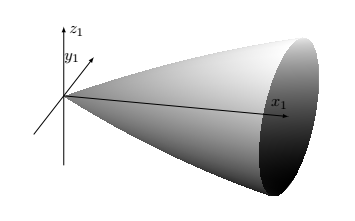
\includegraphics[width=0.9\linewidth]{ParabolicNoseConeAttempt.png}
%\end{subfigure}
\caption{Parabolic cone of constant density $\rho$, frontal thickness $l$, and cone constant $k = 3/4$, corresponding to a three-quarter parabolic nose cone.}
\end{figure}
\end{lstlisting}
\begin{figure}[H]
\begin{subfigure}[t]{0.5\textwidth}
\centering
\tdplotsetmaincoords{-20}{0} % 70 110
\tdplotsetrotatedcoords{0}{-20}{0}
\begin{tikzpicture}[scale=2, tdplot_main_coords]
\pgfmathsetmacro{\m}{0.25}
\pgfmathsetmacro{\L}{3}
\pgfmathsetmacro{\R}{\m*\L}
\pgfmathsetmacro{\K}{0.75}

% New approach is to draw curve (parabola) on xy plane and rotate plane until it matches well with base
\pgfmathsetmacro{\th}{-20}
\pgfmathsetmacro{\cost}{cos(\th)}
\pgfmathsetmacro{\sint}{sin(\th)}
\begin{scope}[tdplot_rotated_coords, canvas is plane={O(0,0,0)x(1,0,0)y(0,\cost,\sint)}]
\draw [domain=0:\L, samples=40] plot ({\x}, {((\R / (2 - \K)) * (2*\x/\L - \K * (\x/\L)^2)});
\draw [domain=0:\L, samples=40] plot ({\x}, {((-\R / (2 - \K)) * (2*\x/\L - \K * (\x/\L)^2)});
\end{scope}
% Draw face
\begin{scope}[tdplot_rotated_coords, canvas is yz plane at x=\L]
\pgfmathsetmacro{\t}{\R/6}
\draw (0, 0) circle[radius=\R];
\draw (0, 0) circle[radius=\R-\t];
\draw[->, >=stealth, thick] (-\R-0.2,0) -- (-\R,0);
\draw[->, >=stealth, thick] (-\R+\t+0.4,0) -- (-\R+\t,0) node[pos=1.1, right, xshift=1mm]{$R - r$};
\end{scope}
% Draw parameters
\draw[tdplot_rotated_coords, dashed] (0, 0, 0) -- (\L, 0, 0) node[pos=0.6, below]{$L$};
\draw[tdplot_rotated_coords, dashed] (\L, 0, 0) -- (\L, \R, 0) node[above, xshift=-0.5mm, yshift=0.5mm]{$R$};%node[midway, right, xshift=-1mm]{$R$};
%% Draw half angle
%\begin{scope}[tdplot_rotated_coords, canvas is xy plane at z=0]
%\pgfmathsetmacro{\angle}{atan(\R/\L)}
%\draw[->, >=stealth] (1.2,0) arc (0:\angle:1.225cm) node[midway, right]{$\theta_c$};
%\end{scope}

% Draw axes
\draw[->, >=latex, thick, tdplot_rotated_coords] (0, 0, 0) -- (1, 0 ,0) node[anchor=north west, xshift=-2mm]{$x_1$};
\draw[->, >=latex, thick, tdplot_rotated_coords] (0, 0, 0) -- (0, 1 ,0) node[pos=1, right]{$y_1$};
\draw[->, >=latex, thick, tdplot_rotated_coords] (0, 0, 0) -- (0, 0 ,1) node[anchor=north east, xshift=0.75mm, yshift=0.75mm]{$z_1$};
\end{tikzpicture}% NO SPACE!
\end{subfigure}
\hspace{1cm}% NO SPACE!
\begin{subfigure}[t]{0.5\textwidth}
\begin{tikzpicture}[scale=2]
% Define the same parameters as above
\pgfmathsetmacro{\m}{0.25}
\pgfmathsetmacro{\L}{3}
\pgfmathsetmacro{\R}{\m*\L}
\pgfmathsetmacro{\K}{0.75}
\pgfmathsetmacro{\t}{0.6} %\R/3

% Draw axes
\draw[->, >=latex, thick] (0,0) -- (2.1,0) node[right]{$x_1$}; %1.5
\draw[->, >=latex, thick] (0,0) -- (0,1.3) node[left]{$y_1$};

%% Draw angle
%\pgfmathsetmacro{\structAngle}{atan(\m)}
%\begin{scope}[shift={(\t,0)}]
%\draw[->, >=stealth, thick] (1, 0) arc(0:\structAngle:1) node[midway, right]{$\theta_c$};
%\end{scope}

% Outside cone
\draw [domain=0:\L, samples=40] plot ({\x}, {((\R / (2 - \K)) * (2*\x/\L - \K * (\x/\L)^2)});
\draw [domain=0:\L, samples=40] plot ({\x}, {((-\R / (2 - \K)) * (2*\x/\L - \K * (\x/\L)^2)});
% Inside cone
\draw[dashed, domain=\t:\L, samples=40] plot ({\x}, {((\R / (2 - \K)) * (2*(\x-\t)/\L - \K * ((\x-\t)/\L)^2)});
\draw[dashed, domain=\t:\L, samples=40] plot ({\x}, {((-\R / (2 - \K)) * (2*(\x-\t)/\L - \K * ((\x-\t)/\L)^2)});
% Draw t
\pgfmathsetmacro{\YofLine}{-0.33} %-0.05
\draw[dashed] (0, 0) -- (0, \YofLine);
\draw[dashed] (\t, 0) -- (\t, \YofLine);
\draw[|-|] (0,\YofLine) -- (\t,\YofLine) node[pos=0.5, below]{$l$}; %pos=0.6, below, yshift=-2.3mm

%%% Draw vertical thickness
%\pgfmathsetmacro{\XofVerticalMarker}{0.8*\L}
%\pgfmathsetmacro{\YofVerticalMarkerOnInside}{\m*(\XofVerticalMarker-\t)}
%\pgfmathsetmacro{\YofVerticalMarkerOnOutside}{\m*\XofVerticalMarker}
%\pgfmathsetmacro{\tailLength}{0.2}
%\draw[->, >=stealth] (\XofVerticalMarker, -\YofVerticalMarkerOnInside+\tailLength) -- (\XofVerticalMarker, -\YofVerticalMarkerOnInside);
%\draw[->, >=stealth] (\XofVerticalMarker, -\YofVerticalMarkerOnOutside-\tailLength) -- (\XofVerticalMarker, -\YofVerticalMarkerOnOutside) node[left, rotate=-atan(\m), xshift=-1.5mm, yshift=-2.5mm]{$\tan\theta_c \,t$};
%% Draw normal thickness
%\pgfmathsetmacro{\setXOutsideOn}{0.8*\L}
%\pgfmathsetmacro{\setYOutsideOn}{\m*\setXOutsideOn}
%\pgfmathsetmacro{\setXOutsideOff}{\setXOutsideOn-0.05}
%\pgfmathsetmacro{\setYOutsideOff}{\setYOutsideOn -1/\m * (\setXOutsideOff - \setXOutsideOn)}
%%
%\pgfmathsetmacro{\setXInsideOn}{\setXOutsideOn + \m^2*\t/(1+\m^2)}
%\pgfmathsetmacro{\setYInsideOn}{\m*(\setXInsideOn-\t)}
%\pgfmathsetmacro{\setXInsideOff}{\setXInsideOn+0.05}
%\pgfmathsetmacro{\setYInsideOff}{\setYInsideOn -1/\m * (\setXInsideOff - \setXInsideOn)}
%%
%\draw[->, >=stealth] (\setXOutsideOff, \setYOutsideOff) -- (\setXOutsideOn, \setYOutsideOn) node[left, xshift=-2mm, yshift=2mm, rotate=atan(\m)]{$|\sin\theta_c|\tan\theta_c \,t$};
%\draw[->, >=stealth] (\setXInsideOff, \setYInsideOff) -- (\setXInsideOn, \setYInsideOn);

\end{tikzpicture}
\end{subfigure}

%\begin{subfigure}[t]{0.5\textwidth}
%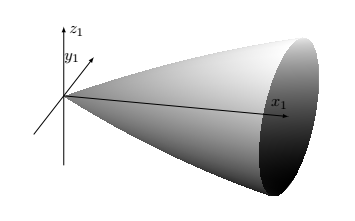
\includegraphics[width=0.9\linewidth]{ParabolicNoseConeAttempt.png}
%\end{subfigure}
\caption{Parabolic cone of constant density $\rho$, frontal thickness $l$, and cone constant $k = 3/4$, corresponding to a three-quarter parabolic nose cone.}
\end{figure}

\newpage
\subsection{Comparing Parabolic Cone to vK Ogive}
\begin{lstlisting}
\begin{figure}[H]
\centering
\begin{tikzpicture}[scale=2]
% Define the same parameters as above
\pgfmathsetmacro{\m}{0.25}
\pgfmathsetmacro{\L}{3}
\pgfmathsetmacro{\R}{\m*\L}
\pgfmathsetmacro{\K}{0.9}
\pgfmathsetmacro{\t}{0.6} %\R/3

% Draw axes
\draw[->, >=latex, thick] (0,0) -- (2.1,0) node[right]{$x_1$}; %1.5
\draw[->, >=latex, thick] (0,0) -- (0,1.3) node[left]{$y_1$};

%% Draw angle
%\pgfmathsetmacro{\structAngle}{atan(\m)}
%\begin{scope}[shift={(\t,0)}]
%\draw[->, >=stealth, thick] (1, 0) arc(0:\structAngle:1) node[midway, right]{$\theta_c$};
%\end{scope}

% Outside cone
\draw[red, domain=0:\L, samples=120] plot ({\x}, {((\R / (2 - \K)) * (2*\x/\L - \K * (\x/\L)^2)});
\draw[red, domain=0:\L, samples=120] plot ({\x}, {((-\R / (2 - \K)) * (2*\x/\L - \K * (\x/\L)^2)});
% Inside cone
\draw[red, dashed, domain=\t:\L, samples=40] plot ({\x}, {((\R / (2 - \K)) * (2*(\x-\t)/\L - \K * ((\x-\t)/\L)^2)});
\draw[red, dashed, domain=\t:\L, samples=40] plot ({\x}, {((-\R / (2 - \K)) * (2*(\x-\t)/\L - \K * ((\x-\t)/\L)^2)});
% Draw t
\pgfmathsetmacro{\YofLine}{-0.33} %-0.05
\draw[dashed] (0, 0) -- (0, \YofLine);
\draw[dashed] (\t, 0) -- (\t, \YofLine);
\draw[|-|] (0,\YofLine) -- (\t,\YofLine) node[pos=0.5, below]{$l$}; %pos=0.6, below, yshift=-2.3mm

% Draw Haack cone
\pgfmathsetmacro{\c}{0} % von Karman cone
% Outside cone
\draw [domain=0:\L, samples=120] plot ({\x}, {(\R / sqrt(pi)) * sqrt(acos(1 - 2*\x/\L)*pi/180 - sin(2*acos(1 - 2*\x/\L))/2 + \c * sin(acos(1 - 2*\x/\L))^3)});
\draw [domain=0:\L, samples=120] plot ({\x}, {(-\R / sqrt(pi)) * sqrt(acos(1 - 2*\x/\L)*pi/180 - sin(2*acos(1 - 2*\x/\L))/2 + \c * sin(acos(1 - 2*\x/\L))^3)});
% Inside cone
\draw [dashed, domain=\t:\L, samples=40] plot ({\x}, {(\R / sqrt(pi)) * sqrt(acos(1 - 2*(\x-\t)/\L)*pi/180 - sin(2*acos(1 - 2*(\x-\t)/\L))/2 + \c * sin(acos(1 - 2*(\x-\t)/\L))^3)});
\draw [dashed, domain=\t:\L, samples=40] plot ({\x}, {(-\R / sqrt(pi)) * sqrt(acos(1 - 2*(\x-\t)/\L)*pi/180 - sin(2*acos(1 - 2*(\x-\t)/\L))/2 + \c * sin(acos(1 - 2*(\x-\t)/\L))^3)});


%%% Draw vertical thickness
%\pgfmathsetmacro{\XofVerticalMarker}{0.8*\L}
%\pgfmathsetmacro{\YofVerticalMarkerOnInside}{\m*(\XofVerticalMarker-\t)}
%\pgfmathsetmacro{\YofVerticalMarkerOnOutside}{\m*\XofVerticalMarker}
%\pgfmathsetmacro{\tailLength}{0.2}
%\draw[->, >=stealth] (\XofVerticalMarker, -\YofVerticalMarkerOnInside+\tailLength) -- (\XofVerticalMarker, -\YofVerticalMarkerOnInside);
%\draw[->, >=stealth] (\XofVerticalMarker, -\YofVerticalMarkerOnOutside-\tailLength) -- (\XofVerticalMarker, -\YofVerticalMarkerOnOutside) node[left, rotate=-atan(\m), xshift=-1.5mm, yshift=-2.5mm]{$\tan\theta_c \,t$};
%% Draw normal thickness
%\pgfmathsetmacro{\setXOutsideOn}{0.8*\L}
%\pgfmathsetmacro{\setYOutsideOn}{\m*\setXOutsideOn}
%\pgfmathsetmacro{\setXOutsideOff}{\setXOutsideOn-0.05}
%\pgfmathsetmacro{\setYOutsideOff}{\setYOutsideOn -1/\m * (\setXOutsideOff - \setXOutsideOn)}
%%
%\pgfmathsetmacro{\setXInsideOn}{\setXOutsideOn + \m^2*\t/(1+\m^2)}
%\pgfmathsetmacro{\setYInsideOn}{\m*(\setXInsideOn-\t)}
%\pgfmathsetmacro{\setXInsideOff}{\setXInsideOn+0.05}
%\pgfmathsetmacro{\setYInsideOff}{\setYInsideOn -1/\m * (\setXInsideOff - \setXInsideOn)}
%%
%\draw[->, >=stealth] (\setXOutsideOff, \setYOutsideOff) -- (\setXOutsideOn, \setYOutsideOn) node[left, xshift=-2mm, yshift=2mm, rotate=atan(\m)]{$|\sin\theta_c|\tan\theta_c \,t$};
%\draw[->, >=stealth] (\setXInsideOff, \setYInsideOff) -- (\setXInsideOn, \setYInsideOn);

\end{tikzpicture}

%\begin{subfigure}[t]{0.5\textwidth}
%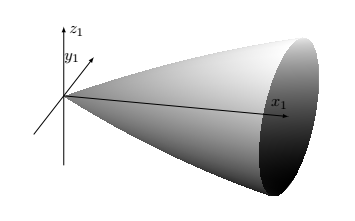
\includegraphics[width=0.9\linewidth]{ParabolicNoseConeAttempt.png}
%\end{subfigure}
\caption{Comparison of the parabolic cone of cone constant $k = 9/10$ (red, slightly inside) and the von K\'{a}rm\'{a}n ogive of the Haack series characterized by the cone constant $C = 0$ (black, slightly outside).}
\end{figure}
\end{lstlisting}
\begin{figure}[H]
\centering
\begin{tikzpicture}[scale=2]
% Define the same parameters as above
\pgfmathsetmacro{\m}{0.25}
\pgfmathsetmacro{\L}{3}
\pgfmathsetmacro{\R}{\m*\L}
\pgfmathsetmacro{\K}{0.9}
\pgfmathsetmacro{\t}{0.6} %\R/3

% Draw axes
\draw[->, >=latex, thick] (0,0) -- (2.1,0) node[right]{$x_1$}; %1.5
\draw[->, >=latex, thick] (0,0) -- (0,1.3) node[left]{$y_1$};

%% Draw angle
%\pgfmathsetmacro{\structAngle}{atan(\m)}
%\begin{scope}[shift={(\t,0)}]
%\draw[->, >=stealth, thick] (1, 0) arc(0:\structAngle:1) node[midway, right]{$\theta_c$};
%\end{scope}

% Outside cone
\draw[red, domain=0:\L, samples=120] plot ({\x}, {((\R / (2 - \K)) * (2*\x/\L - \K * (\x/\L)^2)});
\draw[red, domain=0:\L, samples=120] plot ({\x}, {((-\R / (2 - \K)) * (2*\x/\L - \K * (\x/\L)^2)});
% Inside cone
\draw[red, dashed, domain=\t:\L, samples=40] plot ({\x}, {((\R / (2 - \K)) * (2*(\x-\t)/\L - \K * ((\x-\t)/\L)^2)});
\draw[red, dashed, domain=\t:\L, samples=40] plot ({\x}, {((-\R / (2 - \K)) * (2*(\x-\t)/\L - \K * ((\x-\t)/\L)^2)});
% Draw t
\pgfmathsetmacro{\YofLine}{-0.33} %-0.05
\draw[dashed] (0, 0) -- (0, \YofLine);
\draw[dashed] (\t, 0) -- (\t, \YofLine);
\draw[|-|] (0,\YofLine) -- (\t,\YofLine) node[pos=0.5, below]{$l$}; %pos=0.6, below, yshift=-2.3mm

% Draw Haack cone
\pgfmathsetmacro{\c}{0} % von Karman cone
% Outside cone
\draw [domain=0:\L, samples=120] plot ({\x}, {(\R / sqrt(pi)) * sqrt(acos(1 - 2*\x/\L)*pi/180 - sin(2*acos(1 - 2*\x/\L))/2 + \c * sin(acos(1 - 2*\x/\L))^3)});
\draw [domain=0:\L, samples=120] plot ({\x}, {(-\R / sqrt(pi)) * sqrt(acos(1 - 2*\x/\L)*pi/180 - sin(2*acos(1 - 2*\x/\L))/2 + \c * sin(acos(1 - 2*\x/\L))^3)});
% Inside cone
\draw [dashed, domain=\t:\L, samples=40] plot ({\x}, {(\R / sqrt(pi)) * sqrt(acos(1 - 2*(\x-\t)/\L)*pi/180 - sin(2*acos(1 - 2*(\x-\t)/\L))/2 + \c * sin(acos(1 - 2*(\x-\t)/\L))^3)});
\draw [dashed, domain=\t:\L, samples=40] plot ({\x}, {(-\R / sqrt(pi)) * sqrt(acos(1 - 2*(\x-\t)/\L)*pi/180 - sin(2*acos(1 - 2*(\x-\t)/\L))/2 + \c * sin(acos(1 - 2*(\x-\t)/\L))^3)});


%%% Draw vertical thickness
%\pgfmathsetmacro{\XofVerticalMarker}{0.8*\L}
%\pgfmathsetmacro{\YofVerticalMarkerOnInside}{\m*(\XofVerticalMarker-\t)}
%\pgfmathsetmacro{\YofVerticalMarkerOnOutside}{\m*\XofVerticalMarker}
%\pgfmathsetmacro{\tailLength}{0.2}
%\draw[->, >=stealth] (\XofVerticalMarker, -\YofVerticalMarkerOnInside+\tailLength) -- (\XofVerticalMarker, -\YofVerticalMarkerOnInside);
%\draw[->, >=stealth] (\XofVerticalMarker, -\YofVerticalMarkerOnOutside-\tailLength) -- (\XofVerticalMarker, -\YofVerticalMarkerOnOutside) node[left, rotate=-atan(\m), xshift=-1.5mm, yshift=-2.5mm]{$\tan\theta_c \,t$};
%% Draw normal thickness
%\pgfmathsetmacro{\setXOutsideOn}{0.8*\L}
%\pgfmathsetmacro{\setYOutsideOn}{\m*\setXOutsideOn}
%\pgfmathsetmacro{\setXOutsideOff}{\setXOutsideOn-0.05}
%\pgfmathsetmacro{\setYOutsideOff}{\setYOutsideOn -1/\m * (\setXOutsideOff - \setXOutsideOn)}
%%
%\pgfmathsetmacro{\setXInsideOn}{\setXOutsideOn + \m^2*\t/(1+\m^2)}
%\pgfmathsetmacro{\setYInsideOn}{\m*(\setXInsideOn-\t)}
%\pgfmathsetmacro{\setXInsideOff}{\setXInsideOn+0.05}
%\pgfmathsetmacro{\setYInsideOff}{\setYInsideOn -1/\m * (\setXInsideOff - \setXInsideOn)}
%%
%\draw[->, >=stealth] (\setXOutsideOff, \setYOutsideOff) -- (\setXOutsideOn, \setYOutsideOn) node[left, xshift=-2mm, yshift=2mm, rotate=atan(\m)]{$|\sin\theta_c|\tan\theta_c \,t$};
%\draw[->, >=stealth] (\setXInsideOff, \setYInsideOff) -- (\setXInsideOn, \setYInsideOn);

\end{tikzpicture}

%\begin{subfigure}[t]{0.5\textwidth}
%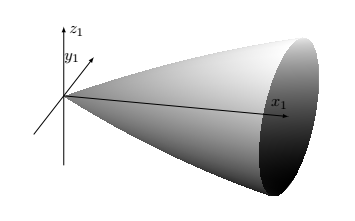
\includegraphics[width=0.9\linewidth]{ParabolicNoseConeAttempt.png}
%\end{subfigure}
\caption{Comparison of the parabolic cone of cone constant $k = 9/10$ (red, slightly inside) and the von K\'{a}rm\'{a}n ogive of the Haack series characterized by the cone constant $C = 0$ (black, slightly outside).}
\end{figure}

\newpage
\subsection{Elliptical Nose Cone}
\begin{lstlisting}
\begin{figure}[H]
\begin{subfigure}[t]{0.5\textwidth}
\centering
\tdplotsetmaincoords{-20}{0} % 70 110
\tdplotsetrotatedcoords{0}{-20}{0}
\begin{tikzpicture}[scale=2, tdplot_main_coords]
\pgfmathsetmacro{\m}{0.25}
\pgfmathsetmacro{\L}{3}
\pgfmathsetmacro{\R}{\m*\L}
\pgfmathsetmacro{\K}{0.75}

% New approach is to draw curve (parabola) on xy plane and rotate plane until it matches well with base
\pgfmathsetmacro{\th}{-20}
\pgfmathsetmacro{\cost}{cos(\th)}
\pgfmathsetmacro{\sint}{sin(\th)}
\begin{scope}[tdplot_rotated_coords, canvas is plane={O(0,0,0)x(1,0,0)y(0,\cost,\sint)}]
\draw [domain=0:\L, samples=40] plot ({\x}, {\R * sqrt(1 - ((\x-\L) / \L)^2)});
\draw [domain=0:\L, samples=40] plot ({\x}, {-\R * sqrt(1 - ((\x-\L) / \L)^2)});
\end{scope}
% Draw face
\begin{scope}[tdplot_rotated_coords, canvas is yz plane at x=\L]
\pgfmathsetmacro{\t}{\R/6}
\draw (0, 0) circle[radius=\R];
\draw (0, 0) circle[radius=\R-\t];
\draw[->, >=stealth, thick] (-\R-0.2,0) -- (-\R,0);
\draw[->, >=stealth, thick] (-\R+\t+0.4,0) -- (-\R+\t,0) node[pos=1.1, right, xshift=1mm]{$R - r$};
\end{scope}
% Draw parameters
\draw[tdplot_rotated_coords, dashed] (0, 0, 0) -- (\L, 0, 0) node[pos=0.6, below]{$L$};
\draw[tdplot_rotated_coords, dashed] (\L, 0, 0) -- (\L, \R, 0) node[above, xshift=-0.5mm, yshift=0.5mm]{$R$};%node[midway, right, xshift=-1mm]{$R$};
%% Draw half angle
%\begin{scope}[tdplot_rotated_coords, canvas is xy plane at z=0]
%\pgfmathsetmacro{\angle}{atan(\R/\L)}
%\draw[->, >=stealth] (1.2,0) arc (0:\angle:1.225cm) node[midway, right]{$\theta_c$};
%\end{scope}

% Draw axes
\draw[->, >=latex, thick, tdplot_rotated_coords] (0, 0, 0) -- (1, 0 ,0) node[anchor=north west, xshift=-2mm]{$x_1$};
\draw[->, >=latex, thick, tdplot_rotated_coords] (0, 0, 0) -- (0, 1 ,0) node[pos=1, right]{$y_1$};
\draw[->, >=latex, thick, tdplot_rotated_coords] (0, 0, 0) -- (0, 0 ,1) node[anchor=north east, xshift=0.75mm, yshift=0.75mm]{$z_1$};
\end{tikzpicture}% NO SPACE!
\end{subfigure}
\hspace{1cm}% NO SPACE!
\begin{subfigure}[t]{0.5\textwidth}
\begin{tikzpicture}[scale=2]
% Define the same parameters as above
\pgfmathsetmacro{\m}{0.25}
\pgfmathsetmacro{\L}{3}
\pgfmathsetmacro{\R}{\m*\L}
\pgfmathsetmacro{\K}{0.75}
\pgfmathsetmacro{\t}{0.6} %\R/3

% Draw axes
\draw[->, >=latex, thick] (0,0) -- (2.1,0) node[right]{$x_1$}; %1.5
\draw[->, >=latex, thick] (0,0) -- (0,1.3) node[left]{$y_1$};

%% Draw angle
%\pgfmathsetmacro{\structAngle}{atan(\m)}
%\begin{scope}[shift={(\t,0)}]
%\draw[->, >=stealth, thick] (1, 0) arc(0:\structAngle:1) node[midway, right]{$\theta_c$};
%\end{scope}

% Outside cone
\draw [domain=0:\L, samples=40] plot ({\x}, {\R * sqrt(1 - ((\x-\L) / \L)^2)});
\draw [domain=0:\L, samples=40] plot ({\x}, {-\R * sqrt(1 - ((\x-\L) / \L)^2)});
% Inside cone
\draw[dashed, domain=\t:\L, samples=40] plot ({\x}, {\R * sqrt(1 - ((\x-\t-\L) / \L)^2) * (1 - sin(180*\t/\L)^2)});
\draw[dashed, domain=\t:\L, samples=40] plot ({\x}, {-\R * sqrt(1 - ((\x-\t-\L) / \L)^2) * (1 - sin(180*\t/\L)^2)});
% Draw t
\pgfmathsetmacro{\YofLine}{-0.65} %-0.05
\draw[dashed] (0, 0) -- (0, \YofLine);
\draw[dashed] (\t, 0) -- (\t, \YofLine);
\draw[|-|] (0,\YofLine) -- (\t,\YofLine) node[pos=0.5, below]{$l$}; %pos=0.6, below, yshift=-2.3mm

%%% Draw vertical thickness
%\pgfmathsetmacro{\XofVerticalMarker}{0.8*\L}
%\pgfmathsetmacro{\YofVerticalMarkerOnInside}{\m*(\XofVerticalMarker-\t)}
%\pgfmathsetmacro{\YofVerticalMarkerOnOutside}{\m*\XofVerticalMarker}
%\pgfmathsetmacro{\tailLength}{0.2}
%\draw[->, >=stealth] (\XofVerticalMarker, -\YofVerticalMarkerOnInside+\tailLength) -- (\XofVerticalMarker, -\YofVerticalMarkerOnInside);
%\draw[->, >=stealth] (\XofVerticalMarker, -\YofVerticalMarkerOnOutside-\tailLength) -- (\XofVerticalMarker, -\YofVerticalMarkerOnOutside) node[left, rotate=-atan(\m), xshift=-1.5mm, yshift=-2.5mm]{$\tan\theta_c \,t$};
%% Draw normal thickness
%\pgfmathsetmacro{\setXOutsideOn}{0.8*\L}
%\pgfmathsetmacro{\setYOutsideOn}{\m*\setXOutsideOn}
%\pgfmathsetmacro{\setXOutsideOff}{\setXOutsideOn-0.05}
%\pgfmathsetmacro{\setYOutsideOff}{\setYOutsideOn -1/\m * (\setXOutsideOff - \setXOutsideOn)}
%%
%\pgfmathsetmacro{\setXInsideOn}{\setXOutsideOn + \m^2*\t/(1+\m^2)}
%\pgfmathsetmacro{\setYInsideOn}{\m*(\setXInsideOn-\t)}
%\pgfmathsetmacro{\setXInsideOff}{\setXInsideOn+0.05}
%\pgfmathsetmacro{\setYInsideOff}{\setYInsideOn -1/\m * (\setXInsideOff - \setXInsideOn)}
%%
%\draw[->, >=stealth] (\setXOutsideOff, \setYOutsideOff) -- (\setXOutsideOn, \setYOutsideOn) node[left, xshift=-2mm, yshift=2mm, rotate=atan(\m)]{$|\sin\theta_c|\tan\theta_c \,t$};
%\draw[->, >=stealth] (\setXInsideOff, \setYInsideOff) -- (\setXInsideOn, \setYInsideOn);

\end{tikzpicture}
\end{subfigure}

%\begin{subfigure}[t]{0.5\textwidth}
%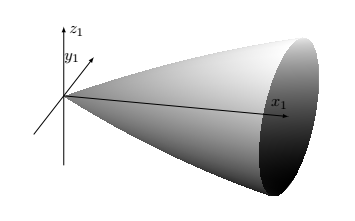
\includegraphics[width=0.9\linewidth]{ParabolicNoseConeAttempt.png}
%\end{subfigure}
\caption{Elliptical cone of constant density $\rho$ and frontal thickness $l$.}
\label{fig:StructuresEllipticalCone}
\end{figure}
\end{lstlisting}

\newpage
\subsection{Solid Cylinder}
\begin{lstlisting}
\begin{figure}[H]
\centering
\tdplotsetmaincoords{-20}{0} % 70 110
\tdplotsetrotatedcoords{0}{-20}{0}
\begin{tikzpicture}[scale=2, tdplot_main_coords]
\pgfmathsetmacro{\m}{0.25}
\pgfmathsetmacro{\L}{3}
\pgfmathsetmacro{\R}{\m*\L}

% Draw sides
\pgfmathsetmacro{\t}{-20}
\pgfmathsetmacro{\Rcost}{\R*cos(\t)}
\pgfmathsetmacro{\Rsint}{\R*sin(\t)}
\draw[tdplot_rotated_coords] (0, \Rcost, \Rsint) -- (\L, \Rcost, \Rsint);
\draw[tdplot_rotated_coords] (0, -\Rcost, -\Rsint) -- (\L, -\Rcost, -\Rsint);
% Draw faces
\begin{scope}[tdplot_rotated_coords, canvas is yz plane at x=0]
\pgfmathsetmacro{\ttmp}{145}
\pgfmathsetmacro{\Rsinttmp}{\R*sin(\ttmp)}
\pgfmathsetmacro{\Rcosttmp}{\R*cos(\ttmp)}
\draw (\Rcost, \Rsint) arc(\t:\ttmp:\R);
\draw[dashed] (\Rcosttmp, \Rsinttmp) arc(\ttmp:360:\R);
\end{scope}
\begin{scope}[tdplot_rotated_coords, canvas is yz plane at x=\L]
\draw (0, 0) circle[radius=\R];
\end{scope}
% Draw parameters
\draw[tdplot_rotated_coords, dashed] (0, 0, 0) -- (\L, 0, 0) node[pos=0.6, below]{$L$};
\draw[tdplot_rotated_coords, dashed] (\L, 0, 0) -- (\L, \R, 0) node[above, xshift=-0.5mm, yshift=0.5mm]{$R$};%node[midway, right, xshift=0mm]{$R$};

% Draw axes
\draw[->, >=latex, thick, tdplot_rotated_coords] (0, 0, 0) -- (1, 0 ,0) node[anchor=north west, xshift=-2mm]{$x_m$};
\draw[->, >=latex, thick, tdplot_rotated_coords] (0, 0, 0) -- (0, 1 ,0) node[pos=1, right]{$y_m$};
\draw[->, >=latex, thick, tdplot_rotated_coords] (0, 0, 0) -- (0, 0 ,1) node[anchor=north east, xshift=0.75mm, yshift=0.75mm]{$z_m$};
\end{tikzpicture}
\caption{Solid cylinder of constant density $\rho$.}
\end{figure}
\end{lstlisting}
\begin{figure}[H]
\centering
\tdplotsetmaincoords{-20}{0} % 70 110
\tdplotsetrotatedcoords{0}{-20}{0}
\begin{tikzpicture}[scale=2, tdplot_main_coords]
\pgfmathsetmacro{\m}{0.25}
\pgfmathsetmacro{\L}{3}
\pgfmathsetmacro{\R}{\m*\L}

% Draw sides
\pgfmathsetmacro{\t}{-20}
\pgfmathsetmacro{\Rcost}{\R*cos(\t)}
\pgfmathsetmacro{\Rsint}{\R*sin(\t)}
\draw[tdplot_rotated_coords] (0, \Rcost, \Rsint) -- (\L, \Rcost, \Rsint);
\draw[tdplot_rotated_coords] (0, -\Rcost, -\Rsint) -- (\L, -\Rcost, -\Rsint);
% Draw faces
\begin{scope}[tdplot_rotated_coords, canvas is yz plane at x=0]
\pgfmathsetmacro{\ttmp}{145}
\pgfmathsetmacro{\Rsinttmp}{\R*sin(\ttmp)}
\pgfmathsetmacro{\Rcosttmp}{\R*cos(\ttmp)}
\draw (\Rcost, \Rsint) arc(\t:\ttmp:\R);
\draw[dashed] (\Rcosttmp, \Rsinttmp) arc(\ttmp:360:\R);
\end{scope}
\begin{scope}[tdplot_rotated_coords, canvas is yz plane at x=\L]
\draw (0, 0) circle[radius=\R];
\end{scope}
% Draw parameters
\draw[tdplot_rotated_coords, dashed] (0, 0, 0) -- (\L, 0, 0) node[pos=0.6, below]{$L$};
\draw[tdplot_rotated_coords, dashed] (\L, 0, 0) -- (\L, \R, 0) node[above, xshift=-0.5mm, yshift=0.5mm]{$R$};%node[midway, right, xshift=0mm]{$R$};

% Draw axes
\draw[->, >=latex, thick, tdplot_rotated_coords] (0, 0, 0) -- (1, 0 ,0) node[anchor=north west, xshift=-2mm]{$x_m$};
\draw[->, >=latex, thick, tdplot_rotated_coords] (0, 0, 0) -- (0, 1 ,0) node[pos=1, right]{$y_m$};
\draw[->, >=latex, thick, tdplot_rotated_coords] (0, 0, 0) -- (0, 0 ,1) node[anchor=north east, xshift=0.75mm, yshift=0.75mm]{$z_m$};
\end{tikzpicture}
\caption{Solid cylinder of constant density $\rho$.}
\end{figure}

\newpage
\subsection{Hollow Cylinder}
\begin{lstlisting}
\begin{figure}[H]
\begin{subfigure}[t]{0.5\textwidth}
\centering
\tdplotsetmaincoords{-20}{0} % 70 110
\tdplotsetrotatedcoords{0}{-20}{0}
\begin{tikzpicture}[scale=2, tdplot_main_coords]
\pgfmathsetmacro{\m}{0.25}
\pgfmathsetmacro{\L}{3}
\pgfmathsetmacro{\R}{\m*\L}

% New approach is to draw curve (parabola) on xy plane and rotate plane until it matches well with base
\pgfmathsetmacro{\th}{-20}
\pgfmathsetmacro{\cost}{cos(\th)}
\pgfmathsetmacro{\sint}{sin(\th)}
\begin{scope}[tdplot_rotated_coords, canvas is plane={O(0,0,0)x(1,0,0)y(0,\cost,\sint)}]
\draw [domain=0:\L, samples=3] plot ({\x}, {\R});
\draw [domain=0:\L, samples=3] plot ({\x}, {-\R});
\end{scope}
% Draw face
\begin{scope}[tdplot_rotated_coords, canvas is yz plane at x=\L]
\pgfmathsetmacro{\t}{\R/6}
\draw (0, 0) circle[radius=\R];
\draw (0, 0) circle[radius=\R-\t];
\draw[->, >=stealth, thick] (-\R-0.2,0) -- (-\R,0);
\draw[->, >=stealth, thick] (-\R+\t+0.4,0) -- (-\R+\t,0) node[pos=1.1, right, xshift=2mm]{$R - r$};
\end{scope}
% Draw faces
%\pgfmathsetmacro{\t}{-20}
\pgfmathsetmacro{\Rcost}{\R*\cost}
\pgfmathsetmacro{\Rsint}{\R*\sint}
\begin{scope}[tdplot_rotated_coords, canvas is yz plane at x=0]
\pgfmathsetmacro{\thtmp}{145}
\pgfmathsetmacro{\Rsinttmp}{\R*sin(\thtmp)}
\pgfmathsetmacro{\Rcosttmp}{\R*cos(\thtmp)}
\draw (\Rcost, \Rsint) arc(\th:\thtmp:\R);
\draw[dashed] (\Rcosttmp, \Rsinttmp) arc(\thtmp:360:\R);
\pgfmathsetmacro{\Rminust}{\R*5/6}
\draw[dashed] (\Rminust, 0) arc(0:360:\Rminust); % Inside face
\end{scope}
% Draw parameters
\draw[tdplot_rotated_coords, dashed] (0, 0, 0) -- (\L, 0, 0) node[pos=0.6, below]{$L$};
\draw[tdplot_rotated_coords, dashed] (\L, 0, 0) -- (\L, \R, 0) node[above, xshift=-0.5mm, yshift=0.5mm]{$R$}; % node[midway, right, xshift=-1mm]{$R$};
%% Draw half angle
%\begin{scope}[tdplot_rotated_coords, canvas is xy plane at z=0]
%\pgfmathsetmacro{\angle}{atan(\R/\L)}
%\draw[->, >=stealth] (1.2,0) arc (0:\angle:1.225cm) node[midway, right]{$\theta_c$};
%\end{scope}

% Draw axes
\draw[->, >=latex, thick, tdplot_rotated_coords] (0, 0, 0) -- (1, 0 ,0) node[anchor=north west, xshift=-2mm]{$x_m$};
\draw[->, >=latex, thick, tdplot_rotated_coords] (0, 0, 0) -- (0, 1 ,0) node[pos=1, right]{$y_m$};
\draw[->, >=latex, thick, tdplot_rotated_coords] (0, 0, 0) -- (0, 0 ,1) node[anchor=north east, xshift=0.75mm, yshift=0.75mm]{$z_m$};
\end{tikzpicture}% NO SPACE!
\end{subfigure}
\hspace{1cm}% NO SPACE!
\begin{subfigure}[t]{0.5\textwidth}
\begin{tikzpicture}[scale=2]
% Define the same parameters as above
\pgfmathsetmacro{\m}{0.25}
\pgfmathsetmacro{\L}{3}
\pgfmathsetmacro{\R}{\m*\L}
\pgfmathsetmacro{\t}{\R/6} %\R/3

% Draw axes
\draw[->, >=latex, thick] (0,0) -- (2.1,0) node[right]{$x_m$}; %1.5
\draw[->, >=latex, thick] (0,0) -- (0,1.3) node[left]{$y_m$};

%% Draw angle
%\pgfmathsetmacro{\structAngle}{atan(\m)}
%\begin{scope}[shift={(\t,0)}]
%\draw[->, >=stealth, thick] (1, 0) arc(0:\structAngle:1) node[midway, right]{$\theta_c$};
%\end{scope}

% Outside cylinder
\draw [domain=0:\L, samples=3] plot ({\x}, {\R});
\draw [domain=0:\L, samples=3] plot ({\x}, {-\R});
% Inside cylinder
\draw[dashed, domain=0:\L, samples=40] plot ({\x}, {\R-\t});
\draw[dashed, domain=0:\L, samples=40] plot ({\x}, {-(\R-\t)});
%% Draw t
%\pgfmathsetmacro{\YofLine}{-0.33} %-0.05
%\draw[dashed] (0, 0) -- (0, \YofLine);
%\draw[dashed] (\t, 0) -- (\t, \YofLine);
%\draw[|-|] (0,\YofLine) -- (\t,\YofLine) node[pos=0.5, below]{$t$}; %pos=0.6, below, yshift=-2.3mm

%% Draw vertical thickness
\pgfmathsetmacro{\XofVerticalMarker}{0.8*\L}
\pgfmathsetmacro{\YofVerticalMarkerOnInside}{\R-\t}
\pgfmathsetmacro{\YofVerticalMarkerOnOutside}{\R}
\pgfmathsetmacro{\tailLength}{0.2}
\draw[->, >=stealth] (\XofVerticalMarker, \YofVerticalMarkerOnInside-\tailLength) -- (\XofVerticalMarker, \YofVerticalMarkerOnInside);
\draw[->, >=stealth] (\XofVerticalMarker, \YofVerticalMarkerOnOutside+\tailLength) -- (\XofVerticalMarker, \YofVerticalMarkerOnOutside) node[right, xshift=0.5mm, yshift=2.25mm]{$R - r$};
%% Draw normal thickness
%\pgfmathsetmacro{\setXOutsideOn}{0.8*\L}
%\pgfmathsetmacro{\setYOutsideOn}{\m*\setXOutsideOn}
%\pgfmathsetmacro{\setXOutsideOff}{\setXOutsideOn-0.05}
%\pgfmathsetmacro{\setYOutsideOff}{\setYOutsideOn -1/\m * (\setXOutsideOff - \setXOutsideOn)}
%%
%\pgfmathsetmacro{\setXInsideOn}{\setXOutsideOn + \m^2*\t/(1+\m^2)}
%\pgfmathsetmacro{\setYInsideOn}{\m*(\setXInsideOn-\t)}
%\pgfmathsetmacro{\setXInsideOff}{\setXInsideOn+0.05}
%\pgfmathsetmacro{\setYInsideOff}{\setYInsideOn -1/\m * (\setXInsideOff - \setXInsideOn)}
%%
%\draw[->, >=stealth] (\setXOutsideOff, \setYOutsideOff) -- (\setXOutsideOn, \setYOutsideOn) node[left, xshift=-2mm, yshift=2mm, rotate=atan(\m)]{$|\sin\theta_c|\tan\theta_c \,t$};
%\draw[->, >=stealth] (\setXInsideOff, \setYInsideOff) -- (\setXInsideOn, \setYInsideOn);

\end{tikzpicture}
\end{subfigure}
\caption{Hollow cylinder of constant density $\rho$ and wall thickness $R - r$.}
\end{figure}
\end{lstlisting}
\begin{figure}[H]
\begin{subfigure}[t]{0.5\textwidth}
\centering
\tdplotsetmaincoords{-20}{0} % 70 110
\tdplotsetrotatedcoords{0}{-20}{0}
\begin{tikzpicture}[scale=2, tdplot_main_coords]
\pgfmathsetmacro{\m}{0.25}
\pgfmathsetmacro{\L}{3}
\pgfmathsetmacro{\R}{\m*\L}

% New approach is to draw curve (parabola) on xy plane and rotate plane until it matches well with base
\pgfmathsetmacro{\th}{-20}
\pgfmathsetmacro{\cost}{cos(\th)}
\pgfmathsetmacro{\sint}{sin(\th)}
\begin{scope}[tdplot_rotated_coords, canvas is plane={O(0,0,0)x(1,0,0)y(0,\cost,\sint)}]
\draw [domain=0:\L, samples=3] plot ({\x}, {\R});
\draw [domain=0:\L, samples=3] plot ({\x}, {-\R});
\end{scope}
% Draw face
\begin{scope}[tdplot_rotated_coords, canvas is yz plane at x=\L]
\pgfmathsetmacro{\t}{\R/6}
\draw (0, 0) circle[radius=\R];
\draw (0, 0) circle[radius=\R-\t];
\draw[->, >=stealth, thick] (-\R-0.2,0) -- (-\R,0);
\draw[->, >=stealth, thick] (-\R+\t+0.4,0) -- (-\R+\t,0) node[pos=1.1, right, xshift=2mm]{$R - r$};
\end{scope}
% Draw faces
%\pgfmathsetmacro{\t}{-20}
\pgfmathsetmacro{\Rcost}{\R*\cost}
\pgfmathsetmacro{\Rsint}{\R*\sint}
\begin{scope}[tdplot_rotated_coords, canvas is yz plane at x=0]
\pgfmathsetmacro{\thtmp}{145}
\pgfmathsetmacro{\Rsinttmp}{\R*sin(\thtmp)}
\pgfmathsetmacro{\Rcosttmp}{\R*cos(\thtmp)}
\draw (\Rcost, \Rsint) arc(\th:\thtmp:\R);
\draw[dashed] (\Rcosttmp, \Rsinttmp) arc(\thtmp:360:\R);
\pgfmathsetmacro{\Rminust}{\R*5/6}
\draw[dashed] (\Rminust, 0) arc(0:360:\Rminust); % Inside face
\end{scope}
% Draw parameters
\draw[tdplot_rotated_coords, dashed] (0, 0, 0) -- (\L, 0, 0) node[pos=0.6, below]{$L$};
\draw[tdplot_rotated_coords, dashed] (\L, 0, 0) -- (\L, \R, 0) node[above, xshift=-0.5mm, yshift=0.5mm]{$R$}; % node[midway, right, xshift=-1mm]{$R$};
%% Draw half angle
%\begin{scope}[tdplot_rotated_coords, canvas is xy plane at z=0]
%\pgfmathsetmacro{\angle}{atan(\R/\L)}
%\draw[->, >=stealth] (1.2,0) arc (0:\angle:1.225cm) node[midway, right]{$\theta_c$};
%\end{scope}

% Draw axes
\draw[->, >=latex, thick, tdplot_rotated_coords] (0, 0, 0) -- (1, 0 ,0) node[anchor=north west, xshift=-2mm]{$x_m$};
\draw[->, >=latex, thick, tdplot_rotated_coords] (0, 0, 0) -- (0, 1 ,0) node[pos=1, right]{$y_m$};
\draw[->, >=latex, thick, tdplot_rotated_coords] (0, 0, 0) -- (0, 0 ,1) node[anchor=north east, xshift=0.75mm, yshift=0.75mm]{$z_m$};
\end{tikzpicture}% NO SPACE!
\end{subfigure}
\hspace{1cm}% NO SPACE!
\begin{subfigure}[t]{0.5\textwidth}
\begin{tikzpicture}[scale=2]
% Define the same parameters as above
\pgfmathsetmacro{\m}{0.25}
\pgfmathsetmacro{\L}{3}
\pgfmathsetmacro{\R}{\m*\L}
\pgfmathsetmacro{\t}{\R/6} %\R/3

% Draw axes
\draw[->, >=latex, thick] (0,0) -- (2.1,0) node[right]{$x_m$}; %1.5
\draw[->, >=latex, thick] (0,0) -- (0,1.3) node[left]{$y_m$};

%% Draw angle
%\pgfmathsetmacro{\structAngle}{atan(\m)}
%\begin{scope}[shift={(\t,0)}]
%\draw[->, >=stealth, thick] (1, 0) arc(0:\structAngle:1) node[midway, right]{$\theta_c$};
%\end{scope}

% Outside cylinder
\draw [domain=0:\L, samples=3] plot ({\x}, {\R});
\draw [domain=0:\L, samples=3] plot ({\x}, {-\R});
% Inside cylinder
\draw[dashed, domain=0:\L, samples=40] plot ({\x}, {\R-\t});
\draw[dashed, domain=0:\L, samples=40] plot ({\x}, {-(\R-\t)});
%% Draw t
%\pgfmathsetmacro{\YofLine}{-0.33} %-0.05
%\draw[dashed] (0, 0) -- (0, \YofLine);
%\draw[dashed] (\t, 0) -- (\t, \YofLine);
%\draw[|-|] (0,\YofLine) -- (\t,\YofLine) node[pos=0.5, below]{$t$}; %pos=0.6, below, yshift=-2.3mm

%% Draw vertical thickness
\pgfmathsetmacro{\XofVerticalMarker}{0.8*\L}
\pgfmathsetmacro{\YofVerticalMarkerOnInside}{\R-\t}
\pgfmathsetmacro{\YofVerticalMarkerOnOutside}{\R}
\pgfmathsetmacro{\tailLength}{0.2}
\draw[->, >=stealth] (\XofVerticalMarker, \YofVerticalMarkerOnInside-\tailLength) -- (\XofVerticalMarker, \YofVerticalMarkerOnInside);
\draw[->, >=stealth] (\XofVerticalMarker, \YofVerticalMarkerOnOutside+\tailLength) -- (\XofVerticalMarker, \YofVerticalMarkerOnOutside) node[right, xshift=0.5mm, yshift=2.25mm]{$R - r$};
%% Draw normal thickness
%\pgfmathsetmacro{\setXOutsideOn}{0.8*\L}
%\pgfmathsetmacro{\setYOutsideOn}{\m*\setXOutsideOn}
%\pgfmathsetmacro{\setXOutsideOff}{\setXOutsideOn-0.05}
%\pgfmathsetmacro{\setYOutsideOff}{\setYOutsideOn -1/\m * (\setXOutsideOff - \setXOutsideOn)}
%%
%\pgfmathsetmacro{\setXInsideOn}{\setXOutsideOn + \m^2*\t/(1+\m^2)}
%\pgfmathsetmacro{\setYInsideOn}{\m*(\setXInsideOn-\t)}
%\pgfmathsetmacro{\setXInsideOff}{\setXInsideOn+0.05}
%\pgfmathsetmacro{\setYInsideOff}{\setYInsideOn -1/\m * (\setXInsideOff - \setXInsideOn)}
%%
%\draw[->, >=stealth] (\setXOutsideOff, \setYOutsideOff) -- (\setXOutsideOn, \setYOutsideOn) node[left, xshift=-2mm, yshift=2mm, rotate=atan(\m)]{$|\sin\theta_c|\tan\theta_c \,t$};
%\draw[->, >=stealth] (\setXInsideOff, \setYInsideOff) -- (\setXInsideOn, \setYInsideOn);

\end{tikzpicture}
\end{subfigure}
\caption{Hollow cylinder of constant density $\rho$ and wall thickness $R - r$.}
\end{figure}

\newpage
\subsection{Hollow Frustum (Angled Hollow Cylinder)}
\begin{lstlisting}
\begin{figure}[H]
\begin{subfigure}[t]{0.5\textwidth}
\centering
\tdplotsetmaincoords{-20}{0} % 70 110
\tdplotsetrotatedcoords{0}{-20}{0}
\begin{tikzpicture}[scale=2, tdplot_main_coords]
\pgfmathsetmacro{\m}{0.25}
\pgfmathsetmacro{\L}{3}
\pgfmathsetmacro{\r}{\m*\L*0.8}
\pgfmathsetmacro{\R}{1.6*\r}

% New approach is to draw curve (parabola) on xy plane and rotate plane until it matches well with base
\pgfmathsetmacro{\th}{-20}
\pgfmathsetmacro{\cost}{cos(\th)}
\pgfmathsetmacro{\sint}{sin(\th)}
\begin{scope}[tdplot_rotated_coords, canvas is plane={O(0,0,0)x(1,0,0)y(0,\cost,\sint)}]
\draw [domain=0:\L, samples=3] plot ({\x}, {\r + ((\R - \r)/\L)*\x});
\draw [domain=0:\L, samples=3] plot ({\x}, {-(\r + ((\R - \r)/\L)*\x)});
\end{scope}
% Draw face
\pgfmathsetmacro{\t}{\R/6} %R/6
\begin{scope}[tdplot_rotated_coords, canvas is yz plane at x=\L]
\draw (0, 0) circle[radius=\R];
\draw (0, 0) circle[radius=\R-\t];
\draw[->, >=stealth, thick] (-\R-0.2,0) -- (-\R,0);
\draw[->, >=stealth, thick] (-\R+\t+0.4,0) -- (-\R+\t,0) node[pos=1.1, right, xshift=2mm]{$R - r$};
\end{scope}
% Draw faces
%\pgfmathsetmacro{\t}{-20}
\pgfmathsetmacro{\Rcost}{\R*\cost}
\pgfmathsetmacro{\Rsint}{\R*\sint}
\begin{scope}[tdplot_rotated_coords, canvas is yz plane at x=0]
\pgfmathsetmacro{\thtmp}{145}
\pgfmathsetmacro{\Rsinttmp}{\r*sin(\thtmp)}
\pgfmathsetmacro{\Rcosttmp}{\r*cos(\thtmp)}
\pgfmathsetmacro{\Rsinttmpforr}{\r*sin(-180)}
\pgfmathsetmacro{\Rcosttmpforr}{\r*cos(-180)}
\draw[dashed] (0,0) -- (\Rcosttmpforr, \Rsinttmpforr) node[below, yshift=-1mm]{$R_0$};
\draw (\r*\cost, \r*\sint) arc(\th:\thtmp:\r);
\draw[dashed] (\Rcosttmp, \Rsinttmp) arc(\thtmp:360:\r);
\pgfmathsetmacro{\Rminust}{\r-\t}
\draw[dashed] (\Rminust, 0) arc(0:360:\Rminust); % Inside face
\end{scope}
%\begin{scope}[tdplot_rotated_coords, canvas is yz plane at x=\L]
%\draw (0, 0) circle[radius=\R];
%\end{scope}
% Draw parameters
\draw[tdplot_rotated_coords, dashed] (0, 0, 0) -- (\L, 0, 0) node[pos=0.6, below]{$L$};
\draw[tdplot_rotated_coords, dashed] (\L, 0, 0) -- (\L, \R, 0) node[above, xshift=-0.5mm, yshift=0.5mm]{$R$};%node[midway, right, xshift=-1mm]{$R_L$};
%% Draw half angle
%\begin{scope}[tdplot_rotated_coords, canvas is xy plane at z=0]
%\pgfmathsetmacro{\angle}{atan(\R/\L)}
%\draw[->, >=stealth] (1.2,0) arc (0:\angle:1.225cm) node[midway, right]{$\theta_c$};
%\end{scope}

% Draw axes
\draw[->, >=latex, thick, tdplot_rotated_coords] (0, 0, 0) -- (1, 0 ,0) node[anchor=north west, xshift=-2mm]{$x_m$};
\draw[->, >=latex, thick, tdplot_rotated_coords] (0, 0, 0) -- (0, 1 ,0) node[pos=1, right]{$y_m$};
\draw[->, >=latex, thick, tdplot_rotated_coords] (0, 0, 0) -- (0, 0 ,1) node[anchor=north east, xshift=0.75mm, yshift=0.75mm]{$z_m$};
\end{tikzpicture}% NO SPACE!
\end{subfigure}
\hspace{1cm}% NO SPACE!
\begin{subfigure}[t]{0.5\textwidth}
\begin{tikzpicture}[scale=2]
% Define the same parameters as above
\pgfmathsetmacro{\m}{0.25}
\pgfmathsetmacro{\L}{3}
\pgfmathsetmacro{\r}{\m*\L*0.8}
\pgfmathsetmacro{\R}{1.6*\r}
\pgfmathsetmacro{\t}{\R/6} %\R/3

% Draw axes
\draw[->, >=latex, thick] (0,0) -- (2.1,0) node[right]{$x_m$}; %1.5
\draw[->, >=latex, thick] (0,0) -- (0,1.3) node[left]{$y_m$};

%% Draw angle
%\pgfmathsetmacro{\structAngle}{atan(\m)}
%\begin{scope}[shift={(\t,0)}]
%\draw[->, >=stealth, thick] (1, 0) arc(0:\structAngle:1) node[midway, right]{$\theta_c$};
%\end{scope}

% Outside cylinder
\draw [domain=0:\L, samples=3] plot ({\x}, {\r + ((\R - \r)/\L)*\x});
\draw [domain=0:\L, samples=3] plot ({\x}, {-(\r + ((\R - \r)/\L)*\x)});
% Inside cylinder
\draw[dashed, domain=0:\L, samples=40] plot ({\x}, {\r-\t + ((\R - \r)/\L)*(\x)});
\draw[dashed, domain=0:\L, samples=40] plot ({\x}, {-(\r-\t + ((\R - \r)/\L)*(\x))});
%% Draw t
%\pgfmathsetmacro{\YofLine}{-0.33} %-0.05
%\draw[dashed] (0, 0) -- (0, \YofLine);
%\draw[dashed] (\t, 0) -- (\t, \YofLine);
%\draw[|-|] (0,\YofLine) -- (\t,\YofLine) node[pos=0.5, below]{$t$}; %pos=0.6, below, yshift=-2.3mm

% Draw vertical thickness
\pgfmathsetmacro{\XofVerticalMarker}{0.8*\L}
\pgfmathsetmacro{\YofVerticalMarkerOnInside}{-(\r+(\R-\r)/\L*\XofVerticalMarker)}
\pgfmathsetmacro{\YofVerticalMarkerOnOutside}{-(\r-\t+(\R-\r)/\L*\XofVerticalMarker)}
\pgfmathsetmacro{\tailLength}{0.2}
\pgfmathsetmacro{\slope}{(\R - \r)/\L}
\draw[->, >=stealth] (\XofVerticalMarker, \YofVerticalMarkerOnInside-\tailLength) -- (\XofVerticalMarker, \YofVerticalMarkerOnInside) node[pos=0,left, rotate=-atan(\slope), xshift=-1.5mm, yshift=1mm]{$\tan\theta_c \,l$};
\draw[->, >=stealth] (\XofVerticalMarker, \YofVerticalMarkerOnOutside+\tailLength) -- (\XofVerticalMarker, \YofVerticalMarkerOnOutside);%node[right, xshift=1.5mm, yshift=2.5mm]{$t$};
% Draw normal thickness
\pgfmathsetmacro{\setXOutsideOn}{0.8*\L}
\pgfmathsetmacro{\setYOutsideOn}{\r + (\R - \r)/\L*\setXOutsideOn}
\pgfmathsetmacro{\setXOutsideOff}{\setXOutsideOn-0.05}
\pgfmathsetmacro{\setYOutsideOff}{\setYOutsideOn -1/\slope * (\setXOutsideOff - \setXOutsideOn)}
%
\pgfmathsetmacro{\anglef}{atan(\slope)}
\pgfmathsetmacro{\setXInsideOn}{\setXOutsideOn + \t*sin(\anglef)*cos(\anglef)}%\slope^2*\t/(1+\slope^2)}
\pgfmathsetmacro{\setYInsideOn}{-3.9*\t+(\r-\t + (\R - \r)/\L)*(\setXInsideOn)}
\pgfmathsetmacro{\setXInsideOff}{\setXInsideOn+0.05}
\pgfmathsetmacro{\setYInsideOff}{\setYInsideOn -1/\slope * (\setXInsideOff - \setXInsideOn)}
%
\draw[->, >=stealth] (\setXOutsideOff, \setYOutsideOff) -- (\setXOutsideOn, \setYOutsideOn) node[left, xshift=-2mm, yshift=2mm, rotate=atan(\slope)]{$\sin\theta_c\tan\theta_c \,l$};
\draw[->, >=stealth] (\setXInsideOff, \setYInsideOff) -- (\setXInsideOn, \setYInsideOn);

% Draw cone angle on x axis
%\pgfmathsetmacro{\xOffset}{\L * \r / (\r + \R)}
\draw[->, >=stealth, thick] (1, 0) arc(0:atan(\slope):4.6) node[midway,right]{$\theta_c$};

\end{tikzpicture}
\end{subfigure}
\caption{Hollow conical frustum of constant density $\rho$ and wall thickness $l$.}
\label{fig:StructuresHollowFrustum}
\end{figure}
\end{lstlisting}
\begin{figure}[H]
\begin{subfigure}[t]{0.5\textwidth}
\centering
\tdplotsetmaincoords{-20}{0} % 70 110
\tdplotsetrotatedcoords{0}{-20}{0}
\begin{tikzpicture}[scale=2, tdplot_main_coords]
\pgfmathsetmacro{\m}{0.25}
\pgfmathsetmacro{\L}{3}
\pgfmathsetmacro{\r}{\m*\L*0.8}
\pgfmathsetmacro{\R}{1.6*\r}

% New approach is to draw curve (parabola) on xy plane and rotate plane until it matches well with base
\pgfmathsetmacro{\th}{-20}
\pgfmathsetmacro{\cost}{cos(\th)}
\pgfmathsetmacro{\sint}{sin(\th)}
\begin{scope}[tdplot_rotated_coords, canvas is plane={O(0,0,0)x(1,0,0)y(0,\cost,\sint)}]
\draw [domain=0:\L, samples=3] plot ({\x}, {\r + ((\R - \r)/\L)*\x});
\draw [domain=0:\L, samples=3] plot ({\x}, {-(\r + ((\R - \r)/\L)*\x)});
\end{scope}
% Draw face
\pgfmathsetmacro{\t}{\R/6} %R/6
\begin{scope}[tdplot_rotated_coords, canvas is yz plane at x=\L]
\draw (0, 0) circle[radius=\R];
\draw (0, 0) circle[radius=\R-\t];
\draw[->, >=stealth, thick] (-\R-0.2,0) -- (-\R,0);
\draw[->, >=stealth, thick] (-\R+\t+0.4,0) -- (-\R+\t,0) node[pos=1.1, right, xshift=2mm]{$R - r$};
\end{scope}
% Draw faces
%\pgfmathsetmacro{\t}{-20}
\pgfmathsetmacro{\Rcost}{\R*\cost}
\pgfmathsetmacro{\Rsint}{\R*\sint}
\begin{scope}[tdplot_rotated_coords, canvas is yz plane at x=0]
\pgfmathsetmacro{\thtmp}{145}
\pgfmathsetmacro{\Rsinttmp}{\r*sin(\thtmp)}
\pgfmathsetmacro{\Rcosttmp}{\r*cos(\thtmp)}
\pgfmathsetmacro{\Rsinttmpforr}{\r*sin(-180)}
\pgfmathsetmacro{\Rcosttmpforr}{\r*cos(-180)}
\draw[dashed] (0,0) -- (\Rcosttmpforr, \Rsinttmpforr) node[below, yshift=-1mm]{$R_0$};
\draw (\r*\cost, \r*\sint) arc(\th:\thtmp:\r);
\draw[dashed] (\Rcosttmp, \Rsinttmp) arc(\thtmp:360:\r);
\pgfmathsetmacro{\Rminust}{\r-\t}
\draw[dashed] (\Rminust, 0) arc(0:360:\Rminust); % Inside face
\end{scope}
%\begin{scope}[tdplot_rotated_coords, canvas is yz plane at x=\L]
%\draw (0, 0) circle[radius=\R];
%\end{scope}
% Draw parameters
\draw[tdplot_rotated_coords, dashed] (0, 0, 0) -- (\L, 0, 0) node[pos=0.6, below]{$L$};
\draw[tdplot_rotated_coords, dashed] (\L, 0, 0) -- (\L, \R, 0) node[above, xshift=-0.5mm, yshift=0.5mm]{$R$};%node[midway, right, xshift=-1mm]{$R_L$};
%% Draw half angle
%\begin{scope}[tdplot_rotated_coords, canvas is xy plane at z=0]
%\pgfmathsetmacro{\angle}{atan(\R/\L)}
%\draw[->, >=stealth] (1.2,0) arc (0:\angle:1.225cm) node[midway, right]{$\theta_c$};
%\end{scope}

% Draw axes
\draw[->, >=latex, thick, tdplot_rotated_coords] (0, 0, 0) -- (1, 0 ,0) node[anchor=north west, xshift=-2mm]{$x_m$};
\draw[->, >=latex, thick, tdplot_rotated_coords] (0, 0, 0) -- (0, 1 ,0) node[pos=1, right]{$y_m$};
\draw[->, >=latex, thick, tdplot_rotated_coords] (0, 0, 0) -- (0, 0 ,1) node[anchor=north east, xshift=0.75mm, yshift=0.75mm]{$z_m$};
\end{tikzpicture}% NO SPACE!
\end{subfigure}
\hspace{1cm}% NO SPACE!
\begin{subfigure}[t]{0.5\textwidth}
\begin{tikzpicture}[scale=2]
% Define the same parameters as above
\pgfmathsetmacro{\m}{0.25}
\pgfmathsetmacro{\L}{3}
\pgfmathsetmacro{\r}{\m*\L*0.8}
\pgfmathsetmacro{\R}{1.6*\r}
\pgfmathsetmacro{\t}{\R/6} %\R/3

% Draw axes
\draw[->, >=latex, thick] (0,0) -- (2.1,0) node[right]{$x_m$}; %1.5
\draw[->, >=latex, thick] (0,0) -- (0,1.3) node[left]{$y_m$};

%% Draw angle
%\pgfmathsetmacro{\structAngle}{atan(\m)}
%\begin{scope}[shift={(\t,0)}]
%\draw[->, >=stealth, thick] (1, 0) arc(0:\structAngle:1) node[midway, right]{$\theta_c$};
%\end{scope}

% Outside cylinder
\draw [domain=0:\L, samples=3] plot ({\x}, {\r + ((\R - \r)/\L)*\x});
\draw [domain=0:\L, samples=3] plot ({\x}, {-(\r + ((\R - \r)/\L)*\x)});
% Inside cylinder
\draw[dashed, domain=0:\L, samples=40] plot ({\x}, {\r-\t + ((\R - \r)/\L)*(\x)});
\draw[dashed, domain=0:\L, samples=40] plot ({\x}, {-(\r-\t + ((\R - \r)/\L)*(\x))});
%% Draw t
%\pgfmathsetmacro{\YofLine}{-0.33} %-0.05
%\draw[dashed] (0, 0) -- (0, \YofLine);
%\draw[dashed] (\t, 0) -- (\t, \YofLine);
%\draw[|-|] (0,\YofLine) -- (\t,\YofLine) node[pos=0.5, below]{$t$}; %pos=0.6, below, yshift=-2.3mm

% Draw vertical thickness
\pgfmathsetmacro{\XofVerticalMarker}{0.8*\L}
\pgfmathsetmacro{\YofVerticalMarkerOnInside}{-(\r+(\R-\r)/\L*\XofVerticalMarker)}
\pgfmathsetmacro{\YofVerticalMarkerOnOutside}{-(\r-\t+(\R-\r)/\L*\XofVerticalMarker)}
\pgfmathsetmacro{\tailLength}{0.2}
\pgfmathsetmacro{\slope}{(\R - \r)/\L}
\draw[->, >=stealth] (\XofVerticalMarker, \YofVerticalMarkerOnInside-\tailLength) -- (\XofVerticalMarker, \YofVerticalMarkerOnInside) node[pos=0,left, rotate=-atan(\slope), xshift=-1.5mm, yshift=1mm]{$\tan\theta_c \,l$};
\draw[->, >=stealth] (\XofVerticalMarker, \YofVerticalMarkerOnOutside+\tailLength) -- (\XofVerticalMarker, \YofVerticalMarkerOnOutside);%node[right, xshift=1.5mm, yshift=2.5mm]{$t$};
% Draw normal thickness
\pgfmathsetmacro{\setXOutsideOn}{0.8*\L}
\pgfmathsetmacro{\setYOutsideOn}{\r + (\R - \r)/\L*\setXOutsideOn}
\pgfmathsetmacro{\setXOutsideOff}{\setXOutsideOn-0.05}
\pgfmathsetmacro{\setYOutsideOff}{\setYOutsideOn -1/\slope * (\setXOutsideOff - \setXOutsideOn)}
%
\pgfmathsetmacro{\anglef}{atan(\slope)}
\pgfmathsetmacro{\setXInsideOn}{\setXOutsideOn + \t*sin(\anglef)*cos(\anglef)}%\slope^2*\t/(1+\slope^2)}
\pgfmathsetmacro{\setYInsideOn}{-3.9*\t+(\r-\t + (\R - \r)/\L)*(\setXInsideOn)}
\pgfmathsetmacro{\setXInsideOff}{\setXInsideOn+0.05}
\pgfmathsetmacro{\setYInsideOff}{\setYInsideOn -1/\slope * (\setXInsideOff - \setXInsideOn)}
%
\draw[->, >=stealth] (\setXOutsideOff, \setYOutsideOff) -- (\setXOutsideOn, \setYOutsideOn) node[left, xshift=-2mm, yshift=2mm, rotate=atan(\slope)]{$\sin\theta_c\tan\theta_c \,l$};
\draw[->, >=stealth] (\setXInsideOff, \setYInsideOff) -- (\setXInsideOn, \setYInsideOn);

% Draw cone angle on x axis
%\pgfmathsetmacro{\xOffset}{\L * \r / (\r + \R)}
\draw[->, >=stealth, thick] (1, 0) arc(0:atan(\slope):4.6) node[midway,right]{$\theta_c$};

\end{tikzpicture}
\end{subfigure}
\caption{Hollow conical frustum of constant density $\rho$ and wall thickness $l$.}
\label{fig:StructuresHollowFrustum}
\end{figure}

\newpage
\subsection{Propellant Within the Rocket Body}
\begin{lstlisting}
\begin{figure}[H]
\centering
\begin{tikzpicture}
%% Temporary axis (comment out this bit when done)
%\draw[red] (0,0) -- (1,0);
%\draw[red] (0,0) -- (0,1);

% Draw the nozzle
\begin{axis}[width=15cm,
			height=207pt,
			at={(-6.71cm,0pt)},
			xmin=-8.5, xmax=1.5,
			ymin=-15, ymax=10,
			hide axis,
			]
%% Temporary axis (comment out this bit when done)
%\draw[blue] (0,0) -- (1,0);
%\draw[blue] (0,0) -- (0,1);
% Plot the diverging section - must keep curves as trig forms for constants to work (1 is hardcoded)
\pgfmathsetmacro{\YOfNozzleThroat}{1} % 1
\pgfmathsetmacro{\YOfNozzleExit}{2} % 3
\pgfmathsetmacro{\A}{(\YOfNozzleThroat + \YOfNozzleExit) / 2}
\pgfmathsetmacro{\B}{(\YOfNozzleThroat - \YOfNozzleExit) / 2}
\addplot[domain=0:1, samples=100, smooth, solid]{\A + \B * cos(deg(pi*x))};
\addplot[domain=0:1, samples=100, smooth, solid]{-\A - \B * cos(deg(pi*x))};
% Plot the converging part
\pgfmathsetmacro{\XOfBodyNozzleIntersection}{-0.25} % -0.25
\pgfmathsetmacro{\YOfBody}{1.5} % 1.25
\pgfmathsetmacro{\C}{(\YOfNozzleThroat + \YOfBody) / 2}
\pgfmathsetmacro{\D}{(\YOfNozzleThroat - \YOfBody) / 2}
\pgfmathsetmacro{\E}{1/\XOfBodyNozzleIntersection}
\addplot[domain=\XOfBodyNozzleIntersection:0, samples=100, smooth, solid]{\C + \D * cos(deg(\E*pi*x))};
\addplot[domain=\XOfBodyNozzleIntersection:0, samples=100, smooth, solid]{-\C - \D * cos(deg(\E*pi*x))};
% Plot the body
\pgfmathsetmacro{\XofConeBodyIntersection}{-6}
\addplot[domain=\XofConeBodyIntersection:\XOfBodyNozzleIntersection, samples=100, smooth, solid]{\YOfBody};
\addplot[domain=\XofConeBodyIntersection:\XOfBodyNozzleIntersection, samples=100, smooth, solid]{-\YOfBody};
% Plot the nose as half of an ellipse
\pgfmathsetmacro{\a}{2}
\pgfmathsetmacro{\b}{\YOfBody}
\pgfmathsetmacro{\XofNoseTip}{\XofConeBodyIntersection-\a}
\addplot[domain=\XofNoseTip:\XofConeBodyIntersection, samples=100, smooth, solid]{\b * sqrt(1 - (x - \XofConeBodyIntersection)^2 / \a^2};
\addplot[domain=\XofNoseTip:\XofConeBodyIntersection, samples=100, smooth, solid]{-\b * sqrt(1 - (x - \XofConeBodyIntersection)^2 / \a^2};

% Place an ellipse on the nozzle to show that it's open ***(only shows if axis is hidden)***
\draw (1,-\YOfNozzleExit) arc (-90:90:1.5pt and 13pt);
\draw[dashed] (1, \YOfNozzleExit) arc (90:270:1.5pt and 13pt);

%% Draw a "cutaway" to show the fuel and chamber inside
\pgfmathsetmacro{\XOfFuel}{-5}
\pgfmathsetmacro{\XOfChamberOffsetFromNozzleTubeIntersection}{0.3}
\pgfmathsetmacro{\XOfChamber}{\XOfBodyNozzleIntersection-\XOfChamberOffsetFromNozzleTubeIntersection}
\pgfmathsetmacro{\YOffsetFromWall}{0.3}
\draw[fill=red!80!black!30] (\XOfFuel,\YOfBody) arc (90:-90:0.6pt and 8.7pt) -- (\XOfChamber, -\YOfBody+\YOffsetFromWall) arc (-90:90:1.2pt and 8.7pt) -- (\XOfFuel,\YOfBody) node[midway, above]{fuel};
\draw[fill=red!80!black!60] (\XOfChamber, \YOfBody) arc (90:-90:1.2pt and 8.7pt) -- (\XOfBodyNozzleIntersection, -\YOfBody+\YOffsetFromWall) arc (-90:90:1.4pt and 8.7pt) -- (\XOfChamber, \YOfBody) node[midway, above]{chamber};

% Draw an axis at the bottom to display various points along the rocket (n, t, e)
\pgfmathsetmacro{\YOfXLine}{-\YOfBody-1.6}
\pgfmathsetmacro{\tickHeight}{1}
\pgfmathsetmacro{\XOfChamberTick}{\XOfChamber + 0.16}
\draw (\XofNoseTip, \YOfXLine) -- (1, \YOfXLine);
\draw (\XofNoseTip, \YOfXLine-\tickHeight/2) -- (\XofConeBodyIntersection-\a, \YOfXLine+\tickHeight/2) node[below, yshift=-2.65mm]{$n$}; % yshift=-2.6mm
\draw (0, \YOfXLine-\tickHeight/2) -- (0, \YOfXLine+\tickHeight/2) node[below, yshift=-2mm]{$t$}; % yshift=-2mm
\draw (\XOfChamberTick, \YOfXLine-\tickHeight/2) -- (\XOfChamberTick, \YOfXLine+\tickHeight/2) node[below, yshift=-2.65mm]{$c$}; % yshift=-2.75mm
\draw (1, \YOfXLine-\tickHeight/2) -- (1, \YOfXLine+\tickHeight/2) node[below, yshift=-2.65mm]{$e$}; % yshift=-2.75mm

% Draw pressures
\draw[->, >=latex] (\XofNoseTip-1.5, 0) -- (\XofNoseTip, 0);% node[above, xshift=-4mm]{$p_n$};
\draw[->, >=latex] (2.5, \YOfNozzleExit) -- (1, \YOfNozzleExit);
\draw[->, >=latex] (2.5, \YOfNozzleExit/2) -- (1, \YOfNozzleExit/2);
\draw[->, >=latex] (2.5, 0) -- (1, 0);% node[above, xshift=4mm]{$p_e$};
\draw[->, >=latex] (2.5, -\YOfNozzleExit) -- (1, -\YOfNozzleExit);
\draw[->, >=latex] (2.5, -\YOfNozzleExit/2) -- (1, -\YOfNozzleExit/2);

% Draw mass flow rate
\draw[->, >=latex, dashed] (0,0) -- (0.4, 0) node[right]{$\dot{m}$};

%% Draw shock
%% Commented this out since it really concerns aerodynamics
%\addplot[domain=\XofNoseTip-0.05:\XofNoseTip+1, samples=250, smooth, solid]{sqrt(1 - (x - (\XofConeBodyIntersection-0.05))^2 / \a^2) * (\b+1.6)};

% Draw center of mass for v and F
\pgfmathsetmacro{\xcom}{-2.6}
\pgfmathsetmacro{\ycom}{0}
\pgfmathsetmacro{\rcom}{\YOfBody/4}
\draw (\xcom, \ycom) node[circle, fill, inner sep=1]{};
\draw[->, >=latex] (\xcom, \ycom) -- (\xcom-0.4, \ycom) node[left]{$\hat{v}$};
%\draw[->, >=latex] (\xcom+0.6, \ycom) -- (\xcom, \ycom) node[pos=0,right]{$\vec{F}_T$};
\end{axis}

% Try to draw center of mass
\begin{scope}[shift={(1.2,2.415)}] % (1.2, 2.4225)
\pgfmathsetmacro{\Bx}{0}
\pgfmathsetmacro{\By}{1}
\pgfmathsetmacro{\Br}{0.11}
\draw[fill=black] (\Bx,\By) ++(0:\Br)   arc (0:90:\Br)    -- (\Bx,\By) -- cycle;
\draw[fill=white] (\Bx,\By) ++(90:\Br)  arc (90:180:\Br)  -- (\Bx,\By) -- cycle;
\draw[fill=black] (\Bx,\By) ++(180:\Br) arc (180:270:\Br) -- (\Bx,\By) -- cycle;
\draw[fill=white] (\Bx,\By) ++(270:\Br) arc (270:360:\Br) -- (\Bx,\By) -- cycle;
\end{scope}

% Draw pressure on nose and exit
\node at (7,3.4){$p_e$};
\node at (-7,3.4){$p_n$};
    % more arrows here
\end{tikzpicture}
\caption{Overviewing diagram of the systems and quantities relevant to the basics of rocket propulsion. Particularly, this diagram contains no aerodynamic considerations (shockwaves) in the visualization of $p_n$ nor in the exhaust field. The fuel is represented by a block-cutaway to reserve space for either solid propellant or liquid fuel and oxidizer. The chamber, leading into the nozzle, is characterized by a constant total pressure, total temperature, and total density. The exhaust velocity is not shown since its reference frame (the rocket) is different from the reference frame monitoring the velocity and thrust force. The exit area $A_e$ is simply the cross-sectional area of the nozzle at the exit.}
\label{fig:PropFuelRocket}
\end{figure}
\end{lstlisting}
\begin{figure}[H]
\centering
\begin{tikzpicture}
%% Temporary axis (comment out this bit when done)
%\draw[red] (0,0) -- (1,0);
%\draw[red] (0,0) -- (0,1);

% Draw the nozzle
\begin{axis}[width=15cm,
			height=207pt,
			at={(-6.71cm,0pt)},
			xmin=-8.5, xmax=1.5,
			ymin=-15, ymax=10,
			hide axis,
			]
%% Temporary axis (comment out this bit when done)
%\draw[blue] (0,0) -- (1,0);
%\draw[blue] (0,0) -- (0,1);
% Plot the diverging section - must keep curves as trig forms for constants to work (1 is hardcoded)
\pgfmathsetmacro{\YOfNozzleThroat}{1} % 1
\pgfmathsetmacro{\YOfNozzleExit}{2} % 3
\pgfmathsetmacro{\A}{(\YOfNozzleThroat + \YOfNozzleExit) / 2}
\pgfmathsetmacro{\B}{(\YOfNozzleThroat - \YOfNozzleExit) / 2}
\addplot[domain=0:1, samples=100, smooth, solid]{\A + \B * cos(deg(pi*x))};
\addplot[domain=0:1, samples=100, smooth, solid]{-\A - \B * cos(deg(pi*x))};
% Plot the converging part
\pgfmathsetmacro{\XOfBodyNozzleIntersection}{-0.25} % -0.25
\pgfmathsetmacro{\YOfBody}{1.5} % 1.25
\pgfmathsetmacro{\C}{(\YOfNozzleThroat + \YOfBody) / 2}
\pgfmathsetmacro{\D}{(\YOfNozzleThroat - \YOfBody) / 2}
\pgfmathsetmacro{\E}{1/\XOfBodyNozzleIntersection}
\addplot[domain=\XOfBodyNozzleIntersection:0, samples=100, smooth, solid]{\C + \D * cos(deg(\E*pi*x))};
\addplot[domain=\XOfBodyNozzleIntersection:0, samples=100, smooth, solid]{-\C - \D * cos(deg(\E*pi*x))};
% Plot the body
\pgfmathsetmacro{\XofConeBodyIntersection}{-6}
\addplot[domain=\XofConeBodyIntersection:\XOfBodyNozzleIntersection, samples=100, smooth, solid]{\YOfBody};
\addplot[domain=\XofConeBodyIntersection:\XOfBodyNozzleIntersection, samples=100, smooth, solid]{-\YOfBody};
% Plot the nose as half of an ellipse
\pgfmathsetmacro{\a}{2}
\pgfmathsetmacro{\b}{\YOfBody}
\pgfmathsetmacro{\XofNoseTip}{\XofConeBodyIntersection-\a}
\addplot[domain=\XofNoseTip:\XofConeBodyIntersection, samples=100, smooth, solid]{\b * sqrt(1 - (x - \XofConeBodyIntersection)^2 / \a^2};
\addplot[domain=\XofNoseTip:\XofConeBodyIntersection, samples=100, smooth, solid]{-\b * sqrt(1 - (x - \XofConeBodyIntersection)^2 / \a^2};

% Place an ellipse on the nozzle to show that it's open ***(only shows if axis is hidden)***
\draw (1,-\YOfNozzleExit) arc (-90:90:1.5pt and 13pt);
\draw[dashed] (1, \YOfNozzleExit) arc (90:270:1.5pt and 13pt);

%% Draw a "cutaway" to show the fuel and chamber inside
\pgfmathsetmacro{\XOfFuel}{-5}
\pgfmathsetmacro{\XOfChamberOffsetFromNozzleTubeIntersection}{0.3}
\pgfmathsetmacro{\XOfChamber}{\XOfBodyNozzleIntersection-\XOfChamberOffsetFromNozzleTubeIntersection}
\pgfmathsetmacro{\YOffsetFromWall}{0.3}
\draw[fill=red!80!black!30] (\XOfFuel,\YOfBody) arc (90:-90:0.6pt and 8.7pt) -- (\XOfChamber, -\YOfBody+\YOffsetFromWall) arc (-90:90:1.2pt and 8.7pt) -- (\XOfFuel,\YOfBody) node[midway, above]{fuel};
\draw[fill=red!80!black!60] (\XOfChamber, \YOfBody) arc (90:-90:1.2pt and 8.7pt) -- (\XOfBodyNozzleIntersection, -\YOfBody+\YOffsetFromWall) arc (-90:90:1.4pt and 8.7pt) -- (\XOfChamber, \YOfBody) node[midway, above]{chamber};

% Draw an axis at the bottom to display various points along the rocket (n, t, e)
\pgfmathsetmacro{\YOfXLine}{-\YOfBody-1.6}
\pgfmathsetmacro{\tickHeight}{1}
\pgfmathsetmacro{\XOfChamberTick}{\XOfChamber + 0.16}
\draw (\XofNoseTip, \YOfXLine) -- (1, \YOfXLine);
\draw (\XofNoseTip, \YOfXLine-\tickHeight/2) -- (\XofConeBodyIntersection-\a, \YOfXLine+\tickHeight/2) node[below, yshift=-2.65mm]{$n$}; % yshift=-2.6mm
\draw (0, \YOfXLine-\tickHeight/2) -- (0, \YOfXLine+\tickHeight/2) node[below, yshift=-2mm]{$t$}; % yshift=-2mm
\draw (\XOfChamberTick, \YOfXLine-\tickHeight/2) -- (\XOfChamberTick, \YOfXLine+\tickHeight/2) node[below, yshift=-2.65mm]{$c$}; % yshift=-2.75mm
\draw (1, \YOfXLine-\tickHeight/2) -- (1, \YOfXLine+\tickHeight/2) node[below, yshift=-2.65mm]{$e$}; % yshift=-2.75mm

% Draw pressures
\draw[->, >=latex] (\XofNoseTip-1.5, 0) -- (\XofNoseTip, 0);% node[above, xshift=-4mm]{$p_n$};
\draw[->, >=latex] (2.5, \YOfNozzleExit) -- (1, \YOfNozzleExit);
\draw[->, >=latex] (2.5, \YOfNozzleExit/2) -- (1, \YOfNozzleExit/2);
\draw[->, >=latex] (2.5, 0) -- (1, 0);% node[above, xshift=4mm]{$p_e$};
\draw[->, >=latex] (2.5, -\YOfNozzleExit) -- (1, -\YOfNozzleExit);
\draw[->, >=latex] (2.5, -\YOfNozzleExit/2) -- (1, -\YOfNozzleExit/2);

% Draw mass flow rate
\draw[->, >=latex, dashed] (0,0) -- (0.4, 0) node[right]{$\dot{m}$};

%% Draw shock
%% Commented this out since it really concerns aerodynamics
%\addplot[domain=\XofNoseTip-0.05:\XofNoseTip+1, samples=250, smooth, solid]{sqrt(1 - (x - (\XofConeBodyIntersection-0.05))^2 / \a^2) * (\b+1.6)};

% Draw center of mass for v and F
\pgfmathsetmacro{\xcom}{-2.6}
\pgfmathsetmacro{\ycom}{0}
\pgfmathsetmacro{\rcom}{\YOfBody/4}
\draw (\xcom, \ycom) node[circle, fill, inner sep=1]{};
\draw[->, >=latex] (\xcom, \ycom) -- (\xcom-0.4, \ycom) node[left]{$\hat{v}$};
%\draw[->, >=latex] (\xcom+0.6, \ycom) -- (\xcom, \ycom) node[pos=0,right]{$\vec{F}_T$};
\end{axis}

% Try to draw center of mass
\begin{scope}[shift={(1.2,2.415)}] % (1.2, 2.4225)
\pgfmathsetmacro{\Bx}{0}
\pgfmathsetmacro{\By}{1}
\pgfmathsetmacro{\Br}{0.11}
\draw[fill=black] (\Bx,\By) ++(0:\Br)   arc (0:90:\Br)    -- (\Bx,\By) -- cycle;
\draw[fill=white] (\Bx,\By) ++(90:\Br)  arc (90:180:\Br)  -- (\Bx,\By) -- cycle;
\draw[fill=black] (\Bx,\By) ++(180:\Br) arc (180:270:\Br) -- (\Bx,\By) -- cycle;
\draw[fill=white] (\Bx,\By) ++(270:\Br) arc (270:360:\Br) -- (\Bx,\By) -- cycle;
\end{scope}

% Draw pressure on nose and exit
\node at (7,3.4){$p_e$};
\node at (-7,3.4){$p_n$};
    % more arrows here
\end{tikzpicture}
\caption{Overviewing diagram of the systems and quantities relevant to the basics of rocket propulsion. Particularly, this diagram contains no aerodynamic considerations (shockwaves) in the visualization of $p_n$ nor in the exhaust field. The fuel is represented by a block-cutaway to reserve space for either solid propellant or liquid fuel and oxidizer. The chamber, leading into the nozzle, is characterized by a constant total pressure, total temperature, and total density. The exhaust velocity is not shown since its reference frame (the rocket) is different from the reference frame monitoring the velocity and thrust force. The exit area $A_e$ is simply the cross-sectional area of the nozzle at the exit.}
\label{fig:PropFuelRocket}
\end{figure}

\newpage
\subsection{Nozzle Flow Coordinates and Symbol Definitions}
\begin{lstlisting}
\begin{figure}[H]
\centering
\begin{tikzpicture}
%% Temporary axis (comment out this bit when done)
%\draw[red] (0,0) -- (1,0);
%\draw[red] (0,0) -- (0,1);

% Draw the nozzle
\begin{axis}[width=15cm,
			height=207pt,
			at={(-6.71cm,0pt)},
			xmin=-1.05, xmax=1.5,
			ymin=-5, ymax=5,
			hide axis,
			]
%% Temporary axis (comment out this bit when done)
%\draw[blue] (0,0) -- (1,0);
%\draw[blue] (0,0) -- (0,1);
% Plot the diverging section - must keep curves as trig forms for constants to work (1 is hardcoded)
\pgfmathsetmacro{\YOfNozzleThroat}{1} % 1
\pgfmathsetmacro{\YOfNozzleExit}{3} % 3 | 2 | 2.5
\pgfmathsetmacro{\A}{(\YOfNozzleThroat + \YOfNozzleExit) / 2}
\pgfmathsetmacro{\B}{(\YOfNozzleThroat - \YOfNozzleExit) / 2}
\addplot[domain=0:1, samples=100, smooth, solid]{\A + \B * cos(deg(pi*x))};
\addplot[domain=0:1, samples=100, smooth, solid]{-\A - \B * cos(deg(pi*x))};
% Plot the converging part
\pgfmathsetmacro{\XOfBodyNozzleIntersection}{-0.25} % -0.25
\pgfmathsetmacro{\YOfBody}{1.5} % 1.25
\pgfmathsetmacro{\C}{(\YOfNozzleThroat + \YOfBody) / 2}
\pgfmathsetmacro{\D}{(\YOfNozzleThroat - \YOfBody) / 2}
\pgfmathsetmacro{\E}{1/\XOfBodyNozzleIntersection}
\addplot[domain=\XOfBodyNozzleIntersection:0, samples=100, smooth, solid]{\C + \D * cos(deg(\E*pi*x))};
\addplot[domain=\XOfBodyNozzleIntersection:0, samples=100, smooth, solid]{-\C - \D * cos(deg(\E*pi*x))};
% Plot the chamber
\pgfmathsetmacro{\XOfFuel}{-5}
\pgfmathsetmacro{\XOfChamberOffsetFromNozzleTubeIntersection}{0}
\pgfmathsetmacro{\XOfChamber}{\XOfBodyNozzleIntersection-\XOfChamberOffsetFromNozzleTubeIntersection}
\pgfmathsetmacro{\YOffsetFromWall}{0.3}
\pgfmathsetmacro{\XofConeBodyIntersection}{-0.4}
\addplot[domain=\XofConeBodyIntersection:\XOfBodyNozzleIntersection, samples=100, smooth, solid]{\YOfBody};
\addplot[domain=\XofConeBodyIntersection:\XOfBodyNozzleIntersection, samples=100, smooth, solid]{-\YOfBody};
% Plot the nose as half of an ellipse
\pgfmathsetmacro{\a}{2}
\pgfmathsetmacro{\b}{\YOfBody}
%\pgfmathsetmacro{\XofNoseTip}{\XofConeBodyIntersection-\a}
%\addplot[domain=\XofNoseTip:\XofConeBodyIntersection, samples=100, smooth, solid]{\b * sqrt(1 - (x - \XofConeBodyIntersection)^2 / \a^2};
%\addplot[domain=\XofNoseTip:\XofConeBodyIntersection, samples=100, smooth, solid]{-\b * sqrt(1 - (x - \XofConeBodyIntersection)^2 / \a^2};

% Place an ellipse on the nozzle to show that it's open ***(only shows if axis is hidden)***
\draw (1,-\YOfNozzleExit) arc (-90:90:1.5pt and 48.5pt);
\draw[dashed] (1, \YOfNozzleExit) arc (90:270:1.5pt and 48.5pt);

% Place an ellipse on the throat to show that it's open
\draw[dashed] (0,-\YOfNozzleThroat) arc (-90:90:1.5pt and 16pt);
\draw (0, \YOfNozzleThroat) arc (90:270:1.5pt and 16pt);


%% Draw a "cutaway" to show the fuel and chamber inside
%\draw[fill=red!80!black!30] (\XOfFuel,\YOfBody) arc (90:-90:0.6pt and 8.7pt) -- (\XOfChamber, -\YOfBody+\YOffsetFromWall) arc (-90:90:1.2pt and 8.7pt) -- (\XOfFuel,\YOfBody) node[midway, above]{fuel};
%\draw[fill=red!80!black!60] (\XOfChamber, \YOfBody) arc (90:-90:1.2pt and 8.7pt) -- (\XOfBodyNozzleIntersection, -\YOfBody+\YOffsetFromWall) arc (-90:90:1.4pt and 8.7pt) -- (\XOfChamber, \YOfBody) node[midway, above]{chamber};

% Draw an axis at the bottom to display various points along the rocket (n, t, e)
\pgfmathsetmacro{\YOfXLine}{-\YOfBody-1.6-1}
\pgfmathsetmacro{\tickHeight}{0.6}
\draw (\XOfChamber, \YOfXLine) -- (1, \YOfXLine);
\draw (\XOfChamber, \YOfXLine-\tickHeight/2) -- (\XOfChamber, \YOfXLine+\tickHeight/2) node[below, yshift=-3.7mm]{$c$};
\draw (0, \YOfXLine-\tickHeight/2) -- (0, \YOfXLine+\tickHeight/2) node[below, yshift=-3.3mm]{$t$} node[above]{$x = 0$};
\draw (1, \YOfXLine-\tickHeight/2) -- (1, \YOfXLine+\tickHeight/2) node[below, yshift=-3.7mm]{$e$} node[above]{$x = 1$};

% Draw pressure p_e
%\draw[->, >=latex] (2.5, 0) -- (1, 0) node[above, xshift=4mm]{$p_e$};

% Draw mass flow rate
%\draw[->, >=latex, dashed] (0,0) -- (0.4, 0) node[right]{$\dot{m}$};

%% Draw shock
%% Commented this out since it really concerns aerodynamics
%\addplot[domain=\XofNoseTip-0.05:\XofNoseTip+1, samples=250, smooth, solid]{sqrt(1 - (x - (\XofConeBodyIntersection-0.05))^2 / \a^2) * (\b+1.6)};
\end{axis}
\end{tikzpicture}
\caption{Nondimensionalization of the quasi-unidimensional flow coordinate frame, where the throat is at $x = 0$ and the exit is at $x = 1$. The chamber is not designated a coordinate in terms of $x$, but the subscript $c$ is important nonetheless in the determination of the flow.}
\end{figure}
\end{lstlisting}
\begin{figure}[H]
\centering
\begin{tikzpicture}
%% Temporary axis (comment out this bit when done)
%\draw[red] (0,0) -- (1,0);
%\draw[red] (0,0) -- (0,1);

% Draw the nozzle
\begin{axis}[width=15cm,
			height=207pt,
			at={(-6.71cm,0pt)},
			xmin=-1.05, xmax=1.5,
			ymin=-5, ymax=5,
			hide axis,
			]
%% Temporary axis (comment out this bit when done)
%\draw[blue] (0,0) -- (1,0);
%\draw[blue] (0,0) -- (0,1);
% Plot the diverging section - must keep curves as trig forms for constants to work (1 is hardcoded)
\pgfmathsetmacro{\YOfNozzleThroat}{1} % 1
\pgfmathsetmacro{\YOfNozzleExit}{3} % 3 | 2 | 2.5
\pgfmathsetmacro{\A}{(\YOfNozzleThroat + \YOfNozzleExit) / 2}
\pgfmathsetmacro{\B}{(\YOfNozzleThroat - \YOfNozzleExit) / 2}
\addplot[domain=0:1, samples=100, smooth, solid]{\A + \B * cos(deg(pi*x))};
\addplot[domain=0:1, samples=100, smooth, solid]{-\A - \B * cos(deg(pi*x))};
% Plot the converging part
\pgfmathsetmacro{\XOfBodyNozzleIntersection}{-0.25} % -0.25
\pgfmathsetmacro{\YOfBody}{1.5} % 1.25
\pgfmathsetmacro{\C}{(\YOfNozzleThroat + \YOfBody) / 2}
\pgfmathsetmacro{\D}{(\YOfNozzleThroat - \YOfBody) / 2}
\pgfmathsetmacro{\E}{1/\XOfBodyNozzleIntersection}
\addplot[domain=\XOfBodyNozzleIntersection:0, samples=100, smooth, solid]{\C + \D * cos(deg(\E*pi*x))};
\addplot[domain=\XOfBodyNozzleIntersection:0, samples=100, smooth, solid]{-\C - \D * cos(deg(\E*pi*x))};
% Plot the chamber
\pgfmathsetmacro{\XOfFuel}{-5}
\pgfmathsetmacro{\XOfChamberOffsetFromNozzleTubeIntersection}{0}
\pgfmathsetmacro{\XOfChamber}{\XOfBodyNozzleIntersection-\XOfChamberOffsetFromNozzleTubeIntersection}
\pgfmathsetmacro{\YOffsetFromWall}{0.3}
\pgfmathsetmacro{\XofConeBodyIntersection}{-0.4}
\addplot[domain=\XofConeBodyIntersection:\XOfBodyNozzleIntersection, samples=100, smooth, solid]{\YOfBody};
\addplot[domain=\XofConeBodyIntersection:\XOfBodyNozzleIntersection, samples=100, smooth, solid]{-\YOfBody};
% Plot the nose as half of an ellipse
\pgfmathsetmacro{\a}{2}
\pgfmathsetmacro{\b}{\YOfBody}
%\pgfmathsetmacro{\XofNoseTip}{\XofConeBodyIntersection-\a}
%\addplot[domain=\XofNoseTip:\XofConeBodyIntersection, samples=100, smooth, solid]{\b * sqrt(1 - (x - \XofConeBodyIntersection)^2 / \a^2};
%\addplot[domain=\XofNoseTip:\XofConeBodyIntersection, samples=100, smooth, solid]{-\b * sqrt(1 - (x - \XofConeBodyIntersection)^2 / \a^2};

% Place an ellipse on the nozzle to show that it's open ***(only shows if axis is hidden)***
\draw (1,-\YOfNozzleExit) arc (-90:90:1.5pt and 48.5pt);
\draw[dashed] (1, \YOfNozzleExit) arc (90:270:1.5pt and 48.5pt);

% Place an ellipse on the throat to show that it's open
\draw[dashed] (0,-\YOfNozzleThroat) arc (-90:90:1.5pt and 16pt);
\draw (0, \YOfNozzleThroat) arc (90:270:1.5pt and 16pt);


%% Draw a "cutaway" to show the fuel and chamber inside
%\draw[fill=red!80!black!30] (\XOfFuel,\YOfBody) arc (90:-90:0.6pt and 8.7pt) -- (\XOfChamber, -\YOfBody+\YOffsetFromWall) arc (-90:90:1.2pt and 8.7pt) -- (\XOfFuel,\YOfBody) node[midway, above]{fuel};
%\draw[fill=red!80!black!60] (\XOfChamber, \YOfBody) arc (90:-90:1.2pt and 8.7pt) -- (\XOfBodyNozzleIntersection, -\YOfBody+\YOffsetFromWall) arc (-90:90:1.4pt and 8.7pt) -- (\XOfChamber, \YOfBody) node[midway, above]{chamber};

% Draw an axis at the bottom to display various points along the rocket (n, t, e)
\pgfmathsetmacro{\YOfXLine}{-\YOfBody-1.6-1}
\pgfmathsetmacro{\tickHeight}{0.6}
\draw (\XOfChamber, \YOfXLine) -- (1, \YOfXLine);
\draw (\XOfChamber, \YOfXLine-\tickHeight/2) -- (\XOfChamber, \YOfXLine+\tickHeight/2) node[below, yshift=-3.7mm]{$c$};
\draw (0, \YOfXLine-\tickHeight/2) -- (0, \YOfXLine+\tickHeight/2) node[below, yshift=-3.3mm]{$t$} node[above]{$x = 0$};
\draw (1, \YOfXLine-\tickHeight/2) -- (1, \YOfXLine+\tickHeight/2) node[below, yshift=-3.7mm]{$e$} node[above]{$x = 1$};

% Draw pressure p_e
%\draw[->, >=latex] (2.5, 0) -- (1, 0) node[above, xshift=4mm]{$p_e$};

% Draw mass flow rate
%\draw[->, >=latex, dashed] (0,0) -- (0.4, 0) node[right]{$\dot{m}$};

%% Draw shock
%% Commented this out since it really concerns aerodynamics
%\addplot[domain=\XofNoseTip-0.05:\XofNoseTip+1, samples=250, smooth, solid]{sqrt(1 - (x - (\XofConeBodyIntersection-0.05))^2 / \a^2) * (\b+1.6)};
\end{axis}
\end{tikzpicture}
\caption{Nondimensionalization of the quasi-unidimensional flow coordinate frame, where the throat is at $x = 0$ and the exit is at $x = 1$. The chamber is not designated a coordinate in terms of $x$, but the subscript $c$ is important nonetheless in the determination of the flow.}
\end{figure}

\newpage
\subsection{Normal Shock in Nozzle}
\begin{lstlisting}
\begin{figure}[H]
\centering
\begin{tikzpicture}
%% Temporary axis (comment out this bit when done)
%\draw[red] (0,0) -- (1,0);
%\draw[red] (0,0) -- (0,1);

% Draw the nozzle
\begin{axis}[width=15cm,
			height=207pt,
			at={(-6.71cm,0pt)},
			xmin=-1.05, xmax=1.5,
			ymin=-5, ymax=5,
			hide axis,
			]
%% Temporary axis (comment out this bit when done)
%\draw[blue] (0,0) -- (1,0);
%\draw[blue] (0,0) -- (0,1);
% Plot the diverging section - must keep curves as trig forms for constants to work (1 is hardcoded)
\pgfmathsetmacro{\YOfNozzleThroat}{1} % 1
\pgfmathsetmacro{\YOfNozzleExit}{3} % 3 | 2 | 2.5
\pgfmathsetmacro{\A}{(\YOfNozzleThroat + \YOfNozzleExit) / 2}
\pgfmathsetmacro{\B}{(\YOfNozzleThroat - \YOfNozzleExit) / 2}
\addplot[domain=0:1, samples=100, smooth, solid]{\A + \B * cos(deg(pi*x))};
\addplot[domain=0:1, samples=100, smooth, solid]{-\A - \B * cos(deg(pi*x))};
% Plot the converging part
\pgfmathsetmacro{\XOfBodyNozzleIntersection}{-0.25} % -0.25
\pgfmathsetmacro{\YOfBody}{1.5} % 1.25
\pgfmathsetmacro{\C}{(\YOfNozzleThroat + \YOfBody) / 2}
\pgfmathsetmacro{\D}{(\YOfNozzleThroat - \YOfBody) / 2}
\pgfmathsetmacro{\E}{1/\XOfBodyNozzleIntersection}
\addplot[domain=\XOfBodyNozzleIntersection:0, samples=100, smooth, solid]{\C + \D * cos(deg(\E*pi*x))};
\addplot[domain=\XOfBodyNozzleIntersection:0, samples=100, smooth, solid]{-\C - \D * cos(deg(\E*pi*x))};
% Plot the chamber
\pgfmathsetmacro{\XOfFuel}{-5}
\pgfmathsetmacro{\XOfChamberOffsetFromNozzleTubeIntersection}{0}
\pgfmathsetmacro{\XOfChamber}{\XOfBodyNozzleIntersection-\XOfChamberOffsetFromNozzleTubeIntersection}
\pgfmathsetmacro{\YOffsetFromWall}{0.3}
\pgfmathsetmacro{\XofConeBodyIntersection}{-0.4}
\addplot[domain=\XofConeBodyIntersection:\XOfBodyNozzleIntersection, samples=100, smooth, solid]{\YOfBody};
\addplot[domain=\XofConeBodyIntersection:\XOfBodyNozzleIntersection, samples=100, smooth, solid]{-\YOfBody};
% Plot the nose as half of an ellipse
\pgfmathsetmacro{\a}{2}
\pgfmathsetmacro{\b}{\YOfBody}
%\pgfmathsetmacro{\XofNoseTip}{\XofConeBodyIntersection-\a}
%\addplot[domain=\XofNoseTip:\XofConeBodyIntersection, samples=100, smooth, solid]{\b * sqrt(1 - (x - \XofConeBodyIntersection)^2 / \a^2};
%\addplot[domain=\XofNoseTip:\XofConeBodyIntersection, samples=100, smooth, solid]{-\b * sqrt(1 - (x - \XofConeBodyIntersection)^2 / \a^2};

% Place an ellipse on the nozzle to show that it's open ***(only shows if axis is hidden)***
\draw (1,-\YOfNozzleExit) arc (-90:90:1.5pt and 48.5pt);
\draw[dashed] (1, \YOfNozzleExit) arc (90:270:1.5pt and 48.5pt);

% Place an ellipse on the throat to show that it's open
\draw[dashed] (0,-\YOfNozzleThroat) arc (-90:90:1.5pt and 16pt);
\draw (0, \YOfNozzleThroat) arc (90:270:1.5pt and 16pt);


%% Draw a "cutaway" to show the fuel and chamber inside
%\draw[fill=red!80!black!30] (\XOfFuel,\YOfBody) arc (90:-90:0.6pt and 8.7pt) -- (\XOfChamber, -\YOfBody+\YOffsetFromWall) arc (-90:90:1.2pt and 8.7pt) -- (\XOfFuel,\YOfBody) node[midway, above]{fuel};
%\draw[fill=red!80!black!60] (\XOfChamber, \YOfBody) arc (90:-90:1.2pt and 8.7pt) -- (\XOfBodyNozzleIntersection, -\YOfBody+\YOffsetFromWall) arc (-90:90:1.4pt and 8.7pt) -- (\XOfChamber, \YOfBody) node[midway, above]{chamber};

% Draw an axis at the bottom to display various points along the rocket (n, t, e)
\pgfmathsetmacro{\YOfXLine}{-\YOfBody-1.6-1}
\pgfmathsetmacro{\tickHeight}{0.6}
\draw (\XOfChamber, \YOfXLine) -- (1, \YOfXLine);
\draw (\XOfChamber, \YOfXLine-\tickHeight/2) -- (\XOfChamber, \YOfXLine+\tickHeight/2) node[below, yshift=-3.7mm]{$c$};
\draw (0, \YOfXLine-\tickHeight/2) -- (0, \YOfXLine+\tickHeight/2) node[below, yshift=-3.3mm]{$t$};% node[above]{$x = 0$};
\draw (1, \YOfXLine-\tickHeight/2) -- (1, \YOfXLine+\tickHeight/2) node[below, yshift=-3.7mm]{$e$};% node[above]{$x = 1$};

% Draw pressure p_e
%\draw[->, >=latex] (2.5, 0) -- (1, 0) node[above, xshift=4mm]{$p_e$};

% Draw mass flow rate
%\draw[->, >=latex, dashed] (0,0) -- (0.4, 0) node[right]{$\dot{m}$};

%% Draw shock in the nozzle
\pgfmathsetmacro{\xOfShock}{0.5}
\pgfmathsetmacro{\YOfShock}{\A + \B * cos(deg(pi*\xOfShock))}
\draw[decorate, decoration={random steps,segment length=3pt,amplitude=1pt,aspect=0}] (\xOfShock, -\YOfShock) -- (\xOfShock, \YOfShock);
\pgfmathsetmacro{\xOfShockSU}{\xOfShock-0.015}
\pgfmathsetmacro{\YOfShockSU}{\A + \B * cos(deg(pi*\xOfShockSU))}
\pgfmathsetmacro{\xOfShockDU}{\xOfShock+0.015}
\pgfmathsetmacro{\YOfShockDU}{\A + \B * cos(deg(pi*\xOfShockDU))}
\draw[red!50, dashed] (\xOfShockSU, -\YOfShockSU) -- (\xOfShockSU, \YOfShockSU) node[pos=0.5, left, black]{$M_{s,u}$};
\draw[red!50, dashed] (\xOfShockDU, -\YOfShockDU) -- (\xOfShockDU, \YOfShockDU) node[pos=0.5, right, black]{$M_{s,d}$};
% Draw tick
\draw (\xOfShock, \YOfXLine-\tickHeight/2) -- (\xOfShock, \YOfXLine+\tickHeight/2) node[below, yshift=-3.7mm]{$s$};
% Draw u and d
\draw[<->,>=stealth, thick] (0, \YOfXLine) -- (\xOfShock, \YOfXLine) node[midway, below, yshift=-1.9mm]{$u$} node[midway, above]{$\{M_u\} > 1$};
\draw[<->,>=stealth, thick] (\xOfShock, \YOfXLine) -- (1, \YOfXLine) node[midway, below, yshift=-1mm]{$d$} node[midway, above]{$\{M_d\} < 1$};

% Draw chamber pressure
\node at (\XOfChamber, 0.8){$p_c$};
\node at (\XOfChamber, 0){$T_c$};
\node at (\XOfChamber, -0.8){$\rho_c$};

% Draw exit flow
\pgfmathsetmacro{\yOfExitTopTip}{\A-\B}
\draw[decorate, decoration={random steps,segment length=3pt,amplitude=1pt,aspect=0}] (1, \yOfExitTopTip) -- (2, \yOfExitTopTip);
\draw[decorate, decoration={random steps,segment length=3pt,amplitude=1pt,aspect=0}] (1, -\yOfExitTopTip) -- (2, -\yOfExitTopTip);

% Draw back pressure
%(1, \YOfXLine-\tickHeight/2) -- (1, \YOfXLine+\tickHeight/2) node[below, yshift=-3.7mm]
\node[above, yshift=-1.25mm] at (1.25, \YOfXLine){$p_b$};
% Draw exit pressure
\node[right] at (1, 0){$p_e = p_b$};
\end{axis}
\end{tikzpicture}
\caption{Flow resulting from normal shock in the nozzle. The Mach numbers $M_{s,u}$ and $M_{s,d}$ are the values immediately upstream and immediately downstream of the shock, respectively.}
\end{figure}
\end{lstlisting}
\begin{figure}[H]
\centering
\begin{tikzpicture}
%% Temporary axis (comment out this bit when done)
%\draw[red] (0,0) -- (1,0);
%\draw[red] (0,0) -- (0,1);

% Draw the nozzle
\begin{axis}[width=15cm,
			height=207pt,
			at={(-6.71cm,0pt)},
			xmin=-1.05, xmax=1.5,
			ymin=-5, ymax=5,
			hide axis,
			]
%% Temporary axis (comment out this bit when done)
%\draw[blue] (0,0) -- (1,0);
%\draw[blue] (0,0) -- (0,1);
% Plot the diverging section - must keep curves as trig forms for constants to work (1 is hardcoded)
\pgfmathsetmacro{\YOfNozzleThroat}{1} % 1
\pgfmathsetmacro{\YOfNozzleExit}{3} % 3 | 2 | 2.5
\pgfmathsetmacro{\A}{(\YOfNozzleThroat + \YOfNozzleExit) / 2}
\pgfmathsetmacro{\B}{(\YOfNozzleThroat - \YOfNozzleExit) / 2}
\addplot[domain=0:1, samples=100, smooth, solid]{\A + \B * cos(deg(pi*x))};
\addplot[domain=0:1, samples=100, smooth, solid]{-\A - \B * cos(deg(pi*x))};
% Plot the converging part
\pgfmathsetmacro{\XOfBodyNozzleIntersection}{-0.25} % -0.25
\pgfmathsetmacro{\YOfBody}{1.5} % 1.25
\pgfmathsetmacro{\C}{(\YOfNozzleThroat + \YOfBody) / 2}
\pgfmathsetmacro{\D}{(\YOfNozzleThroat - \YOfBody) / 2}
\pgfmathsetmacro{\E}{1/\XOfBodyNozzleIntersection}
\addplot[domain=\XOfBodyNozzleIntersection:0, samples=100, smooth, solid]{\C + \D * cos(deg(\E*pi*x))};
\addplot[domain=\XOfBodyNozzleIntersection:0, samples=100, smooth, solid]{-\C - \D * cos(deg(\E*pi*x))};
% Plot the chamber
\pgfmathsetmacro{\XOfFuel}{-5}
\pgfmathsetmacro{\XOfChamberOffsetFromNozzleTubeIntersection}{0}
\pgfmathsetmacro{\XOfChamber}{\XOfBodyNozzleIntersection-\XOfChamberOffsetFromNozzleTubeIntersection}
\pgfmathsetmacro{\YOffsetFromWall}{0.3}
\pgfmathsetmacro{\XofConeBodyIntersection}{-0.4}
\addplot[domain=\XofConeBodyIntersection:\XOfBodyNozzleIntersection, samples=100, smooth, solid]{\YOfBody};
\addplot[domain=\XofConeBodyIntersection:\XOfBodyNozzleIntersection, samples=100, smooth, solid]{-\YOfBody};
% Plot the nose as half of an ellipse
\pgfmathsetmacro{\a}{2}
\pgfmathsetmacro{\b}{\YOfBody}
%\pgfmathsetmacro{\XofNoseTip}{\XofConeBodyIntersection-\a}
%\addplot[domain=\XofNoseTip:\XofConeBodyIntersection, samples=100, smooth, solid]{\b * sqrt(1 - (x - \XofConeBodyIntersection)^2 / \a^2};
%\addplot[domain=\XofNoseTip:\XofConeBodyIntersection, samples=100, smooth, solid]{-\b * sqrt(1 - (x - \XofConeBodyIntersection)^2 / \a^2};

% Place an ellipse on the nozzle to show that it's open ***(only shows if axis is hidden)***
\draw (1,-\YOfNozzleExit) arc (-90:90:1.5pt and 48.5pt);
\draw[dashed] (1, \YOfNozzleExit) arc (90:270:1.5pt and 48.5pt);

% Place an ellipse on the throat to show that it's open
\draw[dashed] (0,-\YOfNozzleThroat) arc (-90:90:1.5pt and 16pt);
\draw (0, \YOfNozzleThroat) arc (90:270:1.5pt and 16pt);


%% Draw a "cutaway" to show the fuel and chamber inside
%\draw[fill=red!80!black!30] (\XOfFuel,\YOfBody) arc (90:-90:0.6pt and 8.7pt) -- (\XOfChamber, -\YOfBody+\YOffsetFromWall) arc (-90:90:1.2pt and 8.7pt) -- (\XOfFuel,\YOfBody) node[midway, above]{fuel};
%\draw[fill=red!80!black!60] (\XOfChamber, \YOfBody) arc (90:-90:1.2pt and 8.7pt) -- (\XOfBodyNozzleIntersection, -\YOfBody+\YOffsetFromWall) arc (-90:90:1.4pt and 8.7pt) -- (\XOfChamber, \YOfBody) node[midway, above]{chamber};

% Draw an axis at the bottom to display various points along the rocket (n, t, e)
\pgfmathsetmacro{\YOfXLine}{-\YOfBody-1.6-1}
\pgfmathsetmacro{\tickHeight}{0.6}
\draw (\XOfChamber, \YOfXLine) -- (1, \YOfXLine);
\draw (\XOfChamber, \YOfXLine-\tickHeight/2) -- (\XOfChamber, \YOfXLine+\tickHeight/2) node[below, yshift=-3.7mm]{$c$};
\draw (0, \YOfXLine-\tickHeight/2) -- (0, \YOfXLine+\tickHeight/2) node[below, yshift=-3.3mm]{$t$};% node[above]{$x = 0$};
\draw (1, \YOfXLine-\tickHeight/2) -- (1, \YOfXLine+\tickHeight/2) node[below, yshift=-3.7mm]{$e$};% node[above]{$x = 1$};

% Draw pressure p_e
%\draw[->, >=latex] (2.5, 0) -- (1, 0) node[above, xshift=4mm]{$p_e$};

% Draw mass flow rate
%\draw[->, >=latex, dashed] (0,0) -- (0.4, 0) node[right]{$\dot{m}$};

%% Draw shock in the nozzle
\pgfmathsetmacro{\xOfShock}{0.5}
\pgfmathsetmacro{\YOfShock}{\A + \B * cos(deg(pi*\xOfShock))}
\draw[decorate, decoration={random steps,segment length=3pt,amplitude=1pt,aspect=0}] (\xOfShock, -\YOfShock) -- (\xOfShock, \YOfShock);
\pgfmathsetmacro{\xOfShockSU}{\xOfShock-0.015}
\pgfmathsetmacro{\YOfShockSU}{\A + \B * cos(deg(pi*\xOfShockSU))}
\pgfmathsetmacro{\xOfShockDU}{\xOfShock+0.015}
\pgfmathsetmacro{\YOfShockDU}{\A + \B * cos(deg(pi*\xOfShockDU))}
\draw[red!50, dashed] (\xOfShockSU, -\YOfShockSU) -- (\xOfShockSU, \YOfShockSU) node[pos=0.5, left, black]{$M_{s,u}$};
\draw[red!50, dashed] (\xOfShockDU, -\YOfShockDU) -- (\xOfShockDU, \YOfShockDU) node[pos=0.5, right, black]{$M_{s,d}$};
% Draw tick
\draw (\xOfShock, \YOfXLine-\tickHeight/2) -- (\xOfShock, \YOfXLine+\tickHeight/2) node[below, yshift=-3.7mm]{$s$};
% Draw u and d
\draw[<->,>=stealth, thick] (0, \YOfXLine) -- (\xOfShock, \YOfXLine) node[midway, below, yshift=-1.9mm]{$u$} node[midway, above]{$\{M_u\} > 1$};
\draw[<->,>=stealth, thick] (\xOfShock, \YOfXLine) -- (1, \YOfXLine) node[midway, below, yshift=-1mm]{$d$} node[midway, above]{$\{M_d\} < 1$};

% Draw chamber pressure
\node at (\XOfChamber, 0.8){$p_c$};
\node at (\XOfChamber, 0){$T_c$};
\node at (\XOfChamber, -0.8){$\rho_c$};

% Draw exit flow
\pgfmathsetmacro{\yOfExitTopTip}{\A-\B}
\draw[decorate, decoration={random steps,segment length=3pt,amplitude=1pt,aspect=0}] (1, \yOfExitTopTip) -- (2, \yOfExitTopTip);
\draw[decorate, decoration={random steps,segment length=3pt,amplitude=1pt,aspect=0}] (1, -\yOfExitTopTip) -- (2, -\yOfExitTopTip);

% Draw back pressure
%(1, \YOfXLine-\tickHeight/2) -- (1, \YOfXLine+\tickHeight/2) node[below, yshift=-3.7mm]
\node[above, yshift=-1.25mm] at (1.25, \YOfXLine){$p_b$};
% Draw exit pressure
\node[right] at (1, 0){$p_e = p_b$};
\end{axis}
\end{tikzpicture}
\caption{Flow resulting from normal shock in the nozzle. The Mach numbers $M_{s,u}$ and $M_{s,d}$ are the values immediately upstream and immediately downstream of the shock, respectively.}
\end{figure}

\newpage
\subsection{Oblique Shock from Nozzle Lip}
\begin{lstlisting}
\begin{figure}[H]
\centering
\begin{tikzpicture}
%% Temporary axis (comment out this bit when done)
%\draw[red] (0,0) -- (1,0);
%\draw[red] (0,0) -- (0,1);

% Draw the nozzle
\begin{axis}[width=15cm,
			height=207pt,
			at={(-6.71cm,0pt)},
			xmin=-1.05, xmax=1.5,
			ymin=-5, ymax=5,
			hide axis,
			]
%% Temporary axis (comment out this bit when done)
%\draw[blue] (0,0) -- (1,0);
%\draw[blue] (0,0) -- (0,1);
% Plot the diverging section - must keep curves as trig forms for constants to work (1 is hardcoded)
\pgfmathsetmacro{\YOfNozzleThroat}{1} % 1
\pgfmathsetmacro{\YOfNozzleExit}{3} % 3 | 2 | 2.5
\pgfmathsetmacro{\A}{(\YOfNozzleThroat + \YOfNozzleExit) / 2}
\pgfmathsetmacro{\B}{(\YOfNozzleThroat - \YOfNozzleExit) / 2}
\addplot[domain=0:1, samples=100, smooth, solid]{\A + \B * cos(deg(pi*x))};
\addplot[domain=0:1, samples=100, smooth, solid]{-\A - \B * cos(deg(pi*x))};
% Plot the converging part
\pgfmathsetmacro{\XOfBodyNozzleIntersection}{-0.25} % -0.25
\pgfmathsetmacro{\YOfBody}{1.5} % 1.25
\pgfmathsetmacro{\C}{(\YOfNozzleThroat + \YOfBody) / 2}
\pgfmathsetmacro{\D}{(\YOfNozzleThroat - \YOfBody) / 2}
\pgfmathsetmacro{\E}{1/\XOfBodyNozzleIntersection}
\addplot[domain=\XOfBodyNozzleIntersection:0, samples=100, smooth, solid]{\C + \D * cos(deg(\E*pi*x))};
\addplot[domain=\XOfBodyNozzleIntersection:0, samples=100, smooth, solid]{-\C - \D * cos(deg(\E*pi*x))};
% Plot the chamber
\pgfmathsetmacro{\XOfFuel}{-5}
\pgfmathsetmacro{\XOfChamberOffsetFromNozzleTubeIntersection}{0}
\pgfmathsetmacro{\XOfChamber}{\XOfBodyNozzleIntersection-\XOfChamberOffsetFromNozzleTubeIntersection}
\pgfmathsetmacro{\YOffsetFromWall}{0.3}
\pgfmathsetmacro{\XofConeBodyIntersection}{-0.4}
\addplot[domain=\XofConeBodyIntersection:\XOfBodyNozzleIntersection, samples=100, smooth, solid]{\YOfBody};
\addplot[domain=\XofConeBodyIntersection:\XOfBodyNozzleIntersection, samples=100, smooth, solid]{-\YOfBody};
% Plot the nose as half of an ellipse
\pgfmathsetmacro{\a}{2}
\pgfmathsetmacro{\b}{\YOfBody}
%\pgfmathsetmacro{\XofNoseTip}{\XofConeBodyIntersection-\a}
%\addplot[domain=\XofNoseTip:\XofConeBodyIntersection, samples=100, smooth, solid]{\b * sqrt(1 - (x - \XofConeBodyIntersection)^2 / \a^2};
%\addplot[domain=\XofNoseTip:\XofConeBodyIntersection, samples=100, smooth, solid]{-\b * sqrt(1 - (x - \XofConeBodyIntersection)^2 / \a^2};

% Place an ellipse on the nozzle to show that it's open ***(only shows if axis is hidden)***
\draw (1,-\YOfNozzleExit) arc (-90:90:1.5pt and 48.5pt);
\draw[dashed] (1, \YOfNozzleExit) arc (90:270:1.5pt and 48.5pt);

% Place an ellipse on the throat to show that it's open
\draw[dashed] (0,-\YOfNozzleThroat) arc (-90:90:1.5pt and 16pt);
\draw (0, \YOfNozzleThroat) arc (90:270:1.5pt and 16pt);


%% Draw a "cutaway" to show the fuel and chamber inside
%\draw[fill=red!80!black!30] (\XOfFuel,\YOfBody) arc (90:-90:0.6pt and 8.7pt) -- (\XOfChamber, -\YOfBody+\YOffsetFromWall) arc (-90:90:1.2pt and 8.7pt) -- (\XOfFuel,\YOfBody) node[midway, above]{fuel};
%\draw[fill=red!80!black!60] (\XOfChamber, \YOfBody) arc (90:-90:1.2pt and 8.7pt) -- (\XOfBodyNozzleIntersection, -\YOfBody+\YOffsetFromWall) arc (-90:90:1.4pt and 8.7pt) -- (\XOfChamber, \YOfBody) node[midway, above]{chamber};

% Draw an axis at the bottom to display various points along the rocket (n, t, e)
\pgfmathsetmacro{\YOfXLine}{-\YOfBody-1.6-1}
\pgfmathsetmacro{\tickHeight}{0.6}
\draw (\XOfChamber, \YOfXLine) -- (1, \YOfXLine);
\draw (\XOfChamber, \YOfXLine-\tickHeight/2) -- (\XOfChamber, \YOfXLine+\tickHeight/2) node[below, yshift=-3.5mm]{$c$};
\draw (0, \YOfXLine-\tickHeight/2) -- (0, \YOfXLine+\tickHeight/2) node[below, yshift=-3.1mm]{$t$};% node[above]{$x = 0$};
\draw (1, \YOfXLine-\tickHeight/2) -- (1, \YOfXLine+\tickHeight/2) node[below, yshift=-3.7mm]{$e$};% node[above]{$x = 1$};

% Draw pressure p_e
%\draw[->, >=latex] (2.5, 0) -- (1, 0) node[above, xshift=4mm]{$p_e$};

% Draw mass flow rate
%\draw[->, >=latex, dashed] (0,0) -- (0.4, 0) node[right]{$\dot{m}$};

% Draw Mach number > 1 in nozzle
\node at (0.55, 0){$M > 1$};

%% Draw shock at the nozzle's exit
\pgfmathsetmacro{\xOfShock}{1}
\pgfmathsetmacro{\YOfShock}{\A + \B * cos(deg(pi*\xOfShock))}
\pgfmathsetmacro{\xOfDisk}{1.15}
\pgfmathsetmacro{\yOfDisk}{\YOfShock/2.5}
\draw[decorate, decoration={random steps,segment length=3pt,amplitude=1pt,aspect=0}] (\xOfShock, \YOfShock) -- (\xOfDisk, \yOfDisk) -- (\xOfDisk, -\yOfDisk) node[midway,right]{Mach disk} -- (\xOfShock, -\YOfShock);
%\pgfmathsetmacro{\xOfShockSU}{\xOfShock-0.015}
%\pgfmathsetmacro{\YOfShockSU}{\A + \B * cos(deg(pi*\xOfShockSU))}
%\pgfmathsetmacro{\xOfShockDU}{\xOfShock+0.015}
%\pgfmathsetmacro{\YOfShockDU}{\A + \B * cos(deg(pi*\xOfShockDU))}
%\draw[red, dashed] (\xOfShockSU, -\YOfShockSU) -- (\xOfShockSU, \YOfShockSU) node[pos=0.5, left, black]{$M_{s,u}$};
%\draw[red, dashed] (\xOfShockDU, -\YOfShockDU) -- (\xOfShockDU, \YOfShockDU) node[pos=0.5, right, black]{$M_{s,d}$};
% Draw tick
%\draw (\xOfShock, \YOfXLine-\tickHeight/2) -- (\xOfShock, \YOfXLine+\tickHeight/2) node[below, yshift=-3.7mm]{$s$};


% Draw chamber pressure
\node at (\XOfChamber, 0.8){$p_c$};
\node at (\XOfChamber, 0){$T_c$};
\node at (\XOfChamber, -0.8){$\rho_c$};

% Draw exit flow
\pgfmathsetmacro{\yOfExitTopTip}{\A-\B}
\draw[decorate, decoration={random steps,segment length=3pt,amplitude=1pt,aspect=0}] (1, \yOfExitTopTip) -- (2, \yOfExitTopTip-1.6);
\draw[decorate, decoration={random steps,segment length=3pt,amplitude=1pt,aspect=0}] (1, -\yOfExitTopTip) -- (2, -\yOfExitTopTip+1.6);

% Draw back pressure
%(1, \YOfXLine-\tickHeight/2) -- (1, \YOfXLine+\tickHeight/2) node[below, yshift=-3.7mm]
\node[above, yshift=-2.25mm] at (1.425, \YOfXLine){$p_b$};
% Draw exit pressure
\node[right] at (1, 0){$p_e$};

% Draw dashed line for theta
\draw[dashed] (\xOfShock, \YOfShock) -- (\xOfShock+1, \YOfShock);
\end{axis}

% Draw angle beta
%\draw[->, >=stealth, thick] (4.09, 3.7) arc(270:360-45:0.7);% node[midway,below,xshift=1mm]{$\beta$};
%\draw (4.4, 3.7) .. controls (4.7, 3.3) and (5, 3.7) .. (5.2, 3.7) node[pos=1, right]{$\pi/2 - \beta$};
\draw[->, >=stealth, thick] (5, 4.55) arc(0:-45:1.1) node[pos=0.7,right]{$\beta$};
% Draw angle theta
\draw[->, >=stealth, thick] (6.4, 4.55) arc(0:-30:0.7) node[midway,right]{$\theta$};

% Label dashed line as the nominal flow direction (not a horizontal)
\node at (5.5, 4.75) {sub. flow dir.};
% Label shock wave
\pgfmathsetmacro{\dx}{0.4}
\pgfmathsetmacro{\dy}{-1.75}
\draw[<-,>=stealth] (4.4+\dx, 3.7+\dy) .. controls (4.7+\dx, 3.3+\dy) and (5+\dx, 3.7+\dy) .. (5.2+\dx, 3.7+\dy) node[pos=1, right]{shock};
% Label supersonic flow
\node[rotate=10] at (5.5, 1.1){flow dir.};
\end{tikzpicture}
\caption{Flow resulting from oblique shocks emanating from the nozzle's edges (resulting from pushing the normal shock out of the nozzle). Shock reflections from the Mach disk and slip line are not shown. The angles $\beta$ and $\theta$ are measured from the nominal (subsonic) flow direction.}
\end{figure}
\end{lstlisting}
\begin{figure}[H]
\centering
\begin{tikzpicture}
%% Temporary axis (comment out this bit when done)
%\draw[red] (0,0) -- (1,0);
%\draw[red] (0,0) -- (0,1);

% Draw the nozzle
\begin{axis}[width=15cm,
			height=207pt,
			at={(-6.71cm,0pt)},
			xmin=-1.05, xmax=1.5,
			ymin=-5, ymax=5,
			hide axis,
			]
%% Temporary axis (comment out this bit when done)
%\draw[blue] (0,0) -- (1,0);
%\draw[blue] (0,0) -- (0,1);
% Plot the diverging section - must keep curves as trig forms for constants to work (1 is hardcoded)
\pgfmathsetmacro{\YOfNozzleThroat}{1} % 1
\pgfmathsetmacro{\YOfNozzleExit}{3} % 3 | 2 | 2.5
\pgfmathsetmacro{\A}{(\YOfNozzleThroat + \YOfNozzleExit) / 2}
\pgfmathsetmacro{\B}{(\YOfNozzleThroat - \YOfNozzleExit) / 2}
\addplot[domain=0:1, samples=100, smooth, solid]{\A + \B * cos(deg(pi*x))};
\addplot[domain=0:1, samples=100, smooth, solid]{-\A - \B * cos(deg(pi*x))};
% Plot the converging part
\pgfmathsetmacro{\XOfBodyNozzleIntersection}{-0.25} % -0.25
\pgfmathsetmacro{\YOfBody}{1.5} % 1.25
\pgfmathsetmacro{\C}{(\YOfNozzleThroat + \YOfBody) / 2}
\pgfmathsetmacro{\D}{(\YOfNozzleThroat - \YOfBody) / 2}
\pgfmathsetmacro{\E}{1/\XOfBodyNozzleIntersection}
\addplot[domain=\XOfBodyNozzleIntersection:0, samples=100, smooth, solid]{\C + \D * cos(deg(\E*pi*x))};
\addplot[domain=\XOfBodyNozzleIntersection:0, samples=100, smooth, solid]{-\C - \D * cos(deg(\E*pi*x))};
% Plot the chamber
\pgfmathsetmacro{\XOfFuel}{-5}
\pgfmathsetmacro{\XOfChamberOffsetFromNozzleTubeIntersection}{0}
\pgfmathsetmacro{\XOfChamber}{\XOfBodyNozzleIntersection-\XOfChamberOffsetFromNozzleTubeIntersection}
\pgfmathsetmacro{\YOffsetFromWall}{0.3}
\pgfmathsetmacro{\XofConeBodyIntersection}{-0.4}
\addplot[domain=\XofConeBodyIntersection:\XOfBodyNozzleIntersection, samples=100, smooth, solid]{\YOfBody};
\addplot[domain=\XofConeBodyIntersection:\XOfBodyNozzleIntersection, samples=100, smooth, solid]{-\YOfBody};
% Plot the nose as half of an ellipse
\pgfmathsetmacro{\a}{2}
\pgfmathsetmacro{\b}{\YOfBody}
%\pgfmathsetmacro{\XofNoseTip}{\XofConeBodyIntersection-\a}
%\addplot[domain=\XofNoseTip:\XofConeBodyIntersection, samples=100, smooth, solid]{\b * sqrt(1 - (x - \XofConeBodyIntersection)^2 / \a^2};
%\addplot[domain=\XofNoseTip:\XofConeBodyIntersection, samples=100, smooth, solid]{-\b * sqrt(1 - (x - \XofConeBodyIntersection)^2 / \a^2};

% Place an ellipse on the nozzle to show that it's open ***(only shows if axis is hidden)***
\draw (1,-\YOfNozzleExit) arc (-90:90:1.5pt and 48.5pt);
\draw[dashed] (1, \YOfNozzleExit) arc (90:270:1.5pt and 48.5pt);

% Place an ellipse on the throat to show that it's open
\draw[dashed] (0,-\YOfNozzleThroat) arc (-90:90:1.5pt and 16pt);
\draw (0, \YOfNozzleThroat) arc (90:270:1.5pt and 16pt);


%% Draw a "cutaway" to show the fuel and chamber inside
%\draw[fill=red!80!black!30] (\XOfFuel,\YOfBody) arc (90:-90:0.6pt and 8.7pt) -- (\XOfChamber, -\YOfBody+\YOffsetFromWall) arc (-90:90:1.2pt and 8.7pt) -- (\XOfFuel,\YOfBody) node[midway, above]{fuel};
%\draw[fill=red!80!black!60] (\XOfChamber, \YOfBody) arc (90:-90:1.2pt and 8.7pt) -- (\XOfBodyNozzleIntersection, -\YOfBody+\YOffsetFromWall) arc (-90:90:1.4pt and 8.7pt) -- (\XOfChamber, \YOfBody) node[midway, above]{chamber};

% Draw an axis at the bottom to display various points along the rocket (n, t, e)
\pgfmathsetmacro{\YOfXLine}{-\YOfBody-1.6-1}
\pgfmathsetmacro{\tickHeight}{0.6}
\draw (\XOfChamber, \YOfXLine) -- (1, \YOfXLine);
\draw (\XOfChamber, \YOfXLine-\tickHeight/2) -- (\XOfChamber, \YOfXLine+\tickHeight/2) node[below, yshift=-3.5mm]{$c$};
\draw (0, \YOfXLine-\tickHeight/2) -- (0, \YOfXLine+\tickHeight/2) node[below, yshift=-3.1mm]{$t$};% node[above]{$x = 0$};
\draw (1, \YOfXLine-\tickHeight/2) -- (1, \YOfXLine+\tickHeight/2) node[below, yshift=-3.7mm]{$e$};% node[above]{$x = 1$};

% Draw pressure p_e
%\draw[->, >=latex] (2.5, 0) -- (1, 0) node[above, xshift=4mm]{$p_e$};

% Draw mass flow rate
%\draw[->, >=latex, dashed] (0,0) -- (0.4, 0) node[right]{$\dot{m}$};

% Draw Mach number > 1 in nozzle
\node at (0.55, 0){$M > 1$};

%% Draw shock at the nozzle's exit
\pgfmathsetmacro{\xOfShock}{1}
\pgfmathsetmacro{\YOfShock}{\A + \B * cos(deg(pi*\xOfShock))}
\pgfmathsetmacro{\xOfDisk}{1.15}
\pgfmathsetmacro{\yOfDisk}{\YOfShock/2.5}
\draw[decorate, decoration={random steps,segment length=3pt,amplitude=1pt,aspect=0}] (\xOfShock, \YOfShock) -- (\xOfDisk, \yOfDisk) -- (\xOfDisk, -\yOfDisk) node[midway,right]{Mach disk} -- (\xOfShock, -\YOfShock);
%\pgfmathsetmacro{\xOfShockSU}{\xOfShock-0.015}
%\pgfmathsetmacro{\YOfShockSU}{\A + \B * cos(deg(pi*\xOfShockSU))}
%\pgfmathsetmacro{\xOfShockDU}{\xOfShock+0.015}
%\pgfmathsetmacro{\YOfShockDU}{\A + \B * cos(deg(pi*\xOfShockDU))}
%\draw[red, dashed] (\xOfShockSU, -\YOfShockSU) -- (\xOfShockSU, \YOfShockSU) node[pos=0.5, left, black]{$M_{s,u}$};
%\draw[red, dashed] (\xOfShockDU, -\YOfShockDU) -- (\xOfShockDU, \YOfShockDU) node[pos=0.5, right, black]{$M_{s,d}$};
% Draw tick
%\draw (\xOfShock, \YOfXLine-\tickHeight/2) -- (\xOfShock, \YOfXLine+\tickHeight/2) node[below, yshift=-3.7mm]{$s$};


% Draw chamber pressure
\node at (\XOfChamber, 0.8){$p_c$};
\node at (\XOfChamber, 0){$T_c$};
\node at (\XOfChamber, -0.8){$\rho_c$};

% Draw exit flow
\pgfmathsetmacro{\yOfExitTopTip}{\A-\B}
\draw[decorate, decoration={random steps,segment length=3pt,amplitude=1pt,aspect=0}] (1, \yOfExitTopTip) -- (2, \yOfExitTopTip-1.6);
\draw[decorate, decoration={random steps,segment length=3pt,amplitude=1pt,aspect=0}] (1, -\yOfExitTopTip) -- (2, -\yOfExitTopTip+1.6);

% Draw back pressure
%(1, \YOfXLine-\tickHeight/2) -- (1, \YOfXLine+\tickHeight/2) node[below, yshift=-3.7mm]
\node[above, yshift=-2.25mm] at (1.425, \YOfXLine){$p_b$};
% Draw exit pressure
\node[right] at (1, 0){$p_e$};

% Draw dashed line for theta
\draw[dashed] (\xOfShock, \YOfShock) -- (\xOfShock+1, \YOfShock);
\end{axis}

% Draw angle beta
%\draw[->, >=stealth, thick] (4.09, 3.7) arc(270:360-45:0.7);% node[midway,below,xshift=1mm]{$\beta$};
%\draw (4.4, 3.7) .. controls (4.7, 3.3) and (5, 3.7) .. (5.2, 3.7) node[pos=1, right]{$\pi/2 - \beta$};
\draw[->, >=stealth, thick] (5, 4.55) arc(0:-45:1.1) node[pos=0.7,right]{$\beta$};
% Draw angle theta
\draw[->, >=stealth, thick] (6.4, 4.55) arc(0:-30:0.7) node[midway,right]{$\theta$};

% Label dashed line as the nominal flow direction (not a horizontal)
\node at (5.5, 4.75) {sub. flow dir.};
% Label shock wave
\pgfmathsetmacro{\dx}{0.4}
\pgfmathsetmacro{\dy}{-1.75}
\draw[<-,>=stealth] (4.4+\dx, 3.7+\dy) .. controls (4.7+\dx, 3.3+\dy) and (5+\dx, 3.7+\dy) .. (5.2+\dx, 3.7+\dy) node[pos=1, right]{shock};
% Label supersonic flow
\node[rotate=10] at (5.5, 1.1){flow dir.};
\end{tikzpicture}
\caption{Flow resulting from oblique shocks emanating from the nozzle's edges (resulting from pushing the normal shock out of the nozzle). Shock reflections from the Mach disk and slip line are not shown. The angles $\beta$ and $\theta$ are measured from the nominal (subsonic) flow direction.}
\end{figure}

\newpage
\subsection{Expansion Fan from Nozzle Lip}
\begin{lstlisting}
\begin{figure}[H]
\centering
\begin{tikzpicture}
%% Temporary axis (comment out this bit when done)
%\draw[red] (0,0) -- (1,0);
%\draw[red] (0,0) -- (0,1);

% Draw the nozzle
\begin{axis}[width=15cm,
			height=207pt,
			at={(-6.71cm,0pt)},
			xmin=-1.05, xmax=1.5,
			ymin=-5, ymax=5,
			hide axis,
			]
%% Temporary axis (comment out this bit when done)
%\draw[blue] (0,0) -- (1,0);
%\draw[blue] (0,0) -- (0,1);
% Plot the diverging section - must keep curves as trig forms for constants to work (1 is hardcoded)
\pgfmathsetmacro{\YOfNozzleThroat}{1} % 1
\pgfmathsetmacro{\YOfNozzleExit}{3} % 3 | 2 | 2.5
\pgfmathsetmacro{\A}{(\YOfNozzleThroat + \YOfNozzleExit) / 2}
\pgfmathsetmacro{\B}{(\YOfNozzleThroat - \YOfNozzleExit) / 2}
\addplot[domain=0:1, samples=100, smooth, solid]{\A + \B * cos(deg(pi*x))};
\addplot[domain=0:1, samples=100, smooth, solid]{-\A - \B * cos(deg(pi*x))};
% Plot the converging part
\pgfmathsetmacro{\XOfBodyNozzleIntersection}{-0.25} % -0.25
\pgfmathsetmacro{\YOfBody}{1.5} % 1.25
\pgfmathsetmacro{\C}{(\YOfNozzleThroat + \YOfBody) / 2}
\pgfmathsetmacro{\D}{(\YOfNozzleThroat - \YOfBody) / 2}
\pgfmathsetmacro{\E}{1/\XOfBodyNozzleIntersection}
\addplot[domain=\XOfBodyNozzleIntersection:0, samples=100, smooth, solid]{\C + \D * cos(deg(\E*pi*x))};
\addplot[domain=\XOfBodyNozzleIntersection:0, samples=100, smooth, solid]{-\C - \D * cos(deg(\E*pi*x))};
% Plot the chamber
\pgfmathsetmacro{\XOfFuel}{-5}
\pgfmathsetmacro{\XOfChamberOffsetFromNozzleTubeIntersection}{0}
\pgfmathsetmacro{\XOfChamber}{\XOfBodyNozzleIntersection-\XOfChamberOffsetFromNozzleTubeIntersection}
\pgfmathsetmacro{\YOffsetFromWall}{0.3}
\pgfmathsetmacro{\XofConeBodyIntersection}{-0.4}
\addplot[domain=\XofConeBodyIntersection:\XOfBodyNozzleIntersection, samples=100, smooth, solid]{\YOfBody};
\addplot[domain=\XofConeBodyIntersection:\XOfBodyNozzleIntersection, samples=100, smooth, solid]{-\YOfBody};
% Plot the nose as half of an ellipse
\pgfmathsetmacro{\a}{2}
\pgfmathsetmacro{\b}{\YOfBody}
%\pgfmathsetmacro{\XofNoseTip}{\XofConeBodyIntersection-\a}
%\addplot[domain=\XofNoseTip:\XofConeBodyIntersection, samples=100, smooth, solid]{\b * sqrt(1 - (x - \XofConeBodyIntersection)^2 / \a^2};
%\addplot[domain=\XofNoseTip:\XofConeBodyIntersection, samples=100, smooth, solid]{-\b * sqrt(1 - (x - \XofConeBodyIntersection)^2 / \a^2};

% Place an ellipse on the nozzle to show that it's open ***(only shows if axis is hidden)***
\draw (1,-\YOfNozzleExit) arc (-90:90:1.5pt and 48.5pt);
\draw[dashed] (1, \YOfNozzleExit) arc (90:270:1.5pt and 48.5pt);

% Place an ellipse on the throat to show that it's open
\draw[dashed] (0,-\YOfNozzleThroat) arc (-90:90:1.5pt and 16pt);
\draw (0, \YOfNozzleThroat) arc (90:270:1.5pt and 16pt);


%% Draw a "cutaway" to show the fuel and chamber inside
%\draw[fill=red!80!black!30] (\XOfFuel,\YOfBody) arc (90:-90:0.6pt and 8.7pt) -- (\XOfChamber, -\YOfBody+\YOffsetFromWall) arc (-90:90:1.2pt and 8.7pt) -- (\XOfFuel,\YOfBody) node[midway, above]{fuel};
%\draw[fill=red!80!black!60] (\XOfChamber, \YOfBody) arc (90:-90:1.2pt and 8.7pt) -- (\XOfBodyNozzleIntersection, -\YOfBody+\YOffsetFromWall) arc (-90:90:1.4pt and 8.7pt) -- (\XOfChamber, \YOfBody) node[midway, above]{chamber};

% Draw an axis at the bottom to display various points along the rocket (n, t, e)
\pgfmathsetmacro{\YOfXLine}{-\YOfBody-1.6-1}
\pgfmathsetmacro{\tickHeight}{0.6}
\draw (\XOfChamber, \YOfXLine) -- (1, \YOfXLine);
\draw (\XOfChamber, \YOfXLine-\tickHeight/2) -- (\XOfChamber, \YOfXLine+\tickHeight/2) node[below, yshift=-3.5mm]{$c$};
\draw (0, \YOfXLine-\tickHeight/2) -- (0, \YOfXLine+\tickHeight/2) node[below, yshift=-3.1mm]{$t$};% node[above]{$x = 0$};
\draw (1, \YOfXLine-\tickHeight/2) -- (1, \YOfXLine+\tickHeight/2) node[below, yshift=-3.7mm]{$e$};% node[above]{$x = 1$};

% Draw pressure p_e
%\draw[->, >=latex] (2.5, 0) -- (1, 0) node[above, xshift=4mm]{$p_e$};

% Draw mass flow rate
%\draw[->, >=latex, dashed] (0,0) -- (0.4, 0) node[right]{$\dot{m}$};

% Draw Mach number > 1 in nozzle
\node at (0.55, 0){$M > 1$};

%% Draw shock at the nozzle's exit
\pgfmathsetmacro{\xOfShock}{1}
\pgfmathsetmacro{\YOfShock}{\A + \B * cos(deg(pi*\xOfShock))}
\pgfmathsetmacro{\xOfDisk}{1.25}
\pgfmathsetmacro{\yOfDisk}{0}
\draw[dashed, decorate, decoration={random steps,segment length=3pt,amplitude=1pt,aspect=0}] (\xOfShock, \YOfShock) -- (\xOfDisk+0.1, \yOfDisk) -- (\xOfShock, -\YOfShock);
\draw[dashed, decorate, decoration={random steps,segment length=3pt,amplitude=1pt,aspect=0}] (\xOfShock, \YOfShock) -- (\xOfDisk+0.13, \yOfDisk) -- (\xOfShock, -\YOfShock);
\draw[dashed, decorate, decoration={random steps,segment length=3pt,amplitude=1pt,aspect=0}] (\xOfShock, \YOfShock) -- (\xOfDisk+0.16, \yOfDisk) -- (\xOfShock, -\YOfShock);
\draw[dashed, decorate, decoration={random steps,segment length=3pt,amplitude=1pt,aspect=0}] (\xOfShock, \YOfShock) -- (\xOfDisk+0.19, \yOfDisk) -- (\xOfShock, -\YOfShock);

%\pgfmathsetmacro{\xOfShockSU}{\xOfShock-0.015}
%\pgfmathsetmacro{\YOfShockSU}{\A + \B * cos(deg(pi*\xOfShockSU))}
%\pgfmathsetmacro{\xOfShockDU}{\xOfShock+0.015}
%\pgfmathsetmacro{\YOfShockDU}{\A + \B * cos(deg(pi*\xOfShockDU))}
%\draw[red, dashed] (\xOfShockSU, -\YOfShockSU) -- (\xOfShockSU, \YOfShockSU) node[pos=0.5, left, black]{$M_{s,u}$};
%\draw[red, dashed] (\xOfShockDU, -\YOfShockDU) -- (\xOfShockDU, \YOfShockDU) node[pos=0.5, right, black]{$M_{s,d}$};
% Draw tick
%\draw (\xOfShock, \YOfXLine-\tickHeight/2) -- (\xOfShock, \YOfXLine+\tickHeight/2) node[below, yshift=-3.7mm]{$s$};


% Draw chamber pressure
\node at (\XOfChamber, 0.8){$p_c$};
\node at (\XOfChamber, 0){$T_c$};
\node at (\XOfChamber, -0.8){$\rho_c$};

% Draw exit flow
\pgfmathsetmacro{\yOfExitTopTip}{\A-\B}
%%\draw[decorate, decoration={random steps,segment length=3pt,amplitude=1pt,aspect=0}] (1, \yOfExitTopTip) -- (2, \yOfExitTopTip+1.4);
%%\draw[decorate, decoration={random steps,segment length=3pt,amplitude=1pt,aspect=0}] (1, -\yOfExitTopTip) -- (2, -\yOfExitTopTip-1.4);
%%\addplot[domain=1:2, samples=10, smooth, solid]{-(x-1)^2 + \yOfExitTopTip};
%\pgfmathsetmacro{\XShift}{0.99}
%\addplot[domain=1:2, samples=100, red] {3*(sqrt(x-\XShift) - sqrt(1-\XShift)) +\yOfExitTopTip};
\draw[decorate, decoration={random steps,segment length=3pt,amplitude=0.51pt,aspect=0}] (1, \yOfExitTopTip) .. controls (1.15, \yOfExitTopTip+1.8) and (1.5, \yOfExitTopTip+2) .. (2, \yOfExitTopTip+2.5);
\draw[decorate, decoration={random steps,segment length=3pt,amplitude=0.51pt,aspect=0}] (1, -\yOfExitTopTip) .. controls (1.15, -\yOfExitTopTip-1.8) and (1.5, -\yOfExitTopTip-2) .. (2, -\yOfExitTopTip-2.5);

% Draw back pressure
%(1, \YOfXLine-\tickHeight/2) -- (1, \YOfXLine+\tickHeight/2) node[below, yshift=-3.7mm]
%\node[above, yshift=-1.25mm] at (1.25, \YOfXLine){$p_b$};
\node[below, yshift=-1mm] at (1.1, \YOfXLine){$p_b$};
% Draw exit pressure
\node[right] at (1, 0){$p_e$};

% Draw dashed line for theta
\draw[dashed] (\xOfShock-0.25, \YOfShock) -- (\xOfShock+1, \YOfShock);
\draw[dashed] (\xOfShock, \YOfShock) -- (\xOfShock+0.18, \YOfShock+2);


% Add Mrd and Mru
\draw[<-,>=stealth, red] (\xOfShock-0.01, \YOfShock-0.13) .. controls (\xOfShock-0.09, \YOfShock-0.13) and (\xOfShock-0.125, \YOfShock-1) .. (\xOfShock-0.15, \YOfShock-1) node[left, xshift=4mm, yshift=-1.25mm, black]{$M_{r,u}$};
\draw[<-,>=stealth, red] (\xOfShock+0.02, \YOfShock+0.13) .. controls (\xOfShock+0.09, \YOfShock) and (\xOfShock+0.125, \YOfShock-1) .. (\xOfShock+0.25, \YOfShock-1) node[right, black]{$M_{r,d}$};
\end{axis}

%% Draw angle beta
%%\draw[->, >=stealth, thick] (4.09, 3.7) arc(270:360-45:0.7);% node[midway,below,xshift=1mm]{$\beta$};
%%\draw (4.4, 3.7) .. controls (4.7, 3.3) and (5, 3.7) .. (5.2, 3.7) node[pos=1, right]{$\pi/2 - \beta$};
%\draw[->, >=stealth, thick] (5, 4.55) arc(0:-45:1.1) node[pos=0.7,right]{$\beta$};
% Draw angle theta
\draw[->, >=stealth, thick] (3.6, 4.55) arc(180:55:0.5) node[midway,left]{$\dfrac{\pi}{2} - \theta$};

% Label dashed line as the nominal flow direction (not a horizontal)
\node at (5.5, 4.75) {sub. flow dir.};
% Label shock wave
\pgfmathsetmacro{\dx}{0.4}
\pgfmathsetmacro{\dy}{-2}
%\draw[<-,>=stealth] (4.4+\dx, 3.7+\dy) .. controls (4.7+\dx, 3.3+\dy) and (5+\dx, 3.7+\dy) .. (5.2+\dx, 3.7+\dy) node[pos=1, right, align=left]{Rarefaction \\ wave};
\node[align=left, rotate=38] at (5.2+\dx-0.09, 3.7+\dy+0.2) {Rarefaction wave};
% Label supersonic flow
\node[rotate=-11] at (6.15, 0.38){flow dir.};
\end{tikzpicture}
\caption{Flow resulting from expansion fans (rarefaction waves) emanating from the nozzle's edges (resulting from pushing the oblique shock past the design condition). Shock reflections from the centerline and slip line are not shown.}
\end{figure}
\end{lstlisting}
\begin{figure}[H]
\centering
\begin{tikzpicture}
%% Temporary axis (comment out this bit when done)
%\draw[red] (0,0) -- (1,0);
%\draw[red] (0,0) -- (0,1);

% Draw the nozzle
\begin{axis}[width=15cm,
			height=207pt,
			at={(-6.71cm,0pt)},
			xmin=-1.05, xmax=1.5,
			ymin=-5, ymax=5,
			hide axis,
			]
%% Temporary axis (comment out this bit when done)
%\draw[blue] (0,0) -- (1,0);
%\draw[blue] (0,0) -- (0,1);
% Plot the diverging section - must keep curves as trig forms for constants to work (1 is hardcoded)
\pgfmathsetmacro{\YOfNozzleThroat}{1} % 1
\pgfmathsetmacro{\YOfNozzleExit}{3} % 3 | 2 | 2.5
\pgfmathsetmacro{\A}{(\YOfNozzleThroat + \YOfNozzleExit) / 2}
\pgfmathsetmacro{\B}{(\YOfNozzleThroat - \YOfNozzleExit) / 2}
\addplot[domain=0:1, samples=100, smooth, solid]{\A + \B * cos(deg(pi*x))};
\addplot[domain=0:1, samples=100, smooth, solid]{-\A - \B * cos(deg(pi*x))};
% Plot the converging part
\pgfmathsetmacro{\XOfBodyNozzleIntersection}{-0.25} % -0.25
\pgfmathsetmacro{\YOfBody}{1.5} % 1.25
\pgfmathsetmacro{\C}{(\YOfNozzleThroat + \YOfBody) / 2}
\pgfmathsetmacro{\D}{(\YOfNozzleThroat - \YOfBody) / 2}
\pgfmathsetmacro{\E}{1/\XOfBodyNozzleIntersection}
\addplot[domain=\XOfBodyNozzleIntersection:0, samples=100, smooth, solid]{\C + \D * cos(deg(\E*pi*x))};
\addplot[domain=\XOfBodyNozzleIntersection:0, samples=100, smooth, solid]{-\C - \D * cos(deg(\E*pi*x))};
% Plot the chamber
\pgfmathsetmacro{\XOfFuel}{-5}
\pgfmathsetmacro{\XOfChamberOffsetFromNozzleTubeIntersection}{0}
\pgfmathsetmacro{\XOfChamber}{\XOfBodyNozzleIntersection-\XOfChamberOffsetFromNozzleTubeIntersection}
\pgfmathsetmacro{\YOffsetFromWall}{0.3}
\pgfmathsetmacro{\XofConeBodyIntersection}{-0.4}
\addplot[domain=\XofConeBodyIntersection:\XOfBodyNozzleIntersection, samples=100, smooth, solid]{\YOfBody};
\addplot[domain=\XofConeBodyIntersection:\XOfBodyNozzleIntersection, samples=100, smooth, solid]{-\YOfBody};
% Plot the nose as half of an ellipse
\pgfmathsetmacro{\a}{2}
\pgfmathsetmacro{\b}{\YOfBody}
%\pgfmathsetmacro{\XofNoseTip}{\XofConeBodyIntersection-\a}
%\addplot[domain=\XofNoseTip:\XofConeBodyIntersection, samples=100, smooth, solid]{\b * sqrt(1 - (x - \XofConeBodyIntersection)^2 / \a^2};
%\addplot[domain=\XofNoseTip:\XofConeBodyIntersection, samples=100, smooth, solid]{-\b * sqrt(1 - (x - \XofConeBodyIntersection)^2 / \a^2};

% Place an ellipse on the nozzle to show that it's open ***(only shows if axis is hidden)***
\draw (1,-\YOfNozzleExit) arc (-90:90:1.5pt and 48.5pt);
\draw[dashed] (1, \YOfNozzleExit) arc (90:270:1.5pt and 48.5pt);

% Place an ellipse on the throat to show that it's open
\draw[dashed] (0,-\YOfNozzleThroat) arc (-90:90:1.5pt and 16pt);
\draw (0, \YOfNozzleThroat) arc (90:270:1.5pt and 16pt);


%% Draw a "cutaway" to show the fuel and chamber inside
%\draw[fill=red!80!black!30] (\XOfFuel,\YOfBody) arc (90:-90:0.6pt and 8.7pt) -- (\XOfChamber, -\YOfBody+\YOffsetFromWall) arc (-90:90:1.2pt and 8.7pt) -- (\XOfFuel,\YOfBody) node[midway, above]{fuel};
%\draw[fill=red!80!black!60] (\XOfChamber, \YOfBody) arc (90:-90:1.2pt and 8.7pt) -- (\XOfBodyNozzleIntersection, -\YOfBody+\YOffsetFromWall) arc (-90:90:1.4pt and 8.7pt) -- (\XOfChamber, \YOfBody) node[midway, above]{chamber};

% Draw an axis at the bottom to display various points along the rocket (n, t, e)
\pgfmathsetmacro{\YOfXLine}{-\YOfBody-1.6-1}
\pgfmathsetmacro{\tickHeight}{0.6}
\draw (\XOfChamber, \YOfXLine) -- (1, \YOfXLine);
\draw (\XOfChamber, \YOfXLine-\tickHeight/2) -- (\XOfChamber, \YOfXLine+\tickHeight/2) node[below, yshift=-3.5mm]{$c$};
\draw (0, \YOfXLine-\tickHeight/2) -- (0, \YOfXLine+\tickHeight/2) node[below, yshift=-3.1mm]{$t$};% node[above]{$x = 0$};
\draw (1, \YOfXLine-\tickHeight/2) -- (1, \YOfXLine+\tickHeight/2) node[below, yshift=-3.7mm]{$e$};% node[above]{$x = 1$};

% Draw pressure p_e
%\draw[->, >=latex] (2.5, 0) -- (1, 0) node[above, xshift=4mm]{$p_e$};

% Draw mass flow rate
%\draw[->, >=latex, dashed] (0,0) -- (0.4, 0) node[right]{$\dot{m}$};

% Draw Mach number > 1 in nozzle
\node at (0.55, 0){$M > 1$};

%% Draw shock at the nozzle's exit
\pgfmathsetmacro{\xOfShock}{1}
\pgfmathsetmacro{\YOfShock}{\A + \B * cos(deg(pi*\xOfShock))}
\pgfmathsetmacro{\xOfDisk}{1.25}
\pgfmathsetmacro{\yOfDisk}{0}
\draw[dashed, decorate, decoration={random steps,segment length=3pt,amplitude=1pt,aspect=0}] (\xOfShock, \YOfShock) -- (\xOfDisk+0.1, \yOfDisk) -- (\xOfShock, -\YOfShock);
\draw[dashed, decorate, decoration={random steps,segment length=3pt,amplitude=1pt,aspect=0}] (\xOfShock, \YOfShock) -- (\xOfDisk+0.13, \yOfDisk) -- (\xOfShock, -\YOfShock);
\draw[dashed, decorate, decoration={random steps,segment length=3pt,amplitude=1pt,aspect=0}] (\xOfShock, \YOfShock) -- (\xOfDisk+0.16, \yOfDisk) -- (\xOfShock, -\YOfShock);
\draw[dashed, decorate, decoration={random steps,segment length=3pt,amplitude=1pt,aspect=0}] (\xOfShock, \YOfShock) -- (\xOfDisk+0.19, \yOfDisk) -- (\xOfShock, -\YOfShock);

%\pgfmathsetmacro{\xOfShockSU}{\xOfShock-0.015}
%\pgfmathsetmacro{\YOfShockSU}{\A + \B * cos(deg(pi*\xOfShockSU))}
%\pgfmathsetmacro{\xOfShockDU}{\xOfShock+0.015}
%\pgfmathsetmacro{\YOfShockDU}{\A + \B * cos(deg(pi*\xOfShockDU))}
%\draw[red, dashed] (\xOfShockSU, -\YOfShockSU) -- (\xOfShockSU, \YOfShockSU) node[pos=0.5, left, black]{$M_{s,u}$};
%\draw[red, dashed] (\xOfShockDU, -\YOfShockDU) -- (\xOfShockDU, \YOfShockDU) node[pos=0.5, right, black]{$M_{s,d}$};
% Draw tick
%\draw (\xOfShock, \YOfXLine-\tickHeight/2) -- (\xOfShock, \YOfXLine+\tickHeight/2) node[below, yshift=-3.7mm]{$s$};


% Draw chamber pressure
\node at (\XOfChamber, 0.8){$p_c$};
\node at (\XOfChamber, 0){$T_c$};
\node at (\XOfChamber, -0.8){$\rho_c$};

% Draw exit flow
\pgfmathsetmacro{\yOfExitTopTip}{\A-\B}
%%\draw[decorate, decoration={random steps,segment length=3pt,amplitude=1pt,aspect=0}] (1, \yOfExitTopTip) -- (2, \yOfExitTopTip+1.4);
%%\draw[decorate, decoration={random steps,segment length=3pt,amplitude=1pt,aspect=0}] (1, -\yOfExitTopTip) -- (2, -\yOfExitTopTip-1.4);
%%\addplot[domain=1:2, samples=10, smooth, solid]{-(x-1)^2 + \yOfExitTopTip};
%\pgfmathsetmacro{\XShift}{0.99}
%\addplot[domain=1:2, samples=100, red] {3*(sqrt(x-\XShift) - sqrt(1-\XShift)) +\yOfExitTopTip};
\draw[decorate, decoration={random steps,segment length=3pt,amplitude=0.51pt,aspect=0}] (1, \yOfExitTopTip) .. controls (1.15, \yOfExitTopTip+1.8) and (1.5, \yOfExitTopTip+2) .. (2, \yOfExitTopTip+2.5);
\draw[decorate, decoration={random steps,segment length=3pt,amplitude=0.51pt,aspect=0}] (1, -\yOfExitTopTip) .. controls (1.15, -\yOfExitTopTip-1.8) and (1.5, -\yOfExitTopTip-2) .. (2, -\yOfExitTopTip-2.5);

% Draw back pressure
%(1, \YOfXLine-\tickHeight/2) -- (1, \YOfXLine+\tickHeight/2) node[below, yshift=-3.7mm]
%\node[above, yshift=-1.25mm] at (1.25, \YOfXLine){$p_b$};
\node[below, yshift=-1mm] at (1.1, \YOfXLine){$p_b$};
% Draw exit pressure
\node[right] at (1, 0){$p_e$};

% Draw dashed line for theta
\draw[dashed] (\xOfShock-0.25, \YOfShock) -- (\xOfShock+1, \YOfShock);
\draw[dashed] (\xOfShock, \YOfShock) -- (\xOfShock+0.18, \YOfShock+2);


% Add Mrd and Mru
\draw[<-,>=stealth, red] (\xOfShock-0.01, \YOfShock-0.13) .. controls (\xOfShock-0.09, \YOfShock-0.13) and (\xOfShock-0.125, \YOfShock-1) .. (\xOfShock-0.15, \YOfShock-1) node[left, xshift=4mm, yshift=-1.25mm, black]{$M_{r,u}$};
\draw[<-,>=stealth, red] (\xOfShock+0.02, \YOfShock+0.13) .. controls (\xOfShock+0.09, \YOfShock) and (\xOfShock+0.125, \YOfShock-1) .. (\xOfShock+0.25, \YOfShock-1) node[right, black]{$M_{r,d}$};
\end{axis}

%% Draw angle beta
%%\draw[->, >=stealth, thick] (4.09, 3.7) arc(270:360-45:0.7);% node[midway,below,xshift=1mm]{$\beta$};
%%\draw (4.4, 3.7) .. controls (4.7, 3.3) and (5, 3.7) .. (5.2, 3.7) node[pos=1, right]{$\pi/2 - \beta$};
%\draw[->, >=stealth, thick] (5, 4.55) arc(0:-45:1.1) node[pos=0.7,right]{$\beta$};
% Draw angle theta
\draw[->, >=stealth, thick] (3.6, 4.55) arc(180:55:0.5) node[midway,left]{$\dfrac{\pi}{2} - \theta$};

% Label dashed line as the nominal flow direction (not a horizontal)
\node at (5.5, 4.75) {sub. flow dir.};
% Label shock wave
\pgfmathsetmacro{\dx}{0.4}
\pgfmathsetmacro{\dy}{-2}
%\draw[<-,>=stealth] (4.4+\dx, 3.7+\dy) .. controls (4.7+\dx, 3.3+\dy) and (5+\dx, 3.7+\dy) .. (5.2+\dx, 3.7+\dy) node[pos=1, right, align=left]{Rarefaction \\ wave};
\node[align=left, rotate=38] at (5.2+\dx-0.09, 3.7+\dy+0.2) {Rarefaction wave};
% Label supersonic flow
\node[rotate=-11] at (6.15, 0.38){flow dir.};
\end{tikzpicture}
\caption{Flow resulting from expansion fans (rarefaction waves) emanating from the nozzle's edges (resulting from pushing the oblique shock past the design condition). Shock reflections from the centerline and slip line are not shown.}
\end{figure}

\newpage
\subsection{Solid Cylinder of Propellant Grain}
\begin{lstlisting}
\begin{figure}[H]
\centering
\begin{tikzpicture}
%\def\blob#1#2{\draw[fill=white,dashed,rounded corners=#1*3mm] (#2) +($(0:#1*2+#1*rnd)$)
%\foreach \a in {20,40,...,350} {  -- +($(\a: #1*2+#1*rnd*0.5)$) } -- cycle;}
%\blob{0.4}{0,0}

\pgfmathsetmacro{\R}{1.9}
\pgfmathsetmacro{\r}{1.3}
\pgfmathsetmacro{\rO}{0.8}
\draw[pattern=north east lines, pattern color=black!30] (0,0) circle[radius=\R+0.2];
\draw[pattern=north east lines, pattern color=white] (0,0) circle[radius=\R];
\draw[pattern=north east lines, pattern color=red!80!black!30] (0,0) circle[radius=\R];
\draw[fill=white] (0,0) circle[radius=\r];
\draw[dashed] (0,0) circle[radius=\rO];

% Dimension the cylinder and grain
\pgfmathsetmacro{\DX}{\R+0.3}
\draw[|-|] (-\DX-0.8, -\R-0.2) -- (-\DX-0.8, \R+0.2) node[midway,left]{$2R$};
\draw[|-|] (-\DX, -\R) -- (-\DX, \R) node[midway,left]{$2r_1$};
\draw[|-|] (\R+0.2, \rO) -- (\R+0.2, \r) node[midway, right]{$W$};
\pgfmathsetmacro{\thrO}{150}
\pgfmathsetmacro{\thr}{30}
\pgfmathsetmacro{\thR}{-120}
%
\pgfmathsetmacro{\rOx}{\rO*cos(\thrO)}
\pgfmathsetmacro{\rOy}{\rO*sin(\thrO)}
\pgfmathsetmacro{\rx}{\r*cos(\thr)}
\pgfmathsetmacro{\ry}{\r*sin(\thr)}
\pgfmathsetmacro{\Rx}{\R*cos(\thR)}
\pgfmathsetmacro{\Ry}{\R*sin(\thR)}
\draw[->, >=latex, thick] (0,0) -- (\rOx, \rOy) node[pos=0.60,below]{$r_0$};%{$r_{\hspace{-0.025em}p_0}$};
\draw[->, >=latex, thick] (0,0) -- (\rx, \ry) node[pos=0.9, below, yshift=-0.5mm]{$r_{\hspace{-0.025em}p}$};
%\draw (0,0) -- (\Rx, \Ry) node[pos=1,anchor=north east]{$R$};

% Try to draw center of mass
\pgfmathsetmacro{\Bx}{0}
\pgfmathsetmacro{\By}{0}
\pgfmathsetmacro{\Br}{0.11}
\draw[fill=black] (\Bx,\By) ++(0:\Br)   arc (0:90:\Br)    -- (\Bx,\By) -- cycle;
\draw[fill=white] (\Bx,\By) ++(90:\Br)  arc (90:180:\Br)  -- (\Bx,\By) -- cycle;
\draw[fill=black] (\Bx,\By) ++(180:\Br) arc (180:270:\Br) -- (\Bx,\By) -- cycle;
\draw[fill=white] (\Bx,\By) ++(270:\Br) arc (270:360:\Br) -- (\Bx,\By) -- cycle;

% Draw A_p
\draw[<-, >=stealth] (\R*0.5,-\R*0.75) .. controls (\R*0.6,-\R*0.6) and (\R*0.8,-\R*0.75) .. (\R*1.1,-\R*0.5) node[pos=1, above,xshift=2mm, yshift=-1.25mm]{$A_p$};
% Draw casing
\draw[<-, >=stealth] (\R*0.17, -\R-0.1) .. controls (\R*0.45, -\R) and (\R*0.55, -\R) .. (\R*0.7, -\R) node[right]{casing};

% Draw radial arrows point from rp0 to rp at various angles
\foreach \t in {75,90,...,330}
	   \pgfmathsetmacro{\xtail}{\rO * cos(\t)}
	   \pgfmathsetmacro{\ytail}{\rO * sin(\t)}
       \pgfmathsetmacro{\xhead}{\r * cos(\t)}
       \pgfmathsetmacro{\yhead}{\r * sin(\t)}
       \draw[->, >=stealth] (\xtail,\ytail) -- (\xhead, \yhead);
\end{tikzpicture}
\caption{Radially symmetric burn rate of BATES grain leaves the center of mass along the longitudinal axis. The grain borders along, or at least very near, the structural casing for which the inner diameter of the casing is $\sim r$ and the outer diameter is $R$. The Web thickness here at this instant in time takes on the form $W = r_p - r_0$.}
\end{figure}
\end{lstlisting}
\begin{figure}[H]
\centering
\begin{tikzpicture}
%\def\blob#1#2{\draw[fill=white,dashed,rounded corners=#1*3mm] (#2) +($(0:#1*2+#1*rnd)$)
%\foreach \a in {20,40,...,350} {  -- +($(\a: #1*2+#1*rnd*0.5)$) } -- cycle;}
%\blob{0.4}{0,0}

\pgfmathsetmacro{\R}{1.9}
\pgfmathsetmacro{\r}{1.3}
\pgfmathsetmacro{\rO}{0.8}
\draw[pattern=north east lines, pattern color=black!30] (0,0) circle[radius=\R+0.2];
\draw[pattern=north east lines, pattern color=white] (0,0) circle[radius=\R];
\draw[pattern=north east lines, pattern color=red!80!black!30] (0,0) circle[radius=\R];
\draw[fill=white] (0,0) circle[radius=\r];
\draw[dashed] (0,0) circle[radius=\rO];

% Dimension the cylinder and grain
\pgfmathsetmacro{\DX}{\R+0.3}
\draw[|-|] (-\DX-0.8, -\R-0.2) -- (-\DX-0.8, \R+0.2) node[midway,left]{$2R$};
\draw[|-|] (-\DX, -\R) -- (-\DX, \R) node[midway,left]{$2r_1$};
\draw[|-|] (\R+0.2, \rO) -- (\R+0.2, \r) node[midway, right]{$W$};
\pgfmathsetmacro{\thrO}{150}
\pgfmathsetmacro{\thr}{30}
\pgfmathsetmacro{\thR}{-120}
%
\pgfmathsetmacro{\rOx}{\rO*cos(\thrO)}
\pgfmathsetmacro{\rOy}{\rO*sin(\thrO)}
\pgfmathsetmacro{\rx}{\r*cos(\thr)}
\pgfmathsetmacro{\ry}{\r*sin(\thr)}
\pgfmathsetmacro{\Rx}{\R*cos(\thR)}
\pgfmathsetmacro{\Ry}{\R*sin(\thR)}
\draw[->, >=latex, thick] (0,0) -- (\rOx, \rOy) node[pos=0.60,below]{$r_0$};%{$r_{\hspace{-0.025em}p_0}$};
\draw[->, >=latex, thick] (0,0) -- (\rx, \ry) node[pos=0.9, below, yshift=-0.5mm]{$r_{\hspace{-0.025em}p}$};
%\draw (0,0) -- (\Rx, \Ry) node[pos=1,anchor=north east]{$R$};

% Try to draw center of mass
\pgfmathsetmacro{\Bx}{0}
\pgfmathsetmacro{\By}{0}
\pgfmathsetmacro{\Br}{0.11}
\draw[fill=black] (\Bx,\By) ++(0:\Br)   arc (0:90:\Br)    -- (\Bx,\By) -- cycle;
\draw[fill=white] (\Bx,\By) ++(90:\Br)  arc (90:180:\Br)  -- (\Bx,\By) -- cycle;
\draw[fill=black] (\Bx,\By) ++(180:\Br) arc (180:270:\Br) -- (\Bx,\By) -- cycle;
\draw[fill=white] (\Bx,\By) ++(270:\Br) arc (270:360:\Br) -- (\Bx,\By) -- cycle;

% Draw A_p
\draw[<-, >=stealth] (\R*0.5,-\R*0.75) .. controls (\R*0.6,-\R*0.6) and (\R*0.8,-\R*0.75) .. (\R*1.1,-\R*0.5) node[pos=1, above,xshift=2mm, yshift=-1.25mm]{$A_p$};
% Draw casing
\draw[<-, >=stealth] (\R*0.17, -\R-0.1) .. controls (\R*0.45, -\R) and (\R*0.55, -\R) .. (\R*0.7, -\R) node[right]{casing};

% Draw radial arrows point from rp0 to rp at various angles
\foreach \t in {75,90,...,330}
	   \pgfmathsetmacro{\xtail}{\rO * cos(\t)}
	   \pgfmathsetmacro{\ytail}{\rO * sin(\t)}
       \pgfmathsetmacro{\xhead}{\r * cos(\t)}
       \pgfmathsetmacro{\yhead}{\r * sin(\t)}
       \draw[->, >=stealth] (\xtail,\ytail) -- (\xhead, \yhead);
\end{tikzpicture}
\caption{Radially symmetric burn rate of BATES grain leaves the center of mass along the longitudinal axis. The grain borders along, or at least very near, the structural casing for which the inner diameter of the casing is $\sim r$ and the outer diameter is $R$. The Web thickness here at this instant in time takes on the form $W = r_p - r_0$.}
\end{figure}

\newpage
\subsection{Supersonic Conical Flow}
\begin{lstlisting}
\begin{figure}[H]
\centering
\begin{tikzpicture}[scale=2]
% Define the same parameters as above
\pgfmathsetmacro{\m}{0.25}
\pgfmathsetmacro{\L}{3}
\pgfmathsetmacro{\R}{\m*\L}
\pgfmathsetmacro{\t}{0.6} %\R/3

% Indicate semi-infiniteness
%\draw[->,>=latex] (\L, 0) -- (\L+0.5, 0) node[right]{$\scriptstyle\infty$};

% Shade inside cone first
\pgfmathsetmacro{\ellipser}{21.25}
\draw[fill, black!20] (0, 0) -- (\L, \R) arc (90:-90:1.5pt and \ellipser pt) -- cycle;
% Outside cone
\draw[thick] (\L, \R) -- (0, 0) -- (\L, -\R);
% Place an ellipse on the cone face to show it's 3D and circular
\draw[thick] (\L, -\R) arc (-90:90:1.5pt and \ellipser pt);
\draw[dashed, thick] (\L, \R) arc (90:270:1.5pt and \ellipser pt);

% Draw axes
\draw[->, >=latex, dashed] (0,0) -- (\L-0.2,0) node[pos=1,below]{$\scriptstyle\infty$};

% Draw shock
\pgfmathsetmacro{\fullShockX}{\L*0.7}
\pgfmathsetmacro{\fullShockY}{2.5*\R}
\pgfmathsetmacro{\halfShockX}{\L*0.7} %\L*0.4
\pgfmathsetmacro{\halfShockY}{-(\halfShockX/\fullShockX)*\fullShockY}
\pgfmathsetmacro{\shockAngle}{atan(\fullShockY/\fullShockX)}
\draw[decorate, decoration={random steps,segment length=3pt,amplitude=0.5pt,aspect=0}] (0, 0) -- (\fullShockX, \fullShockY);
\draw[decorate, decoration={random steps,segment length=3pt,amplitude=0.5pt,aspect=0}] (0, 0) -- (\halfShockX, \halfShockY);

% Draw coords
\pgfmathsetmacro{\px}{2.3}
\pgfmathsetmacro{\py}{1}
\pgfmathsetmacro{\t}{atan(\py/\px)} % OVERWRITES PREVIOUS t
% Draw polar basis
\begin{scope}[shift={(\px,\py)}, rotate=\t]
	\draw[->, >=latex, thick] (0, 0) -- (0.4, 0) node[right]{$V_r$};
	\draw[->, >=latex, thick] (0, 0) -- (0, 0.4) node[left]{$V_\theta$};
\end{scope}
\draw[dashed] (0, 0) -- (\px, \py);
\draw (\px,\py) node[circle, fill, inner sep=1,]{};

% Draw cone, shock, and polar angles
\pgfmathsetmacro{\shockAngle}{\shockAngle}
\pgfmathsetmacro{\polarAngle}{\t}
\pgfmathsetmacro{\structAngle}{atan(\m)}
%
\pgfmathsetmacro{\sx}{1}
\pgfmathsetmacro{\tx}{1.75}
\pgfmathsetmacro{\cx}{2.5}
%
\pgfmathsetmacro{\sr}{(\sx*tan(\shockAngle)}
\pgfmathsetmacro{\tr}{(\tx*tan(\polarAngle)}
\pgfmathsetmacro{\cr}{(\cx*tan(\structAngle)}
\draw[->, >=stealth, thick] (\sx, 0) arc(0:\shockAngle:\sr+0.1) node[pos=0.9, right]{$\theta_s$};
\draw[->, >=stealth, thick] (1.75, 0) arc(0:\polarAngle:\tr+0.97) node[pos=0.85, right]{$\theta$};
\draw[->, >=stealth, thick] (2.5, 0) arc(0:\structAngle:\cx) node[pos=0.5, right]{$\theta_c$};

% Draw second theta ray along the bottom
%\draw[dashed] (0, 0) -- (\px, -\py) node[rotate=-\polarAngle;
\node at (\px-0.1, -\py){$T,p,\rho,V = \mathrm{const.}$};
\node at (\px-0.1, -\py-0.2){along each ray};


% Draw flow
\tikzset{set arrow inside/.code={\pgfqkeys{/tikz/arrow inside}{#1}}, set arrow inside={end/.initial=>, opt/.initial=}, /pgf/decoration/Mark/.style={mark/.expanded=at position #1 with {\noexpand\arrow[\pgfkeysvalueof{/tikz/arrow inside/opt}]{\pgfkeysvalueof{/tikz/arrow inside/end}}}}, arrow inside/.style 2 args={set arrow inside={#1}, postaction={decorate,decoration={markings,Mark/.list={#2}}}},}
\pgfmathsetmacro{\flowx}{0.4}
\pgfmathsetmacro{\flowy}{\flowx*tan(\shockAngle)}
\draw[>=latex,domain=-0.4:\flowx,samples=100] plot (\x, -\flowy) [arrow inside={}{0.25,0.5,0.75,1}];
\node at (-0.25, -0.6*\flowy){$M_\infty$};
\pgfmathsetmacro{\fterminalx}{1}
\begin{scope}[shift={(\flowx,-\flowy)}]
	\draw[>=latex,domain=0:\fterminalx,samples=100] plot (\x, -\m/2*\x^2) [arrow inside={}{0.25,0.5,0.75,1}];
\end{scope}
\pgfmathsetmacro{\fterminaly}{-\m/2*(\fterminalx)^2} % Ensure f is used as above function
\begin{scope}[shift={(\flowx+\fterminalx, -\flowy+\fterminaly)}]
	\draw[>=latex,domain=0:\fterminalx,samples=100] plot (\x, -\m*\x) [arrow inside={}{0.25,0.5,0.75,1}];
\end{scope}




\end{tikzpicture}
\caption{Semi-infinite circular cone with an oblique shock attached at the nose. The incoming flow is supersonic ($M_\infty > 1$) and cone is of a constant half-angle $\theta_c$. The flow field behind the shock is constant along the ray at an angle $\theta$ from the tip due to the axisymmetric flow field (circular cone and $\alpha = 0$).}
\label{fig:AerodynamicsConicalFlow}
\end{figure}
\end{lstlisting}
\begin{figure}[H]
\centering
\begin{tikzpicture}[scale=2]
% Define the same parameters as above
\pgfmathsetmacro{\m}{0.25}
\pgfmathsetmacro{\L}{3}
\pgfmathsetmacro{\R}{\m*\L}
\pgfmathsetmacro{\t}{0.6} %\R/3

% Indicate semi-infiniteness
%\draw[->,>=latex] (\L, 0) -- (\L+0.5, 0) node[right]{$\scriptstyle\infty$};

% Shade inside cone first
\pgfmathsetmacro{\ellipser}{21.25}
\draw[fill, black!20] (0, 0) -- (\L, \R) arc (90:-90:1.5pt and \ellipser pt) -- cycle;
% Outside cone
\draw[thick] (\L, \R) -- (0, 0) -- (\L, -\R);
% Place an ellipse on the cone face to show it's 3D and circular
\draw[thick] (\L, -\R) arc (-90:90:1.5pt and \ellipser pt);
\draw[dashed, thick] (\L, \R) arc (90:270:1.5pt and \ellipser pt);

% Draw axes
\draw[->, >=latex, dashed] (0,0) -- (\L-0.2,0) node[pos=1,below]{$\scriptstyle\infty$};

% Draw shock
\pgfmathsetmacro{\fullShockX}{\L*0.7}
\pgfmathsetmacro{\fullShockY}{2.5*\R}
\pgfmathsetmacro{\halfShockX}{\L*0.7} %\L*0.4
\pgfmathsetmacro{\halfShockY}{-(\halfShockX/\fullShockX)*\fullShockY}
\pgfmathsetmacro{\shockAngle}{atan(\fullShockY/\fullShockX)}
\draw[decorate, decoration={random steps,segment length=3pt,amplitude=0.5pt,aspect=0}] (0, 0) -- (\fullShockX, \fullShockY);
\draw[decorate, decoration={random steps,segment length=3pt,amplitude=0.5pt,aspect=0}] (0, 0) -- (\halfShockX, \halfShockY);

% Draw coords
\pgfmathsetmacro{\px}{2.3}
\pgfmathsetmacro{\py}{1}
\pgfmathsetmacro{\t}{atan(\py/\px)} % OVERWRITES PREVIOUS t
% Draw polar basis
\begin{scope}[shift={(\px,\py)}, rotate=\t]
	\draw[->, >=latex, thick] (0, 0) -- (0.4, 0) node[right]{$V_r$};
	\draw[->, >=latex, thick] (0, 0) -- (0, 0.4) node[left]{$V_\theta$};
\end{scope}
\draw[dashed] (0, 0) -- (\px, \py);
\draw (\px,\py) node[circle, fill, inner sep=1,]{};

% Draw cone, shock, and polar angles
\pgfmathsetmacro{\shockAngle}{\shockAngle}
\pgfmathsetmacro{\polarAngle}{\t}
\pgfmathsetmacro{\structAngle}{atan(\m)}
%
\pgfmathsetmacro{\sx}{1}
\pgfmathsetmacro{\tx}{1.75}
\pgfmathsetmacro{\cx}{2.5}
%
\pgfmathsetmacro{\sr}{(\sx*tan(\shockAngle)}
\pgfmathsetmacro{\tr}{(\tx*tan(\polarAngle)}
\pgfmathsetmacro{\cr}{(\cx*tan(\structAngle)}
\draw[->, >=stealth, thick] (\sx, 0) arc(0:\shockAngle:\sr+0.1) node[pos=0.9, right]{$\theta_s$};
\draw[->, >=stealth, thick] (1.75, 0) arc(0:\polarAngle:\tr+0.97) node[pos=0.85, right]{$\theta$};
\draw[->, >=stealth, thick] (2.5, 0) arc(0:\structAngle:\cx) node[pos=0.5, right]{$\theta_c$};

% Draw second theta ray along the bottom
%\draw[dashed] (0, 0) -- (\px, -\py) node[rotate=-\polarAngle;
\node at (\px-0.1, -\py){$T,p,\rho,V = \mathrm{const.}$};
\node at (\px-0.1, -\py-0.2){along each ray};


% Draw flow
\tikzset{set arrow inside/.code={\pgfqkeys{/tikz/arrow inside}{#1}}, set arrow inside={end/.initial=>, opt/.initial=}, /pgf/decoration/Mark/.style={mark/.expanded=at position #1 with {\noexpand\arrow[\pgfkeysvalueof{/tikz/arrow inside/opt}]{\pgfkeysvalueof{/tikz/arrow inside/end}}}}, arrow inside/.style 2 args={set arrow inside={#1}, postaction={decorate,decoration={markings,Mark/.list={#2}}}},}
\pgfmathsetmacro{\flowx}{0.4}
\pgfmathsetmacro{\flowy}{\flowx*tan(\shockAngle)}
\draw[>=latex,domain=-0.4:\flowx,samples=100] plot (\x, -\flowy) [arrow inside={}{0.25,0.5,0.75,1}];
\node at (-0.25, -0.6*\flowy){$M_\infty$};
\pgfmathsetmacro{\fterminalx}{1}
\begin{scope}[shift={(\flowx,-\flowy)}]
	\draw[>=latex,domain=0:\fterminalx,samples=100] plot (\x, -\m/2*\x^2) [arrow inside={}{0.25,0.5,0.75,1}];
\end{scope}
\pgfmathsetmacro{\fterminaly}{-\m/2*(\fterminalx)^2} % Ensure f is used as above function
\begin{scope}[shift={(\flowx+\fterminalx, -\flowy+\fterminaly)}]
	\draw[>=latex,domain=0:\fterminalx,samples=100] plot (\x, -\m*\x) [arrow inside={}{0.25,0.5,0.75,1}];
\end{scope}




\end{tikzpicture}
\caption{Semi-infinite circular cone with an oblique shock attached at the nose. The incoming flow is supersonic ($M_\infty > 1$) and cone is of a constant half-angle $\theta_c$. The flow field behind the shock is constant along the ray at an angle $\theta$ from the tip due to the axisymmetric flow field (circular cone and $\alpha = 0$).}
\label{fig:AerodynamicsConicalFlow}
\end{figure}

\newpage
\subsection{Rotated Coordinate Frames}
\begin{lstlisting}
\begin{figure}
\centering
\tdplotsetmaincoords{70}{100}
\begin{tikzpicture}[scale=4]
% Set viewing angle (?) Not sure if this does anything
\tdplotsetrotatedcoords{-90}{-90}{0}

% Set rotation angles for 213 sequence
\pgfmathsetmacro{\phiOne}{-45} % | -45
\pgfmathsetmacro{\phiTwo}{-227} % | -227
\pgfmathsetmacro{\phiThree}{40} % | 40

% Set resulting basis components
\pgfmathsetmacro{\eOneOne}{cos(\phiTwo)*cos(\phiThree)}
\pgfmathsetmacro{\eOneTwo}{sin(\phiThree)}
\pgfmathsetmacro{\eOneThree}{-cos(\phiThree)*sin(\phiTwo)}
%
\pgfmathsetmacro{\eTwoOne}{sin(\phiOne)*sin(\phiTwo) - cos(\phiOne)*cos(\phiTwo)*sin(\phiThree)}
\pgfmathsetmacro{\eTwoTwo}{cos(\phiOne)*cos(\phiThree)}
\pgfmathsetmacro{\eTwoThree}{cos(\phiTwo)*sin(\phiOne) + cos(\phiOne)*sin(\phiTwo)*sin(\phiThree)}
%
\pgfmathsetmacro{\eThreeOne}{cos(\phiOne)*sin(\phiTwo) + cos(\phiTwo)*sin(\phiOne)*sin(\phiThree)}
\pgfmathsetmacro{\eThreeTwo}{-cos(\phiThree)*sin(\phiOne)}
\pgfmathsetmacro{\eThreeThree}{cos(\phiOne)*cos(\phiTwo) - sin(\phiOne)*sin(\phiTwo)*sin(\phiThree)}

% Set position for object X
\pgfmathsetmacro{\XOne}{0.89} % | 0.76
\pgfmathsetmacro{\XTwo}{0.2} % | 0.2
\pgfmathsetmacro{\XThree}{0.86} % | 0.72

% Draw grid in the XY plane
\pgfmathsetmacro{\Pd}{1.2}
\pgfmathsetmacro{\Ld}{1*\Pd}
\fill[black!15,opacity=0.25] (\Pd,0,\Pd) -- (\Pd,0,-\Pd) -- (-\Pd+0.2,0,-\Pd) -- (-\Pd+0.2,0,\Pd) -- cycle;
\foreach \x in {-1,-0.8,...,1} {
  \ifthenelse{\NOT -1 = \x}{\draw[black!25,thin] (\x,0,-\Ld) -- (\x,0,\Ld);}{}
  \draw[black!25,thin] (-\Ld+0.2,0,\x) -- (\Ld,0,\x);
}

% Create coordinates for object X
\coordinate (X) at (\XOne,\XTwo,\XThree);

% Draw axes
\draw[->, >=latex, thick] (0,0,0) -- (1,0,0) node[right]{$\frac{\partial}{\partial x^1}$}; % y
\draw[->, >=latex, thick] (0,0,0) -- (0,1,0) node[below right]{$\frac{\partial}{\partial x^2}$}; % z
\draw[->, >=latex, thick] (0,0,0) -- (0,0,1) node[left]{$\frac{\partial}{\partial x^3}$}; % x
%
\draw[->, >=latex, thick] (0,0,0) -- (\eOneOne,\eOneTwo,\eOneThree) node[right]{$\hat{e}_1$};
\draw[->, >=latex, thick] (0,0,0) -- (\eTwoOne,\eTwoTwo,\eTwoThree) node[left]{$\hat{e}_2$};
\draw[->, >=latex, thick] (0,0,0) -- (\eThreeOne,\eThreeTwo,\eThreeThree) node[right]{$\hat{e}_3$};

% Draw object X
\draw (X) node[circle, fill, inner sep=1]{} node[above, right]{$X$};

% Add dashed vertical lines of rotated axes to the XY plane
\draw[dashed] (\eOneOne,0,\eOneThree) -- (\eOneOne,\eOneTwo,\eOneThree);
\draw[dashed] (\eTwoOne,0,\eTwoThree) -- (\eTwoOne,\eTwoTwo,\eTwoThree);
\draw[dashed] (\eThreeOne,0,\eThreeThree) -- (\eThreeOne,\eThreeTwo,\eThreeThree);

% Add dashed lines from X to the XY plane
\draw[dashed] (\XOne,0,\XThree) -- (\XOne,\XTwo,\XThree) node[midway, left]{$x^2$};
%\draw[dashed] (0,0,0) -- (\XOne, 0, \XThree);
\draw[dashed] (\XOne, 0, \XThree) -- (0, 0, \XThree) node[midway, below]{$x^1$};
\draw[dashed] (\XOne, 0, \XThree) -- (\XOne, 0, 0) node[midway, right]{$x^3$};

% Add dashed lines from X to the q2q3 plane
% ~
% Find distance to plane
\pgfmathsetmacro{\DtoPlane}{abs(\XOne*\eOneOne + \XTwo*\eOneTwo + \XThree*\eOneThree)};
% Label ijk components of this point in the plane
\pgfmathsetmacro{\XProjOne}{\XOne+\eOneOne*\DtoPlane};
\pgfmathsetmacro{\XProjTwo}{\XTwo+\eOneTwo*\DtoPlane};
\pgfmathsetmacro{\XProjThree}{\XThree+\eOneThree*\DtoPlane};
% Define its coordinate
\coordinate (XProj) at (\XProjOne, \XProjTwo, \XProjThree);
% Draw it
\draw[dashed] (X) -- (XProj) node[pos=0.4, right]{$q^1$};
% Now project XProj onto each of the axes in this plane
\pgfmathsetmacro{\DXProjToeTwo}{abs(\XProjOne*\eTwoOne + \XProjTwo*\eTwoTwo + \XProjThree*\eTwoThree)};
\pgfmathsetmacro{\DXProjToeThree}{abs(\XProjOne*\eThreeOne + \XProjTwo*\eThreeTwo + \XProjThree*\eThreeThree)};
% Set components for projections
\pgfmathsetmacro{\XProjToeTwoOne}{\XProjOne-\eTwoOne*\DXProjToeTwo};
\pgfmathsetmacro{\XProjToeTwoTwo}{\XProjTwo-\eTwoTwo*\DXProjToeTwo};
\pgfmathsetmacro{\XProjToeTwoThree}{\XProjThree-\eTwoThree*\DXProjToeTwo};
% ~
\pgfmathsetmacro{\XProjToeThreeOne}{\XProjOne-\eThreeOne*\DXProjToeThree};
\pgfmathsetmacro{\XProjToeThreeTwo}{\XProjTwo-\eThreeTwo*\DXProjToeThree};
\pgfmathsetmacro{\XProjToeThreeThree}{\XProjThree-\eThreeThree*\DXProjToeThree};
% Draw
\draw[dashed] (XProj) -- (\XProjToeTwoOne, \XProjToeTwoTwo, \XProjToeTwoThree) node[pos=0.6, above]{$q^2$};
\draw[dashed] (XProj) -- (\XProjToeThreeOne, \XProjToeThreeTwo, \XProjToeThreeThree) node[pos=0.3, right, above]{$q^3$};

% Add labels to XY plane and R3
\node[cm={1,0,cos(35),sin(55),(0,0)}] at (-0.58*\Pd,0,0.75*\Pd){$\mathbb{R}^2$}; % | -0.55 and 1.1
\node at (1.2,0.8,0){$\mathbb{R}^3$};
% 
\end{tikzpicture}
\caption{An object $X$ is shown to exist in the space occupied by two coordinate systems, which are arbitrarily rotated from one another. Their origins overlap and each coordinate system comprises a set of three orthogonal unit (orthonormal) vectors. Normally, $\partial_{x^3}$ will be shown to be oriented ``upwards,'' but is shown as such to emphasize that the visualization of the coordinate system leverages nothing in determining basis components.}
\end{figure}
\end{lstlisting}
\begin{figure}
\centering
\tdplotsetmaincoords{70}{100}
\begin{tikzpicture}[scale=4]
% Set viewing angle (?) Not sure if this does anything
\tdplotsetrotatedcoords{-90}{-90}{0}

% Set rotation angles for 213 sequence
\pgfmathsetmacro{\phiOne}{-45} % | -45
\pgfmathsetmacro{\phiTwo}{-227} % | -227
\pgfmathsetmacro{\phiThree}{40} % | 40

% Set resulting basis components
\pgfmathsetmacro{\eOneOne}{cos(\phiTwo)*cos(\phiThree)}
\pgfmathsetmacro{\eOneTwo}{sin(\phiThree)}
\pgfmathsetmacro{\eOneThree}{-cos(\phiThree)*sin(\phiTwo)}
%
\pgfmathsetmacro{\eTwoOne}{sin(\phiOne)*sin(\phiTwo) - cos(\phiOne)*cos(\phiTwo)*sin(\phiThree)}
\pgfmathsetmacro{\eTwoTwo}{cos(\phiOne)*cos(\phiThree)}
\pgfmathsetmacro{\eTwoThree}{cos(\phiTwo)*sin(\phiOne) + cos(\phiOne)*sin(\phiTwo)*sin(\phiThree)}
%
\pgfmathsetmacro{\eThreeOne}{cos(\phiOne)*sin(\phiTwo) + cos(\phiTwo)*sin(\phiOne)*sin(\phiThree)}
\pgfmathsetmacro{\eThreeTwo}{-cos(\phiThree)*sin(\phiOne)}
\pgfmathsetmacro{\eThreeThree}{cos(\phiOne)*cos(\phiTwo) - sin(\phiOne)*sin(\phiTwo)*sin(\phiThree)}

% Set position for object X
\pgfmathsetmacro{\XOne}{0.89} % | 0.76
\pgfmathsetmacro{\XTwo}{0.2} % | 0.2
\pgfmathsetmacro{\XThree}{0.86} % | 0.72

% Draw grid in the XY plane
\pgfmathsetmacro{\Pd}{1.2}
\pgfmathsetmacro{\Ld}{1*\Pd}
\fill[black!15,opacity=0.25] (\Pd,0,\Pd) -- (\Pd,0,-\Pd) -- (-\Pd+0.2,0,-\Pd) -- (-\Pd+0.2,0,\Pd) -- cycle;
\foreach \x in {-1,-0.8,...,1} {
  \ifthenelse{\NOT -1 = \x}{\draw[black!25,thin] (\x,0,-\Ld) -- (\x,0,\Ld);}{}
  \draw[black!25,thin] (-\Ld+0.2,0,\x) -- (\Ld,0,\x);
}

% Create coordinates for object X
\coordinate (X) at (\XOne,\XTwo,\XThree);

% Draw axes
\draw[->, >=latex, thick] (0,0,0) -- (1,0,0) node[right]{$\frac{\partial}{\partial x^1}$}; % y
\draw[->, >=latex, thick] (0,0,0) -- (0,1,0) node[below right]{$\frac{\partial}{\partial x^2}$}; % z
\draw[->, >=latex, thick] (0,0,0) -- (0,0,1) node[left]{$\frac{\partial}{\partial x^3}$}; % x
%
\draw[->, >=latex, thick] (0,0,0) -- (\eOneOne,\eOneTwo,\eOneThree) node[right]{$\hat{e}_1$};
\draw[->, >=latex, thick] (0,0,0) -- (\eTwoOne,\eTwoTwo,\eTwoThree) node[left]{$\hat{e}_2$};
\draw[->, >=latex, thick] (0,0,0) -- (\eThreeOne,\eThreeTwo,\eThreeThree) node[right]{$\hat{e}_3$};

% Draw object X
\draw (X) node[circle, fill, inner sep=1]{} node[above, right]{$X$};

% Add dashed vertical lines of rotated axes to the XY plane
\draw[dashed] (\eOneOne,0,\eOneThree) -- (\eOneOne,\eOneTwo,\eOneThree);
\draw[dashed] (\eTwoOne,0,\eTwoThree) -- (\eTwoOne,\eTwoTwo,\eTwoThree);
\draw[dashed] (\eThreeOne,0,\eThreeThree) -- (\eThreeOne,\eThreeTwo,\eThreeThree);

% Add dashed lines from X to the XY plane
\draw[dashed] (\XOne,0,\XThree) -- (\XOne,\XTwo,\XThree) node[midway, left]{$x^2$};
%\draw[dashed] (0,0,0) -- (\XOne, 0, \XThree);
\draw[dashed] (\XOne, 0, \XThree) -- (0, 0, \XThree) node[midway, below]{$x^1$};
\draw[dashed] (\XOne, 0, \XThree) -- (\XOne, 0, 0) node[midway, right]{$x^3$};

% Add dashed lines from X to the q2q3 plane
% ~
% Find distance to plane
\pgfmathsetmacro{\DtoPlane}{abs(\XOne*\eOneOne + \XTwo*\eOneTwo + \XThree*\eOneThree)};
% Label ijk components of this point in the plane
\pgfmathsetmacro{\XProjOne}{\XOne+\eOneOne*\DtoPlane};
\pgfmathsetmacro{\XProjTwo}{\XTwo+\eOneTwo*\DtoPlane};
\pgfmathsetmacro{\XProjThree}{\XThree+\eOneThree*\DtoPlane};
% Define its coordinate
\coordinate (XProj) at (\XProjOne, \XProjTwo, \XProjThree);
% Draw it
\draw[dashed] (X) -- (XProj) node[pos=0.4, right]{$q^1$};
% Now project XProj onto each of the axes in this plane
\pgfmathsetmacro{\DXProjToeTwo}{abs(\XProjOne*\eTwoOne + \XProjTwo*\eTwoTwo + \XProjThree*\eTwoThree)};
\pgfmathsetmacro{\DXProjToeThree}{abs(\XProjOne*\eThreeOne + \XProjTwo*\eThreeTwo + \XProjThree*\eThreeThree)};
% Set components for projections
\pgfmathsetmacro{\XProjToeTwoOne}{\XProjOne-\eTwoOne*\DXProjToeTwo};
\pgfmathsetmacro{\XProjToeTwoTwo}{\XProjTwo-\eTwoTwo*\DXProjToeTwo};
\pgfmathsetmacro{\XProjToeTwoThree}{\XProjThree-\eTwoThree*\DXProjToeTwo};
% ~
\pgfmathsetmacro{\XProjToeThreeOne}{\XProjOne-\eThreeOne*\DXProjToeThree};
\pgfmathsetmacro{\XProjToeThreeTwo}{\XProjTwo-\eThreeTwo*\DXProjToeThree};
\pgfmathsetmacro{\XProjToeThreeThree}{\XProjThree-\eThreeThree*\DXProjToeThree};
% Draw
\draw[dashed] (XProj) -- (\XProjToeTwoOne, \XProjToeTwoTwo, \XProjToeTwoThree) node[pos=0.6, above]{$q^2$};
\draw[dashed] (XProj) -- (\XProjToeThreeOne, \XProjToeThreeTwo, \XProjToeThreeThree) node[pos=0.3, right, above]{$q^3$};

% Add labels to XY plane and R3
\node[cm={1,0,cos(35),sin(55),(0,0)}] at (-0.58*\Pd,0,0.75*\Pd){$\mathbb{R}^2$}; % | -0.55 and 1.1
\node at (1.2,0.8,0){$\mathbb{R}^3$};
% 
\end{tikzpicture}
\caption{An object $X$ is shown to exist in the space occupied by two coordinate systems, which are arbitrarily rotated from one another. Their origins overlap and each coordinate system comprises a set of three orthogonal unit (orthonormal) vectors. Normally, $\partial_{x^3}$ will be shown to be oriented ``upwards,'' but is shown as such to emphasize that the visualization of the coordinate system leverages nothing in determining basis components.}
\end{figure}

\newpage
\subsection{Fundamental Coordinate Rotations}
\begin{lstlisting}
\begin{equation}
\begin{pmatrix}\hat{e}_1 \\ \hat{e}_2 \\ \hat{e}_3\end{pmatrix} = \underbrace{\begin{pmatrix}1 & 0 & 0 \\ 0 & \cos\theta & \sin\theta \\ 0 & -\sin\theta & \cos\theta\end{pmatrix}}_{\mathbf{R}_1} \begin{pmatrix}\partial_{x^1} \\ \partial_{x^2} \\ \partial_{x^3}\end{pmatrix}
\qquad\qquad\qquad\tdplotsetmaincoords{70}{200}
\begin{tikzpicture}[scale=2.75,baseline={([yshift=-.5ex]current bounding box.center)},tdplot_main_coords]

% Draw grid on plane
%\begin{scope}[canvas is xz plane at y=0]
%% Draw grid
%\draw[black!25,thin,step=2mm] (-1.2,0) grid (0.6,1.2);
%\end{scope}

\draw[->,>=latex] (0,0,0) -- (-1,0,0) node[right]{$\partial_{x^2}$};
\draw[->,>=latex] (0,0,0) -- (0,1,0) node[left]{$\partial_{x^1}$} node[pos=0.9]{\AxisRotator[scale=0.65,x=0.4cm,y=0.3cm,->,rotate=100]};
\draw[->,>=latex] (0,0,0) -- (0,0,1) node[right]{$\partial_{x^3}$};

\pgfmathsetmacro{\t}{30}
\tdplotsetrotatedcoords{0}{\t}{0}
\draw[->,>=latex,tdplot_rotated_coords] (0,0,0) -- (-1,0,0) node[right]{$\hat{e}_2$};
\draw[->,>=latex,tdplot_rotated_coords] (0,0,0) -- (0,1,0) node[right,xshift=2.5mm]{$\hat{e}_1$};
\draw[->,>=latex,tdplot_rotated_coords] (0,0,0) -- (0,0,1) node[anchor=north east]{$\hat{e}_3$};

% Draw angle
\begin{scope}[canvas is xz plane at y=0]
\pgfmathsetmacro{\r}{0.5}
\draw[->, >=stealth] (-\r, 0) arc [start angle=0, end angle=-\t, radius=-\r] node[midway,right]{$\theta$};
\end{scope}
\end{tikzpicture}
\label{eq:ElementalRotx}
\end{equation}
~
\begin{equation}
\begin{pmatrix}\hat{e}_1 \\ \hat{e}_2 \\ \hat{e}_3\end{pmatrix} = \underbrace{\begin{pmatrix}\cos\theta & 0 & -\sin\theta \\ 0 & 1 & 0 \\ \sin\theta & 0 & \cos\theta\end{pmatrix}}_{\mathbf{R}_2} \begin{pmatrix}\partial_{x^1} \\ \partial_{x^2} \\ \partial_{x^3}\end{pmatrix}
\qquad\qquad\qquad\tdplotsetmaincoords{70}{110}
\begin{tikzpicture}[scale=2.75,baseline={([yshift=-.5ex]current bounding box.center)},tdplot_main_coords]

% Draw grid on plane
%\begin{scope}[canvas is xz plane at y=0]
%% Draw grid
%\draw[black!25,thin,step=2mm] (-1.2,0) grid (0.6,1.2);
%\end{scope}

\draw[->,>=latex] (0,0,0) -- (1,0,0) node[left]{$\partial_{x^1}$};
\draw[->,>=latex] (0,0,0) -- (0,1,0) node[anchor=south west]{$\partial_{x^2}$} node[pos=0.95]{\AxisRotator[scale=0.55,x=0.5cm,y=0.3cm,->,rotate=90]};
\draw[->,>=latex] (0,0,0) -- (0,0,1) node[right]{$\partial_{x^3}$};

\pgfmathsetmacro{\t}{30}
\tdplotsetrotatedcoords{0}{\t}{0}
\draw[->,>=latex,tdplot_rotated_coords] (0,0,0) -- (1,0,0) node[left]{$\hat{e}_1$};
\draw[->,>=latex,tdplot_rotated_coords] (0,0,0) -- (0,1,0) node[anchor=north west]{$\hat{e}_2$};
\draw[->,>=latex,tdplot_rotated_coords] (0,0,0) -- (0,0,1) node[left]{$\hat{e}_3$};

% Draw angle
\begin{scope}[canvas is xz plane at y=0]
\pgfmathsetmacro{\r}{0.5}
\draw[->, >=stealth] (\r, 0) arc [start angle=0, end angle=-\t, radius=\r] node[pos=0.8,left]{$\theta$};
\end{scope}
\end{tikzpicture}
\label{eq:ElementalRoty}
\end{equation}
~
\begin{equation}
\begin{pmatrix}\hat{e}_1 \\ \hat{e}_2 \\ \hat{e}_3\end{pmatrix} = \underbrace{\begin{pmatrix}\cos\theta & \sin\theta & 0 \\ -\sin\theta & \cos\theta & 0 \\ 0 & 0 & 1\end{pmatrix}}_{\mathbf{R}_3} \begin{pmatrix}\partial_{x^1} \\ \partial_{x^2} \\ \partial_{x^3}\end{pmatrix}
\qquad\qquad\qquad\tdplotsetmaincoords{70}{110}
\begin{tikzpicture}[scale=2.75,baseline={([yshift=-.5ex]current bounding box.center)},tdplot_main_coords]

% Draw grid on plane
%\begin{scope}[canvas is xz plane at y=0]
%% Draw grid
%\draw[black!25,thin,step=2mm] (-1.2,0) grid (0.6,1.2);
%\end{scope}

\draw[->,>=latex] (0,0,0) -- (1,0,0) node[left]{$\partial_{x^1}$};
\draw[->,>=latex] (0,0,0) -- (0,1,0) node[right]{$\partial_{x^2}$};
\draw[->,>=latex] (0,0,0) -- (0,0,1) node[left]{$\partial_{x^3}$} node[pos=0.75]{\AxisRotator[scale=0.56,x=0.3cm,y=0.5cm,->,rotate=-90]};

\pgfmathsetmacro{\t}{30}
\tdplotsetrotatedcoords{0}{0}{\t}
\draw[->,>=latex,tdplot_rotated_coords] (0,0,0) -- (1,0,0) node[right]{$\hat{e}_1$};
\draw[->,>=latex,tdplot_rotated_coords] (0,0,0) -- (0,1,0) node[right]{$\hat{e}_2$};
\draw[->,>=latex,tdplot_rotated_coords] (0,0,0) -- (0,0,1) node[right]{$\hat{e}_3$};

% Draw angle
\begin{scope}[canvas is xy plane at z=0]
\pgfmathsetmacro{\r}{0.5}
\draw[->, >=stealth] (\r, 0) arc [start angle=0, end angle=\t, radius=\r] node[midway,below]{$\theta$};
\end{scope}
\end{tikzpicture}
\label{eq:ElementalRotz}
\end{equation}
\end{lstlisting}
\begin{equation}
\begin{pmatrix}\hat{e}_1 \\ \hat{e}_2 \\ \hat{e}_3\end{pmatrix} = \underbrace{\begin{pmatrix}1 & 0 & 0 \\ 0 & \cos\theta & \sin\theta \\ 0 & -\sin\theta & \cos\theta\end{pmatrix}}_{\mathbf{R}_1} \begin{pmatrix}\partial_{x^1} \\ \partial_{x^2} \\ \partial_{x^3}\end{pmatrix}
\qquad\qquad\qquad\tdplotsetmaincoords{70}{200}
\begin{tikzpicture}[scale=2.75,baseline={([yshift=-.5ex]current bounding box.center)},tdplot_main_coords]

% Draw grid on plane
%\begin{scope}[canvas is xz plane at y=0]
%% Draw grid
%\draw[black!25,thin,step=2mm] (-1.2,0) grid (0.6,1.2);
%\end{scope}

\draw[->,>=latex] (0,0,0) -- (-1,0,0) node[right]{$\partial_{x^2}$};
\draw[->,>=latex] (0,0,0) -- (0,1,0) node[left]{$\partial_{x^1}$} node[pos=0.9]{\AxisRotator[scale=0.65,x=0.4cm,y=0.3cm,->,rotate=100]};
\draw[->,>=latex] (0,0,0) -- (0,0,1) node[right]{$\partial_{x^3}$};

\pgfmathsetmacro{\t}{30}
\tdplotsetrotatedcoords{0}{\t}{0}
\draw[->,>=latex,tdplot_rotated_coords] (0,0,0) -- (-1,0,0) node[right]{$\hat{e}_2$};
\draw[->,>=latex,tdplot_rotated_coords] (0,0,0) -- (0,1,0) node[right,xshift=2.5mm]{$\hat{e}_1$};
\draw[->,>=latex,tdplot_rotated_coords] (0,0,0) -- (0,0,1) node[anchor=north east]{$\hat{e}_3$};

% Draw angle
\begin{scope}[canvas is xz plane at y=0]
\pgfmathsetmacro{\r}{0.5}
\draw[->, >=stealth] (-\r, 0) arc [start angle=0, end angle=-\t, radius=-\r] node[midway,right]{$\theta$};
\end{scope}
\end{tikzpicture}
\label{eq:ElementalRotx}
\end{equation}
~
\begin{equation}
\begin{pmatrix}\hat{e}_1 \\ \hat{e}_2 \\ \hat{e}_3\end{pmatrix} = \underbrace{\begin{pmatrix}\cos\theta & 0 & -\sin\theta \\ 0 & 1 & 0 \\ \sin\theta & 0 & \cos\theta\end{pmatrix}}_{\mathbf{R}_2} \begin{pmatrix}\partial_{x^1} \\ \partial_{x^2} \\ \partial_{x^3}\end{pmatrix}
\qquad\qquad\qquad\tdplotsetmaincoords{70}{110}
\begin{tikzpicture}[scale=2.75,baseline={([yshift=-.5ex]current bounding box.center)},tdplot_main_coords]

% Draw grid on plane
%\begin{scope}[canvas is xz plane at y=0]
%% Draw grid
%\draw[black!25,thin,step=2mm] (-1.2,0) grid (0.6,1.2);
%\end{scope}

\draw[->,>=latex] (0,0,0) -- (1,0,0) node[left]{$\partial_{x^1}$};
\draw[->,>=latex] (0,0,0) -- (0,1,0) node[anchor=south west]{$\partial_{x^2}$} node[pos=0.95]{\AxisRotator[scale=0.55,x=0.5cm,y=0.3cm,->,rotate=90]};
\draw[->,>=latex] (0,0,0) -- (0,0,1) node[right]{$\partial_{x^3}$};

\pgfmathsetmacro{\t}{30}
\tdplotsetrotatedcoords{0}{\t}{0}
\draw[->,>=latex,tdplot_rotated_coords] (0,0,0) -- (1,0,0) node[left]{$\hat{e}_1$};
\draw[->,>=latex,tdplot_rotated_coords] (0,0,0) -- (0,1,0) node[anchor=north west]{$\hat{e}_2$};
\draw[->,>=latex,tdplot_rotated_coords] (0,0,0) -- (0,0,1) node[left]{$\hat{e}_3$};

% Draw angle
\begin{scope}[canvas is xz plane at y=0]
\pgfmathsetmacro{\r}{0.5}
\draw[->, >=stealth] (\r, 0) arc [start angle=0, end angle=-\t, radius=\r] node[pos=0.8,left]{$\theta$};
\end{scope}
\end{tikzpicture}
\label{eq:ElementalRoty}
\end{equation}
~
\begin{equation}
\begin{pmatrix}\hat{e}_1 \\ \hat{e}_2 \\ \hat{e}_3\end{pmatrix} = \underbrace{\begin{pmatrix}\cos\theta & \sin\theta & 0 \\ -\sin\theta & \cos\theta & 0 \\ 0 & 0 & 1\end{pmatrix}}_{\mathbf{R}_3} \begin{pmatrix}\partial_{x^1} \\ \partial_{x^2} \\ \partial_{x^3}\end{pmatrix}
\qquad\qquad\qquad\tdplotsetmaincoords{70}{110}
\begin{tikzpicture}[scale=2.75,baseline={([yshift=-.5ex]current bounding box.center)},tdplot_main_coords]

% Draw grid on plane
%\begin{scope}[canvas is xz plane at y=0]
%% Draw grid
%\draw[black!25,thin,step=2mm] (-1.2,0) grid (0.6,1.2);
%\end{scope}

\draw[->,>=latex] (0,0,0) -- (1,0,0) node[left]{$\partial_{x^1}$};
\draw[->,>=latex] (0,0,0) -- (0,1,0) node[right]{$\partial_{x^2}$};
\draw[->,>=latex] (0,0,0) -- (0,0,1) node[left]{$\partial_{x^3}$} node[pos=0.75]{\AxisRotator[scale=0.56,x=0.3cm,y=0.5cm,->,rotate=-90]};

\pgfmathsetmacro{\t}{30}
\tdplotsetrotatedcoords{0}{0}{\t}
\draw[->,>=latex,tdplot_rotated_coords] (0,0,0) -- (1,0,0) node[right]{$\hat{e}_1$};
\draw[->,>=latex,tdplot_rotated_coords] (0,0,0) -- (0,1,0) node[right]{$\hat{e}_2$};
\draw[->,>=latex,tdplot_rotated_coords] (0,0,0) -- (0,0,1) node[right]{$\hat{e}_3$};

% Draw angle
\begin{scope}[canvas is xy plane at z=0]
\pgfmathsetmacro{\r}{0.5}
\draw[->, >=stealth] (\r, 0) arc [start angle=0, end angle=\t, radius=\r] node[midway,below]{$\theta$};
\end{scope}
\end{tikzpicture}
\label{eq:ElementalRotz}
\end{equation}










\newpage
\section{Bad}
\subsection{Diagram of J2000 Frame}
\begin{lstlisting}
\begin{figure}[H]
\centering
\tdplotsetmaincoords{56}{110} % Use this default: 60, 120 | 70, 100 | 56, 140 | 56, 110
\begin{tikzpicture}[tdplot_main_coords,scale=4]
\pgfmathsetmacro{\thetaz}{35} % Rotation about z axis [deg]
\tdplotsetrotatedcoords{0}{0}{\thetaz} % Rotated coordinates (tdplot_rotated_coords)

%\begin{scope}[tdplot_main_coords, canvas is xy plane at z=0]
%\clip[draw] circle [radius=1.2cm];
%\fill[black!15,opacity=0.25] circle [radius=2cm];
%\draw[black!25,thin,step=0.05cm] (-2cm,-2cm) grid (2cm,2cm);
%\end{scope}
\pgfmathsetmacro{\Pd}{1.2}
\pgfmathsetmacro{\Ld}{1*\Pd}
\foreach \x in {-1,-0.8,...,1} {
  \ifthenelse{\NOT -1 = \x}{\draw[black!25,thin] (\x,-\Ld,0) -- (\x,\Ld,0);}{}
  \draw[black!25,thin] (-\Ld+0.2,\x,0) -- (\Ld,\x,0);
}

% Draw J2000 ECI axis
\draw[->, >=latex, thick] (0,0,0) -- (1,0,0) node[left]{$\hat{I}$} node[anchor=north west]{$\!\!\vernal$};
\draw[->, >=latex, thick] (0,0,0) -- (0,1,0) node[anchor=bottom, right]{$\hat{J}$};
\draw[->, >=latex, thick] (0,0,0) -- (0,0,1) node[anchor=north east]{$\hat{K}$};
% Draw J2000 ECEF axis
\draw[->, >=latex, thick, tdplot_rotated_coords] (0,0,0) -- (1,0,0) node[anchor=west]{$\hat{\imath}$};
\node[tdplot_rotated_coords] at (1.2,0,0){Greenwich, England};
\draw[->, >=latex, thick, tdplot_rotated_coords] (0,0,0) -- (0,1,0) node[anchor=bottom, right]{$\hat{\jmath}$};
\node[tdplot_rotated_coords] at (0.2,1,0){Bay of Bengal};
\draw[->, >=latex, thick, tdplot_rotated_coords] (0,0,0) -- (0,0,1) node[anchor=north west]{$\hat{k}$} node[pos=0.7]{\AxisRotator[x=0.18cm,y=0.4cm,->,rotate=-90]} node[pos=0.6, right]{$\omega$};
% Draw angle of rotation
\tdplotdrawarc[->,>=stealth]{(0,0,0)}{0.6}{0}{\thetaz}{anchor=north}{$\lambda_G$}

% Create wire-frame Earth in long and lat
%%\shade[shading=ball, ball color=black!0, opacity=0.95] (0,0,0) circle (0.18cm);
\pgfmathsetmacro{\sphereStep}{180/8} % Step in theta for wire frame
\pgfmathsetmacro{\R}{0.18} % Shere radius
\pgfmathsetmacro{\maxLong}{180-\sphereStep}
\foreach \sphereTheta in {0,\sphereStep,...,\maxLong} {
	% Draw equal-latitude lines
	\tdplotsetrotatedcoords{\sphereTheta}{90}{90};
	\draw[solid,tdplot_rotated_coords,very thin] (\R,0,0) arc (0:360:\R);
}
% Reset rotated coordinates
\tdplotsetrotatedcoords{0}{0}{\thetaz} % Rotated coordinates (tdplot_rotated_coords)
% Do equal latitude lines
\pgfmathsetmacro{\negR}{-1*\R}
\pgfmathsetmacro{\sphereStep}{\negR+\R/4}
\foreach \h in {\negR,\sphereStep,...,\R} {
	\pgfmathsetmacro{\r}{sqrt(\R*\R - \h*\h)}
	\draw[solid,tdplot_rotated_coords,very thin] (\r, 0, \h) arc (0:360:\r);
}

% Set position for object X
\pgfmathsetmacro{\XOne}{0.36}
\pgfmathsetmacro{\XTwo}{0.86}
\pgfmathsetmacro{\XThree}{0.93}
\coordinate(X) at (\XOne, \XTwo, \XThree);
% Draw object X
\draw (X) node[circle, fill, inner sep=1]{} node[above, left]{$\mathfrak{X}$};
% Draw X projections onto main coordinate frame
\draw[dashed] (\XOne, \XTwo, 0) -- (\XOne, 0, 0) node[pos=0.5,above]{$Y$};
\draw[dashed] (\XOne, \XTwo, 0) -- (0, \XTwo, 0) node[pos=0.5,right]{$X$};
\draw[dashed] (\XOne, \XTwo, 0) -- (X) node[pos=0.8,left]{$Z$};
\draw[dashed] (\XOne, \XTwo, 0) -- (X) node[pos=0.8,right]{$z$};
% Draw X projections onto rotated coordinate frame
\tdplottransformmainrot{\XOne}{\XTwo}{\XThree}
\draw[dashed, tdplot_rotated_coords] (\tdplotresx, \tdplotresy, 0) -- (\tdplotresx, 0, 0) node[pos=0.45, below]{$y$};
\draw[dashed, tdplot_rotated_coords] (\tdplotresx, \tdplotresy, 0) -- (0, \tdplotresy, 0) node[pos=0.38, left]{$x$};

% Add label to grid
\node[cm={1,0,cos(55),sin(75),(0,0)},rotate=-10.5] at ({(0.58-0.16)*\Pd},{(-0.71+0.15)*\Pd},0){J2000};
\node[cm={1,0,cos(55),sin(75),(0,0)},rotate=-10.5] at ({(0.76-0.16)*\Pd},{(-0.51+0.05)*\Pd},0){Equatorial Plane}; % | -0.51 and 0.76
\end{tikzpicture}
\caption{A graphical representation of the relation between J2000 ECI and J2000 ECEF coordinate systems. The earth is depicted as a spherical wire frame of rings corresponding to constant longitudes and latitudes --- the 6 unit vectors are exaggerated in length for the sake of illustration.}
\end{figure}
\end{lstlisting}
\begin{figure}[H]
\centering
\tdplotsetmaincoords{56}{110} % Use this default: 60, 120 | 70, 100 | 56, 140 | 56, 110
\begin{tikzpicture}[tdplot_main_coords,scale=4]
\pgfmathsetmacro{\thetaz}{35} % Rotation about z axis [deg]
\tdplotsetrotatedcoords{0}{0}{\thetaz} % Rotated coordinates (tdplot_rotated_coords)

%\begin{scope}[tdplot_main_coords, canvas is xy plane at z=0]
%\clip[draw] circle [radius=1.2cm];
%\fill[black!15,opacity=0.25] circle [radius=2cm];
%\draw[black!25,thin,step=0.05cm] (-2cm,-2cm) grid (2cm,2cm);
%\end{scope}
\pgfmathsetmacro{\Pd}{1.2}
\pgfmathsetmacro{\Ld}{1*\Pd}
\foreach \x in {-1,-0.8,...,1} {
  \ifthenelse{\NOT -1 = \x}{\draw[black!25,thin] (\x,-\Ld,0) -- (\x,\Ld,0);}{}
  \draw[black!25,thin] (-\Ld+0.2,\x,0) -- (\Ld,\x,0);
}

% Draw J2000 ECI axis
\draw[->, >=latex, thick] (0,0,0) -- (1,0,0) node[left]{$\hat{I}$} node[anchor=north west]{$\!\!\vernal$};
\draw[->, >=latex, thick] (0,0,0) -- (0,1,0) node[anchor=bottom, right]{$\hat{J}$};
\draw[->, >=latex, thick] (0,0,0) -- (0,0,1) node[anchor=north east]{$\hat{K}$};
% Draw J2000 ECEF axis
\draw[->, >=latex, thick, tdplot_rotated_coords] (0,0,0) -- (1,0,0) node[anchor=west]{$\hat{\imath}$};
\node[tdplot_rotated_coords] at (1.2,0,0){Greenwich, England};
\draw[->, >=latex, thick, tdplot_rotated_coords] (0,0,0) -- (0,1,0) node[anchor=bottom, right]{$\hat{\jmath}$};
\node[tdplot_rotated_coords] at (0.2,1,0){Bay of Bengal};
\draw[->, >=latex, thick, tdplot_rotated_coords] (0,0,0) -- (0,0,1) node[anchor=north west]{$\hat{k}$} node[pos=0.7]{\AxisRotator[x=0.18cm,y=0.4cm,->,rotate=-90]} node[pos=0.6, right]{$\omega$};
% Draw angle of rotation
\tdplotdrawarc[->,>=stealth]{(0,0,0)}{0.6}{0}{\thetaz}{anchor=north}{$\lambda_G$}

% Create wire-frame Earth in long and lat
%%\shade[shading=ball, ball color=black!0, opacity=0.95] (0,0,0) circle (0.18cm);
\pgfmathsetmacro{\sphereStep}{180/8} % Step in theta for wire frame
\pgfmathsetmacro{\R}{0.18} % Shere radius
\pgfmathsetmacro{\maxLong}{180-\sphereStep}
\foreach \sphereTheta in {0,\sphereStep,...,\maxLong} {
	% Draw equal-latitude lines
	\tdplotsetrotatedcoords{\sphereTheta}{90}{90};
	\draw[solid,tdplot_rotated_coords,very thin] (\R,0,0) arc (0:360:\R);
}
% Reset rotated coordinates
\tdplotsetrotatedcoords{0}{0}{\thetaz} % Rotated coordinates (tdplot_rotated_coords)
% Do equal latitude lines
\pgfmathsetmacro{\negR}{-1*\R}
\pgfmathsetmacro{\sphereStep}{\negR+\R/4}
\foreach \h in {\negR,\sphereStep,...,\R} {
	\pgfmathsetmacro{\r}{sqrt(\R*\R - \h*\h)}
	\draw[solid,tdplot_rotated_coords,very thin] (\r, 0, \h) arc (0:360:\r);
}

% Set position for object X
\pgfmathsetmacro{\XOne}{0.36}
\pgfmathsetmacro{\XTwo}{0.86}
\pgfmathsetmacro{\XThree}{0.93}
\coordinate(X) at (\XOne, \XTwo, \XThree);
% Draw object X
\draw (X) node[circle, fill, inner sep=1]{} node[above, left]{$\mathfrak{X}$};
% Draw X projections onto main coordinate frame
\draw[dashed] (\XOne, \XTwo, 0) -- (\XOne, 0, 0) node[pos=0.5,above]{$Y$};
\draw[dashed] (\XOne, \XTwo, 0) -- (0, \XTwo, 0) node[pos=0.5,right]{$X$};
\draw[dashed] (\XOne, \XTwo, 0) -- (X) node[pos=0.8,left]{$Z$};
\draw[dashed] (\XOne, \XTwo, 0) -- (X) node[pos=0.8,right]{$z$};
% Draw X projections onto rotated coordinate frame
\tdplottransformmainrot{\XOne}{\XTwo}{\XThree}
\draw[dashed, tdplot_rotated_coords] (\tdplotresx, \tdplotresy, 0) -- (\tdplotresx, 0, 0) node[pos=0.45, below]{$y$};
\draw[dashed, tdplot_rotated_coords] (\tdplotresx, \tdplotresy, 0) -- (0, \tdplotresy, 0) node[pos=0.38, left]{$x$};

% Add label to grid
\node[cm={1,0,cos(55),sin(75),(0,0)},rotate=-10.5] at ({(0.58-0.16)*\Pd},{(-0.71+0.15)*\Pd},0){J2000};
\node[cm={1,0,cos(55),sin(75),(0,0)},rotate=-10.5] at ({(0.76-0.16)*\Pd},{(-0.51+0.05)*\Pd},0){Equatorial Plane}; % | -0.51 and 0.76
\end{tikzpicture}
\caption{A graphical representation of the relation between J2000 ECI and J2000 ECEF coordinate systems. The earth is depicted as a spherical wire frame of rings corresponding to constant longitudes and latitudes --- the 6 unit vectors are exaggerated in length for the sake of illustration.}
\end{figure}


\newpage
\subsection{Comparing Geocentric and Geodetic Latitude Varying with Height from Surface of Ellipsoid}
\begin{lstlisting}
\begin{figure}[H]
\centering
\begin{tikzpicture}
\definecolor{mycolor1}{rgb}{0.10000,0.80000,0.70000}%
\definecolor{mycolor2}{rgb}{0.10000,0.00000,0.80000}%
\begin{axis}[%
width=3.229in,
height=2.461in,
at={(0.542in,0.43in)},
scale only axis,
unbounded coords=jump,
xmin=-90,
xmax=90,
xtick={-90,-75,-60,-45,-30,-15,0,15,30,45,60,75,90},
xticklabels={{-90},{},{-60},{},{-30},{},{0},{},{30},{},{60},{},{90}},
xlabel style={font=\color{white!15!black}},
xlabel={Geodetic Latitude $\phi$ [deg]},
ymin=-90,
ymax=90,
ytick={-90,-75,-60,-45,-30,-15,0,15,30,45,60,75,90},
yticklabels={{-90},{},{-60},{},{-30},{},{0},{},{30},{},{60},{},{90}},
ylabel style={font=\color{white!15!black}},
ylabel={Geocentric Latitude $\varphi_s$ [deg]},
axis background/.style={fill=white},
title style={font=\bfseries},
title={Geocentric and Geodetic Latitude},
xmajorgrids,
ymajorgrids,
legend style={at={(0.03,0.97)}, anchor=north west, legend cell align=left, align=left, draw=white!15!black}
]
\addlegendimage{empty legend}
\addlegendentry{$h$}
\pgfmathsetmacro{\a}{1}
\pgfmathsetmacro{\h}{0}
\pgfmathsetmacro{\f}{0.5}
\addplot[domain=-90:90, samples=101, unbounded coords=jump, solid, color=red!40!orange]{atan(tan(x)*((1-\f)^2 * \a/sqrt(1 - (2*\f - \f^2) * sin(x)^2) + \h)/(\a/sqrt(1 - (2*\f - \f^2) * sin(x)^2) + \h)};
\pgfmathsetmacro{\h}{0.1}
\addplot[domain=-90:90, samples=101, unbounded coords=jump, densely dashed]{atan(tan(x)*((1-\f)^2 * \a/sqrt(1 - (2*\f - \f^2) * sin(x)^2) + \h)/(\a/sqrt(1 - (2*\f - \f^2) * sin(x)^2) + \h)};
\pgfmathsetmacro{\h}{0.5}
\addplot[domain=-90:90, samples=101, unbounded coords=jump, dashed]{atan(tan(x)*((1-\f)^2 * \a/sqrt(1 - (2*\f - \f^2) * sin(x)^2) + \h)/(\a/sqrt(1 - (2*\f - \f^2) * sin(x)^2) + \h)};
\pgfmathsetmacro{\h}{1}
\addplot[domain=-90:90, samples=101, unbounded coords=jump, loosely dashed]{atan(tan(x)*((1-\f)^2 * \a/sqrt(1 - (2*\f - \f^2) * sin(x)^2) + \h)/(\a/sqrt(1 - (2*\f - \f^2) * sin(x)^2) + \h)};
\addlegendentry{0}
\addlegendentry{$a/10$}
\addlegendentry{$a/2$}
\addlegendentry{$a$}
\end{axis}

\begin{axis}[%
width=4.167in,
height=3.125in,
at={(0in,0in)},
scale only axis,
xmin=0,
xmax=1,
ymin=0,
ymax=1,
axis line style={draw=none},
ticks=none,
axis x line*=bottom,
axis y line*=left,
legend style={legend cell align=left, align=left, draw=white!15!black}
]
\end{axis}
\end{tikzpicture}%
\caption{test caption}
\label{fig:GeocentricGeodeticLats}
\end{figure}

%\begin{figure}[H]
\centering
\begin{tikzpicture}[scale=0.82]
\pgfmathsetmacro{\ellipseMaj}{85}
\pgfmathsetmacro{\ellipseMin}{60}

% Draw axes
\draw[->, >=stealth, thick] (0,0) -- (\ellipseMaj pt, 0) node[pos=0.85,below]{$a$} node[right]{$\hat{e}_\chi$};
\draw[->, >=stealth, thick] (0,0) -- (0, \ellipseMin pt) node[pos=0.8,left]{$b$} node[pos=1, above]{$\hat{k}$};

% Draw ellipse
\draw (0,0) ellipse[x radius=\ellipseMaj pt, y radius=\ellipseMin pt];
%\begin{scope}
%	\clip (-1,0) rectangle (1,1);
%	\draw[dashed] (0,0) circle[radius=\ellipseMaj];
%	\draw (0,0) ellipse[x radius=\ellipseMaj, y radius=\ellipseMin];
%\end{scope}

% Draw lines
\pgfmathsetmacro{\circumB}{35}
\pgfmathsetmacro{\circY}{\ellipseMaj*sin(\circumB)}
\pgfmathsetmacro{\ellipX}{\ellipseMaj*cos(\circumB)}
\pgfmathsetmacro{\ellipY}{\ellipseMin*sqrt(1 - (\ellipX/\ellipseMaj)^2)}
\draw (0,0) -- (\ellipX pt, \ellipY pt) node[pos=0.7,above,xshift=-0.5mm]{$\rho_s$};

% Draw angle
\pgfmathsetmacro{\GeocentricAng}{atan(\ellipY/\ellipX)}
\pgfmathsetmacro{\rpos}{0.3*\ellipseMaj}
\draw[->, >=latex] (\rpos pt, 0) arc [start angle=0, end angle=\GeocentricAng, radius=\rpos pt] node[midway,right]{$\varphi_s$};

%\draw[dashed] (0,0) -- (0,1) node[pos=0.7,solid]{\AxisRotator[x=0.15cm,y=0.55cm,->,>=latex,rotate=-90]};

\draw (\ellipX pt,\ellipY pt) node[circle, fill, inner sep=1,]{} node[anchor=south west,xshift=-0.5mm,yshift=-0.5mm]{$\mathfrak{X}_s$};
\end{tikzpicture}
\caption{Geocentric and geodetic coordinates at a fixed longitude $\lambda$ both on and off of the spheroid's surface.}
\end{figure}
\end{lstlisting}
\begin{figure}[H]
\centering
\begin{tikzpicture}
\definecolor{mycolor1}{rgb}{0.10000,0.80000,0.70000}%
\definecolor{mycolor2}{rgb}{0.10000,0.00000,0.80000}%
\begin{axis}[%
width=3.229in,
height=2.461in,
at={(0.542in,0.43in)},
scale only axis,
unbounded coords=jump,
xmin=-90,
xmax=90,
xtick={-90,-75,-60,-45,-30,-15,0,15,30,45,60,75,90},
xticklabels={{-90},{},{-60},{},{-30},{},{0},{},{30},{},{60},{},{90}},
xlabel style={font=\color{white!15!black}},
xlabel={Geodetic Latitude $\phi$ [deg]},
ymin=-90,
ymax=90,
ytick={-90,-75,-60,-45,-30,-15,0,15,30,45,60,75,90},
yticklabels={{-90},{},{-60},{},{-30},{},{0},{},{30},{},{60},{},{90}},
ylabel style={font=\color{white!15!black}},
ylabel={Geocentric Latitude $\varphi_s$ [deg]},
axis background/.style={fill=white},
title style={font=\bfseries},
title={Geocentric and Geodetic Latitude},
xmajorgrids,
ymajorgrids,
legend style={at={(0.03,0.97)}, anchor=north west, legend cell align=left, align=left, draw=white!15!black}
]
\addlegendimage{empty legend}
\addlegendentry{$h$}
\pgfmathsetmacro{\a}{1}
\pgfmathsetmacro{\h}{0}
\pgfmathsetmacro{\f}{0.5}
\addplot[domain=-90:90, samples=101, unbounded coords=jump, solid, color=red!40!orange]{atan(tan(x)*((1-\f)^2 * \a/sqrt(1 - (2*\f - \f^2) * sin(x)^2) + \h)/(\a/sqrt(1 - (2*\f - \f^2) * sin(x)^2) + \h)};
\pgfmathsetmacro{\h}{0.1}
\addplot[domain=-90:90, samples=101, unbounded coords=jump, densely dashed]{atan(tan(x)*((1-\f)^2 * \a/sqrt(1 - (2*\f - \f^2) * sin(x)^2) + \h)/(\a/sqrt(1 - (2*\f - \f^2) * sin(x)^2) + \h)};
\pgfmathsetmacro{\h}{0.5}
\addplot[domain=-90:90, samples=101, unbounded coords=jump, dashed]{atan(tan(x)*((1-\f)^2 * \a/sqrt(1 - (2*\f - \f^2) * sin(x)^2) + \h)/(\a/sqrt(1 - (2*\f - \f^2) * sin(x)^2) + \h)};
\pgfmathsetmacro{\h}{1}
\addplot[domain=-90:90, samples=101, unbounded coords=jump, loosely dashed]{atan(tan(x)*((1-\f)^2 * \a/sqrt(1 - (2*\f - \f^2) * sin(x)^2) + \h)/(\a/sqrt(1 - (2*\f - \f^2) * sin(x)^2) + \h)};
\addlegendentry{0}
\addlegendentry{$a/10$}
\addlegendentry{$a/2$}
\addlegendentry{$a$}
\end{axis}

\begin{axis}[%
width=4.167in,
height=3.125in,
at={(0in,0in)},
scale only axis,
xmin=0,
xmax=1,
ymin=0,
ymax=1,
axis line style={draw=none},
ticks=none,
axis x line*=bottom,
axis y line*=left,
legend style={legend cell align=left, align=left, draw=white!15!black}
]
\end{axis}
\end{tikzpicture}%
\caption{test caption}
\label{fig:GeocentricGeodeticLats}
\end{figure}

\begin{figure}[H]
\centering
\begin{tikzpicture}[scale=0.82]
\pgfmathsetmacro{\ellipseMaj}{85}
\pgfmathsetmacro{\ellipseMin}{60}

% Draw axes
\draw[->, >=stealth, thick] (0,0) -- (\ellipseMaj pt, 0) node[pos=0.85,below]{$a$} node[right]{$\hat{e}_\chi$};
\draw[->, >=stealth, thick] (0,0) -- (0, \ellipseMin pt) node[pos=0.8,left]{$b$} node[pos=1, above]{$\hat{k}$};

% Draw ellipse
\draw (0,0) ellipse[x radius=\ellipseMaj pt, y radius=\ellipseMin pt];
%\begin{scope}
%	\clip (-1,0) rectangle (1,1);
%	\draw[dashed] (0,0) circle[radius=\ellipseMaj];
%	\draw (0,0) ellipse[x radius=\ellipseMaj, y radius=\ellipseMin];
%\end{scope}

% Draw lines
\pgfmathsetmacro{\circumB}{35}
\pgfmathsetmacro{\circY}{\ellipseMaj*sin(\circumB)}
\pgfmathsetmacro{\ellipX}{\ellipseMaj*cos(\circumB)}
\pgfmathsetmacro{\ellipY}{\ellipseMin*sqrt(1 - (\ellipX/\ellipseMaj)^2)}
\draw (0,0) -- (\ellipX pt, \ellipY pt) node[pos=0.7,above,xshift=-0.5mm]{$\rho_s$};

% Draw angle
\pgfmathsetmacro{\GeocentricAng}{atan(\ellipY/\ellipX)}
\pgfmathsetmacro{\rpos}{0.3*\ellipseMaj}
\draw[->, >=latex] (\rpos pt, 0) arc [start angle=0, end angle=\GeocentricAng, radius=\rpos pt] node[midway,right]{$\varphi_s$};

%\draw[dashed] (0,0) -- (0,1) node[pos=0.7,solid]{\AxisRotator[x=0.15cm,y=0.55cm,->,>=latex,rotate=-90]};

\draw (\ellipX pt,\ellipY pt) node[circle, fill, inner sep=1,]{} node[anchor=south west,xshift=-0.5mm,yshift=-0.5mm]{$\mathfrak{X}_s$};
\end{tikzpicture}
\caption{Geocentric and geodetic coordinates at a fixed longitude $\lambda$ both on and off of the spheroid's surface.}
\end{figure}

\newpage
\subsection{Infinitesimal Element of Air to Derive Euler's Equation, Probably}
\begin{lstlisting}
\begin{figure}[H]
\centering
\tdplotsetmaincoords{70}{110}
\begin{tikzpicture}[tdplot_main_coords, scale = 4]
% Define pressure box side lengths
\pgfmathsetmacro{\s}{0.25}
% Draw axis
%\draw[dashed] (0,0,0) -- (\s,0,0);
%\draw[dashed] (0,0,0) -- (0,\s,0);
%\draw[dashed] (0,0,0) -- (0,0,\s);
%% Continue axes
%\draw[->,>=stealth,black] (\s,0,0) -- (2.5*\s,0,0) node[right]{$x$};
%\draw[->,>=stealth,black] (0,\s,0) -- (0,2.5*\s,0) node[right]{$y$};
%\draw[->,>=stealth,black] (0,0,\s) -- (0,0,2.5*\s) node[left]{$z$};

\draw[dashed] (-\s,-\s,-\s) -- (\s,-\s,-\s);
\draw[dashed] (-\s,-\s,-\s) -- (-\s,\s,-\s);
\draw[dashed] (-\s,-\s,-\s) -- (-\s,-\s,\s);
%
\draw[->,>=latex,black] (\s,-\s,-\s) -- (1.5*\s,-\s,-\s) node[anchor=north east]{$x$};
\draw[->,>=latex,black] (-\s,\s,-\s) -- (-\s,1.5*\s,-\s) node[right]{$y$};
\draw[->,>=latex,black] (-\s,-\s,\s) -- (-\s,-\s,1.5*\s) node[left]{$h$};

% Draw pressure box
% Front face
\draw (\s,-\s,-\s) -- (\s,\s,-\s) node[pos=0.4, below]{$dy$} -- (\s,\s,\s) -- (\s,-\s,\s) -- (\s,-\s,-\s) node[pos=0.5,left]{$dh$};
% Top face
\draw (\s,-\s,\s) -- (-\s,-\s,\s) -- (-\s,\s,\s) -- (\s,\s,\s);
% Right face
\draw (\s,\s,-\s) -- (-\s,\s,-\s) node[pos=0.4,right]{$dx$} -- (-\s,\s,\s);
%% Bottom face
%\draw[dashed] (\s,-\s,-\s) -- (-\s,-\s,-\s) -- (-\s,\s,-\s) -- (\s,\s,-\s);
%% Back edge
%\draw[dashed] (-\s,-\s,-\s) -- (-\s,-\s,\s);

% Draw pressure
\pgfmathsetmacro{\tmpx}{-1.5*\s}
\draw (0,0,{-(1+0.95)*\s}) -- (0,0,\tmpx) node[pos=0.05,right] {$p$};
\draw[->,>=stealth,densely dashed] (0,0,\tmpx) -- (0,0,-\s);
\draw[->,>=stealth] (0,0,{(1+0.75)*\s}) -- (0,0,\s) node[pos=0.015,right] {$p + dp$};
% Draw gravity
\draw[->,>=stealth,densely dashed] (0,0,0) -- (0,0,-\s/2.2) node[pos=0.5,right]{$g$};

%\draw (0,0) .. controls (-2*\s,1*\s) and (2*\s,2*\s) .. (0,3*\s) node[right]{$\rho$};
%\draw[dashed] (0,0) .. controls (-1*\s,0.5*\s) and (1*\s,1*\s) .. (0,1.5*\s) node[right]{$\rho$};
\node[left] at (0,0,0){$\rho$};

\end{tikzpicture}
\caption{An infinitesimal element of air with density $\rho$ in which pressure has a differential change on the altitude-faces and gravity acts on the center of mass.}
\end{figure}
\end{lstlisting}
\begin{figure}[H]
\centering
\tdplotsetmaincoords{70}{110}
\begin{tikzpicture}[tdplot_main_coords, scale = 4]
% Define pressure box side lengths
\pgfmathsetmacro{\s}{0.25}
% Draw axis
%\draw[dashed] (0,0,0) -- (\s,0,0);
%\draw[dashed] (0,0,0) -- (0,\s,0);
%\draw[dashed] (0,0,0) -- (0,0,\s);
%% Continue axes
%\draw[->,>=stealth,black] (\s,0,0) -- (2.5*\s,0,0) node[right]{$x$};
%\draw[->,>=stealth,black] (0,\s,0) -- (0,2.5*\s,0) node[right]{$y$};
%\draw[->,>=stealth,black] (0,0,\s) -- (0,0,2.5*\s) node[left]{$z$};

\draw[dashed] (-\s,-\s,-\s) -- (\s,-\s,-\s);
\draw[dashed] (-\s,-\s,-\s) -- (-\s,\s,-\s);
\draw[dashed] (-\s,-\s,-\s) -- (-\s,-\s,\s);
%
\draw[->,>=latex,black] (\s,-\s,-\s) -- (1.5*\s,-\s,-\s) node[anchor=north east]{$x$};
\draw[->,>=latex,black] (-\s,\s,-\s) -- (-\s,1.5*\s,-\s) node[right]{$y$};
\draw[->,>=latex,black] (-\s,-\s,\s) -- (-\s,-\s,1.5*\s) node[left]{$h$};

% Draw pressure box
% Front face
\draw (\s,-\s,-\s) -- (\s,\s,-\s) node[pos=0.4, below]{$dy$} -- (\s,\s,\s) -- (\s,-\s,\s) -- (\s,-\s,-\s) node[pos=0.5,left]{$dh$};
% Top face
\draw (\s,-\s,\s) -- (-\s,-\s,\s) -- (-\s,\s,\s) -- (\s,\s,\s);
% Right face
\draw (\s,\s,-\s) -- (-\s,\s,-\s) node[pos=0.4,right]{$dx$} -- (-\s,\s,\s);
%% Bottom face
%\draw[dashed] (\s,-\s,-\s) -- (-\s,-\s,-\s) -- (-\s,\s,-\s) -- (\s,\s,-\s);
%% Back edge
%\draw[dashed] (-\s,-\s,-\s) -- (-\s,-\s,\s);

% Draw pressure
\pgfmathsetmacro{\tmpx}{-1.5*\s}
\draw (0,0,{-(1+0.95)*\s}) -- (0,0,\tmpx) node[pos=0.05,right] {$p$};
\draw[->,>=stealth,densely dashed] (0,0,\tmpx) -- (0,0,-\s);
\draw[->,>=stealth] (0,0,{(1+0.75)*\s}) -- (0,0,\s) node[pos=0.015,right] {$p + dp$};
% Draw gravity
\draw[->,>=stealth,densely dashed] (0,0,0) -- (0,0,-\s/2.2) node[pos=0.5,right]{$g$};

%\draw (0,0) .. controls (-2*\s,1*\s) and (2*\s,2*\s) .. (0,3*\s) node[right]{$\rho$};
%\draw[dashed] (0,0) .. controls (-1*\s,0.5*\s) and (1*\s,1*\s) .. (0,1.5*\s) node[right]{$\rho$};
\node[left] at (0,0,0){$\rho$};

\end{tikzpicture}
\caption{An infinitesimal element of air with density $\rho$ in which pressure has a differential change on the altitude-faces and gravity acts on the center of mass.}
\end{figure}


\newpage
\subsection{Colored Ellipsoid in $r$}
\section{Terrible (Graveyard)}
\begin{lstlisting}
\begin{figure}[H]
\newcommand{\asa}{1}
\newcommand{\bsa}{1}
\newcommand{\csa}{0.7}
% view angle
\tdplotsetmaincoords{70}{135}
%
\begin{tikzpicture}[scale=2,tdplot_main_coords,line join=bevel,fill opacity=.8]
    \pgfsetlinewidth{.1pt}
    \tdplotsphericalsurfaceplot[parametricfill]{72}{36}%
        {1/sqrt((sin(\tdplottheta))^2*(cos(\tdplotphi))^2/\asa+
        (sin(\tdplottheta))^2*(sin(\tdplotphi))^2/\bsa + (cos(\tdplottheta))^2/\csa)} % function defining radius
        {black} % line color
        {2*\tdplottheta} % fill
        {\draw[color=black,thick,->] (0,0,0) -- (2,0,0) node[anchor=north east]{$x$};}% x-axis
       {\draw[color=black,thick,->] (0,0,0) -- (0,1.5,0) node[anchor=north west]{$y$};}% y-axis
        {\draw[color=black,thick,->] (0,0,0) -- (0,0,1) node[anchor=south]{$z$};}% z-axis
\end{tikzpicture}
\end{figure}
\end{lstlisting}
\begin{figure}[H]
\newcommand{\asa}{1}
\newcommand{\bsa}{1}
\newcommand{\csa}{0.7}
% view angle
\tdplotsetmaincoords{70}{135}
%
\begin{tikzpicture}[scale=2,tdplot_main_coords,line join=bevel,fill opacity=.8]
    \pgfsetlinewidth{.1pt}
    \tdplotsphericalsurfaceplot[parametricfill]{72}{36}%
        {1/sqrt((sin(\tdplottheta))^2*(cos(\tdplotphi))^2/\asa+
        (sin(\tdplottheta))^2*(sin(\tdplotphi))^2/\bsa + (cos(\tdplottheta))^2/\csa)} % function defining radius
        {black} % line color
        {2*\tdplottheta} % fill
        {\draw[color=black,thick,->] (0,0,0) -- (2,0,0) node[anchor=north east]{$x$};}% x-axis
       {\draw[color=black,thick,->] (0,0,0) -- (0,1.5,0) node[anchor=north west]{$y$};}% y-axis
        {\draw[color=black,thick,->] (0,0,0) -- (0,0,1) node[anchor=south]{$z$};}% z-axis
\end{tikzpicture}
\end{figure}




\newpage
\subsection{J2000 ECI and J2000 ECEF bases - the view is slightly scuffed just enough to matter and have to start over}
\begin{lstlisting}
\begin{figure}[H]
\centering
\tdplotsetmaincoords{70}{110} %Use this in the future with [tdplot_main_coords]
\begin{tikzpicture}[scale=4]
% Set viewing angle (?) Not sure if this does anything
\tdplotsetrotatedcoords{0}{0}{-9}

% Set rotation angles for 213 sequence
\pgfmathsetmacro{\phiOne}{0} % | 0
\pgfmathsetmacro{\phiTwo}{30} % | 45
\pgfmathsetmacro{\phiThree}{0} % | 0

% Set resulting basis components
\pgfmathsetmacro{\eOneOne}{cos(\phiTwo)*cos(\phiThree)}
\pgfmathsetmacro{\eOneTwo}{sin(\phiThree)}
\pgfmathsetmacro{\eOneThree}{-cos(\phiThree)*sin(\phiTwo)}
%
\pgfmathsetmacro{\eTwoOne}{sin(\phiOne)*sin(\phiTwo) - cos(\phiOne)*cos(\phiTwo)*sin(\phiThree)}
\pgfmathsetmacro{\eTwoTwo}{cos(\phiOne)*cos(\phiThree)}
\pgfmathsetmacro{\eTwoThree}{cos(\phiTwo)*sin(\phiOne) + cos(\phiOne)*sin(\phiTwo)*sin(\phiThree)}
%
\pgfmathsetmacro{\eThreeOne}{cos(\phiOne)*sin(\phiTwo) + cos(\phiTwo)*sin(\phiOne)*sin(\phiThree)}
\pgfmathsetmacro{\eThreeTwo}{-cos(\phiThree)*sin(\phiOne)}
\pgfmathsetmacro{\eThreeThree}{cos(\phiOne)*cos(\phiTwo) - sin(\phiOne)*sin(\phiTwo)*sin(\phiThree)}

% Set position for object X
\pgfmathsetmacro{\XOne}{0.9} % | 0.34
\pgfmathsetmacro{\XTwo}{0.93} % | 0.6
\pgfmathsetmacro{\XThree}{0.46} % | 0.9

% Draw grid in the XY plane
\begin{scope}[canvas is xz plane at y=0]
\fill[black!15,opacity=0.25] circle [radius=1.2];
\clip[draw] circle [radius=1.2];
\draw[black!25,thin] [step=0.2] (-10,-10) grid (10,10);
\end{scope}
\pgfmathsetmacro{\Pd}{1.2}
\pgfmathsetmacro{\Ld}{1*\Pd}
%\fill[black!15,opacity=0.25] (\Pd,0,\Pd) -- (\Pd,0,-\Pd) -- (-\Pd+0.2,0,-\Pd) -- (-\Pd+0.2,0,\Pd) -- cycle;
%\foreach \x in {-1,-0.8,...,1} {
%  \ifthenelse{\NOT -1 = \x}{\draw[black!25,thin] (\x,0,-\Ld) -- (\x,0,\Ld);}{}
%  \draw[black!25,thin] (-\Ld+0.2,0,\x) -- (\Ld,0,\x);
%}

% Create coordinates for object X
\coordinate (X) at (\XOne,\XTwo,\XThree);

% Draw axes
\draw[->, >=latex, thick] (0,0,0) -- (1,0,0) node[right]{$\hat{\jmath}$}; % y
\draw[->, >=latex, thick] (0,0,0) -- (0,1,0) node[below left]{$\hat{k}$}; % z
\draw[->, >=latex, thick] (0,0,0) -- (0,0,1) node[left]{$\hat{\imath}$} node[right]{\ \vernal}; % x
%
\draw[->, >=latex, thick] (0,0,0) -- (\eOneOne,\eOneTwo,\eOneThree) node[right]{$\hat{J}$};
\draw[->, >=latex, thick] (0,0,0) -- (\eTwoOne,\eTwoTwo,\eTwoThree) node[below right]{$\hat{K}$};
\draw[->, >=latex, thick] (0,0,0) -- (\eThreeOne,\eThreeTwo,\eThreeThree) node[right]{$\hat{I}$};

% Draw object X
\draw (X) node[circle, fill, inner sep=1]{} node[above, left]{$\mathfrak{X}$};

%% Add dashed vertical lines of rotated axes to the XY plane
%\draw[dashed] (\eOneOne,0,\eOneThree) -- (\eOneOne,\eOneTwo,\eOneThree);
%\draw[dashed] (\eTwoOne,0,\eTwoThree) -- (\eTwoOne,\eTwoTwo,\eTwoThree);
%\draw[dashed] (\eThreeOne,0,\eThreeThree) -- (\eThreeOne,\eThreeTwo,\eThreeThree);

% Add dashed lines from X to the XY plane
\draw[dashed] (\XOne,0,\XThree) -- (\XOne,\XTwo,\XThree) node[pos=0.8, left]{$z$};
%\draw[dashed] (0,0,0) -- (\XOne, 0, \XThree);
\draw[dashed] (\XOne, 0, \XThree) -- (0, 0, \XThree) node[midway, above]{$y$};
\draw[dashed] (\XOne, 0, \XThree) -- (\XOne, 0, 0) node[midway, right]{$x$};

% Add dashed lines from X to the q2q3 plane
% ~
% Define its coordinate
\coordinate (XProj) at (\XOne, 0, \XThree);

\pgfmathsetmacro{\ECEFOne}{\XThree*cos(\phiTwo)+\XOne*sin(\phiTwo)};
\pgfmathsetmacro{\ECEFThree}{-\XThree*sin(\phiTwo)+\XOne*cos(\phiTwo)};
% Draw
\draw[dashed] (XProj) -- (\XOne, \XTwo, \XThree) node[pos=0.8, right]{$Z$};
\draw[dashed] (XProj) -- (\ECEFOne*\eThreeOne, 0, \ECEFOne*\eThreeThree) node[pos=0.5, below]{$Y$};
\draw[dashed] (XProj) -- (\ECEFThree*\eOneOne, 0, \ECEFThree*\eOneThree) node[pos=0.3, left]{$X$};


% Add labels to XY plane and R3
\node[cm={1,0,cos(35),sin(55),(0,0)}] at ({(-0.71+0.15)*\Pd},0,{(0.58-0.16)*\Pd}){J2000};
\node[cm={1,0,cos(35),sin(55),(0,0)}] at ({(-0.51+0.05)*\Pd},0,{(0.76-0.16)*\Pd}){Equatorial Plane}; % | -0.51 and 0.76

% Draw angle arc between i and I axis (3-axis)
\tdplotdrawarc[->,tdplot_rotated_coords]{(0,0,0)}{0.72}{0}{\phiTwo-1.6}{anchor=north}{$\lambda_G$}

% Try to draw a (spherical) Earth at origin
\shade[ball color=blue!40, opacity=0.4](0,0) circle (0.15);
\end{tikzpicture}
\caption{An object $W$ is shown to exist and be expressed in the J2000 (stationary basis $\{\hat{\imath}, \hat{\jmath}, \hat{k}\}$) and ECEF (rotating basis $\{\hat{I}, \hat{J}, \hat{K}\}$) coordinate systems.}
\end{figure}
\end{lstlisting}
\begin{figure}[H]
\centering
\tdplotsetmaincoords{70}{110} %Use this in the future with [tdplot_main_coords]
\begin{tikzpicture}[scale=4, tdplot_main_coords]
% Set viewing angle (?) Not sure if this does anything
\tdplotsetrotatedcoords{0}{0}{-9}

% Set rotation angles for 213 sequence
\pgfmathsetmacro{\phiOne}{0} % | 0
\pgfmathsetmacro{\phiTwo}{30} % | 45
\pgfmathsetmacro{\phiThree}{0} % | 0

% Set resulting basis components
\pgfmathsetmacro{\eOneOne}{cos(\phiTwo)*cos(\phiThree)}
\pgfmathsetmacro{\eOneTwo}{sin(\phiThree)}
\pgfmathsetmacro{\eOneThree}{-cos(\phiThree)*sin(\phiTwo)}
%
\pgfmathsetmacro{\eTwoOne}{sin(\phiOne)*sin(\phiTwo) - cos(\phiOne)*cos(\phiTwo)*sin(\phiThree)}
\pgfmathsetmacro{\eTwoTwo}{cos(\phiOne)*cos(\phiThree)}
\pgfmathsetmacro{\eTwoThree}{cos(\phiTwo)*sin(\phiOne) + cos(\phiOne)*sin(\phiTwo)*sin(\phiThree)}
%
\pgfmathsetmacro{\eThreeOne}{cos(\phiOne)*sin(\phiTwo) + cos(\phiTwo)*sin(\phiOne)*sin(\phiThree)}
\pgfmathsetmacro{\eThreeTwo}{-cos(\phiThree)*sin(\phiOne)}
\pgfmathsetmacro{\eThreeThree}{cos(\phiOne)*cos(\phiTwo) - sin(\phiOne)*sin(\phiTwo)*sin(\phiThree)}

% Set position for object X
\pgfmathsetmacro{\XOne}{0.9} % | 0.34
\pgfmathsetmacro{\XTwo}{0.93} % | 0.6
\pgfmathsetmacro{\XThree}{0.46} % | 0.9

% Draw grid in the XY plane
\begin{scope}[canvas is xz plane at y=0]
\fill[black!15,opacity=0.25] circle [radius=1.2];
\clip[draw] circle [radius=1.2];
\draw[black!25,thin] [step=0.2] (-10,-10) grid (10,10);
\end{scope}
\pgfmathsetmacro{\Pd}{1.2}
\pgfmathsetmacro{\Ld}{1*\Pd}
%\fill[black!15,opacity=0.25] (\Pd,0,\Pd) -- (\Pd,0,-\Pd) -- (-\Pd+0.2,0,-\Pd) -- (-\Pd+0.2,0,\Pd) -- cycle;
%\foreach \x in {-1,-0.8,...,1} {
%  \ifthenelse{\NOT -1 = \x}{\draw[black!25,thin] (\x,0,-\Ld) -- (\x,0,\Ld);}{}
%  \draw[black!25,thin] (-\Ld+0.2,0,\x) -- (\Ld,0,\x);
%}

% Create coordinates for object X
\coordinate (X) at (\XOne,\XTwo,\XThree);

% Draw axes
\draw[->, >=latex, thick] (0,0,0) -- (1,0,0) node[right]{$\hat{\jmath}$}; % y
\draw[->, >=latex, thick] (0,0,0) -- (0,1,0) node[below left]{$\hat{k}$}; % z
\draw[->, >=latex, thick] (0,0,0) -- (0,0,1) node[left]{$\hat{\imath}$} node[right]{\ \vernal}; % x
%
\draw[->, >=latex, thick] (0,0,0) -- (\eOneOne,\eOneTwo,\eOneThree) node[right]{$\hat{J}$};
\draw[->, >=latex, thick] (0,0,0) -- (\eTwoOne,\eTwoTwo,\eTwoThree) node[below right]{$\hat{K}$};
\draw[->, >=latex, thick] (0,0,0) -- (\eThreeOne,\eThreeTwo,\eThreeThree) node[right]{$\hat{I}$};

% Draw object X
\draw (X) node[circle, fill, inner sep=1]{} node[above, left]{$\mathfrak{X}$};

%% Add dashed vertical lines of rotated axes to the XY plane
%\draw[dashed] (\eOneOne,0,\eOneThree) -- (\eOneOne,\eOneTwo,\eOneThree);
%\draw[dashed] (\eTwoOne,0,\eTwoThree) -- (\eTwoOne,\eTwoTwo,\eTwoThree);
%\draw[dashed] (\eThreeOne,0,\eThreeThree) -- (\eThreeOne,\eThreeTwo,\eThreeThree);

% Add dashed lines from X to the XY plane
\draw[dashed] (\XOne,0,\XThree) -- (\XOne,\XTwo,\XThree) node[pos=0.8, left]{$z$};
%\draw[dashed] (0,0,0) -- (\XOne, 0, \XThree);
\draw[dashed] (\XOne, 0, \XThree) -- (0, 0, \XThree) node[midway, above]{$y$};
\draw[dashed] (\XOne, 0, \XThree) -- (\XOne, 0, 0) node[midway, right]{$x$};

% Add dashed lines from X to the q2q3 plane
% ~
% Define its coordinate
\coordinate (XProj) at (\XOne, 0, \XThree);

\pgfmathsetmacro{\ECEFOne}{\XThree*cos(\phiTwo)+\XOne*sin(\phiTwo)};
\pgfmathsetmacro{\ECEFThree}{-\XThree*sin(\phiTwo)+\XOne*cos(\phiTwo)};
% Draw
\draw[dashed] (XProj) -- (\XOne, \XTwo, \XThree) node[pos=0.8, right]{$Z$};
\draw[dashed] (XProj) -- (\ECEFOne*\eThreeOne, 0, \ECEFOne*\eThreeThree) node[pos=0.5, below]{$Y$};
\draw[dashed] (XProj) -- (\ECEFThree*\eOneOne, 0, \ECEFThree*\eOneThree) node[pos=0.3, left]{$X$};


% Add labels to XY plane and R3
\node[cm={1,0,cos(35),sin(55),(0,0)}] at ({(-0.71+0.15)*\Pd},0,{(0.58-0.16)*\Pd}){J2000};
\node[cm={1,0,cos(35),sin(55),(0,0)}] at ({(-0.51+0.05)*\Pd},0,{(0.76-0.16)*\Pd}){Equatorial Plane}; % | -0.51 and 0.76

% Draw angle arc between i and I axis (3-axis)
\tdplotdrawarc[->,tdplot_rotated_coords]{(0,0,0)}{0.72}{0}{\phiTwo-1.6}{anchor=north}{$\lambda_G$}

% Try to draw a (spherical) Earth at origin
\shade[ball color=blue!40, opacity=0.4](0,0) circle (0.15);
\end{tikzpicture}
\caption{An object $W$ is shown to exist and be expressed in the J2000 (stationary basis $\{\hat{\imath}, \hat{\jmath}, \hat{k}\}$) and ECEF (rotating basis $\{\hat{I}, \hat{J}, \hat{K}\}$) coordinate systems.}
\end{figure}

\newpage
\subsection{(failure) J2000 ECEF and SPHR bases - Couldn't figure out how to get 3d projections of both sphere and axes}
\begin{lstlisting}
\begin{figure}[H]
\centering
\pgfmathsetmacro{\viewO}{60}
\pgfmathsetmacro{\viewT}{110}
\tdplotsetmaincoords{\viewO}{\viewT} % 50, 135  |  60, 75 gives the same view of ECEF wrt ECI
%
\pgfmathsetmacro{\rvec}{.4}
\pgfmathsetmacro{\thetavec}{30}
\pgfmathsetmacro{\phivec}{60}
%
\begin{tikzpicture}[tdplot_main_coords, scale=4]
\begin{scope}[canvas is yz plane at x=0]
\pgfmathsetmacro{\R}{0.5} % sphere radius
\pgfmathsetmacro{\angEl}{35} % elevation angle
\draw (0,0) circle (\R);
\foreach \t in {-80,-70,...,80} { \DrawLatitudeCircle[\R]{\t} }
\foreach \t in {-5,-20,...,-180} { \DrawLongitudeCircle[\R]{\t} }
\end{scope}

% Draw coordinate grid in xy plane
\pgfmathsetmacro{\Pd}{1.2}
\pgfmathsetmacro{\Ld}{1*\Pd}
\foreach \x in {-1,-0.8,...,1} {
  \ifthenelse{\NOT -1 = \x}{\draw[black!25,thin] (\x,-\Ld,0) -- (\x,\Ld,0);}{}
  \draw[black!25,thin] (-\Ld+0.2,\x,0) -- (\Ld,\x,0);
}

\draw[->, >=latex, thick] (0,0,0) -- (1,0,0) node[right]{$\hat{\imath}$};
\draw[->, >=latex, thick] (0,0,0) -- (0,1,0) node[anchor=bottom, right]{$\hat{\jmath}$};
\draw[->, >=latex, thick] (0,0,0) -- (0,0,1) node[anchor=north west]{$\hat{k}$};
\tdplotsetcoord{P}{\rvec}{\thetavec}{\phivec}
\draw[-stealth,color=red] (0,0,0) -- (P);
\draw[dashed, color=red] (0,0,0) -- (Pxy);
\draw[dashed, color=red] (P) -- (Pxy);
\tdplotdrawarc[->,>=stealth]{(0,0,0)}{0.2}{0}{\phivec}{anchor=north}{$\lambda$}
\tdplotsetthetaplanecoords{\phivec}
\tdplotdrawarc[->,>=stealth, tdplot_rotated_coords]{(0,0,0)}{0.5}{0}{\thetavec}{anchor=south west}{$\theta$}
\draw[dashed,tdplot_rotated_coords] (\rvec,0,0) arc (0:90:\rvec);
\draw[dashed] (\rvec,0,0) arc (0:90:\rvec);
\tdplotsetrotatedcoords{\phivec}{\thetavec}{0}
\tdplotsetrotatedcoordsorigin{(P)}
\draw[thick,tdplot_rotated_coords,->] (0,0,0) -- (.5,0,0) node[anchor=north west]{$x'$};
\draw[thick,tdplot_rotated_coords,->] (0,0,0) -- (0,.5,0) node[anchor=west]{$y'$};
\draw[thick,tdplot_rotated_coords,->] (0,0,0) -- (0,0,.5) node[anchor=south]{$z'$};
\draw[-stealth,color=blue,tdplot_rotated_coords] (0,0,0) -- (.2,.2,.2);
\draw[dashed,color=blue,tdplot_rotated_coords] (0,0,0) -- (.2,.2,0);
\draw[dashed,color=blue,tdplot_rotated_coords] (.2,.2,0) -- (.2,.2,.2);
\tdplotdrawarc[tdplot_rotated_coords,color=blue]{(0,0,0)}{0.2}{0}{45}{anchor=north west,color=black}{$\phi'$}
\tdplotsetrotatedthetaplanecoords{45}
\tdplotdrawarc[tdplot_rotated_coords,color=blue]{(0,0,0)}{0.2}{0}{55}{anchor=south west,color=black}{$\theta'$}
\end{tikzpicture}
\end{figure}
\end{lstlisting}
\begin{figure}[H]
\centering
\pgfmathsetmacro{\viewO}{60}
\pgfmathsetmacro{\viewT}{110}
\tdplotsetmaincoords{\viewO}{\viewT} % 50, 135  |  60, 75 gives the same view of ECEF wrt ECI
%
\pgfmathsetmacro{\rvec}{.4}
\pgfmathsetmacro{\thetavec}{30}
\pgfmathsetmacro{\phivec}{60}
%
\begin{tikzpicture}[tdplot_main_coords, scale=4]
\begin{scope}[canvas is yz plane at x=0]
\pgfmathsetmacro{\R}{0.5} % sphere radius
\pgfmathsetmacro{\angEl}{35} % elevation angle
\draw (0,0) circle (\R);
\foreach \t in {-80,-70,...,80} { \DrawLatitudeCircle[\R]{\t} }
\foreach \t in {-5,-20,...,-180} { \DrawLongitudeCircle[\R]{\t} }
\end{scope}

% Draw coordinate grid in xy plane
\pgfmathsetmacro{\Pd}{1.2}
\pgfmathsetmacro{\Ld}{1*\Pd}
\foreach \x in {-1,-0.8,...,1} {
  \ifthenelse{\NOT -1 = \x}{\draw[black!25,thin] (\x,-\Ld,0) -- (\x,\Ld,0);}{}
  \draw[black!25,thin] (-\Ld+0.2,\x,0) -- (\Ld,\x,0);
}

\draw[->, >=latex, thick] (0,0,0) -- (1,0,0) node[right]{$\hat{\imath}$};
\draw[->, >=latex, thick] (0,0,0) -- (0,1,0) node[anchor=bottom, right]{$\hat{\jmath}$};
\draw[->, >=latex, thick] (0,0,0) -- (0,0,1) node[anchor=north west]{$\hat{k}$};
\tdplotsetcoord{P}{\rvec}{\thetavec}{\phivec}
\draw[-stealth,color=red] (0,0,0) -- (P);
\draw[dashed, color=red] (0,0,0) -- (Pxy);
\draw[dashed, color=red] (P) -- (Pxy);
\tdplotdrawarc[->,>=stealth]{(0,0,0)}{0.2}{0}{\phivec}{anchor=north}{$\lambda$}
\tdplotsetthetaplanecoords{\phivec}
\tdplotdrawarc[->,>=stealth, tdplot_rotated_coords]{(0,0,0)}{0.5}{0}{\thetavec}{anchor=south west}{$\theta$}
\draw[dashed,tdplot_rotated_coords] (\rvec,0,0) arc (0:90:\rvec);
\draw[dashed] (\rvec,0,0) arc (0:90:\rvec);
\tdplotsetrotatedcoords{\phivec}{\thetavec}{0}
\tdplotsetrotatedcoordsorigin{(P)}
\draw[thick,tdplot_rotated_coords,->] (0,0,0) -- (.5,0,0) node[anchor=north west]{$x'$};
\draw[thick,tdplot_rotated_coords,->] (0,0,0) -- (0,.5,0) node[anchor=west]{$y'$};
\draw[thick,tdplot_rotated_coords,->] (0,0,0) -- (0,0,.5) node[anchor=south]{$z'$};
\draw[-stealth,color=blue,tdplot_rotated_coords] (0,0,0) -- (.2,.2,.2);
\draw[dashed,color=blue,tdplot_rotated_coords] (0,0,0) -- (.2,.2,0);
\draw[dashed,color=blue,tdplot_rotated_coords] (.2,.2,0) -- (.2,.2,.2);
\tdplotdrawarc[tdplot_rotated_coords,color=blue]{(0,0,0)}{0.2}{0}{45}{anchor=north west,color=black}{$\phi'$}
\tdplotsetrotatedthetaplanecoords{45}
\tdplotdrawarc[tdplot_rotated_coords,color=blue]{(0,0,0)}{0.2}{0}{55}{anchor=south west,color=black}{$\theta'$}
\end{tikzpicture}
\end{figure}


\newpage
\subsection{Physics vs Math SPHR coords. - Didn't like - settled on words}
\begin{lstlisting}
\begin{center}
\tdplotsetmaincoords{70}{110}
\pgfmathsetmacro{\ax}{0.5}
\pgfmathsetmacro{\ay}{0.85}
\pgfmathsetmacro{\az}{1}
\pgfmathsetmacro{\r}{sqrt(\ax*\ax + \ay*\ay + \az*\az)}
\pgfmathsetmacro{\SPHRtheta}{acos(\az/\r)}
\pgfmathsetmacro{\SPHRlambda}{atan(\ay/\ax)}
\begin{tikzpicture}[scale=4,tdplot_main_coords]
\draw[->, >=latex, thick] (0,0,0) -- (1,0,0) node[anchor=west, xshift=1.5mm, yshift=-0.75mm]{$\hat{e}_\xi$};
\draw[->, >=latex, thick] (0,0,0) -- (0,1,0) node[anchor=west]{$\hat{e}_\eta$};
\draw[->, >=latex, thick] (0,0,0) -- (0,0,1) node[right]{$\hat{e}_\zeta$};
\draw[dashed] (0,0,0) -- (\ax,\ay,\az) node[pos=0.6,above]{$r$} node[right]{$\mathfrak{X}$};
\draw[] (\ax,\ay,\az) node[circle, fill, inner sep=1]{};
\draw[loosely dashed] (0,0,0) -- (\ax,\ay,0);
\draw[dashed] (\ax,\ay,0) -- (\ax,\ay,\az);
\tdplotdrawarc[->,>=stealth]{(0,0,0)}{0.45}{0}{\SPHRlambda}{below}{$\phi$}
\tdplotgetpolarcoords{\ax}{\ay}{\az}
\tdplotsetthetaplanecoords{\tdplotresphi}
\tdplotdrawarc[->,>=stealth,tdplot_rotated_coords]{(0,0,0)}{0.5}{0}{\tdplotrestheta}{anchor=west}{$\theta$}
\end{tikzpicture}
\hspace{20ex}
\begin{tikzpicture}[scale=4,tdplot_main_coords]
\draw[->, >=latex, thick] (0,0,0) -- (1,0,0) node[anchor=west, xshift=1.5mm, yshift=-0.75mm]{$\hat{e}_\xi$};
\draw[->, >=latex, thick] (0,0,0) -- (0,1,0) node[anchor=west]{$\hat{e}_\eta$};
\draw[->, >=latex, thick] (0,0,0) -- (0,0,1) node[right]{$\hat{e}_\zeta$};
\draw[dashed] (0,0,0) -- (\ax,\ay,\az) node[pos=0.6,above]{$r$} node[right]{$\mathfrak{X}$};
\draw[] (\ax,\ay,\az) node[circle, fill, inner sep=1]{};
\draw[loosely dashed] (0,0,0) -- (\ax,\ay,0);
\draw[dashed] (\ax,\ay,0) -- (\ax,\ay,\az);
\tdplotdrawarc[->,>=stealth]{(0,0,0)}{0.45}{0}{\SPHRlambda}{below}{$\theta$}
\tdplotgetpolarcoords{\ax}{\ay}{\az}
\tdplotsetthetaplanecoords{\tdplotresphi}
\tdplotdrawarc[->,>=stealth,tdplot_rotated_coords]{(0,0,0)}{0.5}{0}{\tdplotrestheta}{anchor=west}{$\phi$}
\end{tikzpicture}
\end{center}
\end{lstlisting}
\begin{center}
\tdplotsetmaincoords{70}{110}
\pgfmathsetmacro{\ax}{0.5}
\pgfmathsetmacro{\ay}{0.85}
\pgfmathsetmacro{\az}{1}
\pgfmathsetmacro{\r}{sqrt(\ax*\ax + \ay*\ay + \az*\az)}
\pgfmathsetmacro{\SPHRtheta}{acos(\az/\r)}
\pgfmathsetmacro{\SPHRlambda}{atan(\ay/\ax)}
\begin{tikzpicture}[scale=4,tdplot_main_coords]
\draw[->, >=latex, thick] (0,0,0) -- (1,0,0) node[anchor=west, xshift=1.5mm, yshift=-0.75mm]{$\hat{e}_\xi$};
\draw[->, >=latex, thick] (0,0,0) -- (0,1,0) node[anchor=west]{$\hat{e}_\eta$};
\draw[->, >=latex, thick] (0,0,0) -- (0,0,1) node[right]{$\hat{e}_\zeta$};
\draw[dashed] (0,0,0) -- (\ax,\ay,\az) node[pos=0.6,above]{$r$} node[right]{$\mathfrak{X}$};
\draw[] (\ax,\ay,\az) node[circle, fill, inner sep=1]{};
\draw[loosely dashed] (0,0,0) -- (\ax,\ay,0);
\draw[dashed] (\ax,\ay,0) -- (\ax,\ay,\az);
\tdplotdrawarc[->,>=stealth]{(0,0,0)}{0.45}{0}{\SPHRlambda}{below}{$\phi$}
\tdplotgetpolarcoords{\ax}{\ay}{\az}
\tdplotsetthetaplanecoords{\tdplotresphi}
\tdplotdrawarc[->,>=stealth,tdplot_rotated_coords]{(0,0,0)}{0.5}{0}{\tdplotrestheta}{anchor=west}{$\theta$}
\end{tikzpicture}
\hspace{20ex}
\begin{tikzpicture}[scale=4,tdplot_main_coords]
\draw[->, >=latex, thick] (0,0,0) -- (1,0,0) node[anchor=west, xshift=1.5mm, yshift=-0.75mm]{$\hat{e}_\xi$};
\draw[->, >=latex, thick] (0,0,0) -- (0,1,0) node[anchor=west]{$\hat{e}_\eta$};
\draw[->, >=latex, thick] (0,0,0) -- (0,0,1) node[right]{$\hat{e}_\zeta$};
\draw[dashed] (0,0,0) -- (\ax,\ay,\az) node[pos=0.6,above]{$r$} node[right]{$\mathfrak{X}$};
\draw[] (\ax,\ay,\az) node[circle, fill, inner sep=1]{};
\draw[loosely dashed] (0,0,0) -- (\ax,\ay,0);
\draw[dashed] (\ax,\ay,0) -- (\ax,\ay,\az);
\tdplotdrawarc[->,>=stealth]{(0,0,0)}{0.45}{0}{\SPHRlambda}{below}{$\theta$}
\tdplotgetpolarcoords{\ax}{\ay}{\az}
\tdplotsetthetaplanecoords{\tdplotresphi}
\tdplotdrawarc[->,>=stealth,tdplot_rotated_coords]{(0,0,0)}{0.5}{0}{\tdplotrestheta}{anchor=west}{$\phi$}
\end{tikzpicture}
\end{center}

\newpage
\subsection{Kind of failed attempt at 3D ellipse using pgfplots}
\begin{lstlisting}
\begin{figure}[H]
\centering
\begin{tikzpicture}[scale=1.5]
    \begin{axis}[%
%        width=0.8\textwidth,
        axis equal,
        axis lines = center,
        x label style={at={(axis cs:1.75,0,0)},anchor=east},
        y label style={at={(axis cs:0,1.75,0)},anchor=west},
        z label style={at={(axis cs:0,0,0.95)},anchor=west},
        xlabel = {$x$},
        ylabel = {$y$},
        zlabel = {$z$},
        xmin=0,
        ymin=0,
        zmin=0,
        xmax=1.75,
        ymax=1.75,
        zmax=0.75,
        ticks=none,
        colormap={}{ gray(0cm)=(1); gray(1cm)=(1);},
        view/h=135,
        view/v=20,
        axis on top
    				]
%%	\begin{axis}[hide axis,colormap={}{ gray(0cm)=(1); gray(1cm)=(1);}]
%    		\addplot3[fill opacity=0.7,surf,domain=0:2*pi, y domain=0:pi,z buffer=sort,faceted color=black] ({1*cos(deg(x))*sin(deg(y))}, {1*sin(deg(x))*sin(deg(y))}, {0.5*cos(deg(y))});
%    \end{axis}

%\begin{axis}[hide axis,colormap={}{ gray(0cm)=(1); gray(1cm)=(1);}]
    		\addplot3[fill opacity=1,surf,domain=0:2*pi, y domain=0:pi,z buffer=sort,faceted color=black] ({1*cos(deg(x))*sin(deg(y))}, {1*sin(deg(x))*sin(deg(y))}, {0.5*cos(deg(y))});
		\end{axis}
\end{tikzpicture}
\end{figure}
\end{lstlisting}
\begin{figure}[H]
\centering
\begin{tikzpicture}[scale=1.5]
    \begin{axis}[%
%        width=0.8\textwidth,
        axis equal,
        axis lines = center,
        x label style={at={(axis cs:1.75,0,0)},anchor=east},
        y label style={at={(axis cs:0,1.75,0)},anchor=west},
        z label style={at={(axis cs:0,0,0.95)},anchor=west},
        xlabel = {$x$},
        ylabel = {$y$},
        zlabel = {$z$},
        xmin=0,
        ymin=0,
        zmin=0,
        xmax=1.75,
        ymax=1.75,
        zmax=0.75,
        ticks=none,
        colormap={}{ gray(0cm)=(1); gray(1cm)=(1);},
        view/h=135,
        view/v=20,
        axis on top
    				]
%%	\begin{axis}[hide axis,colormap={}{ gray(0cm)=(1); gray(1cm)=(1);}]
%    		\addplot3[fill opacity=0.7,surf,domain=0:2*pi, y domain=0:pi,z buffer=sort,faceted color=black] ({1*cos(deg(x))*sin(deg(y))}, {1*sin(deg(x))*sin(deg(y))}, {0.5*cos(deg(y))});
%    \end{axis}

%\begin{axis}[hide axis,colormap={}{ gray(0cm)=(1); gray(1cm)=(1);}]
    		\addplot3[fill opacity=1,surf,domain=0:2*pi, y domain=0:pi,z buffer=sort,faceted color=black] ({1*cos(deg(x))*sin(deg(y))}, {1*sin(deg(x))*sin(deg(y))}, {0.5*cos(deg(y))});
		\end{axis}
\end{tikzpicture}
\end{figure}

\newpage
\subsection{2D ellipse - didn't like it}
\begin{lstlisting}
\begin{figure}[H]
\centering
\begin{tikzpicture}[scale=3]
\pgfmathsetmacro{\a}{65} %65
\pgfmathsetmacro{\b}{50} % 10
\pgfmathsetmacro{\e}{sqrt(1 - (\b / \a)^2)}
\pgfmathsetmacro{\DrawAngStart}{20} %20
\pgfmathsetmacro{\DrawAngEnd}{180-\DrawAngStart}
\pgfmathsetmacro{\DrawAngStart}{0}
\pgfmathsetmacro{\DrawAngEnd}{360}

% Calculate initial starting position with reference to (0,0)
\pgfmathsetmacro{\DrawStartX}{\a * cos(\DrawAngStart}
\pgfmathsetmacro{\DrawStartY}{\b * sin(\DrawAngStart}

% Draw ellipse and Earth surface
\draw (\DrawStartX pt, \DrawStartY pt) arc (\DrawAngStart:\DrawAngEnd:\a pt and \b pt);
%\draw[decorate, decoration={coil, segment length=35pt, amplitude=10pt, raise=0pt, aspect=0.8, pre=curveto,  post=curveto, post length = 0cm, pre length = 1cm}, color=green!40!blue!40!black!60] (\DrawStartX pt, \DrawStartY pt) arc (\DrawAngStart:\DrawAngStart+60:\a pt and \b pt); % random steps, 25, 15
%\pgfmathsetmacro{\newStartAng}{180-\DrawAngStart-60}
%\pgfmathsetmacro{\newStartx}{\a * cos(\newStartAng)}
%\pgfmathsetmacro{\newStarty}{\b * sin(\newStartAng)}
%\draw[decorate, decoration={random steps, segment length=30pt, amplitude=15pt, raise=-0.5pt, aspect=0, pre=curveto,  post=curveto, post length = 0.8cm, pre length = 0cm}, color=green!40!blue!40!black!60] (\newStartx pt, \newStarty pt) arc (\newStartAng:\DrawAngEnd:\a pt and \b pt); % random steps, 25, 15
\draw[decorate, decoration={random steps, segment length=25pt, amplitude=10pt, raise=0pt, aspect=0.8, pre=curveto,  post=curveto, post length = 0cm, pre length = 0cm}, color=green!40!blue!40!black!60] (\DrawStartX pt, \DrawStartY pt) arc (\DrawAngStart:\DrawAngEnd:\a pt and \b pt); % random steps, 25, 15
% Draw north pole line
\draw[dashed] (0,\b pt) -- (0, \b+10 pt) node[above]{N};

% Calculate position of Xs
\pgfmathsetmacro{\geocentricLat}{49.8}%50.75
\pgfmathsetmacro{\Xsx}{\a * cos(\geocentricLat)}
\pgfmathsetmacro{\Xsy}{\b * sin(\geocentricLat)}
% Calculate position of X
\pgfmathsetmacro{\h}{0} % Set height
\pgfmathsetmacro{\geodeticLat}{atan((\a / \b)  * tan(\geocentricLat))}
\pgfmathsetmacro{\ell}{\a^2 / sqrt(\a^2 * cos(\geodeticLat)^2 + \b^2 * sin(\geodeticLat)^2)}
\pgfmathsetmacro{\Xx}{(\ell + \h) * cos(\geodeticLat)}
\pgfmathsetmacro{\Xy}{((1 - \e^2) * \ell + \h) * sin(\geodeticLat)}
% Set position of X'
\pgfmathsetmacro{\Xpx}{\Xx + 0.3}
\pgfmathsetmacro{\Xpy}{\Xy + 0.2}

% Draw object Xs
\draw (\Xsx pt, \Xsy pt) node[circle, fill, inner sep=1,]{} node[below]{$\mathfrak{X}_s$};
% Draw object X
\draw (\Xx pt, \Xy pt) node[circle, fill, inner sep=1,]{} node[anchor = south west]{$\mathfrak{X}$};
\draw[dashed] (\Xsx pt, \Xsy pt) -- (\Xx pt, \Xy pt) node[pos=0.5,left]{$h$};

% Draw axes in cross section
\draw[->, >=stealth] (\Xx pt, \Xy pt) -- (\Xx+1.1 pt, \Xy+10.2 pt) node[pos=1,above]{$\hat{e}_h$};
\draw[->, >=stealth] (\Xx pt, \Xy pt) -- (\Xx-10.2 pt, \Xy+1.1 pt) node[pos=1,left]{$\hat{e}_\phi$};
\draw (\Xx pt, \Xy pt) node[cross,scale=5,rotate=-10]{} node[right, xshift=0.25mm, yshift=-1.5mm]{$\hat{e}_\lambda$};

% Check coordinates - all temp below
\draw[dashed] (-\a pt, 0) -- (\a pt, 0);
%\draw (\Xx pt, \Xy-10 pt) node[circle, fill, inner sep=1,]{} node[below]{$\phi = \geodeticLat$};
\pgfmathsetmacro{\testX}{\Xsx}
\pgfmathsetmacro{\testY}{\b * sqrt(1 - (\testX / \a)^2)}
\pgfmathsetmacro{\lineX}{\Xsx}
\pgfmathsetmacro{\lineY}{\testY - (\a / \b)^2 * \testY * (\lineX - \testX) / \testX}
\pgfmathsetmacro{\lineYzero}{\testY - (\a / \b)^2 * \testY}
%\draw[dashed] (0, \lineYzero pt) -- (\lineX pt, \lineY pt);
%\draw[dashed] (0, \lineYzero pt) -- (\testX pt, \testY pt);
%\draw (0, \lineYzero pt) node[yshift=-5mm]{\lineYzero};
%%%tmp
\pgfmathsetmacro{\tangeodeticLat}{tan(\geodeticLat)}
\pgfmathsetmacro{\dxdy}{(\a / \b)^2 * \Xsy / \Xsx}
%\draw (0, \lineYzero pt) node[yshift=-10mm]{\tangeodeticLat};
%\draw (0, \lineYzero pt) node[yshift=-15mm]{\dxdy};
\pgfmathsetmacro{\tangeocentricLatabsquared}{(\a / \b)^1 * tan(\geocentricLat)}
%\draw (0, \lineYzero pt) node[yshift=-20mm]{\tangeocentricLatabsquared};
\end{tikzpicture}
\caption{Example words example words example words example words example words example words example words example words example words example words example words example words.}
\end{figure}
\end{lstlisting}
\begin{figure}[H]
\centering
\begin{tikzpicture}[scale=3]
\pgfmathsetmacro{\a}{65} %65
\pgfmathsetmacro{\b}{50} % 10
\pgfmathsetmacro{\e}{sqrt(1 - (\b / \a)^2)}
\pgfmathsetmacro{\DrawAngStart}{20} %20
\pgfmathsetmacro{\DrawAngEnd}{180-\DrawAngStart}
\pgfmathsetmacro{\DrawAngStart}{0}
\pgfmathsetmacro{\DrawAngEnd}{360}

% Calculate initial starting position with reference to (0,0)
\pgfmathsetmacro{\DrawStartX}{\a * cos(\DrawAngStart}
\pgfmathsetmacro{\DrawStartY}{\b * sin(\DrawAngStart}

% Draw ellipse and Earth surface
\draw (\DrawStartX pt, \DrawStartY pt) arc (\DrawAngStart:\DrawAngEnd:\a pt and \b pt);
%\draw[decorate, decoration={coil, segment length=35pt, amplitude=10pt, raise=0pt, aspect=0.8, pre=curveto,  post=curveto, post length = 0cm, pre length = 1cm}, color=green!40!blue!40!black!60] (\DrawStartX pt, \DrawStartY pt) arc (\DrawAngStart:\DrawAngStart+60:\a pt and \b pt); % random steps, 25, 15
%\pgfmathsetmacro{\newStartAng}{180-\DrawAngStart-60}
%\pgfmathsetmacro{\newStartx}{\a * cos(\newStartAng)}
%\pgfmathsetmacro{\newStarty}{\b * sin(\newStartAng)}
%\draw[decorate, decoration={random steps, segment length=30pt, amplitude=15pt, raise=-0.5pt, aspect=0, pre=curveto,  post=curveto, post length = 0.8cm, pre length = 0cm}, color=green!40!blue!40!black!60] (\newStartx pt, \newStarty pt) arc (\newStartAng:\DrawAngEnd:\a pt and \b pt); % random steps, 25, 15
\draw[decorate, decoration={random steps, segment length=25pt, amplitude=10pt, raise=0pt, aspect=0.8, pre=curveto,  post=curveto, post length = 0cm, pre length = 0cm}, color=green!40!blue!40!black!60] (\DrawStartX pt, \DrawStartY pt) arc (\DrawAngStart:\DrawAngEnd:\a pt and \b pt); % random steps, 25, 15
% Draw north pole line
\draw[dashed] (0,\b pt) -- (0, \b+10 pt) node[above]{N};

% Calculate position of Xs
\pgfmathsetmacro{\geocentricLat}{49.8}%50.75
\pgfmathsetmacro{\Xsx}{\a * cos(\geocentricLat)}
\pgfmathsetmacro{\Xsy}{\b * sin(\geocentricLat)}
% Calculate position of X
\pgfmathsetmacro{\h}{0} % Set height
\pgfmathsetmacro{\geodeticLat}{atan((\a / \b)  * tan(\geocentricLat))}
\pgfmathsetmacro{\ell}{\a^2 / sqrt(\a^2 * cos(\geodeticLat)^2 + \b^2 * sin(\geodeticLat)^2)}
\pgfmathsetmacro{\Xx}{(\ell + \h) * cos(\geodeticLat)}
\pgfmathsetmacro{\Xy}{((1 - \e^2) * \ell + \h) * sin(\geodeticLat)}
% Set position of X'
\pgfmathsetmacro{\Xpx}{\Xx + 0.3}
\pgfmathsetmacro{\Xpy}{\Xy + 0.2}

% Draw object Xs
\draw (\Xsx pt, \Xsy pt) node[circle, fill, inner sep=1,]{} node[below]{$\mathfrak{X}_s$};
% Draw object X
\draw (\Xx pt, \Xy pt) node[circle, fill, inner sep=1,]{} node[anchor = south west]{$\mathfrak{X}$};
\draw[dashed] (\Xsx pt, \Xsy pt) -- (\Xx pt, \Xy pt) node[pos=0.5,left]{$h$};

% Draw axes in cross section
\draw[->, >=stealth] (\Xx pt, \Xy pt) -- (\Xx+1.1 pt, \Xy+10.2 pt) node[pos=1,above]{$\hat{e}_h$};
\draw[->, >=stealth] (\Xx pt, \Xy pt) -- (\Xx-10.2 pt, \Xy+1.1 pt) node[pos=1,left]{$\hat{e}_\phi$};
\draw (\Xx pt, \Xy pt) node[cross,scale=5,rotate=-10]{} node[right, xshift=0.25mm, yshift=-1.5mm]{$\hat{e}_\lambda$};

% Check coordinates - all temp below
\draw[dashed] (-\a pt, 0) -- (\a pt, 0);
%\draw (\Xx pt, \Xy-10 pt) node[circle, fill, inner sep=1,]{} node[below]{$\phi = \geodeticLat$};
\pgfmathsetmacro{\testX}{\Xsx}
\pgfmathsetmacro{\testY}{\b * sqrt(1 - (\testX / \a)^2)}
\pgfmathsetmacro{\lineX}{\Xsx}
\pgfmathsetmacro{\lineY}{\testY - (\a / \b)^2 * \testY * (\lineX - \testX) / \testX}
\pgfmathsetmacro{\lineYzero}{\testY - (\a / \b)^2 * \testY}
%\draw[dashed] (0, \lineYzero pt) -- (\lineX pt, \lineY pt);
%\draw[dashed] (0, \lineYzero pt) -- (\testX pt, \testY pt);
%\draw (0, \lineYzero pt) node[yshift=-5mm]{\lineYzero};
%%%tmp
\pgfmathsetmacro{\tangeodeticLat}{tan(\geodeticLat)}
\pgfmathsetmacro{\dxdy}{(\a / \b)^2 * \Xsy / \Xsx}
%\draw (0, \lineYzero pt) node[yshift=-10mm]{\tangeodeticLat};
%\draw (0, \lineYzero pt) node[yshift=-15mm]{\dxdy};
\pgfmathsetmacro{\tangeocentricLatabsquared}{(\a / \b)^1 * tan(\geocentricLat)}
%\draw (0, \lineYzero pt) node[yshift=-20mm]{\tangeocentricLatabsquared};
\end{tikzpicture}
\caption{Example words example words example words example words example words example words example words example words example words example words example words example words.}
\end{figure}

\newpage
\subsection{Playing around with pgfplots for 3D ellipse - too slow and not general enough}
\begin{lstlisting}
\begin{figure}[H]
\centering
\begin{tikzpicture}[scale=1]
\tdplotsetmaincoords{0}{0} % 60, 110 --> shift = (1, 4, 4.4)
\begin{axis}[view={30}{30}, axis equal]
\pgfmathsetmacro{\a}{1}
\pgfmathsetmacro{\b}{\a}
\pgfmathsetmacro{\b}{0.6}
\pgfmathsetmacro{\minLongitude}{0}
\pgfmathsetmacro{\maxLongitude}{270}
\pgfmathsetmacro{\minGeodeticLat}{0}
\pgfmathsetmacro{\maxGeodeticLat}{180}
\addplot3[surf, color=black!0, opacity=1, faceted color=black, samples=25, domain=0:180, y domain=\minLongitude:360, z buffer = sort]({\a*sin(x)*cos(y)},{\b*sin(x)*sin(y)},{\b*cos(x)});
\addplot3[surf, color=black!0, opacity=1, faceted color=black!0, samples=25, domain=0:90, y domain=270:360, z buffer = sort]({\a*sin(x)*cos(y)},{\b*sin(x)*sin(y)},{\b*cos(x)});
\end{axis}
\tdplotsetrotatedcoords{0}{0}{0}
\begin{scope}[tdplot_rotated_coords, shift={(3.425,2.85,0)}]
\draw[dashed] (0,0,0) -- (5,0,0);
\draw[dashed] (0,0,0) -- (0,5,0);
\draw[dashed] (0,0,0) -- (0,0,5);
\end{scope}
\end{tikzpicture}
\end{figure}
\end{lstlisting}
\begin{figure}[H]
\centering
\begin{tikzpicture}[scale=1]
\tdplotsetmaincoords{0}{0} % 60, 110 --> shift = (1, 4, 4.4)
\begin{axis}[view={30}{30}, axis equal]
\pgfmathsetmacro{\a}{1}
\pgfmathsetmacro{\b}{\a}
\pgfmathsetmacro{\b}{0.6}
\pgfmathsetmacro{\minLongitude}{0}
\pgfmathsetmacro{\maxLongitude}{270}
\pgfmathsetmacro{\minGeodeticLat}{0}
\pgfmathsetmacro{\maxGeodeticLat}{180}
\addplot3[surf, color=black!0, opacity=1, faceted color=black, samples=25, domain=0:180, y domain=\minLongitude:360, z buffer = sort]({\a*sin(x)*cos(y)},{\b*sin(x)*sin(y)},{\b*cos(x)});
\addplot3[surf, color=black!0, opacity=1, faceted color=black!0, samples=25, domain=0:90, y domain=270:360, z buffer = sort]({\a*sin(x)*cos(y)},{\b*sin(x)*sin(y)},{\b*cos(x)});
\end{axis}
\tdplotsetrotatedcoords{0}{0}{0}
\begin{scope}[tdplot_rotated_coords, shift={(3.425,2.85,0)}]
\draw[dashed] (0,0,0) -- (5,0,0);
\draw[dashed] (0,0,0) -- (0,5,0);
\draw[dashed] (0,0,0) -- (0,0,5);
\end{scope}
\end{tikzpicture}
\end{figure}

\newpage
\subsection{Playing around with matlab2tikz}
\begin{lstlisting}
\begin{tikzpicture}
\definecolor{mycolor1}{rgb}{0.00000,0.44700,0.74100}%
\definecolor{mycolor2}{rgb}{0.85000,0.32500,0.09800}%
\definecolor{mycolor3}{rgb}{0.92900,0.69400,0.12500}%
\definecolor{mycolor4}{rgb}{0.49400,0.18400,0.55600}%
\begin{axis}[%
width=3.31in,
height=2.886in,
at={(0.555in,0.428in)},
scale only axis,
xmin=-90,
xmax=90,
xtick={-90, -60, -30,   0,  30,  60,  90},
xlabel style={font=\color{white!15!black}},
xlabel={Reduced Latitude $\beta$ [deg]},
ymin=-90,
ymax=90,
ytick={-90, -60, -30,   0,  30,  60,  90},
ylabel style={font=\color{white!15!black}},
ylabel={Geocentric Latitude $\varphi_s$ [deg]},
axis background/.style={fill=white},
title style={font=\bfseries},
title={Latitudes of Points on the Spheroid},
xmajorgrids,
ymajorgrids,
legend style={at={(0.16,0.661)}, anchor=south west, legend cell align=left, align=left, draw=white!15!black}
]
\addplot [color=mycolor1]
  table[row sep=crcr]{%
-90	-90\\
-88.1818181818182	-88.1818181818182\\
-86.3636363636364	-86.3636363636364\\
-84.5454545454545	-84.5454545454545\\
-82.7272727272727	-82.7272727272727\\
-80.9090909090909	-80.9090909090909\\
-79.0909090909091	-79.0909090909091\\
-77.2727272727273	-77.2727272727273\\
-75.4545454545455	-75.4545454545455\\
-73.6363636363636	-73.6363636363636\\
-71.8181818181818	-71.8181818181818\\
-70	-70\\
-68.1818181818182	-68.1818181818182\\
-66.3636363636364	-66.3636363636364\\
-64.5454545454545	-64.5454545454545\\
-62.7272727272727	-62.7272727272727\\
-60.9090909090909	-60.9090909090909\\
-59.0909090909091	-59.0909090909091\\
-57.2727272727273	-57.2727272727273\\
-55.4545454545455	-55.4545454545455\\
-53.6363636363636	-53.6363636363636\\
-51.8181818181818	-51.8181818181818\\
-50	-50\\
-48.1818181818182	-48.1818181818182\\
-46.3636363636364	-46.3636363636364\\
-44.5454545454545	-44.5454545454545\\
-42.7272727272727	-42.7272727272727\\
-40.9090909090909	-40.9090909090909\\
-39.0909090909091	-39.0909090909091\\
-37.2727272727273	-37.2727272727273\\
-35.4545454545455	-35.4545454545455\\
-33.6363636363636	-33.6363636363636\\
-31.8181818181818	-31.8181818181818\\
-30	-30\\
-28.1818181818182	-28.1818181818182\\
-26.3636363636364	-26.3636363636364\\
-24.5454545454545	-24.5454545454546\\
-22.7272727272727	-22.7272727272727\\
-20.9090909090909	-20.9090909090909\\
-19.0909090909091	-19.0909090909091\\
-17.2727272727273	-17.2727272727273\\
-15.4545454545455	-15.4545454545455\\
-13.6363636363636	-13.6363636363636\\
-11.8181818181818	-11.8181818181818\\
-10	-10\\
-8.18181818181819	-8.18181818181819\\
-6.36363636363636	-6.36363636363636\\
-4.54545454545455	-4.54545454545455\\
-2.72727272727273	-2.72727272727273\\
-0.909090909090907	-0.909090909090907\\
0.909090909090907	0.909090909090907\\
2.72727272727273	2.72727272727273\\
4.54545454545455	4.54545454545455\\
6.36363636363636	6.36363636363636\\
8.18181818181819	8.18181818181819\\
10	10\\
11.8181818181818	11.8181818181818\\
13.6363636363636	13.6363636363636\\
15.4545454545455	15.4545454545455\\
17.2727272727273	17.2727272727273\\
19.0909090909091	19.0909090909091\\
20.9090909090909	20.9090909090909\\
22.7272727272727	22.7272727272727\\
24.5454545454545	24.5454545454546\\
26.3636363636364	26.3636363636364\\
28.1818181818182	28.1818181818182\\
30	30\\
31.8181818181818	31.8181818181818\\
33.6363636363636	33.6363636363636\\
35.4545454545455	35.4545454545455\\
37.2727272727273	37.2727272727273\\
39.0909090909091	39.0909090909091\\
40.9090909090909	40.9090909090909\\
42.7272727272727	42.7272727272727\\
44.5454545454545	44.5454545454545\\
46.3636363636364	46.3636363636364\\
48.1818181818182	48.1818181818182\\
50	50\\
51.8181818181818	51.8181818181818\\
53.6363636363636	53.6363636363636\\
55.4545454545455	55.4545454545455\\
57.2727272727273	57.2727272727273\\
59.0909090909091	59.0909090909091\\
60.9090909090909	60.9090909090909\\
62.7272727272727	62.7272727272727\\
64.5454545454545	64.5454545454545\\
66.3636363636364	66.3636363636364\\
68.1818181818182	68.1818181818182\\
70	70\\
71.8181818181818	71.8181818181818\\
73.6363636363636	73.6363636363636\\
75.4545454545455	75.4545454545455\\
77.2727272727273	77.2727272727273\\
79.0909090909091	79.0909090909091\\
80.9090909090909	80.9090909090909\\
82.7272727272727	82.7272727272727\\
84.5454545454545	84.5454545454545\\
86.3636363636364	86.3636363636364\\
88.1818181818182	88.1818181818182\\
90	90\\
};
\addlegendentry{$0.00$}

\addplot [color=mycolor2]
  table[row sep=crcr]{%
-90	-90\\
-88.1818181818182	-87.5763900578669\\
-86.3636363636364	-85.156564849415\\
-84.5454545454545	-82.7442586564065\\
-82.7272727272727	-80.3431064363262\\
-80.9090909090909	-77.9565980171352\\
-79.0909090909091	-75.5880366711836\\
-77.2727272727273	-73.2405031372318\\
-75.4545454545455	-70.9168258700313\\
-73.6363636363636	-68.6195579848689\\
-71.8181818181818	-66.350961053623\\
-70	-64.1129956203787\\
-68.1818181818182	-61.907318055218\\
-66.3636363636364	-59.7352831656886\\
-64.5454545454545	-57.5979518421639\\
-62.7272727272727	-55.4961029260824\\
-60.9090909090909	-53.4302484548148\\
-59.0909090909091	-51.4006514465063\\
-57.2727272727273	-49.4073454337051\\
-55.4545454545455	-47.4501550263386\\
-53.6363636363636	-45.528716873351\\
-51.8181818181818	-43.6425004897763\\
-50	-41.7908285152995\\
-48.1818181818182	-39.9728960660953\\
-46.3636363636364	-38.1877889301339\\
-44.5454545454545	-36.4345004347804\\
-42.7272727272727	-34.7119468831547\\
-40.9090909090909	-33.0189815120431\\
-39.0909090909091	-31.3544069695371\\
-37.2727272727273	-29.7169863458464\\
-35.4545454545455	-28.1054528170107\\
-33.6363636363636	-26.5185179797541\\
-31.8181818181818	-24.9548789677573\\
-30	-23.4132244463705\\
-28.1818181818182	-21.8922395853667\\
-26.3636363636364	-20.3906101087162\\
-24.5454545454545	-18.9070255173953\\
-22.7272727272727	-17.4401815766169\\
-20.9090909090909	-15.9887821531785\\
-19.0909090909091	-14.551540482308\\
-17.2727272727273	-13.127179936816\\
-15.4545454545455	-11.7144343648088\\
-13.6363636363636	-10.3120480558715\\
-11.8181818181818	-8.91877538965548\\
-10	-7.53338021528411\\
-8.18181818181819	-6.15463500500375\\
-6.36363636363636	-4.7813198210845\\
-4.54545454545455	-3.41222113114332\\
-2.72727272727273	-2.04613050382813\\
-0.909090909090907	-0.68184321416564\\
0.909090909090907	0.68184321416564\\
2.72727272727273	2.04613050382813\\
4.54545454545455	3.41222113114332\\
6.36363636363636	4.7813198210845\\
8.18181818181819	6.15463500500375\\
10	7.53338021528411\\
11.8181818181818	8.91877538965548\\
13.6363636363636	10.3120480558715\\
15.4545454545455	11.7144343648088\\
17.2727272727273	13.127179936816\\
19.0909090909091	14.551540482308\\
20.9090909090909	15.9887821531785\\
22.7272727272727	17.4401815766169\\
24.5454545454545	18.9070255173953\\
26.3636363636364	20.3906101087162\\
28.1818181818182	21.8922395853667\\
30	23.4132244463705\\
31.8181818181818	24.9548789677572\\
33.6363636363636	26.5185179797541\\
35.4545454545455	28.1054528170107\\
37.2727272727273	29.7169863458464\\
39.0909090909091	31.3544069695371\\
40.9090909090909	33.0189815120431\\
42.7272727272727	34.7119468831547\\
44.5454545454545	36.4345004347804\\
46.3636363636364	38.1877889301339\\
48.1818181818182	39.9728960660953\\
50	41.7908285152995\\
51.8181818181818	43.6425004897763\\
53.6363636363636	45.528716873351\\
55.4545454545455	47.4501550263386\\
57.2727272727273	49.4073454337051\\
59.0909090909091	51.4006514465063\\
60.9090909090909	53.4302484548148\\
62.7272727272727	55.4961029260824\\
64.5454545454545	57.5979518421639\\
66.3636363636364	59.7352831656886\\
68.1818181818182	61.907318055218\\
70	64.1129956203787\\
71.8181818181818	66.350961053623\\
73.6363636363636	68.6195579848689\\
75.4545454545455	70.9168258700313\\
77.2727272727273	73.2405031372318\\
79.0909090909091	75.5880366711836\\
80.9090909090909	77.9565980171352\\
82.7272727272727	80.3431064363262\\
84.5454545454545	82.7442586564065\\
86.3636363636364	85.156564849415\\
88.1818181818182	87.5763900578669\\
90	90\\
};
\addlegendentry{$0.25$}

\addplot [color=mycolor3]
  table[row sep=crcr]{%
-90	-90\\
-88.1818181818182	-86.3672908234866\\
-86.3636363636364	-82.7563334949133\\
-84.5454545454545	-79.1880236180391\\
-82.7272727272727	-75.6816263679654\\
-80.9090909090909	-72.2541521221742\\
-79.0909090909091	-68.9199249376198\\
-77.2727272727273	-65.6903580324762\\
-75.4545454545455	-62.5739238560152\\
-73.6363636363636	-59.5762867368743\\
-71.8181818181818	-56.700555492942\\
-70	-53.9476112676121\\
-68.1818181818182	-51.3164701143093\\
-66.3636363636364	-48.8046478071617\\
-64.5454545454545	-46.4085035845039\\
-62.7272727272727	-44.1235482839457\\
-60.9090909090909	-41.9447096111731\\
-59.0909090909091	-39.8665527363781\\
-57.2727272727273	-37.8834580905363\\
-55.4545454545455	-35.9897604211179\\
-53.6363636363636	-34.1798542227499\\
-51.8181818181818	-32.4482709292681\\
-50	-30.7897330288321\\
-48.1818181818182	-29.1991897624941\\
-46.3636363636364	-27.671838442122\\
-44.5454545454545	-26.2031347751105\\
-42.7272727272727	-24.7887949695643\\
-40.9090909090909	-23.4247918450117\\
-39.0909090909091	-22.1073467020865\\
-37.2727272727273	-20.8329183106248\\
-35.4545454545455	-19.5981900536493\\
-33.6363636363636	-18.4000560061875\\
-31.8181818181818	-17.2356065233123\\
-30	-16.102113751986\\
-28.1818181818182	-14.9970173578605\\
-26.3636363636364	-13.9179106638886\\
-24.5454545454545	-12.8625273263227\\
-22.7272727272727	-11.8287286204052\\
-20.9090909090909	-10.8144913687081\\
-19.0909090909091	-9.8178965164364\\
-17.2727272727273	-8.83711833748014\\
-15.4545454545455	-7.87041424059618\\
-13.6363636363636	-6.9161151352477\\
-11.8181818181818	-5.972616310126\\
-10	-5.03836877329749\\
-8.18181818181819	-4.11187100055059\\
-6.36363636363636	-3.19166103732655\\
-4.54545454545455	-2.27630889919851\\
-2.72727272727273	-1.36440921591192\\
-0.909090909090907	-0.454574064293061\\
0.909090909090907	0.454574064293061\\
2.72727272727273	1.36440921591192\\
4.54545454545455	2.27630889919851\\
6.36363636363636	3.19166103732655\\
8.18181818181819	4.11187100055059\\
10	5.03836877329749\\
11.8181818181818	5.972616310126\\
13.6363636363636	6.9161151352477\\
15.4545454545455	7.87041424059618\\
17.2727272727273	8.83711833748014\\
19.0909090909091	9.8178965164364\\
20.9090909090909	10.8144913687081\\
22.7272727272727	11.8287286204052\\
24.5454545454545	12.8625273263227\\
26.3636363636364	13.9179106638886\\
28.1818181818182	14.9970173578606\\
30	16.102113751986\\
31.8181818181818	17.2356065233123\\
33.6363636363636	18.4000560061875\\
35.4545454545455	19.5981900536493\\
37.2727272727273	20.8329183106248\\
39.0909090909091	22.1073467020865\\
40.9090909090909	23.4247918450117\\
42.7272727272727	24.7887949695643\\
44.5454545454545	26.2031347751105\\
46.3636363636364	27.671838442122\\
48.1818181818182	29.1991897624941\\
50	30.7897330288321\\
51.8181818181818	32.4482709292681\\
53.6363636363636	34.1798542227499\\
55.4545454545455	35.989760421118\\
57.2727272727273	37.8834580905363\\
59.0909090909091	39.8665527363781\\
60.9090909090909	41.9447096111731\\
62.7272727272727	44.1235482839456\\
64.5454545454545	46.4085035845039\\
66.3636363636364	48.8046478071617\\
68.1818181818182	51.3164701143093\\
70	53.9476112676121\\
71.8181818181818	56.700555492942\\
73.6363636363636	59.5762867368742\\
75.4545454545455	62.5739238560152\\
77.2727272727273	65.6903580324762\\
79.0909090909091	68.9199249376198\\
80.9090909090909	72.2541521221742\\
82.7272727272727	75.6816263679654\\
84.5454545454545	79.1880236180391\\
86.3636363636364	82.7563334949134\\
88.1818181818182	86.3672908234866\\
90	90\\
};
\addlegendentry{$0.50$}

\addplot [color=mycolor4]
  table[row sep=crcr]{%
-90	-90\\
-88.1818181818182	-82.7635553502856\\
-86.3636363636364	-75.7370918758521\\
-84.5454545454545	-69.0954586718638\\
-82.7272727272727	-62.9567476419974\\
-80.9090909090909	-57.3789171403246\\
-79.0909090909091	-52.3700475464057\\
-77.2727272727273	-47.9040849723235\\
-75.4545454545455	-43.935757313024\\
-73.6363636363636	-40.4117972764444\\
-71.8181818181818	-37.2781490247475\\
-70	-34.4839796200599\\
-68.1818181818182	-31.9835334212028\\
-66.3636363636364	-29.7366879059489\\
-64.5454545454545	-27.7088049319964\\
-62.7272727272727	-25.8702470176555\\
-60.9090909090909	-24.195771011661\\
-59.0909090909091	-22.6639121740725\\
-57.2727272727273	-21.2564130658582\\
-55.4545454545455	-19.9577189345131\\
-53.6363636363636	-18.7545440700683\\
-51.8181818181818	-17.6355052476766\\
-50	-16.5908148710897\\
-48.1818181818182	-15.6120254715742\\
-46.3636363636364	-14.6918175015794\\
-44.5454545454545	-13.8238231867252\\
-42.7272727272727	-13.002480194835\\
-40.9090909090909	-12.2229098648573\\
-39.0909090909091	-11.48081563067\\
-37.2727272727273	-10.7723980468536\\
-35.4545454545455	-10.0942834737724\\
-33.6363636363636	-9.4434640178922\\
-31.8181818181818	-8.81724676476177\\
-30	-8.21321070173819\\
-28.1818181818182	-7.62917001944639\\
-26.3636363636364	-7.06314271747983\\
-24.5454545454545	-6.51332363137864\\
-22.7272727272727	-5.97806115307392\\
-20.9090909090909	-5.45583704278187\\
-19.0909090909091	-4.94524883244532\\
-17.2727272727273	-4.44499440381682\\
-15.4545454545455	-3.95385839181483\\
-13.6363636363636	-3.47070011878603\\
-11.8181818181818	-2.99444281010783\\
-10	-2.5240638780266\\
-8.18181818181819	-2.05858609023242\\
-6.36363636363636	-1.59706946359634\\
-4.54545454545455	-1.13860374267482\\
-2.72727272727273	-0.682301337747689\\
-0.909090909090907	-0.227290608871468\\
0.909090909090907	0.227290608871468\\
2.72727272727273	0.682301337747689\\
4.54545454545455	1.13860374267482\\
6.36363636363636	1.59706946359634\\
8.18181818181819	2.05858609023242\\
10	2.5240638780266\\
11.8181818181818	2.99444281010783\\
13.6363636363636	3.47070011878603\\
15.4545454545455	3.95385839181483\\
17.2727272727273	4.44499440381682\\
19.0909090909091	4.94524883244532\\
20.9090909090909	5.45583704278187\\
22.7272727272727	5.97806115307392\\
24.5454545454545	6.51332363137864\\
26.3636363636364	7.06314271747983\\
28.1818181818182	7.62917001944639\\
30	8.21321070173819\\
31.8181818181818	8.81724676476177\\
33.6363636363636	9.4434640178922\\
35.4545454545455	10.0942834737724\\
37.2727272727273	10.7723980468535\\
39.0909090909091	11.48081563067\\
40.9090909090909	12.2229098648573\\
42.7272727272727	13.002480194835\\
44.5454545454545	13.8238231867252\\
46.3636363636364	14.6918175015794\\
48.1818181818182	15.6120254715742\\
50	16.5908148710897\\
51.8181818181818	17.6355052476766\\
53.6363636363636	18.7545440700683\\
55.4545454545455	19.9577189345131\\
57.2727272727273	21.2564130658582\\
59.0909090909091	22.6639121740725\\
60.9090909090909	24.195771011661\\
62.7272727272727	25.8702470176554\\
64.5454545454545	27.7088049319964\\
66.3636363636364	29.7366879059489\\
68.1818181818182	31.9835334212028\\
70	34.4839796200599\\
71.8181818181818	37.2781490247475\\
73.6363636363636	40.4117972764444\\
75.4545454545455	43.935757313024\\
77.2727272727273	47.9040849723235\\
79.0909090909091	52.3700475464057\\
80.9090909090909	57.3789171403246\\
82.7272727272727	62.9567476419973\\
84.5454545454545	69.0954586718637\\
86.3636363636364	75.7370918758521\\
88.1818181818182	82.7635553502856\\
90	90\\
};
\addlegendentry{$0.75$}

\end{axis}

\begin{axis}[%
width=4.271in,
height=3.583in,
at={(0in,0in)},
scale only axis,
xmin=0,
xmax=1,
ymin=0,
ymax=1,
axis line style={draw=none},
ticks=none,
axis x line*=bottom,
axis y line*=left,
legend style={legend cell align=left, align=left, draw=white!15!black}
]
\end{axis}
\end{tikzpicture}%
\end{lstlisting}
\begin{tikzpicture}
\definecolor{mycolor1}{rgb}{0.00000,0.44700,0.74100}%
\definecolor{mycolor2}{rgb}{0.85000,0.32500,0.09800}%
\definecolor{mycolor3}{rgb}{0.92900,0.69400,0.12500}%
\definecolor{mycolor4}{rgb}{0.49400,0.18400,0.55600}%
\begin{axis}[%
width=3.31in,
height=2.886in,
at={(0.555in,0.428in)},
scale only axis,
xmin=-90,
xmax=90,
xtick={-90, -60, -30,   0,  30,  60,  90},
xlabel style={font=\color{white!15!black}},
xlabel={Reduced Latitude $\beta$ [deg]},
ymin=-90,
ymax=90,
ytick={-90, -60, -30,   0,  30,  60,  90},
ylabel style={font=\color{white!15!black}},
ylabel={Geocentric Latitude $\varphi_s$ [deg]},
axis background/.style={fill=white},
title style={font=\bfseries},
title={Latitudes of Points on the Spheroid},
xmajorgrids,
ymajorgrids,
legend style={at={(0.16,0.661)}, anchor=south west, legend cell align=left, align=left, draw=white!15!black}
]
\addplot [color=mycolor1]
  table[row sep=crcr]{%
-90	-90\\
-88.1818181818182	-88.1818181818182\\
-86.3636363636364	-86.3636363636364\\
-84.5454545454545	-84.5454545454545\\
-82.7272727272727	-82.7272727272727\\
-80.9090909090909	-80.9090909090909\\
-79.0909090909091	-79.0909090909091\\
-77.2727272727273	-77.2727272727273\\
-75.4545454545455	-75.4545454545455\\
-73.6363636363636	-73.6363636363636\\
-71.8181818181818	-71.8181818181818\\
-70	-70\\
-68.1818181818182	-68.1818181818182\\
-66.3636363636364	-66.3636363636364\\
-64.5454545454545	-64.5454545454545\\
-62.7272727272727	-62.7272727272727\\
-60.9090909090909	-60.9090909090909\\
-59.0909090909091	-59.0909090909091\\
-57.2727272727273	-57.2727272727273\\
-55.4545454545455	-55.4545454545455\\
-53.6363636363636	-53.6363636363636\\
-51.8181818181818	-51.8181818181818\\
-50	-50\\
-48.1818181818182	-48.1818181818182\\
-46.3636363636364	-46.3636363636364\\
-44.5454545454545	-44.5454545454545\\
-42.7272727272727	-42.7272727272727\\
-40.9090909090909	-40.9090909090909\\
-39.0909090909091	-39.0909090909091\\
-37.2727272727273	-37.2727272727273\\
-35.4545454545455	-35.4545454545455\\
-33.6363636363636	-33.6363636363636\\
-31.8181818181818	-31.8181818181818\\
-30	-30\\
-28.1818181818182	-28.1818181818182\\
-26.3636363636364	-26.3636363636364\\
-24.5454545454545	-24.5454545454546\\
-22.7272727272727	-22.7272727272727\\
-20.9090909090909	-20.9090909090909\\
-19.0909090909091	-19.0909090909091\\
-17.2727272727273	-17.2727272727273\\
-15.4545454545455	-15.4545454545455\\
-13.6363636363636	-13.6363636363636\\
-11.8181818181818	-11.8181818181818\\
-10	-10\\
-8.18181818181819	-8.18181818181819\\
-6.36363636363636	-6.36363636363636\\
-4.54545454545455	-4.54545454545455\\
-2.72727272727273	-2.72727272727273\\
-0.909090909090907	-0.909090909090907\\
0.909090909090907	0.909090909090907\\
2.72727272727273	2.72727272727273\\
4.54545454545455	4.54545454545455\\
6.36363636363636	6.36363636363636\\
8.18181818181819	8.18181818181819\\
10	10\\
11.8181818181818	11.8181818181818\\
13.6363636363636	13.6363636363636\\
15.4545454545455	15.4545454545455\\
17.2727272727273	17.2727272727273\\
19.0909090909091	19.0909090909091\\
20.9090909090909	20.9090909090909\\
22.7272727272727	22.7272727272727\\
24.5454545454545	24.5454545454546\\
26.3636363636364	26.3636363636364\\
28.1818181818182	28.1818181818182\\
30	30\\
31.8181818181818	31.8181818181818\\
33.6363636363636	33.6363636363636\\
35.4545454545455	35.4545454545455\\
37.2727272727273	37.2727272727273\\
39.0909090909091	39.0909090909091\\
40.9090909090909	40.9090909090909\\
42.7272727272727	42.7272727272727\\
44.5454545454545	44.5454545454545\\
46.3636363636364	46.3636363636364\\
48.1818181818182	48.1818181818182\\
50	50\\
51.8181818181818	51.8181818181818\\
53.6363636363636	53.6363636363636\\
55.4545454545455	55.4545454545455\\
57.2727272727273	57.2727272727273\\
59.0909090909091	59.0909090909091\\
60.9090909090909	60.9090909090909\\
62.7272727272727	62.7272727272727\\
64.5454545454545	64.5454545454545\\
66.3636363636364	66.3636363636364\\
68.1818181818182	68.1818181818182\\
70	70\\
71.8181818181818	71.8181818181818\\
73.6363636363636	73.6363636363636\\
75.4545454545455	75.4545454545455\\
77.2727272727273	77.2727272727273\\
79.0909090909091	79.0909090909091\\
80.9090909090909	80.9090909090909\\
82.7272727272727	82.7272727272727\\
84.5454545454545	84.5454545454545\\
86.3636363636364	86.3636363636364\\
88.1818181818182	88.1818181818182\\
90	90\\
};
\addlegendentry{$0.00$}

\addplot [color=mycolor2]
  table[row sep=crcr]{%
-90	-90\\
-88.1818181818182	-87.5763900578669\\
-86.3636363636364	-85.156564849415\\
-84.5454545454545	-82.7442586564065\\
-82.7272727272727	-80.3431064363262\\
-80.9090909090909	-77.9565980171352\\
-79.0909090909091	-75.5880366711836\\
-77.2727272727273	-73.2405031372318\\
-75.4545454545455	-70.9168258700313\\
-73.6363636363636	-68.6195579848689\\
-71.8181818181818	-66.350961053623\\
-70	-64.1129956203787\\
-68.1818181818182	-61.907318055218\\
-66.3636363636364	-59.7352831656886\\
-64.5454545454545	-57.5979518421639\\
-62.7272727272727	-55.4961029260824\\
-60.9090909090909	-53.4302484548148\\
-59.0909090909091	-51.4006514465063\\
-57.2727272727273	-49.4073454337051\\
-55.4545454545455	-47.4501550263386\\
-53.6363636363636	-45.528716873351\\
-51.8181818181818	-43.6425004897763\\
-50	-41.7908285152995\\
-48.1818181818182	-39.9728960660953\\
-46.3636363636364	-38.1877889301339\\
-44.5454545454545	-36.4345004347804\\
-42.7272727272727	-34.7119468831547\\
-40.9090909090909	-33.0189815120431\\
-39.0909090909091	-31.3544069695371\\
-37.2727272727273	-29.7169863458464\\
-35.4545454545455	-28.1054528170107\\
-33.6363636363636	-26.5185179797541\\
-31.8181818181818	-24.9548789677573\\
-30	-23.4132244463705\\
-28.1818181818182	-21.8922395853667\\
-26.3636363636364	-20.3906101087162\\
-24.5454545454545	-18.9070255173953\\
-22.7272727272727	-17.4401815766169\\
-20.9090909090909	-15.9887821531785\\
-19.0909090909091	-14.551540482308\\
-17.2727272727273	-13.127179936816\\
-15.4545454545455	-11.7144343648088\\
-13.6363636363636	-10.3120480558715\\
-11.8181818181818	-8.91877538965548\\
-10	-7.53338021528411\\
-8.18181818181819	-6.15463500500375\\
-6.36363636363636	-4.7813198210845\\
-4.54545454545455	-3.41222113114332\\
-2.72727272727273	-2.04613050382813\\
-0.909090909090907	-0.68184321416564\\
0.909090909090907	0.68184321416564\\
2.72727272727273	2.04613050382813\\
4.54545454545455	3.41222113114332\\
6.36363636363636	4.7813198210845\\
8.18181818181819	6.15463500500375\\
10	7.53338021528411\\
11.8181818181818	8.91877538965548\\
13.6363636363636	10.3120480558715\\
15.4545454545455	11.7144343648088\\
17.2727272727273	13.127179936816\\
19.0909090909091	14.551540482308\\
20.9090909090909	15.9887821531785\\
22.7272727272727	17.4401815766169\\
24.5454545454545	18.9070255173953\\
26.3636363636364	20.3906101087162\\
28.1818181818182	21.8922395853667\\
30	23.4132244463705\\
31.8181818181818	24.9548789677572\\
33.6363636363636	26.5185179797541\\
35.4545454545455	28.1054528170107\\
37.2727272727273	29.7169863458464\\
39.0909090909091	31.3544069695371\\
40.9090909090909	33.0189815120431\\
42.7272727272727	34.7119468831547\\
44.5454545454545	36.4345004347804\\
46.3636363636364	38.1877889301339\\
48.1818181818182	39.9728960660953\\
50	41.7908285152995\\
51.8181818181818	43.6425004897763\\
53.6363636363636	45.528716873351\\
55.4545454545455	47.4501550263386\\
57.2727272727273	49.4073454337051\\
59.0909090909091	51.4006514465063\\
60.9090909090909	53.4302484548148\\
62.7272727272727	55.4961029260824\\
64.5454545454545	57.5979518421639\\
66.3636363636364	59.7352831656886\\
68.1818181818182	61.907318055218\\
70	64.1129956203787\\
71.8181818181818	66.350961053623\\
73.6363636363636	68.6195579848689\\
75.4545454545455	70.9168258700313\\
77.2727272727273	73.2405031372318\\
79.0909090909091	75.5880366711836\\
80.9090909090909	77.9565980171352\\
82.7272727272727	80.3431064363262\\
84.5454545454545	82.7442586564065\\
86.3636363636364	85.156564849415\\
88.1818181818182	87.5763900578669\\
90	90\\
};
\addlegendentry{$0.25$}

\addplot [color=mycolor3]
  table[row sep=crcr]{%
-90	-90\\
-88.1818181818182	-86.3672908234866\\
-86.3636363636364	-82.7563334949133\\
-84.5454545454545	-79.1880236180391\\
-82.7272727272727	-75.6816263679654\\
-80.9090909090909	-72.2541521221742\\
-79.0909090909091	-68.9199249376198\\
-77.2727272727273	-65.6903580324762\\
-75.4545454545455	-62.5739238560152\\
-73.6363636363636	-59.5762867368743\\
-71.8181818181818	-56.700555492942\\
-70	-53.9476112676121\\
-68.1818181818182	-51.3164701143093\\
-66.3636363636364	-48.8046478071617\\
-64.5454545454545	-46.4085035845039\\
-62.7272727272727	-44.1235482839457\\
-60.9090909090909	-41.9447096111731\\
-59.0909090909091	-39.8665527363781\\
-57.2727272727273	-37.8834580905363\\
-55.4545454545455	-35.9897604211179\\
-53.6363636363636	-34.1798542227499\\
-51.8181818181818	-32.4482709292681\\
-50	-30.7897330288321\\
-48.1818181818182	-29.1991897624941\\
-46.3636363636364	-27.671838442122\\
-44.5454545454545	-26.2031347751105\\
-42.7272727272727	-24.7887949695643\\
-40.9090909090909	-23.4247918450117\\
-39.0909090909091	-22.1073467020865\\
-37.2727272727273	-20.8329183106248\\
-35.4545454545455	-19.5981900536493\\
-33.6363636363636	-18.4000560061875\\
-31.8181818181818	-17.2356065233123\\
-30	-16.102113751986\\
-28.1818181818182	-14.9970173578605\\
-26.3636363636364	-13.9179106638886\\
-24.5454545454545	-12.8625273263227\\
-22.7272727272727	-11.8287286204052\\
-20.9090909090909	-10.8144913687081\\
-19.0909090909091	-9.8178965164364\\
-17.2727272727273	-8.83711833748014\\
-15.4545454545455	-7.87041424059618\\
-13.6363636363636	-6.9161151352477\\
-11.8181818181818	-5.972616310126\\
-10	-5.03836877329749\\
-8.18181818181819	-4.11187100055059\\
-6.36363636363636	-3.19166103732655\\
-4.54545454545455	-2.27630889919851\\
-2.72727272727273	-1.36440921591192\\
-0.909090909090907	-0.454574064293061\\
0.909090909090907	0.454574064293061\\
2.72727272727273	1.36440921591192\\
4.54545454545455	2.27630889919851\\
6.36363636363636	3.19166103732655\\
8.18181818181819	4.11187100055059\\
10	5.03836877329749\\
11.8181818181818	5.972616310126\\
13.6363636363636	6.9161151352477\\
15.4545454545455	7.87041424059618\\
17.2727272727273	8.83711833748014\\
19.0909090909091	9.8178965164364\\
20.9090909090909	10.8144913687081\\
22.7272727272727	11.8287286204052\\
24.5454545454545	12.8625273263227\\
26.3636363636364	13.9179106638886\\
28.1818181818182	14.9970173578606\\
30	16.102113751986\\
31.8181818181818	17.2356065233123\\
33.6363636363636	18.4000560061875\\
35.4545454545455	19.5981900536493\\
37.2727272727273	20.8329183106248\\
39.0909090909091	22.1073467020865\\
40.9090909090909	23.4247918450117\\
42.7272727272727	24.7887949695643\\
44.5454545454545	26.2031347751105\\
46.3636363636364	27.671838442122\\
48.1818181818182	29.1991897624941\\
50	30.7897330288321\\
51.8181818181818	32.4482709292681\\
53.6363636363636	34.1798542227499\\
55.4545454545455	35.989760421118\\
57.2727272727273	37.8834580905363\\
59.0909090909091	39.8665527363781\\
60.9090909090909	41.9447096111731\\
62.7272727272727	44.1235482839456\\
64.5454545454545	46.4085035845039\\
66.3636363636364	48.8046478071617\\
68.1818181818182	51.3164701143093\\
70	53.9476112676121\\
71.8181818181818	56.700555492942\\
73.6363636363636	59.5762867368742\\
75.4545454545455	62.5739238560152\\
77.2727272727273	65.6903580324762\\
79.0909090909091	68.9199249376198\\
80.9090909090909	72.2541521221742\\
82.7272727272727	75.6816263679654\\
84.5454545454545	79.1880236180391\\
86.3636363636364	82.7563334949134\\
88.1818181818182	86.3672908234866\\
90	90\\
};
\addlegendentry{$0.50$}

\addplot [color=mycolor4]
  table[row sep=crcr]{%
-90	-90\\
-88.1818181818182	-82.7635553502856\\
-86.3636363636364	-75.7370918758521\\
-84.5454545454545	-69.0954586718638\\
-82.7272727272727	-62.9567476419974\\
-80.9090909090909	-57.3789171403246\\
-79.0909090909091	-52.3700475464057\\
-77.2727272727273	-47.9040849723235\\
-75.4545454545455	-43.935757313024\\
-73.6363636363636	-40.4117972764444\\
-71.8181818181818	-37.2781490247475\\
-70	-34.4839796200599\\
-68.1818181818182	-31.9835334212028\\
-66.3636363636364	-29.7366879059489\\
-64.5454545454545	-27.7088049319964\\
-62.7272727272727	-25.8702470176555\\
-60.9090909090909	-24.195771011661\\
-59.0909090909091	-22.6639121740725\\
-57.2727272727273	-21.2564130658582\\
-55.4545454545455	-19.9577189345131\\
-53.6363636363636	-18.7545440700683\\
-51.8181818181818	-17.6355052476766\\
-50	-16.5908148710897\\
-48.1818181818182	-15.6120254715742\\
-46.3636363636364	-14.6918175015794\\
-44.5454545454545	-13.8238231867252\\
-42.7272727272727	-13.002480194835\\
-40.9090909090909	-12.2229098648573\\
-39.0909090909091	-11.48081563067\\
-37.2727272727273	-10.7723980468536\\
-35.4545454545455	-10.0942834737724\\
-33.6363636363636	-9.4434640178922\\
-31.8181818181818	-8.81724676476177\\
-30	-8.21321070173819\\
-28.1818181818182	-7.62917001944639\\
-26.3636363636364	-7.06314271747983\\
-24.5454545454545	-6.51332363137864\\
-22.7272727272727	-5.97806115307392\\
-20.9090909090909	-5.45583704278187\\
-19.0909090909091	-4.94524883244532\\
-17.2727272727273	-4.44499440381682\\
-15.4545454545455	-3.95385839181483\\
-13.6363636363636	-3.47070011878603\\
-11.8181818181818	-2.99444281010783\\
-10	-2.5240638780266\\
-8.18181818181819	-2.05858609023242\\
-6.36363636363636	-1.59706946359634\\
-4.54545454545455	-1.13860374267482\\
-2.72727272727273	-0.682301337747689\\
-0.909090909090907	-0.227290608871468\\
0.909090909090907	0.227290608871468\\
2.72727272727273	0.682301337747689\\
4.54545454545455	1.13860374267482\\
6.36363636363636	1.59706946359634\\
8.18181818181819	2.05858609023242\\
10	2.5240638780266\\
11.8181818181818	2.99444281010783\\
13.6363636363636	3.47070011878603\\
15.4545454545455	3.95385839181483\\
17.2727272727273	4.44499440381682\\
19.0909090909091	4.94524883244532\\
20.9090909090909	5.45583704278187\\
22.7272727272727	5.97806115307392\\
24.5454545454545	6.51332363137864\\
26.3636363636364	7.06314271747983\\
28.1818181818182	7.62917001944639\\
30	8.21321070173819\\
31.8181818181818	8.81724676476177\\
33.6363636363636	9.4434640178922\\
35.4545454545455	10.0942834737724\\
37.2727272727273	10.7723980468535\\
39.0909090909091	11.48081563067\\
40.9090909090909	12.2229098648573\\
42.7272727272727	13.002480194835\\
44.5454545454545	13.8238231867252\\
46.3636363636364	14.6918175015794\\
48.1818181818182	15.6120254715742\\
50	16.5908148710897\\
51.8181818181818	17.6355052476766\\
53.6363636363636	18.7545440700683\\
55.4545454545455	19.9577189345131\\
57.2727272727273	21.2564130658582\\
59.0909090909091	22.6639121740725\\
60.9090909090909	24.195771011661\\
62.7272727272727	25.8702470176554\\
64.5454545454545	27.7088049319964\\
66.3636363636364	29.7366879059489\\
68.1818181818182	31.9835334212028\\
70	34.4839796200599\\
71.8181818181818	37.2781490247475\\
73.6363636363636	40.4117972764444\\
75.4545454545455	43.935757313024\\
77.2727272727273	47.9040849723235\\
79.0909090909091	52.3700475464057\\
80.9090909090909	57.3789171403246\\
82.7272727272727	62.9567476419973\\
84.5454545454545	69.0954586718637\\
86.3636363636364	75.7370918758521\\
88.1818181818182	82.7635553502856\\
90	90\\
};
\addlegendentry{$0.75$}

\end{axis}

\begin{axis}[%
width=4.271in,
height=3.583in,
at={(0in,0in)},
scale only axis,
xmin=0,
xmax=1,
ymin=0,
ymax=1,
axis line style={draw=none},
ticks=none,
axis x line*=bottom,
axis y line*=left,
legend style={legend cell align=left, align=left, draw=white!15!black}
]
\end{axis}
\end{tikzpicture}%

\newpage
\subsection{Replaced this custom tikz with modified output from matlab2tikz}
\begin{lstlisting}
\begin{figure}[H]
\begin{tikzpicture}
\begin{axis}[
			 title=Latitudes of Points on the Spheroid, 
			 xlabel={Reduced Latitude $\beta$ [deg]},
			 ylabel={Geocentric Latitude $\varphi_s$ [deg]},
			 xmin=-90, xmax=90,
			 ymin=-90, ymax=90,
			 xtick={-90,-60,...,90}, 
			 ytick={-90,-60,...,90}, 
			 grid=both,
			 major grid style={line width=0.2pt,draw=gray!50},
			 minor tick num=1,
			 axis line style={latex-latex, thick},
			 legend pos=north west,
%			 legend style={draw=none},
			 legend style={at={(0.05, 0.96)}}
			 ]
	\addlegendimage{empty legend}	
	
	% Add axes at x=0, y=0
	%\draw[thin] (axis cs:\pgfkeysvalueof{/pgfplots/xmin},0) -- (axis cs:\pgfkeysvalueof{/pgfplots/xmax},0);
	%\draw[thin] (axis cs:0,\pgfkeysvalueof{/pgfplots/ymin}) -- (axis cs:0,\pgfkeysvalueof{/pgfplots/ymax});
	
	% Draw the 4 curves --- x = reduced latitude
	\addplot[domain=-90:90, samples=101, unbounded coords=jump]{atan((1/1)*tan(x))};
	\addplot[domain=-90:90, samples=101, unbounded coords=jump, green!50!black!70]{atan((0.75/1)*tan(x))};
	\addplot[domain=-90:90, samples=101, unbounded coords=jump, blue!50!black!90]{atan((0.5/1)*tan(x))};
	\addplot[domain=-90:90, samples=101, unbounded coords=jump, red!50!black!70]{atan((0.25/1)*tan(x))};

	% Add legend
	%\legend{0, 0.25, 0.5, 0.75} % Flattening values (not customizable)
	\addlegendentry{\hspace{-0.6cm}$f$}
	\addlegendentry{$0.00$}
	\addlegendentry{$0.25$}
	\addlegendentry{$0.50$}
	\addlegendentry{$0.75$}
\end{axis}
\end{tikzpicture}
\end{figure}
\end{lstlisting}
\begin{figure}[H]
\begin{tikzpicture}
\begin{axis}[
			 title=Latitudes of Points on the Spheroid, 
			 xlabel={Reduced Latitude $\beta$ [deg]},
			 ylabel={Geocentric Latitude $\varphi_s$ [deg]},
			 xmin=-90, xmax=90,
			 ymin=-90, ymax=90,
			 xtick={-90,-60,...,90}, 
			 ytick={-90,-60,...,90}, 
			 grid=both,
			 major grid style={line width=0.2pt,draw=gray!50},
			 minor tick num=1,
			 axis line style={latex-latex, thick},
			 legend pos=north west,
%			 legend style={draw=none},
			 legend style={at={(0.05, 0.96)}}
			 ]
	\addlegendimage{empty legend}	
	
	% Add axes at x=0, y=0
	%\draw[thin] (axis cs:\pgfkeysvalueof{/pgfplots/xmin},0) -- (axis cs:\pgfkeysvalueof{/pgfplots/xmax},0);
	%\draw[thin] (axis cs:0,\pgfkeysvalueof{/pgfplots/ymin}) -- (axis cs:0,\pgfkeysvalueof{/pgfplots/ymax});
	
	% Draw the 4 curves --- x = reduced latitude
	\addplot[domain=-90:90, samples=101, unbounded coords=jump]{atan((1/1)*tan(x))};
	\addplot[domain=-90:90, samples=101, unbounded coords=jump, green!50!black!70]{atan((0.75/1)*tan(x))};
	\addplot[domain=-90:90, samples=101, unbounded coords=jump, blue!50!black!90]{atan((0.5/1)*tan(x))};
	\addplot[domain=-90:90, samples=101, unbounded coords=jump, red!50!black!70]{atan((0.25/1)*tan(x))};

	% Add legend
	%\legend{0, 0.25, 0.5, 0.75} % Flattening values (not customizable)
	\addlegendentry{\hspace{-0.6cm}$f$}
	\addlegendentry{$0.00$}
	\addlegendentry{$0.25$}
	\addlegendentry{$0.50$}
	\addlegendentry{$0.75$}
\end{axis}
\end{tikzpicture}
\end{figure}

\newpage
\subsection{Decided to put relation of geocentric/geodetic angle in instead - this plot doesn't tell really much}
\begin{lstlisting}
\begin{figure}[H]
\centering
\begin{tikzpicture}
\begin{axis}[
			 title=Geocentric and Geodetic Radius, 
			 xlabel={Latitude ($\varphi_s$ and $\phi$) [deg]},
			 ylabel={$\rho_s/a$\qquad \quad \qquad $\ell/a$},
			 xmin=-90, xmax=90,
			 ymin=0, ymax=2.1,
			 xtick={-90,-60,...,90}, 
			 ytick={0,0.2,...,2.1},
%			 xticklabel={
%			 	\ifdim \tick pt < 0 pt
%				 	% If yes
%				 	\pgfmathparse{abs(\tick)}%
%				 	% and print
%				 	\llap{$-{}$}\pgfmathprintnumber{\pgfmathresult}
%			 	\else
%			 		% if no, print as usual
%			 		\pgfmathprintnumber{\tick}
%			 	\fi
%			 	},
			 grid=both,
			 major grid style={line width=0.2pt,draw=gray!50},
			 minor tick num=1,
			 axis line style={latex-latex, thick},
			 legend pos=north west,
%			 legend style={draw=none},
			 legend style={at={(0.225, 0.375)}}
			 ]
	\addlegendimage{empty legend}	
	\addlegendimage{empty legend}	
	
	% Add axes at x=0, y=0
	%\draw[thin] (axis cs:\pgfkeysvalueof{/pgfplots/xmin},0) -- (axis cs:\pgfkeysvalueof{/pgfplots/xmax},0);
	%\draw[thin] (axis cs:0,\pgfkeysvalueof{/pgfplots/ymin}) -- (axis cs:0,\pgfkeysvalueof{/pgfplots/ymax});
	
	% Draw the 4 curves --- x = reduced latitude
%	\pgfmathsetmacro{\f}{0}
%	\addplot[domain=-90:90, samples=101, unbounded coords=jump]{sqrt((cos(x)^2 + (1 - \f)^4 * sin(x)^2) / (cos(x)^2 + (1 - \f)^2 * sin(x)^2))};
%	\addplot[domain=-90:90, samples=101, unbounded coords=jump, red]{sqrt((cos(x)^2 + (1 - \f)^4 * sin(x)^2) / (cos(x)^2 + (1 - \f)^6 * sin(x)^2))};
	\pgfmathsetmacro{\f}{0.25}
	\addplot[domain=-90:90, samples=101, unbounded coords=jump, dashed, green!50!black!70]{sqrt((cos(x)^2 + (1 - \f)^4 * sin(x)^2) / (cos(x)^2 + (1 - \f)^2 * sin(x)^2))};
	\pgfmathsetmacro{\f}{0.5}
	\addplot[domain=-90:90, samples=101, unbounded coords=jump, dashed, blue!50!black!90]{sqrt((cos(x)^2 + (1 - \f)^4 * sin(x)^2) / (cos(x)^2 + (1 - \f)^2 * sin(x)^2))};
%	\pgfmathsetmacro{\f}{0.75}
%	\addplot[domain=-90:90, samples=101, unbounded coords=jump]{sqrt((cos(x)^2 + (1 - \f)^4 * sin(x)^2) / (cos(x)^2 + (1 - \f)^2 * sin(x)^2))};
%	\addplot[domain=-90:90, samples=101, unbounded coords=jump, red]{sqrt((cos(x)^2 + (1 - \f)^4 * sin(x)^2) / (cos(x)^2 + (1 - \f)^6 * sin(x)^2))};
	\addplot[domain=-90:90, samples=2, unbounded coords=jump]{1};

%	% Add legend
%	%\legend{0, 0.25, 0.5, 0.75} % Flattening values (not customizable)
	\addlegendentry{\hspace{-0.6cm}Geodetic Latitude $\phi$}	
	\addlegendentry{\hspace{-0.6cm}\textbf{Flattening}}
%	\addlegendentry{$0.00$}
	\addlegendentry{$0.25$}
	\addlegendentry{$0.50$}
%	\addlegendentry{$0.75$}
\end{axis}
\begin{axis}[
			 xmin=-90, xmax=90,
			 ymin=0, ymax=2.1,
			 legend pos=south west,
			 ticks=none,
%			 legend style={draw=none},
			 legend style={at={(0.1905, 0.62)}}
			 ]
	\addlegendimage{empty legend}
	\addlegendimage{empty legend}
	\pgfmathsetmacro{\f}{0.25}
	\addplot[domain=-90:90, samples=101, unbounded coords=jump, solid, green!50!black!70]{sqrt((cos(x)^2 + (1 - \f)^4 * sin(x)^2) / (cos(x)^2 + (1 - \f)^6 * sin(x)^2))};
	\pgfmathsetmacro{\f}{0.5}
	\addplot[domain=-90:90, samples=101, unbounded coords=jump, solid, blue!50!black!90]{sqrt((cos(x)^2 + (1 - \f)^4 * sin(x)^2) / (cos(x)^2 + (1 - \f)^6 * sin(x)^2))};
	
	\addlegendentry{\hspace{-0.6cm}Geocentric Latitude $\varphi_s$}
	\addlegendentry{\hspace{-0.6cm}\textbf{Flattening}}
%	\addlegendentry{$0.00$}
	\addlegendentry{$0.25$}
	\addlegendentry{$0.50$}
%	\addlegendentry{$0.75$}
\end{axis}
\end{tikzpicture}
\end{figure}
\end{lstlisting}
\begin{figure}[H]
\centering
\begin{tikzpicture}
\begin{axis}[
			 title=Geocentric and Geodetic Radius, 
			 xlabel={Latitude ($\varphi_s$ and $\phi$) [deg]},
			 ylabel={$\rho_s/a$\qquad \quad \qquad $\ell/a$},
			 xmin=-90, xmax=90,
			 ymin=0, ymax=2.1,
			 xtick={-90,-60,...,90}, 
			 ytick={0,0.2,...,2.1},
%			 xticklabel={
%			 	\ifdim \tick pt < 0 pt
%				 	% If yes
%				 	\pgfmathparse{abs(\tick)}%
%				 	% and print
%				 	\llap{$-{}$}\pgfmathprintnumber{\pgfmathresult}
%			 	\else
%			 		% if no, print as usual
%			 		\pgfmathprintnumber{\tick}
%			 	\fi
%			 	},
			 grid=both,
			 major grid style={line width=0.2pt,draw=gray!50},
			 minor tick num=1,
			 axis line style={latex-latex, thick},
			 legend pos=north west,
%			 legend style={draw=none},
			 legend style={at={(0.225, 0.375)}}
			 ]
	\addlegendimage{empty legend}	
	\addlegendimage{empty legend}	
	
	% Add axes at x=0, y=0
	%\draw[thin] (axis cs:\pgfkeysvalueof{/pgfplots/xmin},0) -- (axis cs:\pgfkeysvalueof{/pgfplots/xmax},0);
	%\draw[thin] (axis cs:0,\pgfkeysvalueof{/pgfplots/ymin}) -- (axis cs:0,\pgfkeysvalueof{/pgfplots/ymax});
	
	% Draw the 4 curves --- x = reduced latitude
%	\pgfmathsetmacro{\f}{0}
%	\addplot[domain=-90:90, samples=101, unbounded coords=jump]{sqrt((cos(x)^2 + (1 - \f)^4 * sin(x)^2) / (cos(x)^2 + (1 - \f)^2 * sin(x)^2))};
%	\addplot[domain=-90:90, samples=101, unbounded coords=jump, red]{sqrt((cos(x)^2 + (1 - \f)^4 * sin(x)^2) / (cos(x)^2 + (1 - \f)^6 * sin(x)^2))};
	\pgfmathsetmacro{\f}{0.25}
	\addplot[domain=-90:90, samples=101, unbounded coords=jump, dashed, green!50!black!70]{sqrt((cos(x)^2 + (1 - \f)^4 * sin(x)^2) / (cos(x)^2 + (1 - \f)^2 * sin(x)^2))};
	\pgfmathsetmacro{\f}{0.5}
	\addplot[domain=-90:90, samples=101, unbounded coords=jump, dashed, blue!50!black!90]{sqrt((cos(x)^2 + (1 - \f)^4 * sin(x)^2) / (cos(x)^2 + (1 - \f)^2 * sin(x)^2))};
%	\pgfmathsetmacro{\f}{0.75}
%	\addplot[domain=-90:90, samples=101, unbounded coords=jump]{sqrt((cos(x)^2 + (1 - \f)^4 * sin(x)^2) / (cos(x)^2 + (1 - \f)^2 * sin(x)^2))};
%	\addplot[domain=-90:90, samples=101, unbounded coords=jump, red]{sqrt((cos(x)^2 + (1 - \f)^4 * sin(x)^2) / (cos(x)^2 + (1 - \f)^6 * sin(x)^2))};
	\addplot[domain=-90:90, samples=2, unbounded coords=jump]{1};

%	% Add legend
%	%\legend{0, 0.25, 0.5, 0.75} % Flattening values (not customizable)
	\addlegendentry{\hspace{-0.6cm}Geodetic Latitude $\phi$}	
	\addlegendentry{\hspace{-0.6cm}\textbf{Flattening}}
%	\addlegendentry{$0.00$}
	\addlegendentry{$0.25$}
	\addlegendentry{$0.50$}
%	\addlegendentry{$0.75$}
\end{axis}
\begin{axis}[
			 xmin=-90, xmax=90,
			 ymin=0, ymax=2.1,
			 legend pos=south west,
			 ticks=none,
%			 legend style={draw=none},
			 legend style={at={(0.1905, 0.62)}}
			 ]
	\addlegendimage{empty legend}
	\addlegendimage{empty legend}
	\pgfmathsetmacro{\f}{0.25}
	\addplot[domain=-90:90, samples=101, unbounded coords=jump, solid, green!50!black!70]{sqrt((cos(x)^2 + (1 - \f)^4 * sin(x)^2) / (cos(x)^2 + (1 - \f)^6 * sin(x)^2))};
	\pgfmathsetmacro{\f}{0.5}
	\addplot[domain=-90:90, samples=101, unbounded coords=jump, solid, blue!50!black!90]{sqrt((cos(x)^2 + (1 - \f)^4 * sin(x)^2) / (cos(x)^2 + (1 - \f)^6 * sin(x)^2))};
	
	\addlegendentry{\hspace{-0.6cm}Geocentric Latitude $\varphi_s$}
	\addlegendentry{\hspace{-0.6cm}\textbf{Flattening}}
%	\addlegendentry{$0.00$}
	\addlegendentry{$0.25$}
	\addlegendentry{$0.50$}
%	\addlegendentry{$0.75$}
\end{axis}
\end{tikzpicture}
\end{figure}

\newpage
\subsection{This is what replaced the last one but this was taken out and its details were filled into a custom matlab2tikz axis settings made from before}
\begin{lstlisting}
\begin{figure}[H]
\centering
\begin{tikzpicture}
\begin{axis}[
			 title=Geocentric and Geodetic Latitude,
			 xlabel={Geocentric Latitude $\varphi_s$ [deg]},
			 ylabel={Geodetic Latitude $\phi$ [deg]},
			 xmin=-90, xmax=90,
			 ymin=-90, ymax=90,
			 xtick={-90,-60,...,90}, 
			 ytick={-90,-60,...,90},
%			 xticklabel={
%			 	\ifdim \tick pt < 0 pt
%				 	% If yes
%				 	\pgfmathparse{abs(\tick)}%
%				 	% and print
%				 	\llap{$-{}$}\pgfmathprintnumber{\pgfmathresult}
%			 	\else
%			 		% if no, print as usual
%			 		\pgfmathprintnumber{\tick}
%			 	\fi
%			 	},
			 grid=both,
			 major grid style={line width=0.2pt,draw=gray!50},
			 minor tick num=1,
			 axis line style={latex-latex, thick},
			 legend pos=north west,
%			 legend style={draw=none},
			 legend style={at={(0.225, 0.375)}}
			 ]	
	
	% Add axes at x=0, y=0
	%\draw[thin] (axis cs:\pgfkeysvalueof{/pgfplots/xmin},0) -- (axis cs:\pgfkeysvalueof{/pgfplots/xmax},0);
	%\draw[thin] (axis cs:0,\pgfkeysvalueof{/pgfplots/ymin}) -- (axis cs:0,\pgfkeysvalueof{/pgfplots/ymax});
	
	% Draw the curve
	\addplot[domain=-90:90, samples=101, unbounded coords=jump]{atan(tan(x)/((1-0)^2)};
	\addplot[domain=-90:90, samples=101, unbounded coords=jump, green!50!black!70]{atan(tan(x)/((1-0.25)^2)};
	\addplot[domain=-90:90, samples=101, unbounded coords=jump, blue!50!black!90]{atan(tan(x)/((1-0.5)^2)};
	\addplot[domain=-90:90, samples=101, unbounded coords=jump, red!50!black!70]{atan(tan(x)/((1-0.75)^2)};

%%	% Add legend
%%	%\legend{0, 0.25, 0.5, 0.75} % Flattening values (not customizable)
%	\addlegendentry{\hspace{-0.6cm}Geodetic Latitude $\phi$}	
%	\addlegendentry{\hspace{-0.6cm}\textbf{Flattening}}
%	\addlegendentry{$0.00$}
%	\addlegendentry{$0.25$}
%	\addlegendentry{$0.50$}
%	\addlegendentry{$0.75$}
\end{axis}
\end{tikzpicture}
\caption{Relation between the reduced and geocentric latitude over spheroids of flattening $f$.}
\label{fig:geocentricdeticLats}
\end{figure}
\end{lstlisting}
\begin{figure}[H]
\centering
\begin{tikzpicture}
\begin{axis}[
			 title=Geocentric and Geodetic Latitude,
			 xlabel={Geocentric Latitude $\varphi_s$ [deg]},
			 ylabel={Geodetic Latitude $\phi$ [deg]},
			 xmin=-90, xmax=90,
			 ymin=-90, ymax=90,
			 xtick={-90,-60,...,90}, 
			 ytick={-90,-60,...,90},
%			 xticklabel={
%			 	\ifdim \tick pt < 0 pt
%				 	% If yes
%				 	\pgfmathparse{abs(\tick)}%
%				 	% and print
%				 	\llap{$-{}$}\pgfmathprintnumber{\pgfmathresult}
%			 	\else
%			 		% if no, print as usual
%			 		\pgfmathprintnumber{\tick}
%			 	\fi
%			 	},
			 grid=both,
			 major grid style={line width=0.2pt,draw=gray!50},
			 minor tick num=1,
			 axis line style={latex-latex, thick},
			 legend pos=north west,
%			 legend style={draw=none},
			 legend style={at={(0.225, 0.375)}}
			 ]	
	
	% Add axes at x=0, y=0
	%\draw[thin] (axis cs:\pgfkeysvalueof{/pgfplots/xmin},0) -- (axis cs:\pgfkeysvalueof{/pgfplots/xmax},0);
	%\draw[thin] (axis cs:0,\pgfkeysvalueof{/pgfplots/ymin}) -- (axis cs:0,\pgfkeysvalueof{/pgfplots/ymax});
	
	% Draw the curve
	\addplot[domain=-90:90, samples=101, unbounded coords=jump]{atan(tan(x)/((1-0)^2)};
	\addplot[domain=-90:90, samples=101, unbounded coords=jump, green!50!black!70]{atan(tan(x)/((1-0.25)^2)};
	\addplot[domain=-90:90, samples=101, unbounded coords=jump, blue!50!black!90]{atan(tan(x)/((1-0.5)^2)};
	\addplot[domain=-90:90, samples=101, unbounded coords=jump, red!50!black!70]{atan(tan(x)/((1-0.75)^2)};

%%	% Add legend
%%	%\legend{0, 0.25, 0.5, 0.75} % Flattening values (not customizable)
%	\addlegendentry{\hspace{-0.6cm}Geodetic Latitude $\phi$}	
%	\addlegendentry{\hspace{-0.6cm}\textbf{Flattening}}
%	\addlegendentry{$0.00$}
%	\addlegendentry{$0.25$}
%	\addlegendentry{$0.50$}
%	\addlegendentry{$0.75$}
\end{axis}
\end{tikzpicture}
\caption{Relation between the reduced and geocentric latitude over spheroids of flattening $f$.}
\label{fig:geocentricdeticLats}
\end{figure}

\newpage
\subsection{Subplots (2,1)}
\begin{lstlisting}
\begin{figure}[H]
\centering
\begin{tikzpicture}
\definecolor{mycolor1}{rgb}{0.00000,0.44700,0.74100}%
\begin{axis}[%
width=3.31in,
height=0.956in,
at={(0.555in,1.894in)},
scale only axis,
xmin=-1,
xmax=1,
xtick={  -1, -0.8, -0.6, -0.4, -0.2,    0,  0.2,  0.4,  0.6,  0.8,    1},
xlabel style={font=\color{white!15!black}},
xlabel={Sample data $x = \phi$ [deg]},
ymin=-0.5,
ymax=1,
ylabel style={font=\color{white!15!black}},
ylabel={Sample data $y = \ell$ [L]},
axis background/.style={fill=white},
title style={font=\bfseries},
title={Test Title},
xmajorgrids,
xminorgrids,
ymajorgrids,
yminorgrids,
legend style={legend cell align=left, align=left, draw=white!15!black}
]
\addplot [color=mycolor1]
  table[row sep=crcr]{%
-1	-0.126275409952829\\
-0.97979797979798	-0.16961634666975\\
-0.95959595959596	-0.206776323739601\\
-0.939393939393939	-0.237990089607263\\
-0.919191919191919	-0.263536121297353\\
-0.898989898989899	-0.283729740720497\\
-0.878787878787879	-0.298916209886257\\
-0.858585858585859	-0.309463923551148\\
-0.838383838383838	-0.3157578071431\\
-0.818181818181818	-0.318193015554922\\
-0.797979797979798	-0.317169015005677\\
-0.777777777777778	-0.31308411604653\\
-0.757575757575758	-0.306330511339174\\
-0.737373737373737	-0.297289857438873\\
-0.717171717171717	-0.286329425815665\\
-0.696969696969697	-0.273798835050538\\
-0.676767676767677	-0.260027363806808\\
-0.656565656565657	-0.24532183300912\\
-0.636363636363636	-0.229965035821282\\
-0.616161616161616	-0.214214685606553\\
-0.595959595959596	-0.198302845138425\\
-0.575757575757576	-0.18243579491897\\
-0.555555555555556	-0.166794294527354\\
-0.535353535353535	-0.151534188398503\\
-0.515151515151515	-0.136787306227036\\
-0.494949494949495	-0.122662608185573\\
-0.474747474747475	-0.109247526203197\\
-0.454545454545455	-0.096609454520618\\
-0.434343434343434	-0.0847973454688326\\
-0.414141414141414	-0.0738433697519661\\
-0.393939393939394	-0.0637646043000602\\
-0.373737373737374	-0.0545647148486293\\
-0.353535353535353	-0.0462356046640295\\
-0.333333333333333	-0.0387590051449078\\
-0.313131313131313	-0.0321079882824689\\
-0.292929292929293	-0.0262483850634747\\
-0.272727272727273	-0.0211400977728038\\
-0.252525252525252	-0.016738297735237\\
-0.232323232323232	-0.0129945032813788\\
-0.212121212121212	-0.00985753559556462\\
-0.191919191919192	-0.00727435258037154\\
-0.171717171717172	-0.00519076293716438\\
-0.151515151515151	-0.00355202430366575\\
-0.131313131313131	-0.00230333049561469\\
-0.111111111111111	-0.00139019364853383\\
-0.0909090909090909	-0.0007587273010494\\
-0.0707070707070707	-0.000355836100792252\\
-0.0505050505050505	-0.000129316616819239\\
-0.0303030303030303	-2.78711495070658e-05\\
-0.0101010101010101	-1.03085176178584e-06\\
0.0101010101010102	1.03085177502495e-06\\
0.0303030303030303	2.78711784967036e-05\\
0.0505050505050506	0.000129317654399262\\
0.0707070707070707	0.000355847064574649\\
0.0909090909090908	0.000758791150467142\\
0.111111111111111	0.00139045455763947\\
0.131313131313131	0.00230417321456293\\
0.151515151515152	0.00355432618231649\\
0.171717171717172	0.00519630852364105\\
0.191919191919192	0.00728647008744538\\
0.212121212121212	0.00988202366239757\\
0.232323232323232	0.0130409251228202\\
0.252525252525253	0.0168217277047785\\
0.272727272727273	0.0212834122747217\\
0.292929292929293	0.0264851953121158\\
0.313131313131313	0.0324863162762148\\
0.333333333333333	0.0393458060368238\\
0.353535353535354	0.0471222381003296\\
0.373737373737374	0.0558734644417698\\
0.393939393939394	0.0656563378511116\\
0.414141414141414	0.0765264228093408\\
0.434343434343434	0.0885376970210822\\
0.454545454545455	0.101742245839968\\
0.474747474747475	0.116189951926382\\
0.494949494949495	0.131928182570626\\
0.515151515151515	0.149001477194551\\
0.535353535353535	0.167451237608438\\
0.555555555555556	0.187315423644657\\
0.575757575757576	0.208628256813433\\
0.595959595959596	0.231419934626913\\
0.616161616161616	0.255716358214439\\
0.636363636363636	0.281538875803314\\
0.656565656565657	0.30890404456492\\
0.676767676767677	0.337823413225497\\
0.696969696969697	0.368303327714464\\
0.717171717171717	0.400344761971377\\
0.737373737373737	0.433943175856551\\
0.757575757575758	0.469088401911235\\
0.777777777777778	0.505764562492914\\
0.797979797979798	0.543950018571706\\
0.818181818181818	0.583617351217461\\
0.838383838383838	0.624733376536576\\
0.858585858585859	0.6672591945357\\
0.878787878787879	0.711150272099464\\
0.898989898989899	0.756356559974398\\
0.919191919191919	0.802822643354659\\
0.939393939393939	0.850487925370447\\
0.95959595959596	0.899286842490513\\
0.97979797979798	0.949149110569272\\
1	1\\
};
\addlegendentry{data1}

\end{axis}

\begin{axis}[%
width=3.31in,
height=0.956in,
at={(0.555in,0.413in)},
scale only axis,
xmin=-1,
xmax=1,
xlabel style={font=\color{white!15!black}},
xlabel={Second label},
ymin=0,
ymax=1,
ylabel style={font=\color{white!15!black}},
ylabel={Second y label},
axis background/.style={fill=white},
%title style={font=\bfseries},
%title={Test title 2},
legend style={legend cell align=left, align=left, draw=white!15!black}
]
\addplot [color=mycolor1]
  table[row sep=crcr]{%
-1	0.991995222186702\\
-0.97979797979798	0.933870616861269\\
-0.95959595959596	0.875191623027376\\
-0.939393939393939	0.816511131858994\\
-0.919191919191919	0.758335617951913\\
-0.898989898989899	0.701122442977675\\
-0.878787878787879	0.645278086544379\\
-0.858585858585859	0.591157265634755\\
-0.838383838383838	0.539062889639949\\
-0.818181818181818	0.489246785880245\\
-0.797979797979798	0.441911120729597\\
-0.777777777777778	0.397210434093834\\
-0.757575757575758	0.355254200017841\\
-0.737373737373737	0.316109823536763\\
-0.717171717171717	0.279805983406341\\
-0.696969696969697	0.246336231867169\\
-0.676767676767677	0.215662765898537\\
-0.656565656565657	0.187720289254016\\
-0.636363636363636	0.162419890679407\\
-0.616161616161616	0.13965287082241\\
-0.595959595959596	0.119294458181135\\
-0.575757575757576	0.101207362742515\\
-0.555555555555556	0.0852451244840417\\
-0.535353535353535	0.07125522242618\\
-0.515151515151515	0.0590819182263851\\
-0.494949494949495	0.0485688162250324\\
-0.474747474747475	0.0395611292449653\\
-0.454545454545455	0.0319076461963125\\
-0.434343434343434	0.0254624035636156\\
-0.414141414141414	0.0200860680987697\\
-0.393939393939394	0.0156470424833591\\
-0.373737373737374	0.0120223093544248\\
-0.353535353535353	0.00909803192650618\\
-0.333333333333333	0.00676993152582624\\
-0.313131313131313	0.00494346373012878\\
-0.292929292929293	0.00353381554137632\\
-0.272727272727273	0.00246574617754412\\
-0.252525252525252	0.00167329372803275\\
-0.232323232323232	0.00109936915057625\\
-0.212121212121212	0.000695257971088315\\
-0.191919191919192	0.000420048653942053\\
-0.171717171717172	0.000240005006250302\\
-0.151515151515151	0.000127898226994373\\
-0.131313131313131	6.23123637863848e-05\\
-0.111111111111111	2.69350410535447e-05\\
-0.0909090909090909	9.84340741546244e-06\\
-0.0707070707070707	2.7933383899727e-06\\
-0.0505050505050505	5.18028718187105e-07\\
-0.0303030303030303	4.0198879308291e-08\\
-0.0101010101010101	1.65212162738095e-10\\
0.0101010101010102	0\\
0.0303030303030303	0\\
0.0505050505050506	0\\
0.0707070707070707	0\\
0.0909090909090908	0\\
0.111111111111111	0\\
0.131313131313131	0\\
0.151515151515152	0\\
0.171717171717172	0\\
0.191919191919192	0\\
0.212121212121212	0\\
0.232323232323232	0\\
0.252525252525253	0\\
0.272727272727273	0\\
0.292929292929293	0\\
0.313131313131313	0\\
0.333333333333333	0\\
0.353535353535354	0\\
0.373737373737374	0\\
0.393939393939394	0\\
0.414141414141414	0\\
0.434343434343434	0\\
0.454545454545455	0\\
0.474747474747475	0\\
0.494949494949495	0\\
0.515151515151515	0\\
0.535353535353535	0\\
0.555555555555556	0\\
0.575757575757576	0\\
0.595959595959596	0\\
0.616161616161616	0\\
0.636363636363636	0\\
0.656565656565657	0\\
0.676767676767677	0\\
0.696969696969697	0\\
0.717171717171717	0\\
0.737373737373737	0\\
0.757575757575758	0\\
0.777777777777778	0\\
0.797979797979798	0\\
0.818181818181818	0\\
0.838383838383838	0\\
0.858585858585859	0\\
0.878787878787879	0\\
0.898989898989899	0\\
0.919191919191919	0\\
0.939393939393939	0\\
0.95959595959596	0\\
0.97979797979798	0\\
1	0\\
};
\addlegendentry{data1}

\end{axis}

\begin{axis}[%
width=4.271in,
height=3.125in,
at={(0in,0in)},
scale only axis,
xmin=0,
xmax=1,
ymin=0,
ymax=1,
axis line style={draw=none},
ticks=none,
axis x line*=bottom,
axis y line*=left,
legend style={legend cell align=left, align=left, draw=white!15!black}
]
\end{axis}
\end{tikzpicture}%
\end{figure}
\end{lstlisting}
\begin{figure}[H]
\centering
\begin{tikzpicture}
\definecolor{mycolor1}{rgb}{0.00000,0.44700,0.74100}%
\begin{axis}[%
width=3.31in,
height=0.956in,
at={(0.555in,1.894in)},
scale only axis,
xmin=-1,
xmax=1,
xtick={  -1, -0.8, -0.6, -0.4, -0.2,    0,  0.2,  0.4,  0.6,  0.8,    1},
xlabel style={font=\color{white!15!black}},
xlabel={Sample data $x = \phi$ [deg]},
ymin=-0.5,
ymax=1,
ylabel style={font=\color{white!15!black}},
ylabel={Sample data $y = \ell$ [L]},
axis background/.style={fill=white},
title style={font=\bfseries},
title={Test Title},
xmajorgrids,
xminorgrids,
ymajorgrids,
yminorgrids,
legend style={legend cell align=left, align=left, draw=white!15!black}
]
\addplot [color=mycolor1]
  table[row sep=crcr]{%
-1	-0.126275409952829\\
-0.97979797979798	-0.16961634666975\\
-0.95959595959596	-0.206776323739601\\
-0.939393939393939	-0.237990089607263\\
-0.919191919191919	-0.263536121297353\\
-0.898989898989899	-0.283729740720497\\
-0.878787878787879	-0.298916209886257\\
-0.858585858585859	-0.309463923551148\\
-0.838383838383838	-0.3157578071431\\
-0.818181818181818	-0.318193015554922\\
-0.797979797979798	-0.317169015005677\\
-0.777777777777778	-0.31308411604653\\
-0.757575757575758	-0.306330511339174\\
-0.737373737373737	-0.297289857438873\\
-0.717171717171717	-0.286329425815665\\
-0.696969696969697	-0.273798835050538\\
-0.676767676767677	-0.260027363806808\\
-0.656565656565657	-0.24532183300912\\
-0.636363636363636	-0.229965035821282\\
-0.616161616161616	-0.214214685606553\\
-0.595959595959596	-0.198302845138425\\
-0.575757575757576	-0.18243579491897\\
-0.555555555555556	-0.166794294527354\\
-0.535353535353535	-0.151534188398503\\
-0.515151515151515	-0.136787306227036\\
-0.494949494949495	-0.122662608185573\\
-0.474747474747475	-0.109247526203197\\
-0.454545454545455	-0.096609454520618\\
-0.434343434343434	-0.0847973454688326\\
-0.414141414141414	-0.0738433697519661\\
-0.393939393939394	-0.0637646043000602\\
-0.373737373737374	-0.0545647148486293\\
-0.353535353535353	-0.0462356046640295\\
-0.333333333333333	-0.0387590051449078\\
-0.313131313131313	-0.0321079882824689\\
-0.292929292929293	-0.0262483850634747\\
-0.272727272727273	-0.0211400977728038\\
-0.252525252525252	-0.016738297735237\\
-0.232323232323232	-0.0129945032813788\\
-0.212121212121212	-0.00985753559556462\\
-0.191919191919192	-0.00727435258037154\\
-0.171717171717172	-0.00519076293716438\\
-0.151515151515151	-0.00355202430366575\\
-0.131313131313131	-0.00230333049561469\\
-0.111111111111111	-0.00139019364853383\\
-0.0909090909090909	-0.0007587273010494\\
-0.0707070707070707	-0.000355836100792252\\
-0.0505050505050505	-0.000129316616819239\\
-0.0303030303030303	-2.78711495070658e-05\\
-0.0101010101010101	-1.03085176178584e-06\\
0.0101010101010102	1.03085177502495e-06\\
0.0303030303030303	2.78711784967036e-05\\
0.0505050505050506	0.000129317654399262\\
0.0707070707070707	0.000355847064574649\\
0.0909090909090908	0.000758791150467142\\
0.111111111111111	0.00139045455763947\\
0.131313131313131	0.00230417321456293\\
0.151515151515152	0.00355432618231649\\
0.171717171717172	0.00519630852364105\\
0.191919191919192	0.00728647008744538\\
0.212121212121212	0.00988202366239757\\
0.232323232323232	0.0130409251228202\\
0.252525252525253	0.0168217277047785\\
0.272727272727273	0.0212834122747217\\
0.292929292929293	0.0264851953121158\\
0.313131313131313	0.0324863162762148\\
0.333333333333333	0.0393458060368238\\
0.353535353535354	0.0471222381003296\\
0.373737373737374	0.0558734644417698\\
0.393939393939394	0.0656563378511116\\
0.414141414141414	0.0765264228093408\\
0.434343434343434	0.0885376970210822\\
0.454545454545455	0.101742245839968\\
0.474747474747475	0.116189951926382\\
0.494949494949495	0.131928182570626\\
0.515151515151515	0.149001477194551\\
0.535353535353535	0.167451237608438\\
0.555555555555556	0.187315423644657\\
0.575757575757576	0.208628256813433\\
0.595959595959596	0.231419934626913\\
0.616161616161616	0.255716358214439\\
0.636363636363636	0.281538875803314\\
0.656565656565657	0.30890404456492\\
0.676767676767677	0.337823413225497\\
0.696969696969697	0.368303327714464\\
0.717171717171717	0.400344761971377\\
0.737373737373737	0.433943175856551\\
0.757575757575758	0.469088401911235\\
0.777777777777778	0.505764562492914\\
0.797979797979798	0.543950018571706\\
0.818181818181818	0.583617351217461\\
0.838383838383838	0.624733376536576\\
0.858585858585859	0.6672591945357\\
0.878787878787879	0.711150272099464\\
0.898989898989899	0.756356559974398\\
0.919191919191919	0.802822643354659\\
0.939393939393939	0.850487925370447\\
0.95959595959596	0.899286842490513\\
0.97979797979798	0.949149110569272\\
1	1\\
};
\addlegendentry{data1}

\end{axis}

\begin{axis}[%
width=3.31in,
height=0.956in,
at={(0.555in,0.413in)},
scale only axis,
xmin=-1,
xmax=1,
xlabel style={font=\color{white!15!black}},
xlabel={Second label},
ymin=0,
ymax=1,
ylabel style={font=\color{white!15!black}},
ylabel={Second y label},
axis background/.style={fill=white},
%title style={font=\bfseries},
%title={Test title 2},
legend style={legend cell align=left, align=left, draw=white!15!black}
]
\addplot [color=mycolor1]
  table[row sep=crcr]{%
-1	0.991995222186702\\
-0.97979797979798	0.933870616861269\\
-0.95959595959596	0.875191623027376\\
-0.939393939393939	0.816511131858994\\
-0.919191919191919	0.758335617951913\\
-0.898989898989899	0.701122442977675\\
-0.878787878787879	0.645278086544379\\
-0.858585858585859	0.591157265634755\\
-0.838383838383838	0.539062889639949\\
-0.818181818181818	0.489246785880245\\
-0.797979797979798	0.441911120729597\\
-0.777777777777778	0.397210434093834\\
-0.757575757575758	0.355254200017841\\
-0.737373737373737	0.316109823536763\\
-0.717171717171717	0.279805983406341\\
-0.696969696969697	0.246336231867169\\
-0.676767676767677	0.215662765898537\\
-0.656565656565657	0.187720289254016\\
-0.636363636363636	0.162419890679407\\
-0.616161616161616	0.13965287082241\\
-0.595959595959596	0.119294458181135\\
-0.575757575757576	0.101207362742515\\
-0.555555555555556	0.0852451244840417\\
-0.535353535353535	0.07125522242618\\
-0.515151515151515	0.0590819182263851\\
-0.494949494949495	0.0485688162250324\\
-0.474747474747475	0.0395611292449653\\
-0.454545454545455	0.0319076461963125\\
-0.434343434343434	0.0254624035636156\\
-0.414141414141414	0.0200860680987697\\
-0.393939393939394	0.0156470424833591\\
-0.373737373737374	0.0120223093544248\\
-0.353535353535353	0.00909803192650618\\
-0.333333333333333	0.00676993152582624\\
-0.313131313131313	0.00494346373012878\\
-0.292929292929293	0.00353381554137632\\
-0.272727272727273	0.00246574617754412\\
-0.252525252525252	0.00167329372803275\\
-0.232323232323232	0.00109936915057625\\
-0.212121212121212	0.000695257971088315\\
-0.191919191919192	0.000420048653942053\\
-0.171717171717172	0.000240005006250302\\
-0.151515151515151	0.000127898226994373\\
-0.131313131313131	6.23123637863848e-05\\
-0.111111111111111	2.69350410535447e-05\\
-0.0909090909090909	9.84340741546244e-06\\
-0.0707070707070707	2.7933383899727e-06\\
-0.0505050505050505	5.18028718187105e-07\\
-0.0303030303030303	4.0198879308291e-08\\
-0.0101010101010101	1.65212162738095e-10\\
0.0101010101010102	0\\
0.0303030303030303	0\\
0.0505050505050506	0\\
0.0707070707070707	0\\
0.0909090909090908	0\\
0.111111111111111	0\\
0.131313131313131	0\\
0.151515151515152	0\\
0.171717171717172	0\\
0.191919191919192	0\\
0.212121212121212	0\\
0.232323232323232	0\\
0.252525252525253	0\\
0.272727272727273	0\\
0.292929292929293	0\\
0.313131313131313	0\\
0.333333333333333	0\\
0.353535353535354	0\\
0.373737373737374	0\\
0.393939393939394	0\\
0.414141414141414	0\\
0.434343434343434	0\\
0.454545454545455	0\\
0.474747474747475	0\\
0.494949494949495	0\\
0.515151515151515	0\\
0.535353535353535	0\\
0.555555555555556	0\\
0.575757575757576	0\\
0.595959595959596	0\\
0.616161616161616	0\\
0.636363636363636	0\\
0.656565656565657	0\\
0.676767676767677	0\\
0.696969696969697	0\\
0.717171717171717	0\\
0.737373737373737	0\\
0.757575757575758	0\\
0.777777777777778	0\\
0.797979797979798	0\\
0.818181818181818	0\\
0.838383838383838	0\\
0.858585858585859	0\\
0.878787878787879	0\\
0.898989898989899	0\\
0.919191919191919	0\\
0.939393939393939	0\\
0.95959595959596	0\\
0.97979797979798	0\\
1	0\\
};
\addlegendentry{data1}

\end{axis}

\begin{axis}[%
width=4.271in,
height=3.125in,
at={(0in,0in)},
scale only axis,
xmin=0,
xmax=1,
ymin=0,
ymax=1,
axis line style={draw=none},
ticks=none,
axis x line*=bottom,
axis y line*=left,
legend style={legend cell align=left, align=left, draw=white!15!black}
]
\end{axis}
\end{tikzpicture}%
\end{figure}

\newpage
\subsection{Solid Cone}
\begin{lstlisting}
\begin{figure}[H]
\centering
\begin{tikzpicture}[scale=3]
%    \draw[dashed] (0,0) arc (170:10:2cm and 0.4cm)coordinate[pos=0] (a);
%    \draw (0,0) arc (-170:-10:2cm and 0.4cm)coordinate (b);
%    \draw[densely dashed] ([yshift=4cm]$(a)!0.5!(b)$) -- node[right,font=\footnotesize] {$h$}coordinate[pos=0.95] (aa)($(a)!0.5!(b)$)
%                            -- node[above,font=\footnotesize] {$r$}coordinate[pos=0.1] (bb) (b);
%    \draw (aa) -| (bb);
%    \draw (a) -- ([yshift=4cm]$(a)!0.5!(b)$) -- (b);

% Draw sloped sides
\pgfmathsetmacro{\m}{0.25}
\pgfmathsetmacro{\L}{3}
\pgfmathsetmacro{\yAtL}{\m*\L}
\draw (0, 0) -- (\L, \yAtL);
\draw (0, 0) -- (\L, -\yAtL);

% Draw circle on end for perspective
\pgfmathsetmacro{\R}{\yAtL}
\draw (\L,\R) arc (90:270:0.15cm and 0.75cm);
\draw (\L,\R) arc (90:-90:0.15cm and 0.75cm);

% Place parameters
\draw[dashed] (0,0) -- (\L, 0) node[pos=0.6, below]{$\ell_1$};
\draw (\L, 0) -- (\L, \R) node[midway, right]{$r$};


% Draw axes
\draw[->, >=latex, thick] (0, 0) -- (1, 0) node[below]{$x$};
\draw[->, >=latex, thick] (0, 0) -- (0, 1) node[right]{$y$};
\draw[->, >=latex, thick] (0, 0) -- (-1/3, -1/4) node[anchor=north east, xshift=0.75mm, yshift=0.75mm]{$z$};
\end{tikzpicture}
\end{figure}
\end{lstlisting}
\begin{figure}[H]
\centering
\begin{tikzpicture}[scale=3]
%    \draw[dashed] (0,0) arc (170:10:2cm and 0.4cm)coordinate[pos=0] (a);
%    \draw (0,0) arc (-170:-10:2cm and 0.4cm)coordinate (b);
%    \draw[densely dashed] ([yshift=4cm]$(a)!0.5!(b)$) -- node[right,font=\footnotesize] {$h$}coordinate[pos=0.95] (aa)($(a)!0.5!(b)$)
%                            -- node[above,font=\footnotesize] {$r$}coordinate[pos=0.1] (bb) (b);
%    \draw (aa) -| (bb);
%    \draw (a) -- ([yshift=4cm]$(a)!0.5!(b)$) -- (b);

% Draw sloped sides
\pgfmathsetmacro{\m}{0.25}
\pgfmathsetmacro{\L}{3}
\pgfmathsetmacro{\yAtL}{\m*\L}
\draw (0, 0) -- (\L, \yAtL);
\draw (0, 0) -- (\L, -\yAtL);

% Draw circle on end for perspective
\pgfmathsetmacro{\R}{\yAtL}
\draw (\L,\R) arc (90:270:0.15cm and 0.75cm);
\draw (\L,\R) arc (90:-90:0.15cm and 0.75cm);

% Place parameters
\draw[dashed] (0,0) -- (\L, 0) node[pos=0.6, below]{$\ell_1$};
\draw (\L, 0) -- (\L, \R) node[midway, right]{$r$};


% Draw axes
\draw[->, >=latex, thick] (0, 0) -- (1, 0) node[below]{$x$};
\draw[->, >=latex, thick] (0, 0) -- (0, 1) node[right]{$y$};
\draw[->, >=latex, thick] (0, 0) -- (-1/3, -1/4) node[anchor=north east, xshift=0.75mm, yshift=0.75mm]{$z$};
\end{tikzpicture}
\end{figure}

\newpage
\subsection{Attempt at Trying to Plot Parabolic Nose Cone}
\begin{lstlisting}
\begin{figure}[H]
\begin{tikzpicture}[scale=1.5]
\pgfmathsetmacro{\R}{0.1}
\pgfmathsetmacro{\L}{5*\R}
\pgfmathsetmacro{\K}{0.5}
%\begin{axis}[
%grid=major,
%3d box=complete,
%enlargelimits=false,
%colormap/cool,
%xlabel=$x$,
%ylabel=$y$,
%zlabel=$z$,
%zlabel style = {sloped like x axis}
%]
%\addplot3 [
%surf,
%shader=faceted,
%samples=20,
%] ({\R / (2 - \K) * (2 * (sqrt(x^2 + y^2) / \L) - \K * (sqrt(x^2 + y^2) / \L)^2},{x},{y});
%\end{axis}
\begin{axis}[
   %x post scale=2,
%   y post scale=2,
%   z post scale=2,
    scale=1,
    axis x line=middle,
    axis y line=middle,
    axis z line=middle,
    colormap/jet,
    samples=100,
    view={45}{40},
    domain=0:5,
    y domain=0:5,
    restrict z to domain=0:25,
    grid=both,
    xlabel={$x$},
    ylabel={$y$},
    zlabel={$z$},
    xmax=5,
    ymax=5,
    zmax=25,
    xmin=0,
    ymin=0,
    zmin=0,
%    xtick={-10,...,10},
%    ytick={-10,...,10},
%    ztick={-10,...,10},
%    every axis x label/.style={
%    at={(ticklabel* cs:1)},
%    anchor=west,},
%    every axis y label/.style={
%    at={(ticklabel* cs:1)},
%    anchor=south,},
%    every axis z label/.style={
%    at={(ticklabel* cs:1)},
%    anchor=west,}
	]
\addplot3 [samples=50, domain=0:5, y domain=0:360] 
        ({x * cos(y)}, {x * sin(y)}, {5*x^2});
    \end{axis}
\end{tikzpicture}
\end{figure}
\end{lstlisting}
\begin{figure}[H]
\begin{tikzpicture}[scale=1.5]
\pgfmathsetmacro{\R}{0.1}
\pgfmathsetmacro{\L}{5*\R}
\pgfmathsetmacro{\K}{0.5}
%\begin{axis}[
%grid=major,
%3d box=complete,
%enlargelimits=false,
%colormap/cool,
%xlabel=$x$,
%ylabel=$y$,
%zlabel=$z$,
%zlabel style = {sloped like x axis}
%]
%\addplot3 [
%surf,
%shader=faceted,
%samples=20,
%] ({\R / (2 - \K) * (2 * (sqrt(x^2 + y^2) / \L) - \K * (sqrt(x^2 + y^2) / \L)^2},{x},{y});
%\end{axis}
\begin{axis}[
   %x post scale=2,
%   y post scale=2,
%   z post scale=2,
    scale=1,
    axis x line=middle,
    axis y line=middle,
    axis z line=middle,
    colormap/jet,
    samples=100,
    view={45}{40},
    domain=0:5,
    y domain=0:5,
    restrict z to domain=0:25,
    grid=both,
    xlabel={$x$},
    ylabel={$y$},
    zlabel={$z$},
    xmax=5,
    ymax=5,
    zmax=25,
    xmin=0,
    ymin=0,
    zmin=0,
%    xtick={-10,...,10},
%    ytick={-10,...,10},
%    ztick={-10,...,10},
%    every axis x label/.style={
%    at={(ticklabel* cs:1)},
%    anchor=west,},
%    every axis y label/.style={
%    at={(ticklabel* cs:1)},
%    anchor=south,},
%    every axis z label/.style={
%    at={(ticklabel* cs:1)},
%    anchor=west,}
	]
\addplot3 [samples=50, domain=0:5, y domain=0:360] 
        ({x * cos(y)}, {x * sin(y)}, {5*x^2});
    \end{axis}
\end{tikzpicture}
\end{figure}



\subsection{Skip here to bottom}
\end{document}